% \iffalse meta-comment
%
% Copyright (C) 2011 by Christoph Bersch <usenet@bersch.net>
% -------------------------------------------------------
% 
% This file may be distributed and/or modified under the
% conditions of the LaTeX Project Public License, either version 1.2
% of this license or (at your option) any later version.
% The latest version of this license is in:
%
%    http://www.latex-project.org/lppl.txt
%
% and version 1.2 or later is part of all distributions of LaTeX 
% version 1999/12/01 or later.
%
% \fi
%
% \iffalse
%<*driver>
\ProvidesFile{pst-optexp.dtx}
%</driver>
%<stylefile>\NeedsTeXFormat{LaTeX2e}[1999/12/01]
%<stylefile>\ProvidesPackage{pst-optexp}
%<*stylefile>
    [2011/07/06 package wrapper for pst-optexp.tex]
%</stylefile>
%
%<*driver>
\documentclass[a4paper, DIV=9]{scrartcl}
\usepackage{doc}
\setcounter{IndexColumns}{2}
\usepackage[latin1]{inputenc}
\usepackage[T1]{fontenc}
\usepackage{lmodern}
\usepackage{amsfonts}
\usepackage{bera}
\usepackage[english]{babel}
\usepackage[dvipsnames,x11names,svgnames]{xcolor}
\usepackage{ragged2e}
\usepackage{amsmath}
\usepackage{pst-func}
\usepackage{pst-tree}
\newcommand{\poeTR}[1]{\TR{\ttfamily\color{DOrange}#1}}
\usepackage{pst-optexp}
\let\verPstOptExp\fileversion
\let\datePstOptExp\filedate
\usepackage{pst-circ}
\usepackage[makeindex]{splitidx}
\newindex[Code Index]{idx}
\newindex[Documentation Index]{ddx}
\usepackage[colorlinks=true, 
   urlcolor=pdfurlcolor,    
   filecolor=pdffilecolor,  
   linkcolor=pdflinkcolor,
   breaklinks,        
   linktocpage=true]{hyperref}
\definecolor{DOrange}{rgb}{1,.4,.2}
\colorlet{pdflinkcolor}{DOrange}
\colorlet{pdfurlcolor}{DOrange}
\colorlet{pdffilecolor}{DOrange}
\usepackage{listings}
\usepackage{showexpl}
\makeatletter
\renewcommand*\SX@Info{}%
\makeatother
\definecolor{colKeys}{rgb}{0,0,1}
\definecolor{colIdentifier}{rgb}{0,0,0}
\definecolor{colComments}{rgb}{1,0,0}
\definecolor{colString}{rgb}{0,0.5,0}
\usepackage{nicefrac}
\usepackage{prettyref}
\newrefformat{sec}{Sec.~\ref{#1}}
\lstset{%
    language=[LaTeX]TeX,
    float=hbp,%
    basicstyle=\ttfamily\small, %
    identifierstyle=\color{colIdentifier}, %
    keywordstyle=\color{colKeys}, %
    stringstyle=\color{colString}, %
    commentstyle=\color{colComments}, %
    columns=flexible, %
    tabsize=4, %
    frame=single, %
    extendedchars=true, %
    showspaces=false, %
    showstringspaces=false, %
    breaklines=true, %
    breakautoindent=true, 
    captionpos=b,
    xleftmargin=1em,
    texcsstyle = [20]\color{DOrange!80!black},
    moretexcs = [20]{lens, optbox, oenode, oenodein, oenodeext, oenodeout, oenoderefa, oenoderefb, optplate, optretplate, pinhole, crystal,optdetector, optdiode, doveprism, polarization, mirror, beamsplitter, optgrid, optprism, rightangleprism, pentaprism, optdipole, optripole, optfiber, optamp, optmzm, optfilter, polcontrol, optisolator, optswitch, fiberdelayline, optfiberpolarizer, fibercollimator, optcoupler, wdmcoupler, wdmsplitter, drawbeam, drawwidebeam, drawfiber, custombeam, frontlayer, backlayer},
    explpreset={pos=l,width=-99pt,overhang=0pt,hsep=5mm, varwidth,vsep=\bigskipamount,rframe={}},
    escapechar=�
}
\colorlet{sectioncolor}{DOrange!90!black}
\usepackage{etoolbox}
\undef{\cs}
\undef{\cmd}
\usepackage{ltxdockit}
\colorlet{spot}{sectioncolor}
\InputIfFileExists{ltxdockit.cfg}{}{}
\makeatletter

\def\ltd@optionlist{%
  \let\optitem\poe@optitem
  \let\styleitem\poe@styleitem
  \let\valitem\poe@valitem
  \let\choitem\poe@choitem
  \let\boolitem\poe@boolitem
  \let\intitem\poe@intitem
  \let\numitem\poe@numitem
  \let\poeitem\ltd@item}

\newcommand*{\poe@optitem}[3][]{%
  \xLkeyword{#2}%
  \ifblank{#1}
    {\ltd@option{#2}{#2}{#3}{}}
    {\ltd@option{#2}{#2}{#3}{\ltd@textverb{#1}}}}%

\newcommand*{\poe@styleitem}[2][]{%
  \xLstyle{#2}%
  \ifblank{#1}
    {\ltd@option{#2}{#2}{\prm{psstyle}}{}}
    {\ltd@option{#2}{#2}{\prm{psstyle}}{\ltd@textverb{#1}}}}%

\newcommand*{\poe@valitem}[3][]{%
  \xLkeyword{#2}%
  \ifblank{#1}
    {\ltd@option{#2}{#2}{\prm{#3}}{}}
    {\ltd@option{#2}{#2}{\prm{#3}}{\ltd@textverb{#1}}}}%

\newcommand*{\poe@choitem}[3][]{%
  \xLkeyword{#2}%
  \ifblank{#1}
    {\ltd@option{#2}{#2}{\ltd@verblist{#3}}{}}
    {\ltd@option{#2}{#2}{\ltd@verblist{#3}}{\ltd@textverb{#1}}}}%

\newcommand*{\poe@boolitem}[2][]{%
  \xLkeyword{#2}%
  \ifblank{#1}
    {\ltd@option{#2}{#2}{\ltd@verblist{true,false}}{}}
    {\ltd@option{#2}{#2}{\ltd@verblist{true,false}}{\ltd@textverb{#1}}}}%

\newcommand*{\poe@intitem}[2][]{%
  \xLkeyword{#2}%
  \ifblank{#1}
    {\ltd@option{#2}{#2}{\prm{integer}}{}}
    {\ltd@option{#2}{#2}{\prm{integer}}{\ltd@textverb{#1}}}}%
\newcommand*{\poe@numitem}[2][]{%
  \xLkeyword{#2}%
  \ifblank{#1}
    {\ltd@option{#2}{#2}{\prm{num}}{}}
    {\ltd@option{#2}{#2}{\prm{num}}{\ltd@textverb{#1}}}}%

\let\plainllap\llap
\newrobustcmd\macro@llap[1]{{\global\let\llap\plainllap
 \setbox0=\hbox\bgroup \macro@font\saved@macroname\egroup
 \ifdim\wd0>30mm
    \hbox to\z@ \bgroup\hss \hbox to30mm{\unhcopy0\hss}\egroup
    \edef\@tempa{\hskip\dimexpr\the\wd0-30mm}\global\everypar\expandafter{\the\expandafter\everypar
                                                                           \@tempa \global\everypar{}}%
 \else \llap{\unhbox0}\fi}}
 \AtBeginEnvironment{macro}{\let\llap\macro@llap}

\newcommand\use@index@vals{\index@vals\global\let\index@vals\relax}
\def\handle@index#1{%
    \gdef\index@vals{#1}%
    \def\FancyVerbFormatLine##1{\FV@ObeyTabs{##1}\use@index@vals}}
\makeatother

\newcommand*{\PSstring}[1]{{\normalfont\ttfamily(#1)}}
\newcommand*{\PSname}[1]{{\normalfont\ttfamily/#1}}
\newcommand*{\PSproc}[1]{{\normalfont\ttfamily\textbraceleft #1\textbraceright}}
\newcommand*{\PSvar}[1]{{\normalfont\ttfamily #1}}

\newcommand*{\nodename}[1]{\emph{#1}}
\newcommand*{\param}[1]{\normalfont\texttt{#1}}
\newcommand*{\paramvalue}[1]{\texttt{#1}}
\newcommand*{\styleshape}[1]{\texttt{#1}}

\def\xLcs#1{\sindex[ddx]{#1@\nxLcs{#1}}\sindex[ddx]{Macro!#1@\nxLcs{#1}}}
\def\Lcs#1{\nxLcs{#1}\xLcs{#1}}
\def\nxLcs#1{\texttt{\textbackslash#1}}

\def\LPack#1{\texttt{#1}\sindex[ddx]{#1@\texttt{#1}}\sindex[ddx]{Package!#1@\texttt{#1}}}
\def\nxLPack#1{\texttt{#1}}

\def\Lkeyword#1{\texttt{#1}\xLkeyword{#1}}
\def\xLkeyword#1{\sindex[ddx]{#1@\texttt{#1}}\sindex[ddx]{Keyword!#1@\texttt{#1}}}
\def\nxLkeyword#1{\texttt{#1}}

\def\xLoption#1{\sindex[ddx]{#1@\texttt{#1}}\sindex[ddx]{Package option!#1@\texttt{#1}}}
\def\Loption#1{\texttt{#1}\xLoption{#1}}

\def\Lstyle#1{\texttt{#1}\xLstyle{#1}}
\def\xLstyle#1{\sindex[ddx]{#1@\texttt{#1}}\sindex[ddx]{Style!#1@\texttt{#1}}}
\def\nxLstyle#1{\texttt{#1}}

\def\Ldipole#1{\nxLcs{#1}\xLdipole{#1}}
\def\xLdipole#1{\sindex[ddx]{#1@\nxLcs{#1}}\sindex[ddx]{Dipole object!#1@\nxLcs{#1}}}

\def\Ltripole#1{\nxLcs{#1}\xLtripole{#1}}
\def\xLtripole#1{\sindex[ddx]{#1@\nxLcs{#1}}\sindex[ddx]{Tripole object!#1@\nxLcs{#1}}}

\def\Lfdipole#1{\nxLcs{#1}\xLfdipole{#1}}
\def\xLfdipole#1{\sindex[ddx]{#1@\nxLcs{#1}}\sindex[ddx]{Fiber dipole object!#1@\nxLcs{#1}}}

\def\Lfmultipole#1{\nxLcs{#1}\xLfmultipole{#1}}
\def\xLfmultipole#1{\sindex[ddx]{#1@\nxLcs{#1}}\sindex[ddx]{Fiber multipole object!#1@\nxLcs{#1}}}

\newcommand{\dipoledesc}[1]{%
  \xLdipole{#1}\cmditem{#1}[Options](In)(Out){Label}%
}
\newcommand{\tripoledesc}[1]{%
  \xLtripole{#1}\cmditem{#1}[Options](In)(Center)(Out){Label}
}

\newcommand{\fiberdipoledesc}[1]{%
  \xLfdipole{#1}\cmditem{#1}[Options](In)(Out){Label}
}

\newcommand{\refstringexplanation}[0]{%
  A \paramvalue{<ref string>} is any combination of \paramvalue{c}
  (center), \paramvalue{t} (top), \paramvalue{b} (bottom), \paramvalue{l}
  (left), \paramvalue{r} (right)}

\addtopsstyle{Fiber}{linecolor=DOrange,linewidth=1.5\pslinewidth}
\addtopsstyle{Beam}{linewidth=1.5\pslinewidth}
\EnableCrossrefs         
\CodelineIndex
\RecordChanges
\OnlyDescription
\begin{document}
  \DocInput{pst-optexp.dtx}
  \PrintChanges
  \printindex[idx]
\end{document}
%</driver>
% \fi
%
% \CheckSum{4786}
%
% \CharacterTable
%  {Upper-case    \A\B\C\D\E\F\G\H\I\J\K\L\M\N\O\P\Q\R\S\T\U\V\W\X\Y\Z
%   Lower-case    \a\b\c\d\e\f\g\h\i\j\k\l\m\n\o\p\q\r\s\t\u\v\w\x\y\z
%   Digits        \0\1\2\3\4\5\6\7\8\9
%   Exclamation   \!     Double quote  \"     Hash (number) \#
%   Dollar        \$     Percent       \%     Ampersand     \&
%   Acute accent  \'     Left paren    \(     Right paren   \)
%   Asterisk      \*     Plus          \+     Comma         \,
%   Minus         \-     Point         \.     Solidus       \/
%   Colon         \:     Semicolon     \;     Less than     \<
%   Equals        \=     Greater than  \>     Question mark \?
%   Commercial at \@     Left bracket  \[     Backslash     \\
%   Right bracket \]     Circumflex    \^     Underscore    \_
%   Grave accent  \`     Left brace    \{     Vertical bar  \|
%   Right brace   \}     Tilde         \~}
%
%
% \changes{v1.0}{2004/11/05}{Initial version}
%
% \GetFileInfo{pst-optexp.dtx}
%
% \DoNotIndex{\newcommand,\newenvironment}
% 
% \makeatletter
% \renewcommand\maketitle{%
% \thispagestyle{empty}%
% \begin{titlepage}
% \begin{pspicture}(1.6in,0.685in)(10,21.7)
%   \psframe[fillstyle=solid,linecolor=lightgray,fillcolor=lightgray,linestyle=solid](0,-5.75)(21.5,10)
%   \psframe[fillstyle=solid,linecolor=Orange!85!Red,fillcolor=Orange!85!Red,linestyle=solid](0,10)(21.5,10.5)
%   \psframe[fillstyle=solid,linecolor=Orange!85!Red,fillcolor=Orange!85!Red,linestyle=solid](0,21.1)(21.5,21.2)
%   \rput[lb](3,22){\Huge\sffamily\color{Orange!65!Red}\psscalebox{2}{\textbf{PSTricks}}}
%   \rput[lb](3,14.1){\parbox{15cm}{\sffamily\RaggedRight\bfseries\huge\@title}}
%   \rput[lb](3,7.6){\parbox{13cm}{\sffamily\@date}}
%   \rput[lb](3,-2.6){\parbox[b]{17cm}{\sffamily\RaggedRight 
%     ~\hfill\makebox[7cm][l]{Package author(s):}\\
%     ~\hfill\makebox[7cm][l]{%
%       \bfseries\tabular[t]{@{}l@{}}\@author\endtabular}}}
%  \rput[C](11,4){\bgImage}%
% \end{pspicture}%
% \end{titlepage}}
% \makeatother
% 
% \title{\texttt{pst-optexp}\\ A PSTricks package to draw optical experimental setups\\ \small v.\verPstOptExp}
% \author{Christoph Bersch}
% \date{\datePstOptExp}
% \def\bgImage{\psset{unit=1.3}
% \begin{pspicture}[showgrid=false](-0.2,0.1)(8.2,5.3)
%   \pnode(0,3){M1}
%   \pnode(8,3){M2}
%   \pnode(8,0.5){In}
%   \pnode(6.5,0.5){Min}
%   \pnode(6.5,3){Pin}
%   \pnode(4.5,3){Min2}
%   \pnode(1.5, 0.5){Mout}
%   \pnode(1.5,3){Pout}
%   \pnode(3.5,3){Mout2}
%   \pnode(0,0.5){Out}
%   \definecolor[ps]{bl}{rgb}{tx@addDict begin Red Green Blue end}%
%   \addtopsstyle{Beam}{linecolor=bl, linejoin=1}
%   \psset{mirrortype=extended, mirrordepth=0.15}
%   \newpsstyle{ExtendedMirror}{linestyle=none, hatchwidth=0.5\pslinewidth, hatchsep=1.2\pslinewidth,%
%                 fillstyle=hlines}%
%   \begin{optexp}
%   \mirror[mirrorwidth=4, mirrorradius=10.4](M2)(M1)(M2){}
%   \mirror[mirrorwidth=4, mirrorradius=10.4](M1)(M2)(M1){}
%   \mirror(In)(Min)(Pin){}
%   \optprism[n=1.85, addtoOptComp={linewidth=1.5\pslinewidth}](Min)(Pin)(Min2){}
%   \mirror[compshift=0.4](Pin)(Min2)(Pin){}
%   \mirror[compshift=-0.4](Pout)(Mout2)(Pout){}
%   \optprism[n=1.85, compshift=0.15, linewidth=1.5\pslinewidth](Mout2)(Pout)(Mout){}
%   \mirror(Pout)(Mout)(Out){}
%   \multido{\i=0+1}{40}{%
%     \pstVerb{%
%       \i\space 650 400 sub 39 div mul 400 add 
%       tx@addDict begin wavelengthToRGB end }%
%     \drawbeam[nadd=-0.002 \i\space mul]{(In)}{3}{4}{5}{2}{1}{6}{7}{8}{(Out)}
%   }%
%   \newpsstyle{Beam}{linecolor=red}
%   \backlayer{%
%     \psline[style=Beam,ArrowInside=->, linewidth=2\pslinewidth, arrowinset=0](In)(\oenodein{3})(\oenodeout{4})
%   }
%   \drawbeam[startvec=0.005,startpos=0.1, addtoBeam={arrows=<-, linewidth=2\pslinewidth, arrowinset=0}]{([Xnodesep=-0.2]Out)}{8}{7}
% \end{optexp}
% \rput(4,4.5){%
%   \psframe[fillstyle=solid,fillcolor=gray!70](-0.1, -0.6)(0.1, 0.7)
%   \multido{\r=-0.5+0.1}{12}{%
%     \psline[linewidth=0.5\pslinewidth](-0.1,\r)(0.1,\r)
%   }%
% }%
% \end{pspicture}}
%
% \maketitle
% 
% \clearpage
% \tableofcontents
% \clearpage
% 
% \section{Introduction}
% The package \LPack{pst-optexp} is a collection of optical components
% that facilitate easy sketching of optical experimental
% setups. Mechanisms for proper alignment of different components are
% provided internally. This way the user does not have to care for proper
% orientation of the elements. Macros for convenient definition of new 
% user-defined components are also provided.
%
% \section{Backward compatibility}
% 
% \begin{optionlist}
% \optitem[new]{namingscheme}{old, new}
% Version 3.0 introduced a lot of advanced features which made it too difficult to
% maintain full backward compatibility with version 2.x. However, using the
% \Loption{compat} package option allows you to compile old setups but without
% profiting from the new features. If you only need the old naming scheme, because
% you accessed internal nodes directly, then you must only set
% \nxLkeyword{namingscheme=old}.
% \end{optionlist}
% 
% 
% \section{Concept and General Behavior}\label{sec:general}
% 
% This section introduces into the basic concepts of the package design and
% explains the parameters and commands which are supported by most optical
% objects.
% 
% \subsection{Concept}
% 
% The objects provided by \LPack{pst-optexp} can be differentiated into
% two different categories: free-ray and fiber-optical objects.
% 
% The free-ray units are subdivided in two different kinds: dipoles which
% require two reference points for alignment and do not alter the
% direction of passing light beams (e.g. lenses and retardation plates)
% and tripoles which work in reflection and require three reference points
% (mirrors, gratings, beamsplitters etc.).
% 
% For free-ray setups one usually has a few straight light paths in which
% several different objects are to be arranged. In this case it is very
% convenient to define only two nodes for each light path. The objects are
% placed on this light path using the different positioning parameters
% (see \prettyref{sec:positioning}) of the package. After having arranged
% everything, the beams themselves are drawn (see \prettyref{sec:connecting}).
% 
% The fiber-optical objects can be classified as dipoles, tripoles and quadrupoles
% which have a corresponding number of fiber connections. Their handling differs
% in some aspects from the free-ray objects. The fiber optics are directly
% connected to the reference nodes. Every input and output fiber can be flexibly
% customized for each object (see \prettyref{sec:styles}). Positioning of the
% fiber dipoles is handled equivalently to the free-ray dipoles. Tripoles and
% quadrupoles can be found only as different coupler types. Their positioning
% mechanisms are a bit more involved and explained in the respective section
% (\prettyref{sec:coupler}).
% 
% Some hybrid dipoles (optbox, detector etc.) can be used both as
% fiber-optical or free-ray elements. 
% 
% \subsection{General Settings}
% 
% Some generic parameters which can be used for all objects.
% 
% \begin{optionlist}
% \numitem[0]{angle}
% Rotate an object by \nxLkeyword{angle} degrees.
% 
% \boolitem[false]{optional}
% \styleitem{OptionalStyle}
% Can be used with every object and marks it as optional. The style of an
% optional element can be configured by changing the style
% \nxLkeyword{OptionalStyle}.
% 
% \iffalse
%<*ignore>
% \fi
\begin{LTXexample}
\begin{pspicture}(3,1.5)
\lens[optional, beam](0,1)(3,1){L}
\end{pspicture}
\end{LTXexample}
% \iffalse
%</ignore>
% \fi
% 
% \boolitem[false]{showoptdots}
% Draw some internal nodes which are used to place the object and the
% label. The black points are used for positioning, the red points mark
% the label references.
% 
% \begin{lstlisting}[gobble=2]
% \begin{pspicture}(3,2)
% \mirror[showoptdots,
%           beam](0,1)(1.9,1)(1.9,0){mirror}
% \end{pspicture}
% \end{lstlisting}
% \end{optionlist}
% 
% \subsection{Using PSStyles}\label{sec:styles}
% 
% The appearance of many functional parts of \LPack{pst-optexp} objects is
% controlled via psstyles. These are collections of parameters which are
% applied only to selected subparts of the objects. In general, these
% psstyles can be overwritten with the \Lcs{newpsstyle} macro and extended
% with the \Lcs{addtopsstyle} macro.
% 
% \begin{optionlist}
% \styleitem{OptComp}
% Affects only the appearence of the optical
% components. This was introduced, because using only the standard
% graphics parameters changes also the connections that are drawn within
% the component.
% 
% \iffalse
%<*ignore>
% \fi
\begin{LTXexample}
\begin{pspicture}(3,4)
  \psset{beam}
  % wrong, also beam width is changed
  \mirror[linewidth=3\pslinewidth]%
         (0,3)(2,3)(2,2){mirror}
  % correct result
  \mirror[addtoOptComp={linewidth=3\pslinewidth}]%
         (0,1)(2,1)(2,0){mirror}
\end{pspicture}
\end{LTXexample}
% \iffalse
%</ignore>
% \fi
% 
% \styleitem{OptionalStyle}
% \end{optionlist}
% 
% \subsection{Positioning}\label{sec:positioning}
% \begin{optionlist}
%   \numitem{position} Equivalent to the \Lkeyword{npos} parameter of
%   \Lcs{ncput} (a number in the range $0-1$) and controls the relative position
%   of object between the two reference points. It is available for all components
%   but the free-ray tripoles.
% 
% \iffalse
%<*ignore>
% \fi
\begin{LTXexample}
\begin{pspicture}(3,1.5) 
  \lens[beam, position=0.8](0,1)(3,1){L}
\end{pspicture}
\end{LTXexample}
% \iffalse
%</ignore>
% \fi
% 
% \numitem{abspos}
% The parameter \Lkeyword{abspos} allows absolute positioning between the
% two reference nodes.
% 
% \iffalse
%<*ignore>
% \fi
\begin{LTXexample}
\begin{pspicture}(3,1.5) 
  \lens[beam, abspos=1](0,1)(3,1){L}
\end{pspicture}
\end{LTXexample}
% \iffalse
%</ignore>
% \fi
% 
% \numitem[0]{compshift}
% 
% \iffalse
%<*ignore>
% \fi
\begin{LTXexample}
\begin{pspicture}(3,2) 
  \lens[compshift=0.1, n=1](0,1)(3,1){L}
  \addtopsstyle{Beam}{startvecabs, startvec=1 0}
  \drawbeam{(0,1)}{}{(3,1)}
\end{pspicture}
\end{LTXexample}
% \iffalse
%</ignore>
% \fi
% 
% \bigskip
% 
% \iffalse
%<*ignore>
% \fi
\begin{LTXexample}
\begin{pspicture}(3,2) 
  \mirror[beam, compshift=0.2, startvecabs, startvec=1 0, labelangle=45](0,1)(2,1)(2,0){mirror}
\end{pspicture}
\end{LTXexample}
% \iffalse
%</ignore>
% \fi
% \end{optionlist}
% 
% 
% \subsection{Labels}\label{sec:labels}
% 
% \begin{optionlist}
% \numitem[0.8]{labeloffset}
% Specify the offset from the label reference node of the object which in most
% cases is the center.
% 
% \valitem[\nxLcs{small}]{labelstyle}{macros}
% Define the textstyle that is used to typeset the label. 
% 
% \valitem[c]{labelalign}{refstring}
% Has the same meaning as the refpoint of \Lcs{rput} and can take the same values.
% 
% \numitem[0]{labelangle}
% Set the label rotation angle around the object. \nxLkeyword{labelref} can be used to change the reference system.
% 
% \choitem[relgrav]{labelref}{relative, relgrav, global}
% Set the reference coordinate system for the \nxLkeyword{labelangle} and the orientation of
% the label text. The detailed behaviour is best illustrated looking at
% the following three examples.
% 
% \medskip
% 
% \iffalse
%<*ignore>
% \fi
\begin{LTXexample}
\begin{pspicture}(-2,-2)(2.5,2)
  \psset{endbox, optboxwidth=1, optboxheight=0.6}
  \multido{\i=0+45}{8}{%
    \optbox[label=0 . . relative](0,0)(1;\i){\i}
  }
\end{pspicture}
\end{LTXexample}
% \iffalse
%</ignore>
% \fi
% 
% \bigskip
% 
% \iffalse
%<*ignore>
% \fi
\begin{LTXexample}
\begin{pspicture}(-2,-2)(2.5,2)
  \psset{endbox, optboxwidth=1, optboxheight=0.6}
  \multido{\i=0+72}{5}{%
    \optbox[labelref=relgrav](0,0)(1;\i){\i}
  }
\end{pspicture}
\end{LTXexample}
% \iffalse
%</ignore>
% \fi
% 
% \bigskip
% 
% \iffalse
%<*ignore>
% \fi
\begin{LTXexample}
\begin{pspicture}(-2,-2)(2.5,2)
  \psset{endbox, optboxwidth=1, optboxheight=0.6}
  \multido{\i=0+72}{5}{%
    \optbox[labelref=global](0,0)(1;\i){\i}
  }
\end{pspicture}
\end{LTXexample}
% \iffalse
%</ignore>
% \fi
% 
% \medskip
% 
% \optitem{label}{\prm{offset}[ \prm{angle}[ \prm{ref string}[ \prm{labelref}]]]}
% Allows simplified notation for changing more than one
% label-related parameter. It takes up to four space-separated arguments
% (\nxLkeyword{labeloffset}, \nxLkeyword{labelangle}, \nxLkeyword{labelalign}, and
% \nxLkeyword{labelref}). Unchanged intermediate arguments may be specified with a dot.
% 
% \medskip
% 
% \iffalse
%<*ignore>
% \fi
\begin{LTXexample}
\begin{pspicture}(0,0)(4,3)
  \psset{endbox, beam}
  \optbox[label=0.7](1.5,2.5)(2.5,2.5){label}
  \optbox[label=1 -45](1.5,1)(2.5,1){$-45$}
  \optbox[label=0 . . relative]%
         (0.6,0.6)(0.6,1.6){relative}
\end{pspicture}
\end{LTXexample}
% \iffalse
%</ignore>
% \fi
% \end{optionlist}
% 
% \subsection{Accessing Objects and Special Nodes}\label{sec:objnodes}
% 
% Every \nxLPack{pst-optexp} object of an experimental setup provides several
% special nodes which are related to the geometry and the positioning of the
% component. These are useful for related positioning and drawing.
% 
% \subsubsection{Object Names}\label{sec:namingobj}
% All objects are numbered automatically in increasing order by their definition
% in the code. The objects as well as their special nodes can be accessed via this
% number.
% 
% \begin{optionlist}
%   \valitem{compname}{string} This parameter can be used to assign a unique
%   name instead of the automatic number to an object. It can be used only
%   directly within a \nxLPack{pst-optexp} object and must be unique within one
%   \nxLkeyword{pspicture} environment.
% 
% \medskip
% 
% \begin{lstlisting}[gobble=2]
% \optbox[compname=MyBox](A)(B){Box} % valid use of 'compname'
% \psset{compname=MyName}            % not valid, gives an error
% \end{lstlisting}
% \end{optionlist}
% 
% \subsubsection{Accessing Internal Nodes}\label{sec:internalnodes}
% 
% Every object defines several special internal nodes which are very useful for
% related positioning and drawing. You should always use the provided \nxLcs{oenode*}
% macros to access the node names.
% 
% \begin{ltxsyntax}
% \cmditem{oenode}{Obj}{Node}
% 
% This is the basic command which takes as first argument the name of the
% target object (for naming see \ref{sec:namingobj}) and as second argument the
% name of the requested special node. For most special nodes an appropriate macro is provided.
% 
% \cmditem{oenoderefa}{Obj}
% \cmditem{oenoderefb}{Obj}
% 
% These commands refer to the reference nodes which are used to position \prm{Obj}. For the
% dipole components they are identical with the nodes passed to the component
% macro:
% 
% \medskip
% \iffalse
%<*ignore>
% \fi
\begin{LTXexample}
\begin{pspicture}(3,2)
  \pnode(0,1){A}\pnode(3,1){B}\lens[showoptdots](A)(B){}
  \psdot[linecolor=red](\oenoderefa{})
  \psdot[linecolor=red, dotstyle=x, dotsize=0.2](A)
  \psdot[linecolor=blue](\oenoderefb{})
  \psdot[linecolor=blue, dotstyle=x, dotsize=0.2](B)
\end{pspicture}
\end{LTXexample}
% \iffalse
%</ignore>
% \fi
% \medskip
% 
% For tripole macros, new reference nodes are constructed which lay in the plane of refraction:
% 
% \medskip
% \iffalse
%<*ignore>
% \fi
\begin{LTXexample}
\begin{pspicture}(3,4)
  \pnode(0,2){A}\pnode(2,0){B}\pnode(2,2){G}
  \mirror[showoptdots](A)(G)(B){}
  \psdot[linecolor=red](\oenoderefa{})
  \psdot[linecolor=red, dotstyle=x, dotsize=0.2](A)
  \psdot[linecolor=blue](\oenoderefb{})
  \psdot[linecolor=blue, dotstyle=x, dotsize=0.2](B)
\end{pspicture}
\end{LTXexample}
% \iffalse
%</ignore>
% \fi
% \end{ltxsyntax}
% 
% \subsection{Nodes For External Usage}\label{sec:extnode}
% 
% Some of the objects can provide a supplementary node for additional
% connections. A laser diode may be connected for example to a frequency synthesizer
% (use package \LPack{pst-circ}) or a detector to a computer.
% 
% \begin{optionlist}
% \valitem{extnode}{refstring}
% 
% Controls the position of the additional node and
% takes a \paramvalue{<ref string>} as its argument. By default this
% parameter is empty (\paramvalue{\{\}}) and no node is created.
% 
% The name of the new node depends on the \Lkeyword{compname} parameter
% (see Sec.~\ref{sec:namedobj} for naming conventions). If \nxLkeyword{compname} is empty
% the new node is named \nodename{ExtNode} by default and overwritten by
% following objects.
% 
% Table.~\ref{tab:nodes} shows all objects which provide an external
% node. Some allow any possible \paramvalue{<ref string>} for \Lkeyword{extnode}, others have
% only one reasonable possibility (e.g. piezo mirror, see
% Sec.~\ref{sec:mirror}) which does not depend on the actual value of \Lkeyword{extnode}.
% 
% \bigskip
% 
% \iffalse
%<*ignore>
% \fi
\begin{LTXexample}[pos=t, vsep=8mm]
\begin{pspicture}[showgrid=true](11,3) 
   \psset{beam, beamInside=false, labelangle=-90, labeloffset=0.3}
   \optbox[extnode=tl](0,2.5)(3,2.5){\texttt{tl}}\psdot(\oenodeext{})
   \optbox[extnode=l](0,1.5)(3,1.5){\texttt{l}}\psdot(\oenodeext{})
   \optbox[extnode=bl](0,0.5)(3,0.5){\texttt{bl}}\psdot(\oenodeext{})
   \optbox[extnode=t](4,2.5)(7,2.5){\texttt{t}}\psdot(\oenodeext{})
   \optbox[extnode=c](4,1.5)(7,1.5){\texttt{c}}\psdot(\oenodeext{})
   \optbox[extnode=b](4,0.5)(7,0.5){\texttt{b}}\psdot(\oenodeext{})
   \optbox[extnode=tr](8,2.5)(11,2.5){\texttt{tr}}\psdot(\oenodeext{})
   \optbox[extnode=r](8,1.5)(11,1.5){\texttt{r}}\psdot(\oenodeext{})
   \optbox[extnode=br](8,0.5)(11,0.5){\texttt{br}}\psdot(\oenodeext{})
\end{pspicture}
\end{LTXexample}
% \iffalse
%</ignore>
% \fi
% \end{optionlist}
% 
% \newpage
% 
% \section{Free-Ray Objects}
% 
% The general appearance of all objects can be customized using the
% standard PSTricks parameter like \Lkeyword{linewidth}
% or \Lkeyword{fillstyle}. Some components allow changing a special part
% (e.g. for a piezo mirror) for which they use certain psstyles. For the
% automatic beam connections the \styleshape{Beam} style is used.
% 
% \subsection{Lens}\label{sec:lens}
% 
% \begin{ltxsyntax}
% \dipoledesc{lens}
% \iffalse
%<*ignore>
% \fi
\begin{LTXexample}
\begin{pspicture}(3,1.5)
\lens[beam](0,1)(3,1){L}
\end{pspicture}
\end{LTXexample}
% \iffalse
%</ignore>
% \fi
% \end{ltxsyntax}
% 
% \begin{optionlist}
% \numitem[1]{lensheight} Set the height of the lens.
% \iffalse
%<*ignore>
% \fi
\begin{LTXexample}
\begin{pspicture}(3,1.5)
\lens[beam](0,1)(3,1){L1}
\lens[lensheight=0.5](2,1)(3,1){L2}
\end{pspicture}
\end{LTXexample}
% \iffalse
%</ignore>
% \fi
% 
% \numitem[1]{lensradiusleft} Set the left radius of the lens. A positive
% \prm{num} is for convex, a negative one for concave curvatures. Use zero for a plain
% surface.
% 
% \numitem[1]{lensradiusright} Same as \opt{lensradiusleft} but for the right surface.
% 
% \medskip
% \iffalse
%<*ignore>
% \fi
\begin{LTXexample}
\begin{pspicture}(3,1.5)
  \psset{lensradiusright=0}
  \lens[lensradiusleft=1, beam](0,1)(3,1){L1}
  \lens[lensradiusleft=-1](2,1)(3,1){L2}
\end{pspicture}
\end{LTXexample}
% \iffalse
%</ignore>
% \fi
% 
% \numitem{lensradius} A convenience option to specify both curvatures.
% 
% \medskip
% \iffalse
%<*ignore>
% \fi
\begin{LTXexample}
\begin{pspicture}(3,1.5)
  \lens[lensradius=-2, beam](0,1)(3,1){L1}
\end{pspicture}
\end{LTXexample}
% \iffalse
%</ignore>
% \fi
% 
% \numitem[0]{lenswidth}
% 
% Usually only the height and the two radii are used to construct the lens and the
% width is calculated from these parameters. If \opt{lenswidth} is greater than
% zero, this width is used instead. This is only useful if you want to draw thick
% lenses and it can have ugly results if the lens width is choosen too small.
% 
% \medskip
% \iffalse
%<*ignore>
% \fi
\begin{LTXexample}
\begin{pspicture}(3,2)
  \lens[lenswidth=0.5, beam](0,1)(2,1){thicklens}
  \lens[lenswidth=0.1, beam](2,1)(3,1){}
\end{pspicture}
\end{LTXexample}
% \iffalse
%</ignore>
% \fi
% 
% \optitem{lens}{\prm{leftR} [\prm{rightR} [\prm{height} [\prm{width}]]]}
% A convenience option to specify all lens parameters with a single option.
% 
% \medskip
% \iffalse
%<*ignore>
% \fi
\begin{LTXexample}
\begin{pspicture}(3,1.5)
  \lens[lens=1](0,1)(1,1){L1}
  \lens[lens=-2 1, beam](0,1)(3,1){L2}
  \lens[lens=1 -0.5 0.7](2,1)(3,1){L3}
\end{pspicture}
\end{LTXexample}
% \iffalse
%</ignore>
% \fi
% \end{optionlist}
% 
% \subsection{Optical Plate}
% 
% \begin{ltxsyntax}
% \dipoledesc{optplate}
% \iffalse
%<*ignore>
% \fi
\begin{LTXexample}
\begin{pspicture}(3,1.5)
  \optplate[beam](0,1)(3,1){filter}
\end{pspicture}
\end{LTXexample}
% \iffalse
%</ignore>
% \fi
% \end{ltxsyntax}
% \begin{optionlist}
%   \numitem[1]{plateheight} The height of the plate.
% 
%   \optitem[2\nxLcs{pslinewidth}]{platelinewidth}{\prm{num} or \prm{dimen}} The linewidth of the
%   plate. This could be defined also with the generic \opt{linewidth} option,
%   possibly inside the \opt{OptComp} style. But using \opt{platelinewidth} allows
%   to globally change the linewidth of all \nxLcs{optplate} objects.
% 
% \numitem[0]{angle} Rotate the plate around its center.
% \iffalse
%<*ignore>
% \fi
\begin{LTXexample}
\begin{pspicture}(3,1.5)
  \optplate[angle=10, beam](0,1.2)(3,1.2){glass plate}
\end{pspicture}
\end{LTXexample}
% \iffalse
%</ignore>
% \fi
% \end{optionlist}
% 
% \subsection{Retardation Plate}
% 
% \begin{ltxsyntax}
% \dipoledesc{optretplate}
% \iffalse
%<*ignore>
% \fi
\begin{LTXexample}
\begin{pspicture}(3,1.5)
  \optretplate[beam](0,1)(3,1){$\nicefrac{\lambda}{2}$}
\end{pspicture}
\end{LTXexample}
% \iffalse
%</ignore>
% \fi
% \end{ltxsyntax}
% 
% \begin{optionlist}
% \numitem[1]{plateheight} The height of the plate.
% \numitem[0.1]{platewidth} The width of the plate.
% \end{optionlist}
% 
% \subsection{Pinhole}
% 
% \begin{ltxsyntax}
% \dipoledesc{pinhole}
% \iffalse
%<*ignore>
% \fi
\begin{LTXexample}
\begin{pspicture}(3,1.5)
  \pinhole[beam](0,1)(3,1){PH}
\end{pspicture}
\end{LTXexample}
% \iffalse
%</ignore>
% \fi
% \end{ltxsyntax}
% 
% \begin{optionlist}
% \numitem[1]{outerheight}
% \numitem[0.1]{innerheight}
% \optitem[2\nxLcs{pslinewidth}]{phlinewidth}{\prm{num} or \prm{dimen}}
% The linewidth of the pinhole. This could be defined also with the generic \opt{linewidth} option,
% possibly inside the \opt{OptComp} style. But using \opt{phlinewidth} allows
% to globally change the linewidth of all \nxLcs{pinhole} objects.
% 
% \numitem[0]{phwidth} The pinhole is drawn in a more plastic style if the
% \nxLkeyword{phwidth} is not zero.
% 
% \medskip
% \iffalse
%<*ignore>
% \fi
\begin{LTXexample}
\begin{pspicture}(3,1.5)
  \pinhole[beam, phwidth=-0.1](0,1)(3,1){PH}
\end{pspicture}
\end{LTXexample}
% \iffalse
%</ignore>
% \fi
% \end{optionlist}
% 
% \subsection{Crystal}\label{sec:crystal}
% 
% \begin{ltxsyntax}
% \dipoledesc{crystal}
% \iffalse
%<*ignore>
% \fi
\begin{LTXexample}
\begin{pspicture}(3,1.5)
\crystal[beam](0,1)(3,1){Crystal}
\end{pspicture}
\end{LTXexample}
% \iffalse
%</ignore>
% \fi
% \end{ltxsyntax}
% 
% \begin{optionlist}
% \numitem[1.4]{crystalwidth}
% \numitem[0.6]{crystalheight}
% \numitem[0.6]{caxislength}
% \boolitem[false]{caxisinv}
% \styleitem{CrystalCaxis}
% \boolitem[false]{voltage}
% \boolitem[false]{lamp}
% \numitem[0.3]{lampscale}
% \numitem[0]{angle}
% \valitem[c]{rotateref}{refstring}
% \end{optionlist}
% 
% \noindent For a discussion of the \Lkeyword{angle} and \Lkeyword{rotateref}
% parameters see Sec.~\ref{sec:box} about boxes.  \medskip
% 
% \iffalse
%<*ignore>
% \fi
\begin{LTXexample}
\begin{pspicture}(3,2)
\crystal[fillstyle=solid, fillcolor=yellow!90!black, 
           label=1.2 -45, voltage, 
           lamp, beam](0,1)(3,1){SBN:Ce}
\end{pspicture}
\end{LTXexample}
% \iffalse
%</ignore>
% \fi
% 
% \medskip
% 
% \subsection{Box}\label{sec:box}
% 
% \begin{ltxsyntax}
% \dipoledesc{optbox}
% \iffalse
%<*ignore>
% \fi
\begin{LTXexample}
\begin{pspicture}(3,2)
  \optbox[beam](0,0)(3,2){box}
\end{pspicture}
\end{LTXexample}
% \iffalse
%</ignore>
% \fi
% \end{ltxsyntax}
% 
% \begin{optionlist}
% \numitem[0.8]{optboxheight}
% \numitem[1.4]{optboxwidth}
% \boolitem[false]{endbox}
% \iffalse
%<*ignore>
% \fi
\begin{LTXexample}
\begin{pspicture}(3,2)
  \optbox[beam, endbox, label=0 . . relative]%
           (0,0)(1.5,1){box}
\end{pspicture}
\end{LTXexample}
% \iffalse
%</ignore>
% \fi
% 
% \numitem[0]{angle}
% \numitem[c]{rotateref}{refstring}
% The parameter \Lkeyword{angle} describes the tilt of the box
% relative to the reference line defined by the two reference nodes. The
% reference point for the rotation can be defined
% with \Lkeyword{rotateref} which can take any combination
% of \paramvalue{c}, \paramvalue{t}, \paramvalue{b}, \paramvalue{l}
% and \paramvalue{r} (compare with \Lkeyword{extnode} in
% Sec.~\ref{sec:extnode}). Note, that all connection-related nodes are
% also rotate, while the label is not affected.
% 
% \medskip
% 
% \iffalse
%<*ignore>
% \fi
\begin{LTXexample}
\begin{pspicture}(3,2)
  \optbox[angle=20, beam, rotateref=l, 
            labeloffset=0.5](0,1)(3,1){box}
\end{pspicture}
\end{LTXexample}
% \iffalse
%</ignore>
% \fi
% 
% \numitem{refractiveindex}
% Together with the parameter \Lkeyword{refractiveindex} this
% can be exploited to sketch the refraction through a tilted homogeneous
% medium (e.g. a glass plate). Then, however, the reference nodes for the
% beam connection must be corrected which is rather easy using the outer
% nodes of the object as coordinate references and the 
% node
% operator.
% 
% \medskip
% 
% \iffalse
%<*ignore>
% \fi
\begin{LTXexample}
\begin{pspicture}(3,1.5)
  \pnode(0,1){A}\pnode(3,1){B}
  \optbox[labeloffset=0.8, optboxwidth=0.5, optboxheight=1, angle=20, n=2.3, compname=Box](A)(B){glass plate}
  \drawbeam{(A|\oenodein{Box})}{Box}
  \drawbeam{Box}{(B|\oenodeout{Box})}
\end{pspicture}
\end{LTXexample}
% \iffalse
%</ignore>
% \fi
% \end{optionlist}
% 
% \subsection{Detector}
% 
% \begin{ltxsyntax}
% \dipoledesc{optdetector}
% \iffalse
%<*ignore>
% \fi
\begin{LTXexample}
\begin{pspicture}(3,1.2)
  \optdetector[beam](0,0)(1.5,1){detector}
\end{pspicture}
\end{LTXexample}
% \iffalse
%</ignore>
% \fi
% \end{ltxsyntax}
% 
% \begin{optionlist}
%   \numitem[0.8]{detsize} For a \opt{round} detector this is the object
%   diameter, for the \opt{diode} detector its side length.
% 
% \choitem[round]{dettype}{round, diode} This parameter selects between different
% types of detectors.
% \iffalse
%<*ignore>
% \fi
\begin{LTXexample}
\begin{pspicture}(3,1.5)
  \optdetector[beam, dettype=diode](0,0)(1.5,1){detector}
\end{pspicture}
\end{LTXexample}
% \iffalse
%</ignore>
% \fi
% \end{optionlist}
% 
% \subsection{Optical Diode}\label{sec:optdiode}
% 
% 
% \begin{ltxsyntax}
% \dipoledesc{optdiode}
% \iffalse
%<*ignore>
% \fi
\begin{LTXexample}
\begin{pspicture}(3,2)
   \optdiode[beam, beamInside=false](0,1)(3,1){Diode}
\end{pspicture}
\end{LTXexample}
% \iffalse
%</ignore>
% \fi
% \end{ltxsyntax}
% \begin{optionlist}
% \numitem[0.8]{optdiodesize}
% \end{optionlist}
% 
% \subsection{Dove Prism}\label{sec:doveprism}
% 
% \begin{ltxsyntax}
% \dipoledesc{doveprism}
% \iffalse
%<*ignore>
% \fi
\begin{LTXexample}
\begin{pspicture}(3,1.5)
  \doveprism[beam](0,1)(3,1){Dove}
\end{pspicture}
\end{LTXexample}
% \iffalse
%</ignore>
% \fi
% \end{ltxsyntax}
% 
% \begin{optionlist}
%   \numitem[0.6]{doveprismsize} The height of the prism, the total width is
%   three times the height and the angles at the input and output faces are
%   45\textdegree.
% \end{optionlist}
% \medskip
% 
% \subsection{Polarization}
% 
% \begin{ltxsyntax}
% \xLdipole{polarization}\cmditem{polarization}[Options](In)(Out)
% \iffalse
%<*ignore>
% \fi
\begin{LTXexample}
\begin{pspicture}(3,1)
  \polarization[beam](0,0.5)(3,0.5)
\end{pspicture}
\end{LTXexample}
% \iffalse
%</ignore>
% \fi
% \end{ltxsyntax}
% \begin{optionlist}
% \choitem[parallel]{poltype}{parallel, perp, misc, lcirc, rcirc}
% \numitem[0.6]{polsize}
% \optitem[0.7\nxLcs{pslinewidth}]{pollinewidth}{\prm{num} or \prm{dimen}}
% \iffalse
%<*ignore>
% \fi
\begin{LTXexample}
\begin{pspicture}(3,5)
  \psset{beam}
  \begin{optexp}
  \polarization[poltype=parallel, 
                  abspos=0.5](0,4.5)(3,4.5)
  \polarization[poltype=perp, abspos=1](0,3.5)(3,3.5)
  \polarization[poltype=misc, abspos=1.5](0,2.5)(3,2.5)
  \polarization[poltype=lcirc, abspos=2](0,1.5)(3,1.5)
  \polarization[poltype=rcirc, 
                  abspos=2.5](0,0.5)(3,0.5)
  \end{optexp}
\end{pspicture}
\end{LTXexample}
% \iffalse
%</ignore>
% \fi
% \end{optionlist}
% 
% \subsection{Mirror}\label{sec:mirror}
% 
% \begin{ltxsyntax}
% \tripoledesc{mirror}
% \iffalse
%<*ignore>
% \fi
\begin{LTXexample}
\begin{pspicture}(3,2)
  \mirror[beam](0,0)(1.8,1.5)(0,2){M}
\end{pspicture}
\end{LTXexample}
% \iffalse
%</ignore>
% \fi
% \end{ltxsyntax}
% 
% \begin{optionlist}
% \numitem[1]{mirrorwidth}
% The width of the mirror.
% 
% \optitem[2\nxLcs{pslinewidth}]{mirrorlinewidth}{\prm{num} or \prm{dimen}} The linewidth of the
% mirror. This could be defined also with the generic \opt{linewidth} option,
% possibly inside the \opt{OptComp} style. But using \opt{mirrorlinewidth} allows
% to globally change the linewidth of all \nxLcs{mirror} objects.
% 
% \numitem[0]{mirrorradius} This parameter defines the curvature of the mirror. A
% value of \opt{0} is for a plain mirror, a negative radius for a concave mirror
% and a positive radius gives you a convex mirror.
% 
% \iffalse
%<*ignore>
% \fi
\begin{LTXexample}[width=3.5cm]
\begin{pspicture}(3,3)
  \psset{labeloffset=0.5}
  \mirror[mirrorradius=1](0,0)(1,2)(1.8,1){concave}
  \mirror[mirrorradius=-1](1,2)(1.8,1)(2.5,3){convex}
  \drawbeam{(0,0)}{1}{2}{(2.5,3)}
\end{pspicture}
\end{LTXexample}
% \iffalse
%</ignore>
% \fi
% 
% \choitem[normal]{mirrortype}{normal, piezo, extended}
% 
% The \nxLkeyword{mirrortype} selects between different types of mirrors. Note, when using \Lkeyword{extnode} with a
% piezo mirror, the default piece of wire is omitted.
% 
% \iffalse
%<*ignore>
% \fi
\begin{LTXexample}
\begin{pspicture}(3,2)
  \mirror[mirrortype=extended,
            beam](0,0)(1.8,1.5)(0,2){ext}
\end{pspicture}
\end{LTXexample}
% \iffalse
%</ignore>
% \fi
% \medskip
% \iffalse
%<*ignore>
% \fi
\begin{LTXexample}
\begin{pspicture}(3,2)
\mirror[mirrortype=piezo,
          beam](0,0)(1.8,1.5)(0,2){piezo}
\end{pspicture}
\end{LTXexample}
% \iffalse
%</ignore>
% \fi
% 
% \styleitem{ExtendedMirror} This style defines the appearance of the extended mirror.
% \iffalse
%<*ignore>
% \fi
\begin{LTXexample}
\begin{pspicture}(3,2)
  \newpsstyle{ExtendedMirror}{fillstyle=solid, 
                                fillcolor=gray!50,
                                linestyle=none}
  \mirror[mirrortype=extended,
            beam](0,0)(1.8,1.5)(0,2){ext}
\end{pspicture}
\end{LTXexample}
% \iffalse
%</ignore>
% \fi
% 
% \styleitem{PiezoMirror} This style defines the appearance of the piezo
% mirror. This can also be used to change the size of piezo part, as shown in the
% examples.
% \iffalse
%<*ignore>
% \fi
\begin{LTXexample}
\begin{pspicture}(3,2)
  \addtopsstyle{PiezoMirror}{xunit=2}
  \mirror[mirrortype=piezo,
            beam](0,0)(1.8,1.5)(0,2){piezo}
\end{pspicture}
\end{LTXexample}
% \iffalse
%</ignore>
% \fi
% 
% \boolitem[false]{variable}
% 
% \styleitem{VariableMirror} With the \opt{variable} option a moveable
% mirror is drawn which has two additional curved arrows on both sides. The style
% of the arrows can be changed with the \opt{VariableMirror} style.
% \iffalse
%<*ignore>
% \fi
\begin{LTXexample}
\begin{pspicture}(3,2)
  \mirror[beam, variable](0,0)(1.8,1.5)(0,2){var}
\end{pspicture}
\end{LTXexample}
% \iffalse
%</ignore>
% \fi
% 
% \numitem[0.1]{mirrordepth} Define the depth of an extended mirror
% \iffalse
%<*ignore>
% \fi
\begin{LTXexample}
\begin{pspicture}(3,2)
  \mirror[mirrortype=extended, mirrordepth=0.2,
            beam](0,0)(1.8,1.5)(0,2){}
\end{pspicture}
\end{LTXexample}
% \iffalse
%</ignore>
% \fi
% \end{optionlist}
% 
% \subsection{Beamsplitter}
% 
% \begin{ltxsyntax}
% \tripoledesc{beamsplitter}
% \iffalse
%<*ignore>
% \fi
\begin{LTXexample}
\begin{pspicture}(3,2)
  \beamsplitter[beam](0,1)(2,1)(2,0){BS}
\end{pspicture}
\end{LTXexample}
% \iffalse
%</ignore>
% \fi
% \end{ltxsyntax}
% 
% \begin{optionlist}
% \numitem[0.8]{bssize}
% 
% \choitem[cube]{bsstyle}{cube, plate} This parameter selects between different
% types of beamsplitters. Note that although the \opt{plate} beamsplitter looks
% like a mirror it has a different behavior for beam drawing.
% \iffalse
%<*ignore>
% \fi
\begin{LTXexample}
\begin{pspicture}(3,2)
  \beamsplitter[bsstyle=plate, beam](0,1)(2,1)(2,0){BS}
\end{pspicture}
\end{LTXexample}
% \iffalse
%</ignore>
% \fi
% \end{optionlist}
% 
% \subsection{Optical Grid}
% 
% \begin{ltxsyntax}
% \tripoledesc{optgrid}
% \iffalse
%<*ignore>
% \fi
\begin{LTXexample}
\begin{pspicture}(3,2)
  \optgrid[beam](0,2)(1.8,1.5)(0,0){grid}
\end{pspicture}
\end{LTXexample}
% \iffalse
%</ignore>
% \fi
% \end{ltxsyntax}
% \begin{optionlist}
% \numitem[1]{optgridwidth} The width of the grating.
% 
% \numitem[0.15]{optgridheight} This is the total height of the grating.
% 
% \numitem[0.075]{optgriddepth} This is the modulation depth of the grating structure. The total height is unaffected by this value.
% \iffalse
%<*ignore>
% \fi
\begin{LTXexample}
\begin{pspicture}(3,2)
  \optgrid[optgriddepth=0.05, 
             beam](0,2)(1.8,1.5)(0,0){grid}
\end{pspicture}
\end{LTXexample}
% \iffalse
%</ignore>
% \fi
% 
% \intitem[10]{optgridcount} The number of grating grooves.
% \iffalse
%<*ignore>
% \fi
\begin{LTXexample}
\begin{pspicture}(3,2)
  \optgrid[optgridcount=3, 
             beam](0,2)(1.8,1.5)(0,0){grid}
\end{pspicture}
\end{LTXexample}
% \iffalse
%</ignore>
% \fi
% 
% \choitem[blazed]{optgridtype}{blazed, binary} Select between a \opt{binary} and a \opt{blazed} grating.
% \iffalse
%<*ignore>
% \fi
\begin{LTXexample}
\begin{pspicture}(3,2)
  \optgrid[optgridtype=binary, 
             beam](0,2)(1.8,1.5)(0,0){grid}
\end{pspicture}
\end{LTXexample}
% \iffalse
%</ignore>
% \fi
% 
% \boolitem[false]{reverse} Reverse the slope of the grooves of the \opt{blazed} grating.
% \iffalse
%<*ignore>
% \fi
\begin{LTXexample}
\begin{pspicture}(3,2)
  \optgrid[reverse, beam](0,2)(1.8,1.5)(0,0){grid}
\end{pspicture}
\end{LTXexample}
% \iffalse
%</ignore>
% \fi
% 
% \optitem[0.7\nxLcs{pslinewidth}]{optgridlinewidth}{\prm{num} or \prm{dimen}} The linewidth of the
% grating. This could be defined also with the generic \opt{linewidth} option,
% possibly inside the \opt{OptComp} style. But using \opt{optgridlinewidth} allows
% to globally change the linewidth of all \nxLcs{optgrid} objects.
% \end{optionlist}
% 
% \subsection{Prism}\label{sec:prism}
% 
% \begin{ltxsyntax}
% \tripoledesc{optprism}
% \iffalse
%<*ignore>
% \fi
\begin{LTXexample}
\begin{pspicture}(3,2)
  \optprism[beam](0,1)(2,1)(3,0){Prism}
\end{pspicture}
\end{LTXexample}
% \iffalse
%</ignore>
% \fi
% \end{ltxsyntax}
% The prism is always placed symmetric between \prm{In} and \prm{Out} nodes. For
% asymmetric beam traces see \prettyref{sec:connecting}.
% 
% \begin{optionlist}
% \numitem[1]{prismsize} This is the height of the prism.
% \numitem[60]{prismangle}
% \iffalse
%<*ignore>
% \fi
\begin{LTXexample}
\begin{pspicture}(3,2)
  \optprism[prismangle=30, beam](0,1)(2,1)(3,0){Prism}
\end{pspicture}
\end{LTXexample}
% \iffalse
%</ignore>
% \fi
% \end{optionlist}
% 
% \subsection{Right-Angle Prism}\label{sec:raprism}
% 
% \begin{ltxsyntax}
% \tripoledesc{raprism}
% \iffalse
%<*ignore>
% \fi
\begin{LTXexample}
\begin{pspicture}(3,2)
  \psdot(1.8,1)
  \rightangleprism[beam](0,1.5)(1.8,1)(0,0.5){RA}
\end{pspicture}
\end{LTXexample}
% \iffalse
%</ignore>
% \fi
% \end{ltxsyntax}
% The right-angle prisms is constructed such that the incoming and outcoming beam
% are parallel and the \prm{Center} node is vertically centered in the
% prism.
% \iffalse
%<*ignore>
% \fi
\begin{LTXexample}
\begin{pspicture}(3,2)
  \psdot(1.8,1.2)
  \rightangleprism[beam](0,1.5)(1.8,1.2)(0,0.5){RA}
\end{pspicture}
\end{LTXexample}
% \iffalse
%</ignore>
% \fi
% 
% \begin{optionlist}
% \numitem[1.5]{raprismsize} This is the length of the input plane.
% \end{optionlist}
% 
% \subsection{Penta Prism}\label{sec:ppprism}
% 
% \begin{ltxsyntax}
% \tripoledesc{pentaprism}
% \iffalse
%<*ignore>
% \fi
\begin{LTXexample}
\begin{pspicture}(3,2)
  \pentaprism[beam](0,1)(2,1)(2,0){PP}
\end{pspicture}
\end{LTXexample}
% \iffalse
%</ignore>
% \fi
% \end{ltxsyntax}
% 
% \begin{optionlist}
%   \numitem[0.7]{pentaprismsize} This is the length of the input and output plane.
% \end{optionlist}
% 
% \subsection{Custom Components}\label{sec:custom}
% \nxLPack{pst-optexp} provides two commands which can use anything as optical
% components. If you want to use a custom component more often, you should define
% it as a new component. For details on how to define your own components see
% \prettyref{sec:newobj}.
% 
% \begin{ltxsyntax}
%   \dipoledesc{optdipole}
% \iffalse
%<*ignore>
% \fi
\begin{LTXexample}
\begin{pspicture}(3,3)
  \optdipole[labeloffset=1, beam](0,2)(3,1){%
    \rput(0,0){%
      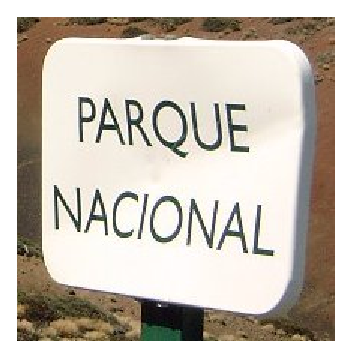
\includegraphics[scale=0.25]{parque-nacional}
    }
  }{label}
\end{pspicture}
\end{LTXexample}
% \iffalse
%</ignore>
% \fi
% 
% \tripoledesc{opttripole}
% \iffalse
%<*ignore>
% \fi
\begin{LTXexample}
\begin{pspicture}(3,3)
  \pnode(0,0){A}
  \pnode(1.5,2){G}
  \pnode(3,1.5){B}
  \opttripole[beam](3,1.5)(1.5,2)(0,0){%
    \rput[b](0,0){text}
  }{label}
\end{pspicture}
\end{LTXexample}
% \iffalse
%</ignore>
% \fi
% \end{ltxsyntax}
% 
% \section{Fiber-Optical Components}\label{sec:fibercomp}
% 
% \subsection{Fiber}
% 
% \begin{ltxsyntax}
% \fiberdipoledesc{optfiber}
% \iffalse
%<*ignore>
% \fi
\begin{LTXexample}
\begin{pspicture}(3,1.5)
  \psset{labeloffset=0.3}
  \optfiber(0,0.5)(3,0.5){SSMF}
\end{pspicture}
\end{LTXexample}
% \iffalse
%</ignore>
% \fi
% \end{ltxsyntax}
% \begin{optionlist}
% \intitem[3]{fiberloops} 
% \iffalse
%<*ignore>
% \fi
\begin{LTXexample}
\begin{pspicture}(3,1.5)
  \psset{labeloffset=0.3}
  \optfiber[fiberloops=2](0,0.5)(3,0.5){SSMF}
\end{pspicture}
\end{LTXexample}
% \iffalse
%</ignore>
% \fi
% 
% \numitem[0.4]{fiberloopradius}
% \iffalse
%<*ignore>
% \fi
\begin{LTXexample}
\begin{pspicture}(3,1.5)
  \psset{labeloffset=0.3}
  \optfiber[fiberloopradius=0.2](0,0.5)(3,0.5){SSMF}
\end{pspicture}
\end{LTXexample}
% \iffalse
%</ignore>
% \fi
% 
% \numitem[0.3]{fiberloopsep}
% \iffalse
%<*ignore>
% \fi
\begin{LTXexample}
\begin{pspicture}(3,1.5)
  \psset{labeloffset=0.3}
  \optfiber[fiberloopsep=0.6](0,0.5)(3,0.5){SSMF}
\end{pspicture}
\end{LTXexample}
% \iffalse
%</ignore>
% \fi
% \end{optionlist}
% 
% \subsection{Amplifier}
% 
% \begin{ltxsyntax}
% \fiberdipoledesc{optamp}
% \iffalse
%<*ignore>
% \fi
\begin{LTXexample}
\begin{pspicture}(3,1.5)
  \optamp(0,1)(3,1){EDFA}
\end{pspicture}
\end{LTXexample}
% \iffalse
%</ignore>
% \fi
% \end{ltxsyntax}
% 
% \begin{optionlist}
% \numitem[0.8]{optampsize} The length of all triangle sides.
% \end{optionlist}
% 
% \subsection{Mach-Zehnder Modulator}
% 
% \begin{ltxsyntax}
% \fiberdipoledesc{optmzm}
% \iffalse
%<*ignore>
% \fi
\begin{LTXexample}
\begin{pspicture}(3,1.5)
  \optmzm(0,1)(3,1){MZM}
\end{pspicture}
\end{LTXexample}
% \iffalse
%</ignore>
% \fi
% \end{ltxsyntax}
% 
% \begin{optionlist}
% \numitem[0.8]{optmzmsize} This is the height of the component, the width
% is \opt{1.6} times the height. Use the \opt{unit} parameter to change this
% relation.
% \end{optionlist}
% 
% \subsection{Filter}
% 
% \begin{ltxsyntax}
% \fiberdipoledesc{optfilter}
% \iffalse
%<*ignore>
% \fi
\begin{LTXexample}
\begin{pspicture}(3,1.5)
  \optfilter(0,1)(3,1){bandpass}
\end{pspicture}
\end{LTXexample}
% \iffalse
%</ignore>
% \fi
% \end{ltxsyntax}
% 
% \begin{optionlist}
% \numitem[0.8]{filtersize}
% \choitem[bandpass]{filtertype}{bandpass, bandstop, lowpass, highpass}
% \iffalse
%<*ignore>
% \fi
\begin{LTXexample}
\begin{pspicture}(3,1.5)
  \optfilter[filtertype=bandstop](0,1)(3,1){bandstop}
\end{pspicture}
\end{LTXexample}
% \iffalse
%</ignore>
% \fi
% \iffalse
%<*ignore>
% \fi
\begin{LTXexample}
\begin{pspicture}(3,1.5)
  \optfilter[filtertype=lowpass](0,1)(3,1){lowpass}
\end{pspicture}
\end{LTXexample}
% \iffalse
%</ignore>
% \fi
% \iffalse
%<*ignore>
% \fi
\begin{LTXexample}
\begin{pspicture}(3,1.5)
  \optfilter[filtertype=highpass](0,1)(3,1){highpass}
\end{pspicture}
\end{LTXexample}
% \iffalse
%</ignore>
% \fi
% \end{optionlist}
% 
% \subsection{Polarization Controller}
% 
% \begin{ltxsyntax}
% \fiberdipoledesc{polcontrol}
% \iffalse
%<*ignore>
% \fi
\begin{LTXexample}
\begin{pspicture}(3,1.5)
  \polcontrol(0,1)(3,1){PC}
\end{pspicture}
\end{LTXexample}
% \iffalse
%</ignore>
% \fi
% \end{ltxsyntax}
% 
% \begin{optionlist}
% \numitem[0.15]{polcontrolsize} The radius of the polarization controller circles.
% \end{optionlist}
% 
% \subsection{Isolator}
% 
% \begin{ltxsyntax}
% \fiberdipoledesc{optisolator}
% \iffalse
%<*ignore>
% \fi
\begin{LTXexample}
\begin{pspicture}(3,1.5)
  \optisolator(0,1)(3,1){isolator}
\end{pspicture}
\end{LTXexample}
% \iffalse
%</ignore>
% \fi
% \end{ltxsyntax}
% 
% \begin{optionlist}
%   \numitem[0.6]{isolatorsize} The height of the isolator. The width is \opt{1.6}
%   times this value. Use the \opt{unit} parameter to change this relation.
% 
% \styleitem{IsolatorArrow} This changes the appearance of the isolator
% arrow. This can be especially useful to adapt the length of the arrow.
% \iffalse
%<*ignore>
% \fi
\begin{LTXexample}
\begin{pspicture}(3,1.5)
  \addtopsstyle{IsolatorArrow}{xunit=1.2, 
                                 arrowinset=0.1}
  \optisolator(0,1)(3,1){isolator}
\end{pspicture}
\end{LTXexample}
% \iffalse
%</ignore>
% \fi
% \end{optionlist}
% 
% \subsection{Optical Switch}
% 
% \begin{ltxsyntax}
% \fiberdipoledesc{optswitch}
% \iffalse
%<*ignore>
% \fi
\begin{LTXexample}
\begin{pspicture}(3,1.5)
  \optswitch(0,1)(3,1){Opened switch}
\end{pspicture}
\end{LTXexample}
% \iffalse
%</ignore>
% \fi
% \end{ltxsyntax}
% 
% \begin{optionlist}
% \numitem[0.8]{switchsize}
% 
% \choitem[opened]{switchstyle}{opened, closed} Indicate the switch as \opt{opened} or \opt{closed}
% \iffalse
%<*ignore>
% \fi
\begin{LTXexample}
\begin{pspicture}(3,1.5)
  \optswitch[switchstyle=closed](0,1)(3,1){Closed switch}
\end{pspicture}
\end{LTXexample}
% \iffalse
%</ignore>
% \fi
% \end{optionlist}
% 
% \subsection{Fiber Delay Line}
% 
% \begin{ltxsyntax}
% \fiberdipoledesc{fiberdelayline}
% \iffalse
%<*ignore>
% \fi
\begin{LTXexample}
\begin{pspicture}](3,1.5)
  \fiberdelayline(0,1)(3,1){Delay line}
\end{pspicture}
\end{LTXexample}
% \iffalse
%</ignore>
% \fi
% \end{ltxsyntax}
% 
% \begin{optionlist}
% \numitem[0.6]{fdlsize}
% \styleitem{FdlArrow} This changes the appearance of the delay line arrow
% and of the arrow type. This can be especially useful to adapt the length of the
% arrow which may not be appropriate depending on the \opt{fdlsize} or to reverse
% the arrow.
% \iffalse
%<*ignore>
% \fi
\begin{LTXexample}
\begin{pspicture}](3,1.5)
  \addtopsstyle{FdlArrow}{xunit=-1}
  \fiberdelayline(0,1)(3,1){Delay line}
\end{pspicture}
\end{LTXexample}
% \iffalse
%</ignore>
% \fi
% \end{optionlist}
% 
% 
% \subsection{Fiber Polarizer}
% 
% \begin{ltxsyntax}
% \fiberdipoledesc{optfiberpolarizer}
% \iffalse
%<*ignore>
% \fi
\begin{LTXexample}
\begin{pspicture}(3,1.5)
  \optfiberpolarizer(0,1)(3,1){polarizer}
\end{pspicture}
\end{LTXexample}
% \iffalse
%</ignore>
% \fi
% \end{ltxsyntax}
% 
% \begin{optionlist}
%   \numitem[0.6]{fiberpolsize}
% \end{optionlist}
% 
% \subsection{Fiber Collimator}
% 
% \begin{ltxsyntax}
% \xLcs{fibercollimator}\cmditem{fibercollimator}(In)(A)(B)(Out){Label}%
% \iffalse
%<*ignore>
% \fi
\begin{LTXexample}
\begin{pspicture}(3,1.5)
  \fibercollimator[beam](0,1)(3,1){FC}
\end{pspicture}
\end{LTXexample}
% \iffalse
%</ignore>
% \fi
% \end{ltxsyntax}
% \begin{optionlist}
% \numitem[0.3]{fibercolsize}
% \end{optionlist}
% The \nxLcs{fibercollimator} can be used with two, three or four points. With two points, the collimator is placed like any other dipole component between \prm{In} and \prm{Out} node. For three nodes, the fiber is drawn as \Lcs{psbezier} curve for which the
% central node \prm{A} is used twice. Positioning parameters can be used to
% shift the object between \prm{In} and \prm{A} nodes.
% 
% \medskip
% 
% \iffalse
%<*ignore>
% \fi
\begin{LTXexample}
\begin{pspicture}(3,2)
   \fibercollimator[beam](0,1)(2,1)(3,2){FC}
\end{pspicture}
\end{LTXexample}
% \iffalse
%</ignore>
% \fi
% 
% \medskip
% 
% For four nodes, the fiber is drawn as \Lcs{psbezier} curve with the specified nodes. Positioning parameters can be used to
% shift the object between \prm{In} and \prm{A} nodes.
% 
% \medskip
% 
% \iffalse
%<*ignore>
% \fi
\begin{LTXexample}
\begin{pspicture}(3,2)
   \fibercollimator[beam](0,1)(2,1)(3,1)(3,2){FC}
\end{pspicture}
\end{LTXexample}
% \iffalse
%</ignore>
% \fi
% 
% \medskip
% 
% \subsection{Coupler}\label{sec:coupler}
% \subsubsection{\texorpdfstring{\mathversion{bold}$2\times 2$}{2x2} Coupler}
% \begin{ltxsyntax}
% \xLfmultipole{optcoupler}\cmditem{optcoupler}(LeftTop)(LeftBottom)(RightTop)(RightBottom){Label}%
% \iffalse
%<*ignore>
% \fi
\begin{LTXexample}
\begin{pspicture}(3,1.5)
  \optcoupler(0,1.5)(0,0.5)(3,1.5)(3,0.5){Coupler}
\end{pspicture}
\end{LTXexample}
% \iffalse
%</ignore>
% \fi
% \end{ltxsyntax}
% \begin{optionlist}
% \numitem[0.2]{couplersize}
% \numitem[0.1]{couplersep} The vertical distance between two fiber ports.
% \iffalse
%<*ignore>
% \fi
\begin{LTXexample}
\begin{pspicture}(3,1.5)
  \optcoupler[couplersep=0]%
               (0,1.5)(0,0.5)(3,1.5)(3,0.5){Coupler}
\end{pspicture}
\end{LTXexample}
% \iffalse
%</ignore>
% \fi
% 
% \choitem[elliptic]{couplertype}{none, elliptic, rectangular, crossswitch}
% \iffalse
%<*ignore>
% \fi
\begin{LTXexample}
\begin{pspicture}(3,4.5)
  \psset{labeloffset=0.5}
  \optcoupler[couplertype=none]%
                (0,4.5)(0,3.5)(3,4.5)(3,3.5){Coupler}
  \optcoupler[couplertype=rectangular]%
               (0,3)(0,2)(3,3)(3,2){Coupler}
  \optcoupler[couplertype=crossswitch]%
               (0,1.5)(0,0.5)(3,1.5)(3,0.5){Coupler}
\end{pspicture}
\end{LTXexample}
% \iffalse
%</ignore>
% \fi
% 
% \choitem[center]{align}{top, bottom, center}
% \iffalse
%<*ignore>
% \fi
\begin{LTXexample}
\begin{pspicture}(3,3)
  \psset{labeloffset=0.4}
  \optcoupler[align=top]%
               (0,3)(0,2)(3,3)(3,2){Top}
  \optcoupler[align=bottom]
               (0,1.5)(0,0.5)(3,1.5)(3,0.5){Bottom}
\end{pspicture}
\end{LTXexample}
% \iffalse
%</ignore>
% \fi
% \end{optionlist}
% 
% \subsubsection{WDM Coupler}
% \begin{ltxsyntax}
% \xLfmultipole{wdmcoupler}\cmditem{wdmcoupler}(LeftTop)(LeftBottom)(Right){Label}%
% \iffalse
%<*ignore>
% \fi
\begin{LTXexample}
\begin{pspicture}(3,1.5)
  \wdmcoupler(0,1.5)(0,0.5)(3,1){WDM}
\end{pspicture}
\end{LTXexample}
% \iffalse
%</ignore>
% \fi
% \end{ltxsyntax}
% 
% \begin{optionlist}
% \numitem[0.2]{couplersize}
% \numitem[0.1]{couplersep} The vertical distance between the two input fiber ports.
% \iffalse
%<*ignore>
% \fi
\begin{LTXexample}
\begin{pspicture}(3,1.5)
  \wdmcoupler[couplersep=0](0,1.5)(0,0.5)(3,1){WDM}
\end{pspicture}
\end{LTXexample}
% \iffalse
%</ignore>
% \fi
% 
% \choitem[elliptic]{couplertype}{none, elliptic, rectangular}
% \iffalse
%<*ignore>
% \fi
\begin{LTXexample}
\begin{pspicture}(3,3)
  \psset{labeloffset=0.5}
  \wdmcoupler[couplertype=none](0,3)(0,2)(3,2.5){WDM}
  \wdmcoupler[couplertype=rectangular]%
               (0,1.5)(0,0.5)(3,1){WDM}
\end{pspicture}
\end{LTXexample}
% \iffalse
%</ignore>
% \fi
% 
% \choitem[center]{align}{top, bottom, center}
% \iffalse
%<*ignore>
% \fi
\begin{LTXexample}
\begin{pspicture}(3,3)
  \psset{labeloffset=0.4}
  \wdmcoupler[align=top,
                couplertype=none](0,3)(0,2)(3,3){Top}
  \wdmcoupler[align=bottom]
               (0,1.5)(0,0.5)(3,0.5){Bottom}
\end{pspicture}
\end{LTXexample}
% \iffalse
%</ignore>
% \fi
% \end{optionlist}
% 
% \subsubsection{WDM Splitter}
% \begin{ltxsyntax}
% \xLfmultipole{wdmcoupler}\cmditem{wdmsplitter}(Left)(RightTop)(RightBottom){Label}%
% \iffalse
%<*ignore>
% \fi
\begin{LTXexample}
\begin{pspicture}(3,1.5)
  \wdmsplitter(0,1)(3,1.5)(3,0.5){WDM}
\end{pspicture}
\end{LTXexample}
% \iffalse
%</ignore>
% \fi
% \end{ltxsyntax}
% \begin{optionlist}
% \numitem[0.2]{couplersize}
% \numitem[0.1]{couplersep} The vertical distance between the two output fiber ports.
% \iffalse
%<*ignore>
% \fi
\begin{LTXexample}
\begin{pspicture}(3,1.5)
  \wdmsplitter[couplersep=0](0,1)(3,1.5)(3,0.5){WDM}
\end{pspicture}
\end{LTXexample}
% \iffalse
%</ignore>
% \fi
% 
% \choitem[elliptic]{couplertype}{none, elliptic, rectangular}
% \iffalse
%<*ignore>
% \fi
\begin{LTXexample}
\begin{pspicture}(3,3)
  \psset{labeloffset=0.5}
  \wdmsplitter[couplertype=none](0,2.5)(3,3)(3,2){WDM}
  \wdmsplitter[couplertype=rectangular]%
                 (0,1)(3,1.5)(3,0.5){Coupler}
\end{pspicture}
\end{LTXexample}
% \iffalse
%</ignore>
% \fi
% 
% \choitem[center]{align}{top, bottom, center}
% \iffalse
%<*ignore>
% \fi
\begin{LTXexample}
\begin{pspicture}(3,3)
  \psset{labeloffset=0.4}
  \wdmsplitter[align=top,
                 couplertype=none](0,3)(3,3)(3,2){Top}
  \wdmsplitter[align=bottom](0,0.5)(3,1.5)(3,0.5){Bottom}
\end{pspicture}
\end{LTXexample}
% \iffalse
%</ignore>
% \fi
% \end{optionlist}
% 
% 
% \section{Connecting Objects}\label{sec:connecting}
% 
% The package provides several methods for automatic beam and fiber
% drawing which are two fundamentally different way of connecting.
% 
% \subsection{Accessing Objects}
% 
% The macro arguments, specified as Obj$_1$, Obj$_2$, \ldots Obj$_N$ in
% the following macro definitions, can be either objects or PSTricks
% nodes. To distinguish between named nodes (see \prettyref{sec:namedobj})
% and object names, the node content must be enclosed in parenthesis
% within the brackets. Components can either be assigned a name
% explicitely using the \Lkeyword{compname} parameter, or they get a
% unique number in ascending order by their definition in the code. If the
% argument is left empty, the last object is used.
% 
% \iffalse
%<*ignore>
% \fi
\begin{LTXexample}
\begin{pspicture}(3,1.5)
  \pnode(0,1){A}\pnode(1.5,1){B}
  \optbox[endbox, labeloffset=0](A)(B){1}
  % connect an object by its automatic number
  \drawbeam{(A)}{1}
\end{pspicture}
\end{LTXexample}
% \iffalse
%</ignore>
% \fi
% 
% \medskip
% 
% \iffalse
%<*ignore>
% \fi
\begin{LTXexample}
\begin{pspicture}(3,2)
  \psset{endbox, labeloffset=0}
  \optbox[compname=obj](0,1)(1.5,1){obj}
  % connect an object by its compname
  \drawbeam{(0,1)}{obj}
\end{pspicture}
\end{LTXexample}
% \iffalse
%</ignore>
% \fi
% 
% \medskip
% 
% The objects which have an explicit \Lkeyword{compname} also increase the internal
% counter, so that removing the \nxLkeyword{compname} from an intermediate
% object does not affect the numbering of the following ones.
% 
% \medskip
% 
% \iffalse
%<*ignore>
% \fi
\begin{LTXexample}
\begin{pspicture}(3,2)
  \psset{endbox, labeloffset=0}
  \optbox[compname=obj](0,0.5)(1.5,0.5){obj}
  \optbox(0,1.5)(1.5,1.5){2}
  % named objects are also numbered
  \drawbeam{(0,1)}{2}
\end{pspicture}
\end{LTXexample}
% \iffalse
%</ignore>
% \fi
% 
% \medskip
% 
% \iffalse
%<*ignore>
% \fi
\begin{LTXexample}
\begin{pspicture}(3,2)
  \psset{endbox, labeloffset=0}
  \optbox(0,0.5)(1.5,0.5){1}
  \optbox(0,1.5)(1.5,1.5){2}
  % an empty argument refers to the last object
  \drawbeam{(0,1)}{}
\end{pspicture}
\end{LTXexample}
% \iffalse
%</ignore>
% \fi
% 
% \subsection{Drawing beams}\label{sec:drawbeam}
% 
% \begin{ltxsyntax}
%   \xLcs{drawbeam}\cmditem{drawbeam}[Options]{Obj$_1$}{Obj$_2$}{\ldots}{Obj$_N$}
%   \xLcs{drawwidebeam}\cmditem{drawwidebeam}[Options]{Obj$_1$}{Obj$_2$}{\ldots}{Obj$_N$}
% \end{ltxsyntax}
% The package provides two macros for connecting objects with beams. Most
% parameters are valid for both, those which are specified for wide beams
% are demonstrated separately in the next section.
% 
% \begin{optionlist}
%   \optitem[0]{startpos}{[\prm{X}] \prm{Y}} This is the start position
%   (\prm{X}, \prm{Y}) of the beam at the first interface. Can be any code
%   which evaluates in Postscript to one or two numbers. If is only one
%   number then the $x$-coordinate is set to \texttt{0}.
% 
% \medskip
% 
% \iffalse
%<*ignore>
% \fi
\begin{LTXexample}
\begin{pspicture}(4,2.8)
  \pnode(1.5,0.5){A}\pnode(3.5,0.5){B}
  \pnode(3.5,2.5){C} 
  \optbox[endbox](B)(A){}
  \psset{mirrortype=extended, mirrordepth=0.15}
  \mirror[mirrorradius=2](A)(B)(C){} 
  \mirror(B)(C)(B){} 
  \drawbeam[linecolor=red, 
              startpos=-0.2]{1}{2}{3}
  \drawbeam[linecolor=blue]{1}{2}{3}
  \drawbeam[linecolor=green,
              startpos=0.2]{1}{2}{3}
\end{pspicture}
\end{LTXexample}
% \iffalse
%</ignore>
% \fi
% 
% \optitem[1]{startvec}{\prm{X} [\prm{Y}]} 
% This is the start vector (\prm{X}, \prm{Y}) of the beam. \prm{X} and
% \prm{Y} can be anything which evaluates to a number in Postscript. If
% only one value is given, \prm{X} is set to \opt{0}. The
% \nxLkeyword{startvec} is relative to the connection between the first
% two components, use \Lkeyword{startvecabs} to change this.
% 
% \medskip
% \iffalse
%<*ignore>
% \fi
\begin{LTXexample}
\begin{pspicture}(4,3)
  \pnode(1.5,0.5){A}\pnode(3.5,0.5){B}
  \pnode(3.5,2.5){C} 
  \psset{mirrortype=extended, mirrordepth=0.15}
  \optbox[endbox](B)(A){}
  \mirror(A)(B)(C){} 
  \mirror(B)(C)(B){} 
  \drawbeam[linecolor=red, 
              startvec=0.05]{1}{2}{3}
  \drawbeam[linecolor=blue]{1}{2}{3}
  \drawbeam[linecolor=green, 
              startvec=-0.05]{1}{2}{3}
\end{pspicture}
\end{LTXexample}
% \iffalse
%</ignore>
% \fi
% 
% \medskip
% 
% \boolitem[false]{startvecabs}
% 
% \boolitem[false]{connectplanes}
% 
% \numitem[1.5]{n}
% 
% \boolitem[false]{beaminside}
% 
% \boolitem[false]{beaminsidelast}
% 
% \boolitem[false]{beaminsidefirst}
% \end{optionlist}
% 
% \subsubsection{Internal component structure}
% 
% In order to understand properly how the automatic beam drawing actually works,
% it is necessary to describe in more detail the internal component structure.
% 
% Every component type consists internally of interfaces which are defined by a
% node on the optical axis, a plane vector or a curvature radius, and by its
% optical characteristic (reflective or transmittive). The interface nodes can be
% visualized for each component type with the \Lkeyword{showifcnodes}
% parameter. 
% 
% \medskip
% 
% \iffalse
%<*ignore>
% \fi
\begin{LTXexample}
\begin{pspicture}(4,3)
  \psset{showifcnodes}
  \optbox(0,2.5)(4,2.5){}
  \doveprism(0,1.5)(4,1.5){}
  \lens(0,0.5)(4,0.5){}
  \mirror(0,0.5)(3.5,0.5)(3.5,3){}
\end{pspicture}
\end{LTXexample}
% \iffalse
%</ignore>
% \fi
% 
% \bigskip
% 
% \nxLcs{draw*beam} calculates the distance between the interface nodes of two
% objects and connects the two nearest
% 
% \medskip
% 
% \iffalse
%<*ignore>
% \fi
\begin{LTXexample}
\begin{pspicture}(-2,-2)(2,2)
  \psset{optboxwidth=0.6, optboxheight=0.5, labeloffset=0}
  \multido{\i=0+60,\ii=1+1}{6}{%
    \pnode(1.75;\i){A}
    \optbox([Xnodesep=-1]A)([Xnodesep=1]A){\ii}
  }
  \optbox[compname=ref](-1,0)(1,0){ref}
  \addtopsstyle{Beam}{arrows=->}
  \multido{\i=1+1}{6}{\drawbeam{ref}{\i}}
\end{pspicture}
\end{LTXexample}
% \iffalse
%</ignore>
% \fi
% 
% \subsection{Drawing wide beams}\label{sec:drawwidebeam}
% 
% \begin{optionlist}
% \numitem[0.1]{beamwidth}
% 
% \numitem[0]{beamdiv}
% \end{optionlist}
% 
% \subsection{Drawing fibers}\label{sec:drawfiber}
% 
% Fiber-optical objects are automatically connected to the reference
% nodes. The style of all fiber connections can be configured
% independently (see Sec.~\ref{sec:fiberstyles}).
%
% This works quiet well if the components are aligned serially, but ceases to
% give good result for more complicated situations. In that case single or all
% fiber can be omitted and drawn separately.
%
% \subsubsection{Automatic fiber connections}
%
% All fiber-optical components described in \prettyref{sec:fibercomp} are
% connected automatically to their reference nodes with \Lcs{pccurve}. The
% styles of the fiber connections can be configured independently by the
% styles shown in \prettyref{fig:style-inheritance}.
%
% \begin{figure}\centering
% \begin{pspicture}(10,4.4)
% \rput[lt](0,4.4){\pstree[levelsep=1.5cm, treesep=0.4, nodesep=5pt, arrows=<-, arrowinset=0, arrowscale=1.5]{\poeTR{Fiber}}{%
%   \pstree{\poeTR{FiberIn}}{\poeTR{FiberIn1} \poeTR{FiberIn2}}
%   \pstree{\poeTR{FiberOut}}{\poeTR{FiberOut1} \poeTR{FiberOut2}}}
% \rput[l](-1,0|T-0){parent style}
% \rput[l](-1,0|T-0-0){\parbox{\widthof{outgoing fibers}}{\RaggedRight incoming and outgoing fibers}}
% \rput[t](! \psGetNodeCenter{T-0-0-0} \psGetNodeCenter{T-0-0-1}
%         T-0-0-0.x T-0-0-1.x add 2 div T-0-0-0.y 0.4 sub){%
%           \parbox{3.8cm}{\RaggedRight Upper(1) or lower(2) incoming fiber.}}
% \rput[t](! \psGetNodeCenter{T-0-1-0} \psGetNodeCenter{T-0-1-1}
%         T-0-1-0.x T-0-1-1.x add 2 div T-0-1-0.y 0.4 sub){%
%           \parbox{3.8cm}{\RaggedRight Upper(1) or lower(2) outgoing fiber.}}}
% \end{pspicture}
% \caption{Inheritance diagram for the psstyles used for the automatic fiber
%   connections. These style should be changed with \protect\Lcs{addtopsstyle} as not to
%   destroy the inheritance.}\label{fig:style-inheritance}
% \xLstyle{Fiber}\xLstyle{FiberIn}\xLstyle{FiberIn1}\xLstyle{FiberIn2}
% \xLstyle{FiberOut}\xLstyle{FiberOut1}\xLstyle{FiberOut2}
% \end{figure}
%
% \begin{optionlist}
% \item[\smash{\begin{tabular}[t]{@{}r}\opt{new}\prm{style}\\\opt{addto}\prm{style}\end{tabular}}]
%   \xLkeyword{newFiber}\xLkeyword{addtoFiber}
%   \xLkeyword{newFiberIn}\xLkeyword{addtoFiberIn}
%   \xLkeyword{newFiberIn1}\xLkeyword{addtoFiberIn1}
%   \xLkeyword{newFiberIn2}\xLkeyword{addtoFiberIn2}
%   \xLkeyword{newFiberOut}\xLkeyword{addtoFiberOut}
%   \xLkeyword{newFiberOut1}\xLkeyword{addtoFiberOut1}
%   \xLkeyword{newFiberOut2}\xLkeyword{addtoFiberOut2} For every style two
%   appropriate keys \opt{new}\prm{style} and \opt{addto}\prm{style} are
%   provided which can be used to change the styles for only one object. This
%   can be used to define own components with respectively changed fiber
%   connections or to avoid grouping.
%
%   \boolitem{fiber} Some components can be used either for free-ray or
%   fiber-optical setups (\Lcs{optbox}, \Lcs{optdetector}). The \opt{fiber}
%   parameter enables automatic fiber connections for them.
%
% \iffalse
%<*ignore>
% \fi
\begin{LTXexample}
\begin{pspicture}(3,2)
  \addtopsstyle{FiberIn}{ArrowInside=->, 
                           arrowscale=1.5,
                           arrowinset=0}
  \optbox[fiber](0,1)(3,1){}
\end{pspicture}
\end{LTXexample}
% \iffalse
%</ignore>
% \fi
%
% \paragraph{Fiber angles}
%
% The angles of the fiber connections are calculated automatically from the orientation of the component.
%
% \iffalse
%<*ignore>
% \fi
\begin{LTXexample}
\begin{pspicture}(3,2)
  \optbox[angle=20, fiber](0,1)(3,1){}
\end{pspicture}
\end{LTXexample}
% \iffalse
%</ignore>
% \fi
%
% \iffalse
%<*ignore>
% \fi
\begin{LTXexample}
\begin{pspicture}(3,2)
  \optbox[compshift=0.5, fiber](0,1)(3,1){}
\end{pspicture}
\end{LTXexample}
% \iffalse
%</ignore>
% \fi
% \end{optionlist}
% 
% \subsubsection{Manual fiber connections}
%
% \begin{ltxsyntax}
%   \xLcs{drawfiber}\cmditem{drawfiber}[Options]{Obj$_1$}{Obj$_2$}
% \end{ltxsyntax}
% 
% \begin{optionlist}
% \boolitem{usefiberstyle}
% For some components it might me nice to highlight some
% internals. If \Lkeyword{usefiberstyle} is enabled, for examples the
% passing parts of the optical filter are drawn with the \styleshape{Fiber}
% style. In the documentation this parameter is enabled to show the parts
% which would be highlighted.
% \end{optionlist}
% 
% \begin{optionlist}
%   \boolitem{relangle}
%   \choitem{startnode}{auto, 1, 2, 3, 4, N}
% \iffalse
%<*ignore>
% \fi
\begin{LTXexample}
\begin{pspicture}(4,3)
  \pnode(0,0.5){A}\pnode(2,0.5){B}
  \pnode([offset=1]B){C}\pnode(A|C){D}
  \optamp[nofiber](A)(B){EDFA}
  \optbox(C)(D){PM}
  \drawfiber[linecolor=black]{1}{2}
\end{pspicture}
\end{LTXexample}
% \iffalse
%</ignore>
% \fi
% 
% \choitem{stopnode}{auto, 1, 2, 3, 4, N}
% \end{optionlist}
% 
% \iffalse
%<*ignore>
% \fi
\begin{LTXexample}
\begin{pspicture}(2.1,3)
\pnode(0,0){A}\pnode(2,0){B}
\pnode(0.3,3){C}\pnode(1.7,3){D}
\optcoupler[fiberout=none,
            addtoFiberIn1={angleA=0, ArrowInside=->},
            addtoFiberIn2={angleA=180, arrows=<-},
            abspos=0.5, compname=Cpl](A)(B)(C)(D){}
\optfiber[nofiber, compname=Hnlf, abspos=1](C)(C|A){}
\optamp[nofiber, abspos=2, compname=Amp](D|B)(D){}
\drawfiber{Cpl}{Hnlf}
\drawfiber[startnode=1, stopnode=N, ncurv=1.2]{Hnlf}{Amp}
\drawfiber{Cpl}{Amp}
\end{pspicture}
\end{LTXexample}
% \iffalse
%</ignore>
% \fi
% 
% \subsubsection{Fiber Styles}\label{sec:fiberstyles}
% 
% The appearence of the fiber parts before and after each object can be changed
% with several styles (see \ref{sec:styles}). On the left side of the components
% are the input connections and on the right side the output connections.
% 
% \begin{optionlist}
% 
% \styleitem{Fiber}
% This is the basic style from which every other fiber style inherits.
% 
% \iffalse
%<*ignore>
% \fi
\begin{LTXexample}
\begin{pspicture}(3,1.5)
  \addtopsstyle{Fiber}{linecolor=blue}
  \optamp(0,1)(3,1){}
\end{pspicture}
\end{LTXexample}
% \iffalse
%</ignore>
% \fi
% 
% \styleitem[style=Fiber]{FiberIn}
% Controls the fibres on the left side of the component. Inherits from \nxLstyle{Fiber}.
% 
% \iffalse
%<*ignore>
% \fi
\begin{LTXexample}
\begin{pspicture}(3,1.5)
  \addtopsstyle{FiberIn}{linecolor=blue}
  \optamp(0,1)(3,1){}
\end{pspicture}
\end{LTXexample}
% \iffalse
%</ignore>
% \fi
% 
% \styleitem[style=FiberIn]{FiberIn1}
% \styleitem[style=FiberIn]{FiberIn2}
% If the component has two input fibers, \nxLstyle{FiberIn1} sets the style of the
% upper one and \nxLstyle{FiberIn2} the style of the lower fiber. Otherwise these
% styles are ignored.
% 
% \iffalse
%<*ignore>
% \fi
\begin{LTXexample}
\begin{pspicture}(3,1.5)
  \addtopsstyle{FiberIn1}{linecolor=blue}
  \addtopsstyle{FiberIn2}{linecolor=green}
  \optcoupler(0,1.5)(0,0)(3,1.5)(3,0){}
\end{pspicture}
\end{LTXexample}
% \iffalse
%</ignore>
% \fi
% 
% \styleitem[style=Fiber]{FiberOut}
% \styleitem[style=FiberOut]{FiberOut1}
% \styleitem[style=FiberOut]{FiberOut2}
% \end{optionlist}
% 
% \medskip
% 
% In addition to the psstyles there exist
% corresponding \Lkeyword{newFiber\ldots} and \Lkeyword{addtoFiber\ldots}
% parameter keys for each of them.
% 
% \medskip
% 
% \begin{lstlisting}[gobble=2]
% \psset{addtoFiberIn={arrows=->, arrowscale=1.3}}
% \end{lstlisting}
% 
% \medskip
% 
% \noindent is equivalent to 
% 
% \medskip
% 
% \begin{lstlisting}[gobble=2]
% \addtopsstyle{FiberIn}{arrows=->, arrowscale=1.3}
% \end{lstlisting}
% 
% \medskip
% 
% \noindent Accordingly \Lkeyword{newFiberIn} corresponds to \Lcs{newpsstyle\{FiberIn\}\{\ldots\}}.
% 
% At first glance these keys make no sense. The reason why I
% introduced them was to be able to define special couplers with
% \Lcs{newpsobject}. This is only possible if all modifications can be
% expressed as parameter keys. Consider for example a WDM splitter which
% only couples out a certain spectral range of the input and you want to
% mark the output with an arrow:
% 
% \medskip
% 
% \iffalse
%<*ignore>
% \fi
\begin{LTXexample}[width=3.5cm]
\begin{pspicture}[showgrid=true](3,2)
   \newpsobject{mywdmsplitter}{wdmsplitter}{addtoFiberOut1={arrows=->, arrowscale=1.3, linecolor=blue}, labelangle=180, align=bottom}
   \mywdmsplitter(0,0.5)(3,1.5)(3,0.5){blue band}
\end{pspicture}
\end{LTXexample}
% \iffalse
%</ignore>
% \fi
% 
% \medskip
% 
% Or if you need a coupler with a particular input angle you can do it be extending the appropriate fiber style:
% 
% \medskip
% 
% \iffalse
%<*ignore>
% \fi
\begin{LTXexample}[width=3.5cm]
\begin{pspicture}[showgrid=true](3,2)
   \newpsobject{mycoupler}{optcoupler}{addtoFiberIn2={angleA=90}, align=top}
   \mycoupler(0.5,1.5)(0.5,0.5)(2.5,1.5)(2.5,0.5){}
\end{pspicture}
\end{LTXexample}
% \iffalse
%</ignore>
% \fi
% 
% \medskip
% 
% \subsection{Custom beams}\label{sec:custombeam}
% \begin{ltxsyntax}
%   \xLcs{custombeam}\cmditem{custombeam}[Options]{\nxLcs{draw*beam}}
% \end{ltxsyntax}
% 
% \begin{optionlist}
% \boolitem[false]{startinside}
% 
% \boolitem[false]{stopinside}
% \end{optionlist}
% 
% 
% \section{Defining New Objects}
% 
% \subsection{Customized Versions of Existing Macros}
% 
% The easiest way to define your own components is to use the
% \Lcs{newpsobject} macro. With this you can define a new component using
% predefined objects with a set of options. These options serve only as
% default values and can be overridden when calling the macro. The
% following examples defines a new object \nxLcs{sbn} for the special crystal
% used in Sec.~\ref{sec:crystal}.
% 
% \medskip
% 
% \iffalse
%<*ignore>
% \fi
\begin{LTXexample}[width=3.5cm]
\newpsobject{sbn}{crystal}{voltage, lamp, labelangle=45, labeloffset=1.2, fillstyle=solid, fillcolor=yellow!90!black}
\begin{pspicture}[showgrid=true](3,2) 
   \sbn(0,1)(3,1){SBN:Ce}
   \psline[style=Beam](0,1)(3,1)
\end{pspicture}
\end{LTXexample}
% \iffalse
%</ignore>
% \fi
% 
% \medskip
% 
% \iffalse
%<*ignore>
% \fi
\begin{LTXexample}[width=3.5cm]
\newpsobject{pumpcoupler}{wdmcoupler}{align=top, labelangle=180, labeloffset=0.5,addtoFiberIn2={ArrowInside=->, arrowscale=2}}
\begin{pspicture}[showgrid=true](3,2) 
   \pumpcoupler(0,1)(0,0)(3,1){Pumpcoupler}
\end{pspicture}
\end{LTXexample}
% \iffalse
%</ignore>
% \fi
% 
% \medskip
% 
% Or if you need more than one type of lenses several times in your setup
% it is very cumbersome to specify all parameters every time.
% 
% \medskip
% 
% \iffalse
%<*ignore>
% \fi
\begin{LTXexample}[width=5.5cm]
\newpsobject{MOLensIn}{lens}{lens=0.5 0.5 0.5}
\newpsobject{MOLensOut}{lens}{lens=1.5 1.5 1.5}
\begin{pspicture}[showgrid=true](5,2) 
   \pnode(0,1){A}\pnode(5,1){B}
   \psset{n=1}
   \MOLensIn[abspos=0.5](A)(B){}
   \MOLensOut[abspos=1](A)(B){}
   \MOLensOut[abspos=4](A)(B){}
   \MOLensIn[abspos=4.5](A)(B){}
   \custombeam{%
     \drawwidebeam[beamwidth=0.1]{(A)}{1}
     \drawwidebeam[beamdiv=1]{1}{2}
   }
\end{pspicture}
\end{LTXexample}
% \iffalse
%</ignore>
% \fi
% \medskip
% 
% \subsection{Defining New Objects}\label{sec:newobj}
% 
% Since version 1.2 \nxLPack{pst-optexp} provides some high-level macros to
% allow very convenient definition of completely new components. The macro
% \Lcs{newOptexpDipole} generates all organizing code for a new free-ray
% component. All you have to do is to define a new `drawing' macro
% \nxLcs{mycomponent@iii} which contains all drawing code. Analogously
% \Lcs{newOptexpDipoleNolabel} defines a new free-ray object without label
% (like \Lcs{polarization}) and \Lcs{newOptexpTripole} defines a new
% reflective component. 
% 
% New fiber-optical components can be defined using
% \Lcs{newOptexpFiberDipole}. This macro differs from its free-ray
% analogous only in that it presets \Lkeyword{fiber} and hence directly
% connects the component with its reference nodes. The first node in the
% parameter list gets connected with a node \nodename{tempNode@A@}, the
% second node with a node \nodename{tempNode@B@}. These two internal
% nodes are preset to \paramvalue{(0,0)} and can be overwritten within the
% drawing macro.
% 
% The syntax of the macros is
% \begin{lstlisting}[gobble=2]
% \newOptexpDipole[fixed options]{name}{default options}
% \newOptexpDipoleNolabel[fixed options]{name}{default options}
% \newOptexpTripole[fixed options]{name}{default options}
% \newOptexpFiberDipole[fixed options]{name}{default options}
% \end{lstlisting}
% The \texttt{default options} are simply a list of PSTricks parameters
% which are taken as defaults for the new component. The optional argument
% allows setting of parameters which cannot be overridden later.
% 
% This is illustrate a bit more in the next code snippet, which also shows
% how the coordinate system is handled within the \nxLcs{mycomponent@iii}
% macro.
% 
% \medskip
% 
% \iffalse
%<*ignore>
% \fi
\begin{LTXexample}[width=4.5cm]
\newOptexpTripole{mygrid}{subgriddiv=5, griddots=0, subgridwidth=\pslinewidth, gridwidth=2\pslinewidth}
\makeatletter
\def\mygrid@iii{% put here all PSTricks drawing code
  \psgrid(-1,0)(1,1)
}%
\makeatother
\begin{pspicture}[showgrid=true](4,4) 
   \pnode(0,1){A}\pnode(2,2){G}\pnode(3,0){B}
   \mygrid[gridcolor=red,labeloffset=1.5](A)(G)(B){myGrid}
   \psline[style=Beam](A)(G)(B)
\end{pspicture}
\end{LTXexample}
% \iffalse
%</ignore>
% \fi
% \medskip
% 
% The default position of the label reference point is (0,0). If you want
% to change this, you have to define a new pnode named
% \nodename{tempNode@Label} in the \nxLcs{mycomponent@iii} macro.
% 
% If you create a new component, please send it to me then I can
% incorporate this in a new released version.
% 
% \newpage
% 
% \section{Examples}
% \iffalse
%<*ignore>
% \fi
\begin{LTXexample}[pos=t,vsep=8mm]
\begin{pspicture}(10,2)
\psset{optboxwidth=1}\addtopsstyle{Beam}{linewidth=2\pslinewidth}
\pnode(1,1){Start}\pnode(9,1){CCD}\optbox[endbox, labeloffset=0](CCD)(Start){Laser}
\optbox[endbox,labeloffset=0,beam](Start)(CCD){CCD}
\polarization[poltype=perp,abspos=0.5](Start)(CCD)
\optretplate[abspos=1](Start)(CCD){$\nicefrac{\lambda}{2}$}
\lens[lens=0.4 0.4 0.5,abspos=2](Start)(CCD){$L_1$}\lens[abspos=4](Start)(CCD){$L_2$}
\optplate[abspos=6,platelinewidth=3\pslinewidth](Start)(CCD){SLM}
\optplate[abspos=6.5,labelangle=180](Start)(CCD){PF}
\polarization[abspos=6.7](Start)(CCD)\lens[abspos=7](Start)(CCD){$L_3$}
\end{pspicture}
\end{LTXexample}
% \iffalse
%</ignore>
% \fi
% 
% \vspace{\fill}
% 
% \iffalse
%<*ignore>
% \fi
\begin{LTXexample}[pos=t,vsep=8mm]
\begin{pspicture}(-4,-1)(3,3)
\addtopsstyle{Beam}{linewidth=2\pslinewidth, linecolor=red!90!black}
\psset{labeloffset=0.5}
\pnode(-2,0){LaserOut}\pnode(0,0){Grat}
\pnode(4;45){Out}\pnode(2.5;67.5){Mvar}
\optbox[optboxwidth=2,labeloffset=0, endbox](Grat)(LaserOut){diode laser}
%\mirror[variable,conn=o-](Grid)(Mvar)(Grid){M$_\mathrm{var}$}
\optgrid[beam](LaserOut)(Grat)(Out){grating}
\optretplate[position=0.3,labeloffset=0.8]%
  (LaserOut)(Grat){$\nicefrac{\lambda}{4}$}
\rput[l](-3,2){Littman setup}
\end{pspicture}
\end{LTXexample}
% \iffalse
%</ignore>
% \fi
% 
% \iffalse
%<*ignore>
% \fi
\begin{LTXexample}[pos=t, vsep=8mm]
\begin{pspicture}(8.5,1.6)
    \addtopsstyle{Beam}{linecolor=green!90!black}
    \pnode(1.6,1){Laser}\pnode(7.6,1){Diode}
    \optbox[endbox,labeloffset=0](Diode)(Laser){Laser}%
%    \optbox[abspos=4, optboxwidth=1, optboxheight=0.6, labeloffset=1, compname=PC, conn=o-, angle=-10, rotateref=l, refractiveindex=2.3](Laser)(Diode){Photonic Crystal}
%    \optdetector[dettype=diode, conn=o-](\oenodeout{PC})(Diode|\oenodeout{PC}){PD}
    \optbox[abspos=4, optboxwidth=1, optboxheight=0.6, labeloffset=1, compname=PC, angle=-10, rotateref=l, refractiveindex=2.3](Laser)(Diode){Photonic Crystal}
    \optdetector[dettype=diode](\oenodeout{PC})(Diode|\oenodeout{PC}){PD}
    \nodexn{(\oenodein{PC}) + (2;170)}{Angle1}
    \psline[linestyle=dashed](\oenodein{PC})(Angle1)
    \psarc{<->}(\oenodein{PC}){1.3}{330}{30}
    \psarc[arcsep=1pt]{<->}(\oenodein{PC}){2}{170}{180}
    \uput{2.1}[175](\oenodein{PC}){\small $\varphi$}
\end{pspicture}
\end{LTXexample}
% \iffalse
%</ignore>
% \fi
% 
% \iffalse
%<*ignore>
% \fi
\begin{LTXexample}[pos=t, vsep=8mm]
\begin{pspicture}(6.4,3.2)
  \addtopsstyle{Fiber}{linecolor=red}
  \pnode(2.3,2.3){Lin}\pnode([Xnodesep=0.5]Lin){Lout}
  \pnode([Xnodesep=1.5]Lout){EAMout}
  \pnode([Xnodesep=1.5]EAMout){Det}
  \optbox[fiber, label=-0.2, endbox, compname=L, extnode=b](Lout)(Lin){%
    \psGauss[yunit=0.03,sigma=0.03]{-0.5}{0.5}}
  \optbox[fiber, label=0, optboxwidth=1, compname=EAM, extnode=b](Lout)(EAMout){EAM}
  \optfiber[labeloffset=0.3](EAMout)(Det){fibre}
  \optdetector(EAMout)(Det){OSA}
  \pnode([Xnodesep=-1,offset=-1]\oenodeext{L}){Osc}
  \pnode(\oenodeext{L}|Osc){PSin}\pnode(\oenodeext{EAM}|Osc){PSout}
  \oscillator[output=right](Osc){10\,GHz}{}
  \phaseshifter[arrowscale=1.5, inputarrow, labeloffset=-0.7](PSin)(PSout){$\tau$}
  \psset{arrows=->, arrowinset=0, arrowscale=1.5}
  \wire(PSin)(\oenodeext{L})
  \wire(PSout)(\oenodeext{EAM})
\end{pspicture}
\end{LTXexample}
% \iffalse
%</ignore>
% \fi
% 
% \iffalse
%<*ignore>
% \fi
\begin{LTXexample}[pos=t, vsep=5mm]
\begin{pspicture}(0.9,0.9)(10.4,5.9)
  \psset{arrowscale=1.5, arrowinset=0}
  \pnode(2,5){PC1in}\pnode(4,5){PC1out}\pnode(6,5){PC2in}
  \pnode(8,5){PC2out}\pnode(2,2){CplSig}\pnode(5,2){CplIn}
  \pnode(2,1){CplOut}\pnode(10,4.5){Pump}\pnode(8,2){PumpSig}
  \optisolator[compshift=0.8, addtoFiberIn={angleA=180}, 
                 addtoFiberOut={angleB=180}, label=0.5 . l]%
                 (CplSig)(PC1in){isolator}
  \polcontrol[addtoFiberIn={arrows=|-}](PC1in)(PC1out){}
  \optfiberpolarizer[labeloffset=0.6](PC1out)(PC2in){polarizer}
  \polcontrol[addtoFiberOut={arrows=-|}](PC2in)(PC2out){}
  \wdmsplitter[labeloffset=0.3, align=bottom, addtoFiberIn={arrows=|-}, 
                 addtoFiberOut1={arrows=->}, addtoFiberOut2={arrows=-|}]%
                 (CplIn)(CplOut)(CplSig){95/5}
  \wdmcoupler[addtoFiberIn1={ArrowInside=->}, addtoFiberIn2={angleA=0}, 
                addtoFiberOut={angleB=0,arrows=-|}, ncurv=0.9, 
                align=bottom, compshift=0.8](Pump)(PC2out)(PumpSig){Pump}
  \optbox[endbox, label=0 . . relative]([offset=-0.1]Pump)(Pump){980~nm}
  \optfiber[fiberloops=2, labeloffset=0.4](CplIn)(PumpSig){Er$^+$-doped}
\end{pspicture}
\end{LTXexample}
% \iffalse
%</ignore>
% \fi
% 
% \iffalse
%<*ignore>
% \fi
\begin{LTXexample}[pos=t, vsep=8mm]
\makeatletter
\def\LCLV@nodes{%
  \newOptexpComp{ {-0.12 0} {0 1} trans {NewPlaneInt}
                  {0.15 0} {0 1} trans {NewPlaneInt} \poe@key@n}%
}%
\def\LCLV@comp{%
  \psframe[fillstyle=solid,fillcolor=black,dimen=outer](-0.12,-0.5)(0,0.5)
  \psframe[fillstyle=solid,fillcolor=gray!50,dimen=outer](0,-0.5)(0.15,0.5)
}%
\makeatother
\begin{pspicture}(9,5)
\newOptexpDipole{LCLV}{}\psset{lens=1.2 0 1}
\pnode(2.4,1){BS1}\pnode([offset=3]BS1){M1}\pnode([Xnodesep=5.5]M1){PP}\pnode(PP|BS1){BS2}
\LCLV[position=0.2, compname=LCLV](BS1)(BS2){LCLV}\beamsplitter[compname=BS](BS2)(BS1)(M1){BS}
\optretplate(BS1)(M1){P}\mirror(BS1)(M1)(PP){M}\lens[position=0.2](M1)(PP){L}
\pinhole(M1)(PP){}\lens[position=0.2](PP)(M1){L}\pentaprism(M1)(PP)(BS2){PP}
\beamsplitter(PP)(BS2)(BS1){BS}\lens(BS2)(BS1){L}
\doveprism[compname=Dove,position=0.27](BS2)(BS1){D}
\addtopsstyle{Beam}{arrowscale=1.3, ArrowInside=-<}
\optbox[labeloffset=0, endbox](BS1)([Xnodesep=-1]BS1){Nd:YAG}
\drawbeam{LCLV}{BS}
\end{pspicture}
\end{LTXexample}
% \iffalse
%</ignore>
% \fi
% 
% \begin{pspicture}(0,-0.4)(9,6)
%   \addtopsstyle{Beam}{linewidth=2\pslinewidth}
%   \pnode(1.5,5){Laser}\pnode(4,5){PBS}\pnode(6.5,5){PBS2}
%   \pnode(6.5,5.7){piezo}\pnode(4,2){BSFwd}\pnode(6.5,2){BSBwd}
%   \pnode(2,2){BS4f}\pnode(2,0.5){M4f3}\pnode(8,2){M4f1}
%   \pnode(8,0.5){M4f2}\pnode(1,2){CCD}
%   \psline[style=Beam](Laser)(PBS2)(piezo)(BSBwd)(M4f1)(M4f2)(M4f3)(BS4f)(CCD)
%   \psline[style=Beam](PBS)(BSFwd)(BS4f)
%   \psset{mirrorwidth=0.6, plateheight=0.7, outerheight=0.7, labeloffset=0.7, labelstyle=\scriptsize, lens=1.2 1.2 0.8, bssize=0.5} 
%   \optbox[endbox,optboxwidth=1.5, optboxheight=0.7,labeloffset=0]%
%      (PBS)(Laser){\parbox{1.5cm}{\centering Nd:YAG\\ 532\,nm}}
%   \lens[lensheight=0.5, position=0.2](Laser)(PBS){MO}
%   \pinhole[position=0.3,labelangle=180](Laser)(PBS){PH}
%   \lens[position=0.5](Laser)(PBS){L}
%   \optretplate[position=0.8](Laser)(PBS){$\nicefrac{\lambda}{2}$}
%   \beamsplitter(Laser)(PBS)(BSFwd){PBS}
%   \optretplate[position=0.4](PBS)(BSFwd){$\nicefrac{\lambda}{2}$}
%   \polarization(PBS)(BSFwd)\polarization(PBS2)(BSBwd)
%   \lens[position=0.8](PBS)(BSFwd){L}
%   \optretplate(PBS)(PBS2){$\nicefrac{\lambda}{2}$}
%   \beamsplitter(PBS)(PBS2)(piezo){PBS}
%   \optretplate[abspos=0.5](PBS2)(piezo){$\nicefrac{\lambda}{4}$}
%   \mirror[mirrortype=piezo,labelangle=90](PBS2)(piezo)(PBS2){PZ}
%   \lens[position=0.8,labelangle=180](PBS2)(BSBwd){L}
%   \crystal[crystalwidth=1, crystalheight=0.5, voltage, lamp, fillstyle=solid, fillcolor=yellow!90!black, labeloffset=0.8, beam](BSFwd)(BSBwd){SBN:Ce}
%   \beamsplitter(PBS)(BSFwd)(BSBwd){BS}
%   \beamsplitter[labelangle=-90](PBS2)(BSBwd)(BSFwd){BS}
%   \mirror(BSBwd)(M4f1)(M4f2){M}\mirror(M4f1)(M4f2)(M4f3){M}
%   \lens[labelangle=180](M4f2)(M4f3){L}\mirror(M4f2)(M4f3)(BS4f){M}
%   \beamsplitter(M4f3)(BS4f)(CCD){BS}\optbox[endbox,labeloffset=0, optboxwidth=1](BS4f)(CCD){CCD}
%   \lens[abspos=0.7](BS4f)(BSFwd){L}\lens[abspos=0.7](BSBwd)(M4f1){L}
% \end{pspicture}
% 
% \psset{unit=0.8cm,labelstyle=\footnotesize}
% \begin{pspicture}(0.5,4)(13.2,10.5)
%   \addtopsstyle{Fiber}{linecolor=red!90!black}\psset{usefiberstyle, optboxwidth=1}
%   \pnode(2,10){LD}\pnode([Xnodesep=5.5]LD){CPLin1}
%   \pnode([offset=-2]CPLin1){CPLin2}\pnode([Xnodesep=1.5]CPLin1){CPLout1}
%   \pnode([Xnodesep=1.5]CPLin2){CPLout2}
%   \optbox[endbox, labeloffset=0, fiber]([Xnodesep=0.1]LD)(LD){LD}
%   \optmzm([Xnodesep=0.1]LD)([Xnodesep=1.5]LD){MZM}
%   \optamp([Xnodesep=1.5]LD)([Xnodesep=2.5]LD){EDFA}
%   \optfilter([Xnodesep=2.5]LD)([Xnodesep=3.5]LD){BPF}
%   \optswitch([Xnodesep=3.5]LD)([Xnodesep=4.5]LD){SW}
%   \polcontrol([Xnodesep=4.5]LD)(CPLin1){}
%   \optcoupler[couplertype=none](CPLin1)(CPLin2)(CPLout1)(CPLout2){}
%   \optamp(CPLout1)([Xnodesep=1.5]CPLout1){EDFA}
%   \optfilter([Xnodesep=1.5]CPLout1)([Xnodesep=3]CPLout1){BPF}
%   \pnode([Xnodesep=2]CPLout2){LoopRU}\pnode([offset=-3.5]LoopRU){LoopRL}
%   \pnode([Xnodesep=-5]CPLin2){LoopLU}\pnode([offset=-3.5]LoopLU){LoopLL}
%   \optamp(CPLout2)(LoopRU){EDFA}
%   \psline[linearc=1,style=Fiber](LoopRU)([Xnodesep=1]LoopRU)([Xnodesep=1,offset=-2]LoopRU)
%   \psline[linearc=1,style=Fiber]([Xnodesep=1,offset=1.5]LoopRL)%
%                                 ([Xnodesep=1]LoopRL)(LoopRL)
%   \optfiber[labelalign=b, labeloffset=-1, position=0.8]([Xnodesep=-2]LoopRL)(LoopRL){\begin{tabular}{c}conventional\\fibre 89.8~km\end{tabular}}
%   \optamp([Xnodesep=-2]LoopRL)([Xnodesep=-3]LoopRL){EDFA}
%   \optfilter([Xnodesep=-3]LoopRL)([Xnodesep=-4.5]LoopRL){BPF}
%   \optfiber[fiberloops=1, labeloffset=-1, labelalign=b]([Xnodesep=-7]LoopRL)([Xnodesep=-4.5]LoopRL){DCF 16.2~km}
%   \optamp([Xnodesep=1.5]LoopLL)(LoopLL){EDFA}
%   \psline[style=Fiber,linearc=1](LoopLL)([Xnodesep=-1]LoopLL)%
%                                 ([Xnodesep=-1,offset=3.5]LoopLL)(LoopLU)
%   \optfilter(LoopLU)([Xnodesep=1.5]LoopLU){BPF}
%   \optswitch([Xnodesep=1.5]LoopLU)([Xnodesep=3.5]LoopLU){SW}
%   \polcontrol([Xnodesep=3.5]LoopLU)(CPLin2){}
% \end{pspicture}
% 
% \section{Requirements}
% 
% \LPack{pst-optexp} version 3.0 requires at least version 2.87 of
% \LPack{pstricks-add}, \LPack{multido}, \LPack{pst-eucl}, \LPack{environ} and
% \LaTeX. It does not work with plain \TeX.
% 
% \section{Todo}
% 
% \begin{itemize}
% \item Automatic sizing of optboxes (like a \Lcs{psframebox}
% \end{itemize}
% 
% \section{Acknowledgements}
% 
% I thank all the people of the PSTricks mailinglist for the continuous help, especially Herbert Vo�.
% 
% 
% \makeatletter
% \bgroup
% \newcommand*{\index@preamble}{}
% \let\index@preamble=\relax
% \renewcommand{\setindexpreamble}[1]{\def\index@preamble{#1}}
% \renewcommand*{\idx@heading}{%
%   \twocolumn[\idx@@heading{\indexname}]%
%   \@mkboth{\indexname}{\indexname}%
% }
% \renewenvironment{theindex}{%
%   \if@twocolumn
%     \@restonecolfalse
%   \else
%     \@restonecoltrue
%   \fi
%   \columnseprule \z@
%   \columnsep 35\p@
%   \idx@heading%
%   \index@preamble\par\nobreak
%   \thispagestyle{\indexpagestyle}\parindent\z@
%   \setlength{\parskip}{\z@ \@plus .3\p@}%
%   \setlength{\parfillskip}{\z@ \@plus 1fil}%
%   \let\item\@idxitem
% }{%
%   \if@restonecol\onecolumn\else\clearpage\fi
% }
% \renewcommand*\@idxitem{\par\hangindent 40\p@}
% \renewcommand*\subitem{\@idxitem \hspace*{20\p@}}
% \renewcommand*\subsubitem{\@idxitem \hspace*{30\p@}}
% \renewcommand*\indexspace{%
%   \par \vskip 10\p@ \@plus5\p@ \@minus3\p@\relax
% }
% \renewcommand*\indexname{Index}
% \printindex[ddx]
% \egroup
% \makeatother
%
% \StopEventually{}
%
% \section{Implementation}
%<*stylefile>
%    \begin{macrocode}
\RequirePackage{pstricks}
\RequirePackage{pst-xkey}
\RequirePackage{pst-node}
\RequirePackage{pst-plot}
\RequirePackage{multido}
\RequirePackage{pst-eucl}
\RequirePackage{pstricks-add}
\DeclareOption{compat}{\gdef\pstoptexp@compat{}}
\ProcessOptions\relax
\RequirePackage{environ}
  \long\def\poe@collect#1{%
    \psset{optexpenv, backlayer=true, frontlayer=false}#1%
    \gdef\poe@complist{}\global\poe@cnt=0\relax
    \psset{backlayer=false, frontlayer=true}%
    #1}%
\newenvironment{optexp}{\Collect@Body\poe@collect}{}
%%
%% This is file `pst-optexp.tex',
%%
%% IMPORTANT NOTICE:
%%
%% Package `pst-optexp.tex'
%%
%% Christoph Bersch <usenet _at_ bersch.net>
%%
%% This program can be redistributed and/or modified under the terms
%% of the LaTeX Project Public License Distributed from CTAN archives
%% in directory CTAN:/macros/latex/base/lppl.txt.
%%
%% DESCRIPTION:
%%   `pst-optexp' is a PSTricks package to draw optical experimental setups
%%
%% HISTORY -> see file Changes
%%
%% Naming conventions:
%%   macros starting with 
%%      \POS are _P_STricks _O_ptexp _S_trings
%%      \POK are _P_STricks _O_ptexp _K_eys
%%      \ifPOE are _P_STricks _O_pt_e_xp ifs
%%
\csname PSToptexpLoaded\endcsname
\let\PSToptexpLoaded\endinput
%
%
\def\fileversion{1.3alpha}
\def\filedate{2008/07/22}
\message{`pst-optexp' v\fileversion, \filedate\space (CB)}
%
\edef\PstAtCode{\the\catcode`\@} \catcode`\@=11\relax
\pst@addfams{optexp}
\pstheader{pst-optexp.pro}
\def\pst@optexpdict{tx@OptexpDict begin }
\SpecialCoor
%
% We need pstricks-add >= 2.87 for the \psrotate macro version that
% can handle Postscript code in the nodes
\ifdim\pstricksaddfileversion pt<2.87pt
\PackageError{pst-optexp}{^^JWe need a pstricks-add version >= 2.87, you have v\pstricksaddfileversion, please update!^^J}
\fi
%
%
% IF's
%
\newif\ifPOE@variable
\newif\ifPOE@crystal@voltage
\newif\ifPOE@crystal@caxisinv
\newif\ifPOE@reverse
\newif\ifPOE@crystal@lamp
\newif\ifPOE@component@optional
\newif\ifPOE@debug@showoptdots
\newif\ifPOE@endbox
\newif\ifPOE@thicklens
\newif\ifPOE@usefiberstyle
%
%%%%%%%%%%%%%%%%%%%%%%%%%%%%%%%%%%%%%%%%%%%%%%%%%%%%%%%%%%%%%%%%%%%%%%%%%%%%%%%%
%
% Strings
%
\def\POS@pol@polperp{perp}
\def\POS@pol@polparallel{parallel}
\def\POS@pol@polmisc{misc}
\def\POS@pol@polrcirc{rcirc}
\def\POS@pol@pollcirc{lcirc}
\def\POS@mirror@type@piezo{piezo}
\def\POS@mirror@type@plain{plain}
\def\POS@mirror@type@extended{extended}
\def\POS@optgrid@type@blazed{blazed}
\def\POS@optgrid@type@binary{binary}
%
\def\POS@lens@type@plainconvex{plainconvex}
\def\POS@lens@type@convexplain{convexplain}
\def\POS@lens@type@biconvex{biconvex}
\def\POS@lens@type@plainconcave{plainconcave}
\def\POS@lens@type@concaveplain{concaveplain}
\def\POS@lens@type@biconcave{biconcave}
%
\def\POS@labelref@relative{relative}
\def\POS@labelref@relgrav{relgrav}
\def\POS@labelref@global{global}
%
\edef\POS@filter@type@bandpass{bandpass}
\edef\POS@filter@type@bandstop{bandstop}
%
\edef\POS@coupler@type@none{none}
\edef\POS@coupler@type@elliptic{elliptic}
%
\edef\POS@optexp@top{top}
\edef\POS@optexp@bottom{bottom}
\edef\POS@optexp@center{center}
\edef\POS@optexp@closed{closed}
\edef\POS@optexp@opened{opened}
\edef\POS@optexp@basicname@default{tempNode@}
\edef\POS@optexp@basicname@postfix{Intern}
\edef\POS@detector@round{round}
\edef\POS@detector@diode{diode}
%
%%%%%%%%%%%%%%%%%%%%%%%%%%%%%%%%%%%%%%%%%%%%%%%%%%%%%%%%%%%%%%%%%%%%%%%%%%%%%%%%
% psstyles
%
\newpsstyle{OptionalStyle}{linestyle=dashed,dash=1.5pt 1pt}%
\newpsstyle{ExtendedMirror}{linestyle=none,%
                hatchwidth=0.5\POK@mirror@linewidth,
                hatchsep=1.4\POK@mirror@linewidth,%
                fillstyle=hlines}%
\newpsstyle{PiezoMirror}{fillstyle=solid,fillcolor=black!30}%
\newpsstyle{Beam}{linecolor=green!90!black, linewidth=1.5\pslinewidth}%
%
\newpsstyle{Fiber}{linecolor=red}%
\define@key[psset]{optexp}{newFiber}{\newpsstyle{Fiber}{#1}}
\define@key[psset]{optexp}{addtoFiber}{\addtopsstyle{Fiber}{#1}}
%
\newpsstyle{FiberIn}{style=Fiber}%
\define@key[psset]{optexp}{newFiberIn}{\newpsstyle{FiberIn}{#1}}
\define@key[psset]{optexp}{addtoFiberIn}{\addtopsstyle{FiberIn}{#1}}
%
\newpsstyle{FiberOut}{style=Fiber}%
\define@key[psset]{optexp}{newFiberOut}{\newpsstyle{FiberOut}{#1}}
\define@key[psset]{optexp}{addtoFiberOut}{\addtopsstyle{FiberOut}{#1}}
%
\newpsstyle{FiberIn1}{style=FiberIn}%
\define@key[psset]{optexp}{newFiberIn1}{\newpsstyle{FiberIn1}{#1}}
\define@key[psset]{optexp}{addtoFiberIn1}{\addtopsstyle{FiberIn1}{#1}}
%
\newpsstyle{FiberIn2}{style=FiberIn}%
\define@key[psset]{optexp}{newFiberIn2}{\newpsstyle{FiberIn2}{#1}}
\define@key[psset]{optexp}{addtoFiberIn2}{\addtopsstyle{FiberIn2}{#1}}
%
\newpsstyle{FiberOut1}{style=FiberOut}%
\define@key[psset]{optexp}{newFiberOut1}{\newpsstyle{FiberOut1}{#1}}
\define@key[psset]{optexp}{addtoFiberOut1}{\addtopsstyle{FiberOut1}{#1}}
%
\newpsstyle{FiberOut2}{style=FiberOut}%
\define@key[psset]{optexp}{newFiberOut2}{\newpsstyle{FiberOut2}{#1}}
\define@key[psset]{optexp}{addtoFiberOut2}{\addtopsstyle{FiberOut2}{#1}}
%
%
%%%%%%%%%%%%%%%%%%%%%%%%%%%%%%%%%%%%%%%%%%%%%%%%%%%%%%%%%%%%%%%%%%%%%%%%%%%%%%%%
%
% Parameterdefinitions
%
% General
\define@boolkey[psset]{optexp}[POE@component@]{optional}[true]{}
\define@key[psset]{optexp}{position}{\edef\POK@position{#1}}
\define@key[psset]{optexp}{abspos}{\edef\POK@abspos{#1}}
\define@key[psset]{optexp}{angle}{\edef\POK@angle{#1}}
\define@boolkey[psset]{optexp}[POE@]{usefiberstyle}[true]{}
%
% Label
\define@key[psset]{optexp}{labelangle}{\edef\POK@label@angle{#1}}
\define@key[psset]{optexp}{labeloffset}{\edef\POK@label@offset{#1}}
\define@key[psset]{optexp}{labelstyle}{\def\POK@label@style{#1}}
\define@key[psset]{optexp}{labelalign}{\def\POK@label@align{#1}}
\define@key[psset]{optexp}{labelref}{\edef\POK@label@ref{#1}}
% for internal use only
\define@key[psset]{optexp}{ref@angle}{\edef\POK@label@refangle{#1}}
% labelrelative is obsolete
\define@choicekey[psset]{optexp}{labelrelative}[\val\nr]{true,false}[true]{%
  \ifcase\nr\relax
     \psset{labelref=relative}
  \or
     \psset{labelref=global}
  \fi
  \PackageWarning{pst-optexp}{labelrelative is obsolete, please use labelref=relative instead}
}
%
% Debug
\define@boolkey[psset]{optexp}[POE@debug@]{showoptdots}[true]{}
%
%%%%%%%%%%%%%%%%%%%%%%%%%%%%%%%%%%%%%%%%%%%%%%%%%%%%%%%%%%%%%%%%%%%%%%%%%%%%%%%%
%
% Parameters for free-ray components
%
%%%%%%%%%%%%%%%%%%%%%%%%%%%%%%%%%%%%%%%%%%%%%%%%%%%%%%%%%%%%%%%%%%%%%%%%%%%%%%%%
%
% Lens
\define@key[psset]{optexp}{lensheight}{\edef\POK@lens@height{#1}}
\define@key[psset]{optexp}{lenswidth}{\edef\POK@lens@width{#1}}
\define@key[psset]{optexp}{lensradiusleft}{\edef\POK@lens@radiusLeft{#1}}
\define@key[psset]{optexp}{lensradiusright}{\edef\POK@lens@radiusRight{#1}}
\define@boolkey[psset]{optexp}[POE@]{thicklens}[true]{}
\define@key[psset]{optexp}{lensradius}{%
   \psset{lensradiusleft=#1,%
      lensradiusright=#1}%
   \edef\POK@lens@radius{#1}%
}%
% Lens Type (only for backward compatibility)
% 0 -> plainconvex
% 1 -> convexplain
% 2 -> biconvex
% 3 -> plainconcave
% 4 -> concaveplain
% 5 -> biconcave
%
\define@key[psset]{optexp}{lenstype}{%
  \def\pst@tempA{#1}
  \edef\POK@lens@type{%
    \ifx\POS@lens@type@plainconvex\pst@tempA 0\else
    \ifx\POS@lens@type@convexplain\pst@tempA 1\else
    \ifx\POS@lens@type@biconvex\pst@tempA 2\else
    \ifx\POS@lens@type@plainconcave\pst@tempA 3\else
    \ifx\POS@lens@type@concaveplain\pst@tempA 4\else
    \ifx\POS@lens@type@biconcave\pst@tempA 5%
    \fi\fi\fi\fi\fi\fi%
}}
\define@key[psset]{optexp}{lens}{%
  \pst@expandafter\psset@@lens{#1} {} {} {} {} {}\@nil
}%
\def\psset@@lens#1 #2 #3 #4 #5\@nil{%
  \edef\pst@temp{#4}%
  \ifx\pst@temp\@empty\else
     \psset{lenswidth=#4}%
  \fi
  \edef\pst@temp{#3}%
  \ifx\pst@temp\@empty\else
     \psset{lensheight=#3}
  \fi
  \edef\pst@temp{#2}%
  \ifx\pst@temp\@empty
     \psset{lensradiusright=#1}%
  \else
     \psset{lensradiusright=#2}%
  \fi
  \psset{lensradiusleft=#1}%
}%
%
% Pinhole
\define@key[psset]{optexp}{innerheight}{\edef\POK@pinhole@iheight{#1}}
\define@key[psset]{optexp}{iwidth}{%
   \edef\POK@pinhole@iheight{#1}%
   \PackageWarning{pst-optexp}{iwidth is obsolete, use innerheight instead}
}
\define@key[psset]{optexp}{outerheight}{\edef\POK@pinhole@oheight{#1}}
\define@key[psset]{optexp}{owidth}{%
   \edef\POK@pinhole@oheight{#1}%
   \PackageWarning{pst-optexp}{owidth is obsolete, use outerheight instead}
}
\define@key[psset]{optexp}{phlinewidth}{\edef\POK@pinhole@linewidth{#1}}
%
% Beamsplitter
\define@key[psset]{optexp}{bssize}{\edef\POK@bssize{#1}}
\define@key[psset]{optexp}{bswidth}{%
   \edef\POK@bssize{#1}%
   \PackageWarning{pst-optexp}{bswidth is obsolete, use bssize instead}%
}
%
% Crystal
\define@key[psset]{optexp}{crystalwidth}{\edef\POK@crystal@width{#1}}
\define@key[psset]{optexp}{crystalheight}{\edef\POK@crystal@height{#1}}
\define@key[psset]{optexp}{caxislength}{\edef\POK@crystal@caxislength{#1}}
\define@boolkey[psset]{optexp}[POE@crystal@]{voltage}[true]{}
\define@boolkey[psset]{optexp}[POE@crystal@]{caxisinv}[true]{}
\define@boolkey[psset]{optexp}[POE@crystal@]{lamp}[true]{}
\define@key[psset]{optexp}{lampscale}{\def\POK@lamp@scale{#1}}
%
% Mirror
\define@key[psset]{optexp}{mirrorwidth}{\edef\POK@mirror@width{#1}}
\define@key[psset]{optexp}{mirrorlinewidth}{\edef\POK@mirror@linewidth{#1}}
%\define@key[psset]{optexp}{mirrortype}{\edef\POK@mirror@type{#1}}% piezo, extended, plain
\define@choicekey+[psset]{optexp}{mirrortype}[\val\nr]{piezo,extended,plain}%
   {\edef\POK@mirror@type{#1}}%
   {\PackageError{pst-optexp}{Unknown value '\val' for mirrortype}}
\define@key[psset]{optexp}{mirrordepth}{\edef\POK@mirror@depth{#1}}
\define@key[psset]{optexp}{mirrorradius}{\edef\POK@mirror@radius{#1}}
\define@boolkey[psset]{optexp}[POE@]{variable}[true]{}
%
% Grid
\define@key[psset]{optexp}{optgridcount}{\edef\POK@optgrid@count{#1}}
\define@key[psset]{optexp}{optgridwidth}{\edef\POK@optgrid@width{#1}}
\define@key[psset]{optexp}{optgridheight}{\edef\POK@optgrid@height{#1}}
\define@choicekey+[psset]{optexp}{optgridtype}[\val\nr]{binary,blazed}%
   {\edef\POK@optgrid@type{#1}}
   {\PackageError{pst-optexp}{Unknown value '\val' for optgridtype}}
\define@key[psset]{optexp}{optgriddepth}{\edef\POK@optgrid@depth{#1}}
\define@key[psset]{optexp}{optgridlinewidth}{\edef\POK@optgrid@linewidth{#1}}
\define@boolkey[psset]{optexp}[POE@]{reverse}[true]{}
%
% Box
\define@key[psset]{optexp}{optboxwidth}{\edef\POK@optbox@width{#1}}
\define@key[psset]{optexp}{optboxheight}{\edef\POK@optbox@height{#1}}
\define@boolkey[psset]{optexp}[POE@]{endbox}[true]{}
\define@key[psset]{optexp}{refractiveindex}{\edef\POK@optbox@n{#1}}
%
% Plate
\define@key[psset]{optexp}{platelinewidth}{\edef\POK@plate@linewidth{#1}}
\define@key[psset]{optexp}{plateheight}{\edef\POK@plate@height{#1}}
%
% Optical Retardation Plate
\define@key[psset]{optexp}{platewidth}{\edef\POK@plate@width{#1}}
%
% Detector
\define@key[psset]{optexp}{detsize}{\edef\POK@detector@size{#1}}
\define@choicekey+[psset]{optexp}{dettype}[\val\nr]{round,diode}%
   {\edef\POK@detector@type{\val}}
   {\PackageError{pst-optexp}{Unknown value '\val' for key dettype}}
%
% Polarization
\define@key[psset]{optexp}{polwidth}{%
   \edef\POK@polarization@size{#1}%
   \PackageWarning{pst-optexp}{polwidth is obsolete, use polsize instead}%
}
\define@key[psset]{optexp}{polsize}{\edef\POK@polarization@size{#1}}
\define@key[psset]{optexp}{pollinewidth}{\edef\POK@polarization@linewidth{#1}}
\define@choicekey+[psset]{optexp}{poltype}[\val\nr]{parallel,misc,perp,rcirc,lcirc}%
   {\edef\POK@pol@type{#1}}
   {\PackageError{pst-optexp}{Unknown value '\val' for key poltype}}
\define@key[psset]{optexp}{pol}{%
   \edef\POK@poltype{#1}%
   \PackageWarning{pst-optexp}{pol is obsolete, use poltype instead}%
}
%
% Optical Diode
\define@key[psset]{optexp}{optdiodesize}{\edef\POK@diode@size{#1}}
%
% Penta Prism
\define@key[psset]{optexp}{pentaprismsize}{\edef\POK@pentaprism@size{#1}}
%
% Right-Angle Prism
\define@key[psset]{optexp}{raprismsize}{\edef\POK@raprism@size{#1}}
%
% Prism
\define@key[psset]{optexp}{prismsize}{\edef\POK@prism@size{#1}}
\define@key[psset]{optexp}{prismangle}{\edef\POK@prism@angle{#1}}
%
% Dove Prism
\define@key[psset]{optexp}{doveprismsize}{\edef\POK@doveprism@size{#1}}
%%%%%%%%%%%%%%%%%%%%%%%%%%%%%%%%%%%%%%%%%%%%%%%%%%%%%%%%%%%%%%%%%%%%%%%%%%%%%%%%
%
% Parameters for fiber-optical components
%
%%%%%%%%%%%%%%%%%%%%%%%%%%%%%%%%%%%%%%%%%%%%%%%%%%%%%%%%%%%%%%%%%%%%%%%%%%%%%%%%
%
% Fiber
\define@key[psset]{optexp}{fiberloops}{\edef\POK@fiber@count{#1}}
\define@key[psset]{optexp}{fiberloopradius}{\edef\POK@fiber@radius{#1}}
\define@key[psset]{optexp}{fiberloopsep}{\edef\POK@fiber@sep{#1}}
%
% Filter
\define@key[psset]{optexp}{filtersize}{\edef\POK@filter@size{#1}}
\define@choicekey+[psset]{optexp}{filtertype}[\val\nr]{bandstop,bandpass}%
   {\edef\POK@filter@type{#1}}%
   {\PackageError{pst-optexp}{Unknown value '\val' for key filtertype}}
%
% Polarization controller
\define@key[psset]{optexp}{polcontrolsize}{\edef\POK@polcontrol@size{#1}}
%
% Laserdiode
\define@key[psset]{optexp}{laserdiodesize}{\edef\POK@laserdiode@size{#1}}
%
% Laser
\define@key[psset]{optexp}{laserwidth}{\edef\POK@laser@width{#1}}
\define@key[psset]{optexp}{laserheight}{\edef\POK@laser@height{#1}}
%
% Optical amplifier
\define@key[psset]{optexp}{optampsize}{\edef\POK@optamp@size{#1}}
%
% Mach-Zehnder-Modulator
\define@key[psset]{optexp}{optmzmsize}{\edef\POK@optmzm@size{#1}}
%
% Isolator
\define@key[psset]{optexp}{isolatorsize}{\edef\POK@isolator@size{#1}}
%
% Optical switch
\define@key[psset]{optexp}{switchsize}{\edef\POK@switch@size{#1}}
\define@choicekey+[psset]{optexp}{switchstyle}[\val\nr]{opened,closed}%
   {\edef\POK@switch@style{#1}}%
   {\PackageError{pst-optexp}{Unknown value '\val' for key switchstyle}}
%
% Fiber delay line
\define@key[psset]{optexp}{fdlsize}{\edef\POK@fdl@size{#1}}
%
% Coupler
\define@key[psset]{optexp}{couplersize}{\edef\POK@coupler@size{#1}}
\define@key[psset]{optexp}{couplersep}{\edef\POK@coupler@sep{#1}}
\define@choicekey+[psset]{optexp}{couplertype}[\val\nr]{none,elliptic}%
   {\edef\POK@coupler@type{#1}}%
   {\PackageError{pst-optexp}{Unknown value '\val' for key couplertype}}
\define@key[psset]{optexp}{align}{\edef\POK@align{#1}}
%
%%%%%%%%%%%%%%%%%%%%%%%%%%%%%%%%%%%%%%%%%%%%%%%%%%%%%%%%%%%%%%%%%%%%%%%%%%%%%%%%
%
% Code for the extnode parameter (additional input node)
%
\define@key[psset]{optexp}{extnoden@me}{\edef\POK@extnode@name{#1}}
%
% (this part was copied and adapted from \psset@@ref from pstricks.tex)
\define@key[psset]{optexp}{extnode}{%
   \edef\POK@extnode{#1}%
   \ifx\@empty\POK@extnode\else
      \pst@expandafter\psset@@extnode{#1}\@empty,,\@nil
   \fi
}%
\def\POK@xref{0}%
\def\POK@yref{0}%
\def\psset@@extnode#1#2,#3,#4\@nil{%
  \def\POK@xref{0}%
  \def\POK@yref{0}%
  \ifx\@empty#3\@empty
    \@nameuse{getref@optexp@#1}%
    \@nameuse{getref@optexp@#2}%
  \else
    \pst@checknum{#1#2}\POK@xref%
    \pst@checknum{#3}\POK@yref%
  \fi}%
\def\getref@optexp@c{}%
\def\getref@optexp@t{\def\POK@yref{1}}%
\def\getref@optexp@b{\def\POK@yref{-1}}%
\def\getref@optexp@l{\def\POK@xref{-1}}%
\def\getref@optexp@r{\def\POK@xref{1}}%
%
\define@key[psset]{optexp}{extnodepostfix}{\edef\POK@extnode@postfix{#1}}%
%
%
\define@key[psset]{optexp}{rotateref}{%
   \def\pst@temp{#1}%
   \ifx\@empty\pst@temp\else
      \pst@expandafter\psset@@rotateref{#1}\@empty,,\@nil
   \fi
}%
\def\POK@rotate@xref{0}%
\def\POK@rotate@yref{0}%
\def\psset@@rotateref#1#2,#3,#4\@nil{%
  \def\POK@rotate@xref{0}%
  \def\POK@rotate@yref{0}%
  \ifx\@empty#3\@empty
    \@nameuse{getref@optexp@rotate@#1}%
    \@nameuse{getref@optexp@rotate@#2}%
  \else
    \pst@checknum{#1#2}\POK@rotate@xref%
    \pst@checknum{#3}\POK@rotate@yref%
  \fi}%
\def\getref@optexp@rotate@c{}%
\def\getref@optexp@rotate@t{\def\POK@rotate@yref{1}}%
\def\getref@optexp@rotate@b{\def\POK@rotate@yref{-1}}%
\def\getref@optexp@rotate@l{\def\POK@rotate@xref{-1}}%
\def\getref@optexp@rotate@r{\def\POK@rotate@xref{1}}%
%
%
%
%%%%%%%%%%%%%%%%%%%%%%%%%%%%%%%%%%%%%%%%%%%%%%%%%%%%%%%%%%%%%%%%%%%%%%%%%%%%%%%%
% THIS IS THE COMPLETE AND NEW CODE FOR ALL CONNECTIONS %%%%%%%%%%%%%%%%%%%%%%%%
%%%%%%%%%%%%%%%%%%%%%%%%%%%%%%%%%%%%%%%%%%%%%%%%%%%%%%%%%%%%%%%%%%%%%%%%%%%%%%%%
%
\define@key[psset]{optexp}{b@sicname}{%
   \edef\pst@temp{#1}%
   \ifx\pst@temp\@empty%
      \edef\POK@basicname{\POS@optexp@basicname@default}%
   \else%
      \edef\POK@basicname{#1\POS@optexp@basicname@postfix}%
   \fi%
}%
\let\POE@pspicture\pspicture
\def\pspicture{\let\POE@complist\@empty\POE@pspicture}%
\let\POE@complist\@empty%
\define@key[psset]{optexp}{compname}{%
   \edef\POK@compname{#1}%
   \psset{b@sicname=#1}%
   \psset{extnoden@me=#1\POK@extnode@postfix}%
   % check if compname was already defined
   \ifx\POK@compname\@empty\else
      \@expandtwoargs\in@{,#1,}{,\POE@complist,}%
      \ifin@
         \PackageWarning{pst-optexp}%
            {^^Jcompname '#1' already used. Previously defined nodes will be overwritten!^^J}%
      \else
         % Use definition of \XKV@addtolist@x with an \xdef instead of \edef in order
         % to keep the bookkeeping global
         \xdef\POE@complist{\POE@complist\ifx\POE@complist\@empty\else,\fi#1}%
         %\XKV@addtolist@x\POE@complist{#1}%
      \fi
   \fi
}%
\define@key[psset]{optexp}{conn}{%
   \edef\pst@tempg{#1}%
   \expandafter\psset@@conn\pst@tempg\@empty-\@empty\@nil
   \if@pst\else
      \pstrickserr{Bad connection specification: #1}\@ehpa
   \fi
}%
\def\psset@@conn#1-#2\@empty#3\@nil{%
  \@psttrue
  \def\next##1,#1-##2,##3\@nil{\def\pst@tempg{##2}}%
  \expandafter\next\pst@optexp@conntable,#1-#1,\@nil
  \@ifundefined{psoe@cs@in@\pst@tempg}%
    {\@pstfalse\def\psk@connIn{}}%
    {\edef\psk@connIn{psoe@cs@in@\pst@tempg}}%
  \@ifundefined{psoe@cs@out@#2}%
    {\@pstfalse\def\psk@connOut{}}%
    {\def\psk@connOut{psoe@cs@out@#2}}%
}%
\def\psk@connIn{}%
\def\psk@connOut{}%
% this is the conntable for the direct drawing of the connections
\def\pst@optexp@conntable{,o-o,i-i,f-f}%
\def\psoe@cs@out@{}%
\def\psoe@cs@in@{}%
\def\psoe@cs@in@o{\psline[style=Beam](\POS@optexp@basicname@default A)(\optexp@nodeA)}%
\def\psoe@cs@out@o{\psline[style=Beam](\optexp@nodeB)(\POS@optexp@basicname@default B)}%
\def\psoe@cs@in@f{%
%   \psline[style=FiberOut](\POK@basicname A)(\optexp@nodeA)
   \pccurve[angleA=0, angleB=180, style=FiberIn](\POK@basicname A)(\optexp@nodeA)%
}%
\def\psoe@cs@out@f{%
%   \psline[style=FiberOut](\optexp@nodeB)(\POK@basicname B)
   \pccurve[angleA=0, angleB=180, style=FiberOut](\optexp@nodeB)(\POK@basicname B)%
}%
\def\psoe@cs@in@i{%
   \def\pst@par{style=Beam}
   \begin@OpenObj
      \addto@pscode{%
         [
         \pst@optexpdict
            (\POK@basicname) false GetInternalBeamNodes 
            /N@\POS@optexp@basicname@default A tx@NodeDict begin load GetCenter end 
         end
      }%
      \psline@ii
}%
\def\psoe@cs@out@i{%
   \def\pst@par{style=Beam}
   \begin@OpenObj
      \addto@pscode{%
         [
         \pst@optexpdict
            /N@\POS@optexp@basicname@default B tx@NodeDict begin load GetCenter end 
            (\POK@basicname) false GetInternalBeamNodes 
         end
      }%
      \psline@ii
}%
%
% 
\def\drawbeam{%
   \def\conntable{,a-a,b-b,A-A,B-B}%
   \begingroup
   \psset{style=Beam}%
   \pst@object{drawbeam}
}%
\def\drawbeam@i#1#2{%
   \def\pst@tempA{\pst@optexp@getfirstchar#1\@nil}%
   \def\pst@tempB{\pst@optexp@getfirstchar#2\@nil}%
   \begin@OpenObj%
   \if(\pst@tempB
      % second parameter is a node
      \pst@optexp@@getcoor#2
      \def\psk@connOut{pst@coor}%
   \else
      \pst@optexp@check@compname{#2}%
      \edef\POK@basicnameB{#2\POS@optexp@basicname@postfix}%
   \fi
   \if(\pst@tempA
   %   % first parameter is a node
      \pst@optexp@@getcoor#1%
      \def\psk@connIn{pst@coor}%
   \else
      \pst@optexp@check@compname{#1}%
      \edef\POK@basicnameA{#1\POS@optexp@basicname@postfix}%
   \fi
   \let\POK@basicname\POK@basicnameB
   \addto@pscode{[ \@nameuse{\psk@connOut}}%
   \let\POK@basicname\POK@basicnameA
   \addto@pscode{\@nameuse{\psk@connIn}}%
   \psline@ii
   \endgroup
\ignorespaces}%
%
\def\pst@optexp@check@compname#1{%
   % check if 'compname' is defined
   \@expandtwoargs\in@{,#1,}{,\POE@complist,}%
   \ifin@\else
      \PackageError{pst-optexp}{^^Jcompname '#1' undefined!^^J}
   \fi
}%
\def\pst@optexp@getfirstchar#1#2\@nil{#1}%
\def\pst@optexp@@getcoor(#1){%
  \pst@@getcoor{#1}%
\ignorespaces}%
%
% IN
\def\psoe@cs@in@a{tx@NodeDict begin /N@\POK@basicname 1 load GetCenter end }%
\def\psoe@cs@in@A{\pst@optexpdict (\POK@basicname) true GetInternalBeamNodes end }%
\def\psoe@cs@in@b{tx@NodeDict begin /N@\POK@basicname N load GetCenter end }%
\def\psoe@cs@in@B{\pst@optexpdict (\POK@basicname) false GetInternalBeamNodes end }%
%
% OUT
%
\def\psoe@cs@out@a{tx@NodeDict begin N@\POK@basicname 1 GetCenter end }%
\def\psoe@cs@out@A{\pst@optexpdict (\POK@basicname) false GetInternalBeamNodes end }%
\def\psoe@cs@out@b{tx@NodeDict begin N@\POK@basicname N GetCenter end }%
\def\psoe@cs@out@B{\pst@optexpdict (\POK@basicname) true GetInternalBeamNodes end }%
%
%
\define@choicekey[psset]{optexp}{beam}[\val\nr]{}[]{%
   \psset{conn=i-o}%
}
\define@choicekey[psset]{optexp}{fiber}[\val\nr]{}[]{%
   \psset{conn=f-f}%
}
\def\optexp@nodeA{\POK@basicname 1}%
\def\optexp@nodeB{\POK@basicname N}%
\def\optexp@node#1{\POK@basicname #1}%
%
%%%%%%%%%%%%%%%%%%%%%%%%%%%%%%%%%%%%%%%%%%%%%%%%%%%%%%%%%%%%%%%%%%%%%%%%%%%%%%%%
% END %%%%%%%%%%%%%%%%%%%%%%%%%%%%%%%%%%%%%%%%%%%%%%%%%%%%%%%%%%%%%%%%%%%%%%%%%%
%%%%%%%%%%%%%%%%%%%%%%%%%%%%%%%%%%%%%%%%%%%%%%%%%%%%%%%%%%%%%%%%%%%%%%%%%%%%%%%%
%
%
%%%%%%%%%%%%%%%%%%%%%%%%%%%%%%%%%%%%%%%%%%%%%%%%%%%%%%%%%%%%%%%%%%%%%%%%%%%%%%%%
%
% BASIC MACROS
%
%%%%%%%%%%%%%%%%%%%%%%%%%%%%%%%%%%%%%%%%%%%%%%%%%%%%%%%%%%%%%%%%%%%%%%%%%%%%%%%%
%
% Command analog to addbefore@par which is defined in pstricks.tex
% addafter@par inserts new options at the _end_ of the current token register.
% This can be useful to preset options that are not allowed to be changed by the
% user.
%
\def\pst@OptexpVerb#1{\pst@Verb{\pst@optexpdict #1 end }}%
\def\begin@OptexpObj{%
   \pst@killglue
   \begingroup
      \pst@OptexpVerb{InitOptexpComp}%
      \use@par
}%
\def\end@OptexpObj{%
      \pst@OptexpVerb{(\POS@optexp@basicname@default) (\POK@basicname) CloseOptexpComp}%
  \endgroup
  \ignorespaces%
}%
\def\addafter@par#1{%
  \ifx\pst@par\@empty
    \def\pst@par{#1}%
  \else
    \toks@{#1}%
    \pst@toks\expandafter{\pst@par}%
    \edef\pst@par{\the\pst@toks,\the\toks@}%
  \fi%
}%
\def\getCLWH{CLW \pst@number\psxunit 2 mul div\space}%
\def\getCLW{CLW \pst@number\psxunit div\space}%
%
% New high-level macros 
% 1) Allow a compressed notation of all provided elements, as most of the organizing code 
%    is mostly equal.
%
% 2) Provide a rather easy-to-use interface for the user to allow new user-defined elements
%
\def\newOptexpDipole{\@ifnextchar[{\new@optexpdipole}{\new@optexpdipole[]}}
\def\newOptexpDipoleNolabel{\@ifnextchar[{\new@optexpdipolenolabel}{\new@optexpdipolenolabel[]}}
\def\newOptexpTripole{\@ifnextchar[{\new@optexptripole}{\new@optexptripole[]}}
\def\newOptexpFiberDipole{\@ifnextchar[{\new@optexpfiberdipole}{\new@optexpfiberdipole[]}}
\def\newOptexpFiberQuadrupole{\@ifnextchar[{\new@optexpfiberquadrupole}{\new@optexpfiberquadrupole[]}}
\def\new@optexpfiberdipole[#1]#2#3{%
   \new@optexpdipole[fiber,#1]{#2}{#3}%
}%
%
% Creates new macros ...@i and ...@ii which provide most code for the arrangement
% of the objects. A tempNode@Label is predefined as well as two internal nodes if compname is
% defined.
% ...@iii must be defined manually and should contain all the stroking code
\def\new@optexpdipole[#1]#2#3{%
   \@ifundefined{#2@i}{%
      \@namedef{#2}{\pst@object{#2}}%
      \expandafter\def\csname #2@i\endcsname(##1)(##2)##3{%
         \addbefore@par{#3}%
         \addafter@par{#1}%
         \begin@OptexpObj
            \pst@regNodes{##1}{##2}
            \pst@draw@component{##3}{\@nameuse{#2@ii}}
            %
            % the following code is only for fiber-optical components
            \@nameuse{\psk@connIn}
            \ifPOE@endbox\else
               \@nameuse{\psk@connOut}
            \fi
         \end@OptexpObj
      }%
      \@namedef{#2@ii}{%
        \pnode(0,0){tempNode@Label}%
        \pnode(0,0){\optexp@nodeA}%
        \pnode(0,0){\optexp@nodeB}%
        \@nameuse{#2@iii}%
      }%
   }{%
     \@pstrickserr{OptExp dipole object `#2' already defined}\@eha}%
\ignorespaces}%
%
% Equivalent to new@optexdipole, only that objects without labels are created.
\def\new@optexpdipolenolabel[#1]#2#3{%
   \@ifundefined{#2@i}{%
      \@namedef{#2}{\pst@object{#2}}%
      \expandafter\def\csname #2@i\endcsname(##1)(##2){%
         \addbefore@par{#3}%
         \addafter@par{#1}%
         \begin@OptexpObj
            \pst@regNodes{##1}{##2}
            \pst@draw@component{}{\@nameuse{#2@ii}}
            %
            \@nameuse{\psk@connIn}
            \@nameuse{\psk@connOut}
         \end@OptexpObj
      }%
      \@namedef{#2@ii}{%
        \pnode(0,0){tempNode@Label}%
        \pnode(0,0){\optexp@nodeA}%
        \pnode(0,0){\optexp@nodeB}%
        \@nameuse{#2@iii}%
      }%
   }{%
     \@pstrickserr{OptExp dipole object `#2' already defined}\@eha}%
\ignorespaces}%
%
% Equivalent to new@optexpdipole for tripole objects.
\def\new@optexptripole[#1]#2#3{%
   \@ifundefined{#2@i}{%
      \@namedef{#2}{\pst@object{#2}}%
      \expandafter\def\csname #2@i\endcsname(##1)(##2)(##3)##4{%
         \addbefore@par{#3}%
         \addafter@par{ref@angle=180,#1}%
         \begin@OptexpObj
            \pst@calcNodes{##1}{##2}{##3}
            \pst@draw@component{##4}{\@nameuse{#2@ii}}
            % adjust tempNode@A and tempNode@B for the connections
            % \pnode(##1){tempNode@A}
            % \pnode(##3){tempNode@B}
            % check if node must be switched, therefore we implement this
            % directly as PS code
            \pst@getcoor{##1}\pst@tempA%
            \pst@getcoor{##3}\pst@tempB%
            \pst@Verb{%
               \pst@optexpdict
               tx@NodeDict begin
                   {\pst@tempA } false chirality 0 le { /N@tempNode@B }{ /N@tempNode@A } ifelse
                   10 {InitPnode } NewNode
                   {\pst@tempB } false chirality 0 le { /N@tempNode@A }{ /N@tempNode@B } ifelse
                   10 {InitPnode } NewNode
               end end
            }%
            \@nameuse{\psk@connIn}%
            \@nameuse{\psk@connOut}%
         \end@OptexpObj
      }%
      \@namedef{#2@ii}{%
        \pnode(0,0){tempNode@Label}%
        \pnode(0,0){\optexp@nodeA}%
        \pnode(0,0){\optexp@nodeB}%
        \@nameuse{#2@iii}%
      }%
   }{%
     \@pstrickserr{OptExp tripole object `#2' already defined}\@eha}%
\ignorespaces}%
%
% 
\def\new@optexpfiberquadrupole[#1]#2#3{%
   \@ifundefined{#2@i}{%
      \@namedef{#2}{\pst@object{#2}}%
      \expandafter\def\csname #2@i\endcsname(##1)(##2)(##3)(##4)##5{%
         \addbefore@par{#3}%
         \addafter@par{#1}%
         \begin@OptexpObj
            %
            \ifx\POK@align\POS@optexp@top
               \pnode(##1){tempNode@A}
               \pnode(##3){tempNode@B}
            \else\ifx\POK@align\POS@optexp@bottom
               \pnode(##2){tempNode@A}
               \pnode(##4){tempNode@B}
            \else
               \pst@getcoor{##1}\pst@tempA%
               \pst@getcoor{##2}\pst@tempB%
               \pnode(!\pst@tempA\pst@number\psyunit div exch \pst@number\psxunit div exch
                       \pst@tempB\pst@number\psyunit div exch \pst@number\psxunit div exch 
                       \pst@optexpdict mwNode end){tempNode@A}
               \pst@getcoor{##3}\pst@tempA%
               \pst@getcoor{##4}\pst@tempB%
               \pnode(!\pst@tempA\pst@number\psyunit div exch \pst@number\psxunit div exch
                       \pst@tempB\pst@number\psyunit div exch \pst@number\psxunit div exch 
                       \pst@optexpdict mwNode end){tempNode@B}
            \fi\fi
            %
            \pst@draw@component{##5}{\@nameuse{#2@ii}}
            % 
            % connect the fibers
            \psset{angleA=! \pst@optexpdict FiberQuadAngleA end,
                   angleB=! \pst@optexpdict FiberQuadAngleB end}
            \pccurve[style=FiberIn1](##1)(tempNode@A@1)
            \pccurve[style=FiberIn2](##2)(tempNode@A@2)
            \pccurve[style=FiberOut1](tempNode@B@1)(##3)
            \pccurve[style=FiberOut2](tempNode@B@2)(##4)
         \end@OptexpObj
      }%
      \@namedef{#2@ii}{%
        \pnode(0,0){tempNode@Label}%
        \@nameuse{#2@iii}%
      }%
   }{%
     \@pstrickserr{OptExp fiber quadrupole object `#2' already defined}\@eha}%
\ignorespaces}%
%
%%%%%%%%%%%%%%%%%%%%%%%%%%%%%%%%%%%%%%%%%%%%%%%%%%%%%%%%%%%%%%%%%%%%%%%%%%%%%%%
% Fiber tripole macros
% 
\def\wdmsplitter{\pst@object{wdmsplitter}}%
\def\wdmsplitter@i(#1)(#2)(#3)#4{%
   \begin@OptexpObj
      % 
      \pnode(#1){tempNode@A}
      \ifx\POK@align\POS@optexp@top
         \pnode(#2){tempNode@B}
      \else\ifx\POK@align\POS@optexp@bottom
         \pnode(#3){tempNode@B}
      \else
         \pst@getcoor{#2}\pst@tempA%
         \pst@getcoor{#3}\pst@tempB%
         \pnode(!\pst@tempA\pst@number\psyunit div exch \pst@number\psxunit div exch
                 \pst@tempB\pst@number\psyunit div exch \pst@number\psxunit div exch 
                 \pst@optexpdict mwNode end){tempNode@B}
      \fi\fi
      % 
      \pst@draw@component{#4}\wdmsplitter@ii
      % 
      % connect the fibers
      \psset{angleA=! \pst@optexpdict FiberQuadAngleA end,
             angleB=! \pst@optexpdict FiberQuadAngleB end}
      \pccurve[style=FiberIn](#1)(tempNode@A@)     
      \pccurve[style=FiberOut1](tempNode@B@1)(#2)
      \pccurve[style=FiberOut2](tempNode@B@2)(#3)
   \end@OptexpObj
}%
%
%
\def\wdmcoupler{\pst@object{wdmcoupler}}%
\def\wdmcoupler@i(#1)(#2)(#3)#4{%
   \begin@OptexpObj
      % 
      \pnode(#3){tempNode@B}
      \ifx\POK@align\POS@optexp@top
         \pnode(#1){tempNode@A}
      \else\ifx\POK@align\POS@optexp@bottom
         \pnode(#2){tempNode@A}
      \else
         \pst@getcoor{#1}\pst@tempA%
         \pst@getcoor{#2}\pst@tempB%
         \pnode(!\pst@tempA\pst@number\psyunit div exch \pst@number\psxunit div exch
                 \pst@tempB\pst@number\psyunit div exch \pst@number\psxunit div exch 
                 \pst@optexpdict mwNode end){tempNode@A}
      \fi\fi
      % 
      \pst@draw@component{#4}\wdmcoupler@ii
      % 
      % connect the fibers
      \psset{angleA=! \pst@optexpdict FiberQuadAngleA end,
             angleB=! \pst@optexpdict FiberQuadAngleB end}
      \pccurve[style=FiberOut](tempNode@B@)(#3)
      \pccurve[style=FiberIn1](#1)(tempNode@A@1)
      \pccurve[style=FiberIn2](#2)(tempNode@A@2)
   \end@OptexpObj
}%
%%%%%%%%%%%%%%%%%%%%%%%%%%%%%%%%%%%%%%%%%%%%%%%%%%%%%%%%%%%%%%%%%%%%%%%%%%%%%%%%
%
%   Some of the components need three points to be positioned. 
%   These are:
%
%       1. starting point of the beam (in the PS-Code: (XA,YA))
%       2. reflection point on the surface (XG, YG)
%       3. end point (XB,YB)
%
%  With these three points \pst@calcNodes calculates two new points 'tempNode@A' 
%  and 'tempNode@B', between which the component is placed by the macro 
%  \pst@draw@component in the way, that 'angle of incidence' == 'angle of deflection'
%  regarding the reflection surface (mirror, diagonal of the beamsplitter, 
%  grid etc.)
% 
\def\pst@calcNodes#1#2#3{{%
  \pst@getcoor{#1}\pst@tempa%
  \pst@getcoor{#2}\pst@tempb%
  \pst@getcoor{#3}\pst@tempc%
  \pnode(!%
     \pst@optexpdict
     \pst@tempa \pst@number\psyunit div exch \pst@number\psxunit div exch 
     \pst@tempc \pst@number\psyunit div exch \pst@number\psxunit div exch 
     \pst@tempb \pst@number\psyunit div exch \pst@number\psxunit div exch 
     calcNodes
     X@A Y@A end){tempNode@A}%
  \pnode(! \pst@optexpdict X@B Y@B end){tempNode@B}%
}\ignorespaces}%
%
%
% If a macro needs only two points, they are equivalent to 
% 'tempNode@A' and 'tempNode@B'. But for easier implementation of other 
% macros the given points are assigned to the temporary nodes.
%
\def\pst@regNodes#1#2{%
    \pnode(#1){tempNode@A}
    \pnode(#2){tempNode@B}
    \pst@Verb{tx@NodeDict begin N@tempNode@A GetCenter pop N@tempNode@B GetCenter pop end
              gt {/@xref \POK@xref\space neg def /@yref \POK@yref\space neg def}
                 {/@xref \POK@xref\space def /@yref \POK@yref\space def} ifelse
              tx@OptexpDict /chirality known not {tx@OptexpDict begin /chirality 1 def end } if
    }%
\ignorespaces}%
%
%
%%%%%%%%%%%%%%%%%%%%%%%%%%%%%%%%%%%%%%%%%%%%%%%%%%%%%%%%%%%%%%%%%%%%%%%
%
% Some other usefuls macros
%
% Define a new node #3 shifted by (#1) relative to existing node #2.
% Aditionally rotate the new node by #4 degree around existing node as origin.
%
\def\pst@defShiftedRotLabelNode(#1)#2#3#4{%
    \pst@getcoor{#1}\pst@tempDiff%
    \pnode(!%
       \pst@tempDiff /YDiff ED /XDiff ED %
         /N@#2 load GetCenter /YShifted ED /XShifted ED
         /rot@angle #4 \POK@label@refangle\space add def
         /XDiff@Rot rot@angle cos XDiff mul rot@angle sin YDiff mul add def
         /YDiff@Rot rot@angle cos YDiff mul rot@angle sin XDiff mul sub def
         XShifted XDiff@Rot add \pst@number\psxunit div
         YShifted YDiff@Rot add \pst@number\psyunit div neg
       ){#3}%
    % reset reference label to 0
    \psset{ref@angle=0}
}%
%
% Define a new node #3 that is shifted by (#1) 
% with respect to the existing node #2
\def\pst@defShiftedLabelNode(#1)#2#3{%
  \pst@defShiftedRotLabelNode(#1){#2}{#3}{0}%
}%
%
% Used to put the label for labelref=relative
%
\def\put@RelLabel#1{%
   \nput[labelsep=0]{\POK@label@angle}%
        {tempNode@LabelShifted}%
        {\rput[\POK@label@align](0,0){\POK@label@style #1}}%
}%
%
% Place the component in argument #1 and define a new node 'tempNode@LabelShifted'
% for positioning of the label
\def\put@Comp#1{%
   #1%
   \pst@defShiftedRotLabelNode(0,\POK@label@offset)%
                         {tempNode@Label}%
                         {tempNode@LabelShifted}%
                         {\POK@label@angle}%
}%
%
% Positioning of the label depending on the reference coordinates.
% Needs possibly a previously defined node tempNode@LabelShifted which
% marks exactly the position of the label relative to the component.
% This is defined by calling \put@Comp.
% 
% Parameter 'labelref' which sets the reference coordinates can have 
% the values 
%   global   => labelangle rotates the label origin in global coordinate 
%               system, text is not rotated
%   relgrav  => labelangle rotates the label origin relativ to the local
%               coordinate system of the component, text is not rotated
%   relative => as relgrav but text is rotated together with object.
%
\def\put@Label#1{%
   \def\pst@temp{#1}%
   \ifx\pst@temp\@empty\else
   \ifx\POK@label@ref\POS@labelref@global
      %
      % global
      \nput[labelsep=\POK@label@offset]%
           {\POK@label@angle}%
           {tempNode@Label}%
           {\rput[\POK@label@align](0,0){\POK@label@style #1}}%
      %
   \else\ifx\POK@label@ref\POS@labelref@relgrav
      %
      % relgrav
      \rput[\POK@label@align](tempNode@LabelShifted){\POK@label@style #1}%
      %
   \else\ifx\POK@label@ref\POS@labelref@relative
      %
      % relative
      \begingroup
      %
      % Redefine InitNC only for positioning of the label with 
      % labelref=relative
      %
      \pst@def{InitNC}<       % kindly contributed by Herbert Voss
      /b ED /a ED % second and first node
      /NodeSepTypeB ED /NodeSepTypeA ED
      /NodeSepB ED /NodeSepA ED
      /OffsetB ED /OffsetA ED
      tx@NodeDict a known tx@NodeDict b known and dup {
        /NodeA a load def /NodeB b load def
        NodeA GetCenter NodeB GetCenter % xA yA xB yB
        4 copy exch 4 -1 roll 2 copy gt % yA yB xB xA
%        4 copy pop exch pop le % xA xB
          { pop pop pop pop /yB ED /xB ED /yA ED /xA ED }
          { eq 3 1 roll lt and 
              { /yB ED /xB ED /yA ED /xA ED} 
              { /yA ED /xA ED /yB ED /xB ED} ifelse
          } ifelse
      } if >%
      % 
      \ncline[linestyle=none,fillstyle=none,npos=]{tempNode@A}{tempNode@B}%
      % 
      % 
      \ifx\POK@position\@empty
         \ifx\POK@abspos\@empty
            \ncput[nrot=:U,npos=]{\put@RelLabel{#1}}
         \else
            \nlput[nrot=:U](tempNode@A)(tempNode@B){\POK@abspos}{\put@RelLabel{#1}}
         \fi
      \else
         \ncput[nrot=:U,npos=\POK@position]{\put@RelLabel{#1}}
      \fi
      %
      \endgroup
   \fi\fi\fi
   \fi
}%
%
%%%%%%%%%%%%%%%%%%%%%%%%%%%%%%%%%%%%%%%%%%%%%%%%%%%%%%%%%%%%%%%%%%%%%%%%%%%%%%%%%%%
%%%%%%%%%%%%%%%%%%%%%%%%%%%%%%%%%%%%%%%%%%%%%%%%%%%%%%%%%%%%%%%%%%%%%%%%%%%%%%%%%%%
%
% FREE-RAY COMPONENTS
%
% DIPOLES
%
\newOptexpDipole{lens}{}%
\newOptexpDipole{pinhole}{}%
\newOptexpDipole{crystal}{}%
\newOptexpDipoleNolabel{polarization}{}%
\newOptexpDipole{optbox}{}%
\newOptexpDipole{optplate}{}%
\newOptexpDipole{optretplate}{}%
\newOptexpDipole[endbox]{optdetector}{}%
\@ifundefined{PSTcircLoaded}{\newpsobject{detector}{optdetector}}{}{}%
\newOptexpDipole{optdiode}{}%
\newOptexpDipole{doveprism}{}%
%
% TRIPOLES
%
\newOptexpTripole{mirror}{}%
\newOptexpTripole[ref@angle=-135]{beamsplitter}{}%
\newOptexpTripole{optgrid}{}%
\newOptexpTripole{pentaprism}{}%
\newOptexpTripole{rightangleprism}{}%
\newOptexpTripole{optprism}{}%
%
% SPECIAL OBJECTS
%
\def\optdipole{\pst@object{optdipole}}
\def\optdipole@i(#1)(#2)#3#4{%
   \pst@killglue
   \begingroup
      \use@par
      \pst@regNodes{#1}{#2}
      \pst@draw@component{#4}{%
         \pnode(0,0){tempNode@Label}%
         \pnode(0,0){\optexp@nodeA}%
         \pnode(0,0){\optexp@nodeB}%
         #3
      }%
      \@nameuse{\psk@connIn}
      \ifPOE@endbox\else
         \@nameuse{\psk@connOut}
      \fi
   \endgroup
}%
\def\opttripole{\pst@object{opttripole}}
\def\opttripole@i(#1)(#2)(#3)#4#5{%
   \pst@killglue
   \begingroup
      \use@par
      \pst@calcNodes{#1}{#2}{#3}
      \pst@draw@component{#5}{%
         \pnode(0,0){tempNode@Label}% 
         \pnode(0,0){\optexp@nodeA}% 
         \pnode(0,0){\optexp@nodeB}% 
         #4
      }%
   \endgroup
}%
%
%%%%%%%%%%%%%%%%%%%%%%%%%%%%%%%%%%%%%%%%%%%%%%%%%%%%%%%%%%%%%%%%%%%%%%%%%%%%%%%%%%%
%%%%%%%%%%%%%%%%%%%%%%%%%%%%%%%%%%%%%%%%%%%%%%%%%%%%%%%%%%%%%%%%%%%%%%%%%%%%%%%%%%%
%
% FIBER COMPONENTS
\newOptexpFiberDipole{optfiber}{}
\newOptexpFiberDipole[endbox]{laserdiode}{}
\newOptexpFiberDipole[endbox]{laser}{}
\newOptexpFiberDipole{optamp}{}
\newOptexpFiberDipole{optmzm}{}
\newOptexpFiberDipole{optfilter}{}
\newOptexpFiberDipole{polcontrol}{}
\newOptexpFiberDipole{optisolator}{}
\newOptexpFiberDipole{optswitch}{}
\newOptexpFiberDipole{fiberdelayline}{}
\newOptexpFiberQuadrupole{optcoupler}{}
%
% HYBRID COMPONENTS
\newOptexpDipole{fibercollimator}{conn=o-f}
%
%
%%%%%%%%%%%%%%%%%%%%%%%%%%%%%%%%%%%%%%%%%%%%%%%%%%%%%%%%%%%%%%%%%%%%%%%%%%%%%%%%
%
% default settings
%
%%%%%%%%%%%%%%%%%%%%%%%%%%%%%%%%%%%%%%%%%%%%%%%%%%%%%%%%%%%%%%%%%%%%%%%%%%%%%%%%
\psset{%
% general
        position=\@empty
        ,abspos=\@empty
        ,angle=0
        ,rotateref=c
% lens
        ,lenswidth=0.2
        ,lensheight=1
        ,lenstype=\@empty
        ,lensradius=\@empty
        ,lensradiusleft=1
        ,lensradiusright=1
% pinhole
        ,phlinewidth=2\pslinewidth
        ,outerheight=1
        ,innerheight=0.1
% beamsplitter
        ,bssize=0.8
% crystal
        ,crystalwidth=2
        ,crystalheight=0.8
        ,caxislength=0.6
        ,lampscale=0.3
% mirror
        ,mirrorwidth=1
        ,mirrordepth=0.08
        ,mirrorradius=0
        % can't use the \POS@mirror@type@plain macro as \define@choicekey
        % does not expand the list containing the alternatives
        ,mirrortype=plain
        ,mirrorlinewidth=2\pslinewidth
% optgrid
        ,optgridcount=10
        ,optgridwidth=1
        ,optgridheight=0.1
        ,optgriddepth=0.05
        ,optgridtype=blazed
        ,optgridlinewidth=0.7\pslinewidth
% optbox
        ,optboxwidth=1.4
        ,optboxheight=0.8
        ,refractiveindex=\@empty
% optplate
        ,plateheight=1
        ,platelinewidth=2\pslinewidth
% optretplate
        ,platewidth=0.1
% detector
        ,detsize=0.5
        ,dettype=round
% polarization
        ,poltype=parallel
        ,polsize=0.6
        ,pollinewidth=0.7\pslinewidth
% optdiode
        ,optdiodesize=0.8
% pentaprism
        ,pentaprismsize=0.7
% rightangleprism
        ,raprismsize=1.5
% optprism
        ,prismsize=1
        ,prismangle=60
% doveprism
        ,doveprismsize=0.6
% label
        ,labeloffset=0.8
        ,labelangle=0
        ,labelstyle=\small
        ,labelalign=c
        ,labelref=relgrav
        ,ref@angle=0
%%%%%%%%%%%%%%%%%%%%%%%%%%%%%%%%%%%%%%%%%%%%%%%%%%%%%%%%%%%%%%%%%%%%%%%%%%%%%%%%
% fiber optics
        ,extnodepostfix=ExtNode
        ,compname=\@empty
        ,extnode=\@empty
        ,fiberloops=3
        ,fiberloopradius=0.4
        ,fiberloopsep=0.6
        ,optmzmsize=0.8
        ,laserheight=0.8
        ,laserwidth=1.3
        ,optampsize=0.8
        ,filtersize=0.8
        ,filtertype=bandpass
        ,polcontrolsize=0.1
        ,isolatorsize=0.6
        ,couplersize=0.2
        ,couplersep=0.1
        ,couplertype=elliptic
        ,switchsize=0.8
        ,switchstyle=opened
        ,fdlsize=0.5
        ,conn=-
}%
%%%%%%%%%%%%%%%%%%%%%%%%%%%%%%%%%%%%%%%%%%%%%%%%%%%%%%%%%%%%%%%%%%%%%%%%%%%%%%%%
%
% DRAW COMPONENTS
%
% This macro is called by every unit
%
\def\pst@draw@component#1#2{%
    %
    \def\@@comp{%
       #2
       \ifx\POK@extnode\@empty\else
          \pnode(! \pst@optexpdict ExtNode end){\POK@extnode@name}
       \fi
    }%
    \ifPOE@endbox%
       \ifx\POK@label@offset\@empty
          \psset{labeloffset=0}
       \fi
       \psset{position=1}%
    \fi%
    % 
    \ncline[linestyle=none,fillstyle=none,npos=]{tempNode@A}{tempNode@B}%
    % 
    %%%%%%%%%%%%%%%%%%%%%%%%%%%%%%%%%%%%% 
    % 
    % Positioning of the component
    % 
    \begingroup
    % 
    % linestyle to use, if component should be marked as optional
    \ifPOE@component@optional
      \psset{style=OptionalStyle}
    \fi
    % if parameter 'position' is given, use it for 'npos'
    \ifx\POK@position\@empty
    % 
    % then check if absolute positioning is wanted
        \ifx\POK@abspos\@empty
           \ncput[nrot=:U,npos=]{\put@Comp{\@@comp}}
        \else
           \nlput[nrot=:U](tempNode@A)(tempNode@B){\POK@abspos}{\put@Comp{\@@comp}}
        \fi
    \else
       \ncput[nrot=:U,npos=\POK@position]{\put@Comp{\@@comp}}
    \fi
    \endgroup
    %
    % Now put the label
    \put@Label{#1}%
    %
    % Show some special dots for debugging
    \ifPOE@debug@showoptdots
        \psdot[linecolor=red](tempNode@Label)
        \psdot[linecolor=red](tempNode@LabelShifted)
        \psdot[linecolor=black](tempNode@A)
        \psdot[linecolor=black](tempNode@B)
    \fi
    %
\ignorespaces}%
%
%%%%%%%%%%%%%%%%%%%%%%%%%%%%%%%%%%%%%%%%%%%%%%%%%%%%%%%%%%%%%%%%%%%%%%%%
%%%%%%%%%%%%%%%%%%%%%%%%%%%%%%%%%%%%%%%%%%%%%%%%%%%%%%%%%%%%%%%%%%%%%%%%
%
% IMPLEMENTATIONS OF ALL ...@iii MACROS
%
%%%%%%%%%%%%%%%%%%%%%%%%%%%%%%%%%%%%%%%%%%%%%%%%%%%%%%%%%%%%%%%%%%%%%%%%
%
% MIRROR
%
\def\mirror@iii{%
   \edef\@mirror@ht{\POK@mirror@width\space\pst@number\psyunit mul 2 div }%
   \edef\@mirror@dp{\POK@mirror@depth\space\pst@number\psxunit mul }%
   \edef\@mirror@r{\POK@mirror@radius\space\pst@number\psxunit mul }%
   \edef\@mirror@postcode{neg 5 -1 roll exch 5 2 roll 90 add exch 90 add exch ArcR }%
   \edef\@mirror@extpostcode{neg \@mirror@dp add 5 -1 roll exch 5 2 roll 90 add exch 90 add }%
   %
   %
   % concave mirrors
   %
   \ifdim\POK@mirror@radius pt<0pt
      % always draw the input plane
      \begin@OpenObj
      \addto@pscode{\pst@optexpdict \@mirror@ht \@mirror@r rightConcave \@mirror@postcode end}%
      \end@OpenObj
      \ifx\POK@mirror@type\POS@mirror@type@extended
         % 
         % extended concave mirror
         \psset{style=ExtendedMirror}
         \begin@ClosedObj
         \addto@pscode{\pst@optexpdict \@mirror@ht \@mirror@r rightConcave \@mirror@postcode  
            \@mirror@ht \@mirror@r rightConcave \@mirror@extpostcode arc
            closepath end}%
         \end@ClosedObj
      \fi
   %
   %
   % convex mirrors
   %
   \else\ifdim\POK@mirror@radius pt>0pt
      % always draw the input plane
      \begin@OpenObj
      \addto@pscode{\pst@optexpdict \@mirror@ht \@mirror@r rightConvex \@mirror@postcode end}%
      \end@OpenObj
      \ifx\POK@mirror@type\POS@mirror@type@extended
         % 
         % extended convex mirror
         \psset{style=ExtendedMirror}
         \begin@ClosedObj
         \addto@pscode{\pst@optexpdict \@mirror@ht \@mirror@r rightConvex \@mirror@postcode
            \@mirror@ht \@mirror@r rightConvex \@mirror@extpostcode arcn
            closepath end}%
         \end@ClosedObj
      \fi
   \else
      % 
      % plain mirror 
      %
      \edef\@m@wd{\POK@mirror@width\space 2 div }
      \ifPOE@variable
         \psarc[linewidth=0.8\pslinewidth,arrowinset=0,arrowscale=0.8]{<->}
            (! \@m@wd 0.4 sub 0){0.6}{-20}{20}
         \psarc[linewidth=0.8\pslinewidth,arrowinset=0,arrowscale=0.8]{<->}
            (! \@m@wd 0.4 sub neg 0){0.6}{160}{200}
     \fi
     \psline[linewidth=\POK@mirror@linewidth](! \@m@wd neg 0)(! \@m@wd 0)
     % 
     % mirrortype
     \ifx\POK@mirror@type\POS@mirror@type@piezo%
        % 
        % piezo
        \psframe[style=PiezoMirror,dimen=outer](! \@m@wd 4 div 0)(! \@m@wd -4 div \@m@wd 2.5 div)
        \ifx\POK@extnode\@empty
           \psbezier(! 0 \@m@wd 2.5 div)%
                    (! 0 \@m@wd 1.5 div)%
                    (! \@m@wd 2 div \@m@wd 2 div)%
                    (! \@m@wd 4 div \@m@wd)%
        \else
           \pst@Verb{/@@y0 \@m@wd 2.5 div def }%
        \fi
     \else\ifx\POK@mirror@type\POS@mirror@type@extended%
        % 
        % extended
        \psframe[style=ExtendedMirror]%
           (! \@m@wd neg \POK@mirror@depth\space )%
           (! \@m@wd 0)%
     \fi\fi
  \fi\fi
}%
%
%%%%%%%%%%%%%%%%%%%%%%%%%%%%%%%%%%%%%%%%%%%%%%%%%%%%%%%%%%%%%%%%%%%%%%%%
% 
% LENS
%
\def\lens@iii{%
   %
   % use old lens code to maintain backward compatibility
   \ifx\POK@lens@type\@empty
   % NEW CODE!
   \begin@ClosedObj
   \edef\@lens@wd{\POK@lens@width\space\pst@number\psxunit mul 2 div }%
   \edef\@lens@ht{\POK@lens@height\space\pst@number\psyunit mul 2 div }%
   \edef\@lens@rL{\POK@lens@radiusLeft\space\pst@number\psxunit mul }%
   \edef\@lens@rR{\POK@lens@radiusRight\space\pst@number\psxunit mul }%	
   \edef\@lens@th{}%
   \addto@pscode{\pst@optexpdict}%
   % 
   % distinguish between all the different lens-combination possibilities
   % 
    \ifdim\POK@lens@radiusLeft pt=0pt\else
       \edef\@lens@th{\ifPOE@thicklens \@lens@wd\else a1 \fi}%
       \addto@pscode{%
         \@lens@ht \@lens@rL
         \ifdim\POK@lens@radiusLeft pt<0pt
            leftConcave
         \else
            leftConvex
         \fi
       }%
    \fi
    \ifdim\POK@lens@radiusRight pt=0pt\else
       \edef\@lens@th{\@lens@th\space\ifPOE@thicklens \@lens@wd\else a2 \fi}%
       \addto@pscode{%
         \@lens@ht \@lens@rR
         \ifdim\POK@lens@radiusRight pt<0pt
            rightConcave
         \else
            rightConvex
         \fi
       }%
    \fi
    % 
    % check some special cases
    % 
    % 1) Left is plain  -  right concave
    % \- right convex
    \ifdim\POK@lens@radiusLeft pt=0pt
       \ifdim\POK@lens@radiusRight pt=0pt\else
          \addto@pscode{\@lens@th 2 div sub neg 5 1 roll }%
          \ifdim\POK@lens@radiusRight pt<0pt
             \addto@pscode{%
               \@lens@th 2 div neg \@lens@ht neg moveto ArcR
               \@lens@th 2 div neg \@lens@ht lineto}%
          \else
             \addto@pscode{ArcR}%
          \fi
       \fi
    \fi
    % 
    % 
    % 2) Right is plain -  left concave
    % \- left convex
    \ifdim\POK@lens@radiusRight pt=0pt
       \ifdim\POK@lens@radiusLeft pt=0pt\else
          \addto@pscode{\@lens@th 2 div sub 5 1 roll }%
          \ifdim\POK@lens@radiusLeft pt<0pt
             \addto@pscode{\@lens@th 2 div \@lens@ht moveto ArcL
               \@lens@th 2 div \@lens@ht neg lineto }%
          \else
             \addto@pscode{ArcL }%
          \fi
       \fi
    \fi
    % 
    % 3) right and left are both curved
    \ifdim\POK@lens@radiusRight pt=0pt\else
       \ifdim\POK@lens@radiusLeft pt=0pt\else
          \addto@pscode{%
            \@lens@th\space add 2 div dup
            7 1 roll sub neg 5 1 roll
            ArcR sub 5 1 roll ArcL }%
       \fi
    \fi
    % 
    % now complete the object
    \addto@pscode{closepath 1 setlinejoin end }%
    \end@ClosedObj
    %
    % OLD CODE (compatibility)
    \else
       \pst@draw@lens
   \fi
\ignorespaces}%
%
%%%%%%%%%%%%%%%%%%%%%%%%%%%%%%%%%%%%%%%%%%%%%%%%%%%%%%%%%%%%%%%%%%%%%%%%
%
% LENS (old) maintained for backward compatibility
% used only if lensheight and lenswidth must be used to draw the lens 
% (i.e. when lensradius is not defined)
%
\def\pst@draw@lens{%
%
  \edef\@l@h{\POK@lens@height\space 2 div\space}%
  \edef\@l@a{\POK@lens@width\space 2 div\space}%
  % 
  \ifnum\POK@lens@type<3
  % CONVEX
     \ifx\POK@lens@radius\@empty
        \edef\@l@r{\@l@a 2 div \@l@h dup mul 2 \@l@a mul div add\space}%
     \else
        \edef\@l@r{\POK@lens@radius\space}%
        \edef\@l@a{\@l@r dup dup mul \@l@h dup mul sub sqrt sub\space}%
     \fi
     % 
     % define some parameters only for convex lenses
     \edef\@l@d{\@l@r \@l@a sub\space}%
     \edef\@l@alpha{\@l@h \@l@d atan\space}%
     \edef\@l@y{\@l@d\space}%
  \else
     % CONCAVE
     \ifx\POK@lens@radius\@empty
        \edef\@l@r{\@l@h 1.5 mul\space}%
     \else
        \edef\@l@r{\POK@lens@radius\space}%
     \fi%
     %
     % define some parameters only for concave lenses
     \edef\@l@d{\@l@r dup mul \@l@h dup mul sub sqrt\space}%
     \edef\@l@alpha{\@l@h \@l@d atan\space}%
     \edef\@l@y{\@l@r \@l@a add\space}%
  \fi%
  % 
  %
  \def\temp@LeftPlot{%
     \parametricplot[liftpen=1]{-1}{1}{%   
        \@l@r \@l@alpha t mul 180 add cos mul \@l@y add \@l@r \@l@alpha t mul 180 add sin mul}%
  }%
  \def\temp@RightPlot{%
     \parametricplot[liftpen=1]{-1}{1}{%  
        \@l@r \@l@alpha t mul cos mul \@l@y sub \@l@r \@l@alpha t mul sin mul}%
  }%      
  %
  %
  \pscustom{%
  \ifcase\POK@lens@type
     % plainconvex
     \temp@RightPlot%
     \closepath%
  \or
     % convexplain
     \temp@LeftPlot%
     \closepath%
  \or
     % biconvex
    \temp@LeftPlot%
     \temp@RightPlot%
     \closepath
  \or
     % plainconcave
     \temp@LeftPlot%
     \psline[liftpen=1](! 0 \@l@h neg)%
                       (! 0 \@l@h)%
                       (! \@l@r \@l@d sub \@l@a add \@l@h)%
     \closepath
  \or%
     % concaveplain
     \temp@RightPlot%
     \psline[liftpen=1](! 0 \@l@h)%
                       (! 0 \@l@h neg)%
                       (! \@l@r \@l@d sub \@l@a add neg \@l@h neg)%
     \closepath
  \or
     % biconcave
     \temp@RightPlot%
     \temp@LeftPlot%
     \closepath
  \fi
  }%
\ignorespaces}%
%
%%%%%%%%%%%%%%%%%%%%%%%%%%%%%%%%%%%%%%%%%%%%%%%%%%%%%%%%%%%%%%%%%%%%%%%%
%
% PINHOLE
%
\def\pinhole@iii{%
  \psline[linewidth=\POK@pinhole@linewidth]%
         (! 0 \POK@pinhole@oheight\space 2 div)%
         (! 0 \POK@pinhole@iheight\space 2 div)%
  \psline[linewidth=\POK@pinhole@linewidth]%
         (! 0 \POK@pinhole@oheight\space -2 div)%
         (! 0 \POK@pinhole@iheight\space -2 div)%
\ignorespaces}
%
%%%%%%%%%%%%%%%%%%%%%%%%%%%%%%%%%%%%%%%%%%%%%%%%%%%%%%%%%%%%%%%%%%%%%%%%
%
% BEAMSPLITTER
%
\def\beamsplitter@iii{%
   \edef\@bs@wd{\POK@bssize\space 2.0 div\space}%
   \psline{cc-cc}(! \@bs@wd neg 2 sqrt mul 0)(! \@bs@wd 2 sqrt mul 0)
   \rput[c]{45}(0,0){\psframe(! \@bs@wd neg \@bs@wd neg)(! \@bs@wd \@bs@wd)}
\ignorespaces}%
%
%%%%%%%%%%%%%%%%%%%%%%%%%%%%%%%%%%%%%%%%%%%%%%%%%%%%%%%%%%%%%%%%%%%%%%%%
%
% CRYSTAL
%
\def\crystal@iii{%
   \edef\@c@wd{\POK@crystal@width\space 0.5 mul\space}%
   \edef\@c@ht{\POK@crystal@height\space 0.5 mul\space}%
   \psrotate(! \@c@wd \POK@rotate@xref\space mul \@c@ht \POK@rotate@yref\space mul)
      {\POK@angle}{%
      \psframe(! \@c@wd neg \@c@ht neg)(! \@c@wd \@c@ht)
      \ifPOE@crystal@voltage%
         \psline(! \@c@wd 4 div 3 mul neg \@c@ht)%
                (! \@c@wd 4 div 3 mul neg \@c@ht 0.2 add)
         \pscircle[fillstyle=solid,%
                   fillcolor=white](! \@c@wd 4 div 3 mul neg \@c@ht 0.2 add){0.04}
         \psline(! \@c@wd 4 div 3 mul neg \@c@ht neg)%
                (! \@c@wd 4 div 3 mul neg \@c@ht neg 0.2 sub)%
         \psline(! \@c@wd 4 div 3 mul neg 0.15 sub \@c@ht neg 0.2 sub)%
                (! \@c@wd 4 div 3 mul neg 0.15 add \@c@ht neg 0.2 sub)%
      \fi
      % 
      \ifPOE@crystal@lamp
         \rput{180}(! \@c@wd \@c@ht 1.4 \POK@lamp@scale\space mul add){\crystal@lamp}%
      \fi
      % plot c-axis only, if caxislength > 0
      \ifdim\POK@crystal@caxislength pt>0pt
         \edef\@c@caxisL{\POK@crystal@caxislength\space 2 div\space}%
         \ifPOE@crystal@caxisinv
            %
            % invert the c-axis
            \psline[linestyle=dashed,%
                    dash=2pt 2pt,%
                    linewidth=0.7\pslinewidth,%
                    arrowinset=0]{->}%
                   (! 0 \@c@ht neg)(! 0 \@c@ht \@c@caxisL add)%
         \else
            \psline[linestyle=dashed,%
                    dash=2pt 2pt,%
                    linewidth=0.7\pslinewidth,%
                    arrowinset=0]{->}%
               (! 0 \@c@ht)(! 0 \@c@ht neg \@c@caxisL sub)%
         \fi
      \fi
      \pnode(0,0){tempNode@Label}
      \pnode(! \@c@wd neg 0){\optexp@nodeA}
      \pnode(! \@c@wd 0){\optexp@nodeB}
   }%
\ignorespaces}%
%
% LAMP FOR THE CRYSTAL
%
\def\crystal@lamp{%
  \psset{linewidth=0.6\pslinewidth}
  \edef\@l@s{\POK@lamp@scale\space}%
  % 
  \pscurve[fillstyle=none](! -0.05 \@l@s mul 0)%
          (! -0.1 \@l@s mul 0.15 \@l@s mul)%
          (! -0.2 \@l@s mul 0.25 \@l@s mul)%
          (! -0.25 \@l@s mul 0.5 \@l@s mul)%
          (! 0 0.7 \@l@s mul)%
          (! 0.25 \@l@s mul 0.5 \@l@s mul)%
          (! 0.2 \@l@s mul 0.25 \@l@s mul)%
          (! 0.1 \@l@s mul 0.15 \@l@s mul)%
          (! 0.05 \@l@s mul 0)
  \multido{\i=-210+40}{7}{%
    \rput{\i}(! 0 0.45 \@l@s mul){\psline(! -0.35 \@l@s mul 0)(! -0.6 \@l@s mul 0)}
  }
\ignorespaces}%
%
%%%%%%%%%%%%%%%%%%%%%%%%%%%%%%%%%%%%%%%%%%%%%%%%%%%%%%%%%%%%%%%%%%%%%%%%
%
% POLARIZATION
%
\def\polarization@iii{%
%
  \edef\@pol@size{\POK@polarization@size\space 2 div\space}%
  \ifx\POK@pol@type\POS@pol@polparallel
     \psline[linestyle=solid,linewidth=\POK@polarization@linewidth,arrowscale=0.8]{<->}%
        (! 0 \@pol@size neg)(! 0 \@pol@size)%
  \fi
  \ifx\POK@pol@type\POS@pol@polperp
     \psdot[dotsize=0.05](0,0)%
     \pscircle[fillstyle=none,linestyle=solid,linewidth=\POK@polarization@linewidth](0,0){0.12}%
  \fi
  \ifx\POK@pol@type\POS@pol@polmisc
     \psline[linestyle=solid,linewidth=\POK@polarization@linewidth,arrowscale=0.8]{<->}%
        (! 0 \@pol@size neg)(! 0 \@pol@size)%
     \psdot[dotsize=0.05](0,0)%
     \pscircle[fillstyle=none,linestyle=solid,linewidth=0.7\pslinewidth](0,0){0.12}%
  \fi
  \ifx\POK@pol@type\POS@pol@polrcirc
     \psellipticarc[linewidth=\POK@polarization@linewidth]{->}%
        (0,0)(! \@pol@size 2 div \@pol@size){20}{-20}%
  \fi
  \ifx\POK@pol@type\POS@pol@pollcirc
     \psellipticarc[linewidth=\POK@polarization@linewidth]{<-}%
        (0,0)(! \@pol@size 2 div \@pol@size){20}{-20}
  \fi
\ignorespaces}%
%
%%%%%%%%%%%%%%%%%%%%%%%%%%%%%%%%%%%%%%%%%%%%%%%%%%%%%%%%%%%%%%%%%%%%%%%%
%
% OPTICAL GRID
%
\def\optgrid@iii{%
   \edef\@g@cnt{\POK@optgrid@count\space}%
   \edef\@g@wd{\POK@optgrid@width\space 2 div\space}%
   \edef\@g@ht{\POK@optgrid@height\space}%
   \edef\@g@dp{\POK@optgrid@depth\space}%
   \edef\@g@step{\POK@optgrid@width\space\@g@cnt div\space}%
   \ifx\POK@optgrid@type\POS@optgrid@type@blazed
      \ifPOE@reverse%
         \pscustom[linewidth=\POK@optgrid@linewidth]{%
            \psline[liftpen=1](! \@g@wd \@g@dp)(! \@g@wd \@g@ht)%
                              (! \@g@wd neg \@g@ht)(! \@g@wd neg \@g@dp)
            \multido{\i=0+1}{\POK@optgrid@count}{%
               \psline[liftpen=1](! \@g@wd neg \i\space \@g@step mul add \@g@dp)%
                                 (! \@g@wd neg \i\space \@g@step mul add 0)%
                                 (! \@g@wd neg \i\space 1 add \@g@step mul add \@g@dp)%
            }%
            \closepath
         }%
      \else%   
         \pscustom[linewidth=\POK@optgrid@linewidth]{%
            \psline[liftpen=1](! \@g@wd \@g@dp)(! \@g@wd \@g@ht)%
                              (! \@g@wd neg \@g@ht)(! \@g@wd neg \@g@dp)
            \multido{\i=0+1}{\POK@optgrid@count}{%
               \psline[liftpen=1](! \@g@wd neg \i\space \@g@step mul add \@g@dp)%
                                 (! \@g@wd neg \i\space 1 add \@g@step mul add 0)%
                                 (! \@g@wd neg \i\space 1 add \@g@step mul add \@g@dp)%
            }%
            \closepath
         }%
      \fi%
   \else\ifx\POK@optgrid@type\POS@optgrid@type@binary
      \pscustom[linewidth=\POK@optgrid@linewidth]{%
         \psline[liftpen=1](! \@g@wd \@g@dp)(! \@g@wd \@g@ht)%
                           (! \@g@wd neg \@g@ht)(! \@g@wd neg \@g@dp)
         \multido{\i=0+1}{\POK@optgrid@count}{%
            \psline[liftpen=1](! \@g@wd neg \i\space \@g@step mul add \@g@dp)%
                              (! \@g@wd neg \i\space \@g@step mul add 0)%
                              (! \@g@wd neg \i\space 0.5 add \@g@step mul add 0)%
                              (! \@g@wd neg \i\space 0.5 add \@g@step mul add \@g@dp)%
                              (! \@g@wd neg \i\space 1 add \@g@step mul add \@g@dp)%
         }%
      }%
   \fi\fi
\ignorespaces}%
%
%%%%%%%%%%%%%%%%%%%%%%%%%%%%%%%%%%%%%%%%%%%%%%%%%%%%%%%%%%%%%%%%%%%%%%%%
%
% OPTBOX
%
\def\optbox@iii{%
   \pst@Verb{%
      /@@x \POK@optbox@width\space 0.5 mul def
      /@@y \POK@optbox@height\space 0.5 mul def
   }%
   \ifPOE@endbox
      \pst@Verb{/@@x0 @@x def}%
      \psrotate(! @@x0 @@x \POK@rotate@xref\space mul add
                  @@y0 @@y \POK@rotate@yref\space mul add){\POK@angle}{%
         \pnode(! @@x 0){tempNode@Label}%
         \psframe[dimen=outer](! 0 @@y neg)(! @@x 2 mul @@y)
         \pnode(tempNode@B){\optexp@nodeA}
      }%
   \else
      \psrotate(! @@x0 @@x \POK@rotate@xref\space mul add
                  @@y0 @@y \POK@rotate@yref\space mul add){\POK@angle}{%
         \pnode(! @@x neg 0){\optexp@nodeA}
         \pnode(! @@x 
            \ifx\POK@optbox@n\@empty 0 \else
               \POK@angle\space sin neg dup dup mul neg \POK@optbox@n\space dup mul add sqrt div 2 @@x mul mul
            \fi
         ){\optexp@nodeB}   
         \pnode(0,0){tempNode@Label}
         \psframe[dimen=outer](! @@x neg @@y neg)(! @@x @@y)
      }%
   \fi
\ignorespaces}%
%
%%%%%%%%%%%%%%%%%%%%%%%%%%%%%%%%%%%%%%%%%%%%%%%%%%%%%%%%%%%%%%%%%%%%%%%%
%
% OPTPLATE
%
\def\optplate@iii{%
   \psline[linewidth=\POK@plate@linewidth]%
          (! 0 \POK@plate@height\space 2 div neg)%
          (! 0 \POK@plate@height\space 2 div)
\ignorespaces}%
%
%%%%%%%%%%%%%%%%%%%%%%%%%%%%%%%%%%%%%%%%%%%%%%%%%%%%%%%%%%%%%%%%%%%%%%%%
%
% DETECTOR
%
\def\optdetector@iii{%
   \pnode(tempNode@B){\optexp@nodeA}
   \ifx\POK@detector@type\POS@detector@round
      \pnode(! \POK@detector@size\space 3 div 0){tempNode@Label}%
      \begin@ClosedObj
         % I could have use pswedge but then a correction of the component size
         % depending on the current linewidth is not possible
         \addto@pscode{CLW 0.5 mul 0 \POK@detector@size\space\pst@number\psrunit mul CLW sub -90 90 arc closepath }%
      \end@ClosedObj
      \pst@Verb{/@@x0 \POK@detector@size\space def}%
   \else\ifx\POK@detector@type\POS@detector@diode
      \edef\@sz{\POK@detector@size\space}%
      \psframe[dimen=outer](! 0 \@sz neg)(!\@sz 2 mul \@sz)
      \pspolygon(! \@sz 0.6 mul \@sz -0.5 mul)%
             (! \@sz 1.6 mul \@sz -0.5 mul)%
             (! \@sz 1.05 mul \@sz 0.5 mul)%
      \psline(! \@sz 0.6 mul \@sz 0.5 mul)(! \@sz 1.6 mul \@sz 0.5 mul)
      \psline{->}(! \@sz 0.2 mul \@sz 0.6 mul)(! \@sz 0.6 mul \@sz 0.3 mul)
      \psline{->}(! \@sz 0.2 mul \@sz 0.3 mul)(! \@sz 0.6 mul 0)
      \psline{->}(! \@sz 0.2 mul 0)(! \@sz 0.6 mul \@sz -0.3 mul)
      \pst@Verb{/@@x0 \@sz def /@@x \@sz def /@@y \@sz def}%
      \pnode(! \@sz 0){tempNode@Label}
   \fi\fi
\ignorespaces}%
%
%%%%%%%%%%%%%%%%%%%%%%%%%%%%%%%%%%%%%%%%%%%%%%%%%%%%%%%%%%%%%%%%%%%%%%%%
%
% OPTRETPLATE
%
\def\optretplate@iii{%
   \edef\@p@ht{\POK@plate@height\space 2 div\space}%
   \edef\@p@wd{\POK@plate@width\space 2 div\space}%
   \psframe(! \@p@wd neg \@p@ht neg)(! \@p@wd \@p@ht)
   \psline{cc-cc}(! \@p@wd neg \@p@ht)(! \@p@wd \@p@ht neg)
\ignorespaces}%
%
%%%%%%%%%%%%%%%%%%%%%%%%%%%%%%%%%%%%%%%%%%%%%%%%%%%%%%%%%%%%%%%%%%%%%%%%
%
% OPTDIODE
%
\def\optdiode@iii{%
   \edef\@sz{\POK@diode@size\space}%
   \psframe[dimen=outer](! \@sz -0.5 mul dup)(!\@sz 0.5 mul dup)
   \pspolygon(! \@sz -0.2 mul \@sz -0.2 mul)
             (! \@sz -0.2 mul \@sz 0.2 mul)
             (! \@sz 0.2 mul 0)
   \psline(! \@sz 0.2 mul \@sz 0.2 mul)(! \@sz 0.2 mul \@sz -0.2 mul)
   \pnode(! \@sz -0.5 mul 0){\optexp@nodeA}
   \pnode(! \@sz 0.5 mul 0){\optexp@nodeB}
\ignorespaces}%
%
%%%%%%%%%%%%%%%%%%%%%%%%%%%%%%%%%%%%%%%%%%%%%%%%%%%%%%%%%%%%%%%%%%%%%%%%
%
% DOVE PRISM
%
\def\doveprism@iii{%
   \edef\@ht{\POK@doveprism@size\space 0.5 mul\space}%
   \edef\@wd{\POK@doveprism@size\space 1.5 mul\space}%
   \pspolygon(! \@wd neg \@ht neg)%
             (! \@wd \@ht neg)%
             (! \@ht dup)%
             (! \@ht neg \@ht)%
   \pnode(!\@wd \@ht add -0.5 mul 0){\optexp@nodeA}
   \pnode(! 0 \@ht neg){\optexp@node{2}}
   \pnode(!\@wd \@ht add 0.5 mul 0){\optexp@nodeB}
\ignorespaces}%
%
%%%%%%%%%%%%%%%%%%%%%%%%%%%%%%%%%%%%%%%%%%%%%%%%%%%%%%%%%%%%%%%%%%%%%%%%
%
% PENTA PRISM
%
\def\pentaprism@iii{%
   \edef\@pp@size{\POK@pentaprism@size\space}%
   \pscustom{%
      \psline(! \@pp@size 2 sqrt div 0)%
         (! \@pp@size 2 sqrt div 67.5 cos \@pp@size mul 67.5 sin div sub \@pp@size)%
         (! 67.5 cos \@pp@size mul 67.5 sin div \@pp@size 2 sqrt div sub \@pp@size)%
         (! \@pp@size 2 sqrt div neg 0)%
         (! 0 \@pp@size 2 sqrt div neg)%
      \closepath
   }%
   \pnode(! \@pp@size 2 sqrt div 67.5 cos \@pp@size mul 67.5 sin 2 mul div sub \@pp@size 2 div){\optexp@nodeA}%
   \pnode(! 67.5 cos \@pp@size mul 67.5 sin 2 mul div \@pp@size 2 sqrt div sub \@pp@size 2 div){\optexp@nodeB}%
}%
%
%%%%%%%%%%%%%%%%%%%%%%%%%%%%%%%%%%%%%%%%%%%%%%%%%%%%%%%%%%%%%%%%%%%%%%%%
%
% PRISM
%
\def\optprism@iii{%
   % 
   \pst@Verb{%
      /@sz \POK@prism@size\space def
      /@alpha \POK@prism@angle\space 0.5 mul def 
      /@hshift @sz 0.5 mul @alpha tan mul \pst@optexpdict OEangle end 0.5 mul tan div def
   }%
   \pspolygon(! @sz neg @alpha tan mul @sz -0.5 mul @hshift sub)
             (! @sz @alpha tan mul @sz -0.5 mul @hshift sub)
             (! 0 @sz 0.5 mul @hshift sub)
   \pnode(! @sz -0.5 mul @alpha tan mul @hshift neg){\optexp@nodeA}
   \pnode(! @sz 0.5 mul @alpha tan mul @hshift neg){\optexp@nodeB}
}%
%
%%%%%%%%%%%%%%%%%%%%%%%%%%%%%%%%%%%%%%%%%%%%%%%%%%%%%%%%%%%%%%%%%%%%%%%%
%
% RIGHT-ANGLE PRISM
%
\def\rightangleprism@iii{%
   % 
   \pst@Verb{%
      /prism@size \POK@raprism@size\space 0.5 mul def 
      /h \pst@optexpdict OEangle 0.5 mul sin modA mul end def
   }%
   \pspolygon(! prism@size neg h \getCLW add prism@size sub)
             (! prism@size h \getCLW add prism@size sub)
             (! 0 h \getCLW 2 sqrt mul add)%
   \pnode(! h neg 0){\optexp@nodeA}
   \pnode(! h 0){\optexp@nodeB}
}%
%
%
%%%%%%%%%%%%%%%%%%%%%%%%%%%%%%%%%%%%%%%%%%%%%%%%%%%%%%%%%%%%%%%%%%%%%%%%
%%%%%%%%%%%%%%%%%%%%%%%%%%%%%%%%%%%%%%%%%%%%%%%%%%%%%%%%%%%%%%%%%%%%%%%%
%
% FIBER OPTICS
%
%
%%%%%%%%%%%%%%%%%%%%%%%%%%%%%%%%%%%%%%%%%%%%%%%%%%%%%%%%%%%%%%%%%%%%%%%%
%
% FIBER
%
\def\optfiber@iii{%
   \edef\@f@cnt{\POK@fiber@count\space}%
   \edef\@f@r{\POK@fiber@radius\space}%
   \edef\@f@sep{\POK@fiber@sep\space}%
   \parametricplot[plotpoints=200,style=Fiber]{0}{1}{%
      t 360 mul \@f@cnt mul sin \@f@sep \@f@cnt 1 sub mul t 0.5 sub mul add \@f@r mul
      1 t 360 mul \@f@cnt mul cos sub \@f@r mul
   }%
   \pnode(!\@f@sep \@f@cnt 1 sub mul \@f@r mul 0.5 mul neg 0){\optexp@nodeA}
   \pnode(!\@f@sep \@f@cnt 1 sub mul \@f@r mul 0.5 mul 0){\optexp@nodeB}
\ignorespaces}%
%
%%%%%%%%%%%%%%%%%%%%%%%%%%%%%%%%%%%%%%%%%%%%%%%%%%%%%%%%%%%%%%%%%%%%%%%%
%
% LASERDIODE
%
\def\laserdiode@iii{%
   \edef\@ld@size{\POK@laserdiode@size\space}%
   \edef\@ld@xl{0.75 sqrt \@ld@size mul\space}%
   \pnode(! \@ld@xl 2 mul 3 div 0){tempNode@Label}%
    \psline(0,0)(! 0 \@ld@size 0.5 mul neg)(!0 \@ld@size 0.5 mul)(0,0)%
           (! \@ld@xl \@ld@size 0.5 mul neg)(! \@ld@xl \@ld@size 0.5 mul)(0,0)
\ignorespaces}%
%
%%%%%%%%%%%%%%%%%%%%%%%%%%%%%%%%%%%%%%%%%%%%%%%%%%%%%%%%%%%%%%%%%%%%%%%%
%
% LASER (always an endbox)
%
\def\laser@iii{%
   \pst@Verb{%
      /@@x \POK@laser@width\space 2 div def
      /@@y \POK@laser@height\space 2 div def
      /@@x0 @@x def
   }%
   \pnode(! @@x 0){tempNode@Label}%
   \psframe[dimen=outer](! 0 @@y neg)(! @@x 2 mul @@y)%
   \pnode(tempNode@B){\optexp@nodeA}
\ignorespaces}%
%
%%%%%%%%%%%%%%%%%%%%%%%%%%%%%%%%%%%%%%%%%%%%%%%%%%%%%%%%%%%%%%%%%%%%%%%%
%
% OPTMZM
%
\def\optmzm@iii{%
   \pst@Verb{%
      /@@x \POK@optmzm@size\space 0.8 mul def
      /@@y \POK@optmzm@size\space 0.5 mul def
   }%
   \bgroup
      \ifPOE@usefiberstyle
         \psset{style=Fiber}
      \fi
      \psline(! @@x neg 0)(! @@x -0.7 mul 0)(! @@x -0.4 mul @@y 0.6 mul)%
             (! @@x 0.4 mul @@y 0.6 mul)(! @@x 0.7 mul 0)(! @@x 0)%
             (! @@x 0.7 mul 0)(! @@x 0.4 mul @@y -0.6 mul)%
             (! @@x -0.4 mul @@y -0.6 mul)(! @@x -0.7 mul 0)%
   \egroup
   \psframe[dimen=outer](! @@x neg @@y neg)(! @@x @@y)
   %
   \pnode(! @@x neg 0){\optexp@nodeA}
   \pnode(! @@x 0){\optexp@nodeB}
\ignorespaces}%
%
%%%%%%%%%%%%%%%%%%%%%%%%%%%%%%%%%%%%%%%%%%%%%%%%%%%%%%%%%%%%%%%%%%%%%%%%
%
% OPTICAL FILTER
%
\def\optfilter@iii{%
   \pst@Verb{%
      /@@x \POK@filter@size\space 0.5 mul def
      /@@y @@x def
   }%
   \def\filter@curve{%
     \parametricplot[plotstyle=curve,arrows=c-c]{-1}{1}{%
       t @@x mul 0.7 mul t Pi mul RadtoDeg 90 add cos 0.2 @@x mul mul}%
   }%
   \psframe[dimen=outer](! @@x neg dup)(! @@x dup)
   \multips(! 0 -0.5 @@y mul)(! 0 0.5 @@y mul){3}{\filter@curve}
   \ifx\POK@filter@type\POS@filter@type@bandpass
      \psline(! -0.3 @@x mul -0.65 @@y mul)%
             (! 0.3 @@x mul -0.35 @@y mul)%
      \psline(! -0.3 @@x mul 0.35 @@y mul)%
             (! 0.3 @@x mul 0.65 @@y mul)%
      \rput(! 0 -0.5 @@y mul){\filter@curve}
      \rput(0, 0){%
         \ifPOE@usefiberstyle
            \psset{style=Fiber}
         \fi
         \filter@curve}
      \rput(! 0 0.5 @@y mul){\filter@curve}
   \else\ifx\POK@filter@type\POS@filter@type@bandstop
      \psline(! -0.3 @@x mul -0.15 @@y mul)%
             (! 0.3 @@x mul 0.15 @@y mul)%
      \rput(! 0 -0.5 @@y mul){%
         \ifPOE@usefiberstyle
            \psset{style=Fiber}
         \fi
         \filter@curve}
      \rput(0, 0){\filter@curve}
      \rput(! 0 0.5 @@y mul){%
         \ifPOE@usefiberstyle
            \psset{style=Fiber}
         \fi
         \filter@curve}
   \fi\fi
   %
   \pnode(! @@x neg 0){\optexp@nodeA}
   \pnode(! @@x 0){\optexp@nodeB}
\ignorespaces}%
%
%%%%%%%%%%%%%%%%%%%%%%%%%%%%%%%%%%%%%%%%%%%%%%%%%%%%%%%%%%%%%%%%%%%%%%%%
%
% OPTICAL AMPLIFIER
%
\def\optamp@iii{%
   \edef\@sz{\POK@optamp@size\space 0.5 mul\space}%
   \edef\@xl{0.75 sqrt \@sz mul\space}%
   \pspolygon(! \@xl 0)(! \getCLWH \@xl sub \@sz)(! \getCLWH \@xl sub \@sz neg)
   \pnode(!\@xl neg 0){\optexp@nodeA}
   \pnode(!\@xl 0){\optexp@nodeB}
\ignorespaces}%
%
%%%%%%%%%%%%%%%%%%%%%%%%%%%%%%%%%%%%%%%%%%%%%%%%%%%%%%%%%%%%%%%%%%%%%%%%
%
% POLARIZATION CONTROLLER
%
\def\polcontrol@iii{%
   \edef\@sz{\POK@polcontrol@size\space}%
   \ifPOE@usefiberstyle
      \psset{style=Fiber}
   \fi
   \multips(! -2.5 \@sz mul \@sz)(! 2.5 \@sz mul 0){3}{\pscircle(0,0){\POK@polcontrol@size}}
\ignorespaces}%
%
%%%%%%%%%%%%%%%%%%%%%%%%%%%%%%%%%%%%%%%%%%%%%%%%%%%%%%%%%%%%%%%%%%%%%%%%
%
% ISOLATOR
%
\def\optisolator@iii{%
   \edef\@ht{\POK@isolator@size\space 2 div\space}%
   \edef\@wd{\POK@isolator@size\space 0.8 mul\space}%
   \psframe[dimen=outer](! \@wd neg \@ht neg)(! \@wd \@ht)
   \psline[linewidth=2\pslinewidth,arrowinset=0]{->}(! \@wd neg 0.6 mul 0)(!\@wd 0.6 mul 0)
   \pnode(! \@wd neg 0){\optexp@nodeA}
   \pnode(! \@wd 0){\optexp@nodeB}
\ignorespaces}%
%
%%%%%%%%%%%%%%%%%%%%%%%%%%%%%%%%%%%%%%%%%%%%%%%%%%%%%%%%%%%%%%%%%%%%%%%%
%
% SWITCH
%
\def\optswitch@iii{%
   \pst@Verb{%
      /@@x \POK@switch@size\space 0.5 mul def
      /@@y @@x def
   }%
   \pnode(! @@x neg 0){\optexp@nodeA}%
   \pnode(! @@x 0){\optexp@nodeB}%
   % storing the linewidth of the object allows for some aesthetic fine tuning 
   \pstVerb{tx@Dict begin /@lw \getCLW def end}%
   % the fiber parts
   \bgroup
      \ifPOE@usefiberstyle
         \psset{style=Fiber}
      \fi
      \psline(! @@x neg 0)(! @@x -0.6 mul @lw sub 0)%
      \psline(! @@x 0)(! @@x 0.6 mul 0)%
   \egroup
   % different styles
   \ifx\POK@switch@style\POS@optexp@closed%
      %
      \psdot[dotsize=2\pslinewidth](! @@x 0.6 mul 0)%
      \psdot[dotsize=2\pslinewidth](! @@x -0.6 mul 0)%
      \psline[arrows=-](! @@x -0.6 mul @lw)(! @@x 0.6 mul @lw)%
   \else
      \psline[arrows=-](! @@x -0.6 mul @lw add @lw)(! @@x 0.6 mul dup)%
      \pscircle(! @@x -0.6 mul 0){\pslinewidth}%
      \psdot[dotsize=2\pslinewidth](! @@x 0.6 mul 0)%
   \fi
   \psframe[dimen=outer](! @@x neg dup)(! @@x dup)%
\ignorespaces}%
%
%%%%%%%%%%%%%%%%%%%%%%%%%%%%%%%%%%%%%%%%%%%%%%%%%%%%%%%%%%%%%%%%%%%%%%%%
%
% FIBER DELAY LINE
%
\def\fiberdelayline@iii{%
   \pst@Verb{%
      /@@x \POK@fdl@size\space 0.25 mul def
      /@@y \POK@fdl@size\space 0.5 mul def
   }%
   \psframe[dimen=outer](! @@x neg @@y neg)(! @@x @@y)
   \psline{->}(! @@x -0.3 mul @@y -1.5 mul)(! @@x 0.3 mul @@y 1.5 mul)
   \pnode(! @@x neg 0){\optexp@nodeA}
   \pnode(! @@x 0){\optexp@nodeB}
\ignorespaces}%
%
%%%%%%%%%%%%%%%%%%%%%%%%%%%%%%%%%%%%%%%%%%%%%%%%%%%%%%%%%%%%%%%%%%%%%%%%
%
% COUPLER
%
\def\optcoupler@iii{%
   \edef\@sz{\POK@coupler@size\space}%
   \edef\@sep{\POK@coupler@sep\space\@sz mul\space}%
   %
   \ifx\POK@coupler@type\POS@coupler@type@elliptic
      \ifx\POK@align\POS@optexp@top
         \psellipse[dimen=outer](!0 \@sep neg)(! \@sz \@sz 0.4 mul)
         \ifPOE@variable
            \psline[arrowinset=0]{->}(!\@sz -0.5 mul \@sz neg \@sep sub )(!\@sz 0.5 mul \@sz \@sep sub)
         \fi
         \pnode(! \@sz neg 0){tempNode@A@1}
         \pnode(! \@sz neg \@sep -2 mul){tempNode@A@2}
         \pnode(! \@sz 0){tempNode@B@1}
         \pnode(! \@sz \@sep -2 mul){tempNode@B@2}
         \pnode(! 0 \@sep neg){tempNode@Label}
      \else\ifx\POK@align\POS@optexp@bottom
         \psellipse[dimen=outer](!0 \@sep)(! \@sz \@sz 0.4 mul)
         \ifPOE@variable
            \psline[arrowinset=0]{->}(!\@sz -0.5 mul \@sz neg \@sep add)(!\@sz 0.5 mul \@sz \@sep add)
         \fi
         \pnode(! \@sz neg \@sep 2 mul){tempNode@A@1}
         \pnode(! \@sz neg 0){tempNode@A@2}
         \pnode(! \@sz \@sep 2 mul){tempNode@B@1}
         \pnode(! \@sz 0){tempNode@B@2}
         \pnode(! 0 \@sep){tempNode@Label}
      \else
         \psellipse[dimen=outer](0, 0)(! \@sz \@sz 0.4 mul)
         \ifPOE@variable
            \psline[arrowinset=0]{->}(!\@sz -0.5 mul \@sz neg)(!\@sz 0.5 mul \@sz)
         \fi
         \pnode(! \@sz neg \@sep){tempNode@A@1}
         \pnode(! \@sz neg \@sep neg){tempNode@A@2}
         \pnode(! \@sz \@sep){tempNode@B@1}
         \pnode(! \@sz \@sep neg){tempNode@B@2}
      \fi\fi
   \fi
   \ifx\POK@coupler@type\POS@coupler@type@none
      \pnode(! \@sz neg \@sep){tempNode@A@1}
      \pnode(! \@sz neg \@sep neg){tempNode@A@2}
      \pnode(! \@sz \@sep){tempNode@B@1}
      \pnode(! \@sz \@sep neg){tempNode@B@2}
      \psline[style=Fiber](tempNode@A@1)(tempNode@B@1)
      \psline[style=Fiber](tempNode@A@2)(tempNode@B@2)
   \fi
}%
%
%%%%%%%%%%%%%%%%%%%%%%%%%%%%%%%%%%%%%%%%%%%%%%%%%%%%%%%%%%%%%%%%%%%%%%%%
%
% WDM COUPLER
%
\def\wdmcoupler@ii{%
   \edef\@sz{\POK@coupler@size\space}%
   \edef\@sep{\POK@coupler@sep\space\@sz mul\space}%
   %
   \ifx\POK@coupler@type\POS@coupler@type@elliptic
      \ifx\POK@align\POS@optexp@top
         \psellipse[dimen=outer](!0 \@sep neg)(! \@sz \@sz 0.4 mul)
         \pnode(! \@sz neg 0){tempNode@A@1}
         \pnode(! \@sz neg \@sep -2 mul){tempNode@A@2}
         \pnode(!0 \@sep neg){tempNode@Label}
      \else\ifx\POK@align\POS@optexp@bottom
         \psellipse[dimen=outer](! 0 \@sep)(! \@sz \@sz 0.4 mul)
         \pnode(! \@sz neg \@sep 2 mul){tempNode@A@1}
         \pnode(! \@sz neg 0){tempNode@A@2}
         \pnode(! 0 \@sep){tempNode@Label}
      \else
         \psellipse[dimen=outer](0,0)(! \@sz \@sz 0.4 mul)
         \pnode(! \@sz neg \@sep){tempNode@A@1}
         \pnode(! \@sz neg \@sep neg){tempNode@A@2}
         \pnode(0,0){tempNode@Label}
      \fi\fi
      \pnode(! \@sz 0){tempNode@B@}
   \fi
   \ifx\POK@coupler@type\POS@coupler@type@none
      \pnode(0,0){tempNode@A@1}
      \pnode(0,0){tempNode@A@2}
      \pnode(0,0){tempNode@B@}
      \pnode(0,0){tempNode@Label}
   \fi
}%
%
%%%%%%%%%%%%%%%%%%%%%%%%%%%%%%%%%%%%%%%%%%%%%%%%%%%%%%%%%%%%%%%%%%%%%%%%
%
% WDM SPLITTER
%
\def\wdmsplitter@ii{%
   \edef\@sz{\POK@coupler@size\space}%
   \edef\@sep{\POK@coupler@sep\space\@sz mul\space}%
   %
   \ifx\POK@coupler@type\POS@coupler@type@elliptic
      \ifx\POK@align\POS@optexp@top
         \psellipse[dimen=outer](! 0 \@sep neg)(! \@sz \@sz 0.4 mul)
         \pnode(! \@sz neg 0){tempNode@A@}
         \pnode(! \@sz 0){tempNode@B@1}
         \pnode(! \@sz \@sep -2 mul){tempNode@B@2}
         \pnode(! 0 \@sep neg){tempNode@Label}
      \else\ifx\POK@align\POS@optexp@bottom
         \psellipse[dimen=outer](! 0 \@sep)(! \@sz \@sz 0.4 mul)
         \pnode(! \@sz neg 0){tempNode@A@}
         \pnode(! \@sz \@sep 2 mul){tempNode@B@1}
         \pnode(! \@sz 0){tempNode@B@2}
         \pnode(! 0 \@sep){tempNode@Label}
      \else
         \psellipse[dimen=outer](0, 0)(! \@sz \@sz 0.4 mul)
         \pnode(! \@sz neg 0){tempNode@A@}
         \pnode(! \@sz \@sep){tempNode@B@1}
         \pnode(! \@sz \@sep 0){tempNode@B@2}
         \pnode(0, 0){tempNode@Label}
      \fi\fi
   \fi
   \ifx\POK@coupler@type\POS@coupler@type@none
      \pnode(0,0){tempNode@A@}
      \pnode(0,0){tempNode@B@1}
      \pnode(0,0){tempNode@B@2}
      \pnode(0,0){tempNode@Label}
   \fi
}%
%
%%%%%%%%%%%%%%%%%%%%%%%%%%%%%%%%%%%%%%%%%%%%%%%%%%%%%%%%%%%%%%%%%%%%%%%%
%
% FIBER COLLIMATOR
%
\def\fibercollimator@iii{%
   \pspolygon(-0.2,-0.2)(0.2,0)(-0.2,0.2)
   \pnode(-0.2,0){\optexp@nodeA}
   \pnode(0.2,0){\optexp@nodeB}
}%
%
%
\endinput
%

\ProvidesFile{pst-optexp.tex}
  [\filedate\space v\fileversion\space `PST-optexp' (cb)]
\IfFileExists{pst-optexp.pro}{\@addtofilelist{pst-optexp.pro}}{}%
%    \end{macrocode}
%</stylefile>
%
% \subsection{The Actual \TeX\ Implementation}
%<*texfile>
%    \begin{macrocode}
\csname PSToptexpLoaded\endcsname
\let\PSToptexpLoaded\endinput
\def\fileversion{3.0alpha}
\def\filedate{2011/06/29}
\message{`pst-optexp' v\fileversion, \filedate\space (CB)}
\edef\PstAtCode{\the\catcode`\@} \catcode`\@=11\relax
\pst@addfams{optexp}
\pstheader{pst-optexp.pro}
\def\pst@optexpdict{tx@OptexpDict begin }
\def\poe@dict#1{\pst@optexpdict #1 end}
\SpecialCoor
%    \end{macrocode}
% IFs for the boolean keys.
%    \begin{macrocode}
\newif\ifpoe@compat\poe@compatfalse
\newif\ifpoe@connjoin
\newif\ifpoe@backlayer
\newif\ifpoe@frontlayer
\newif\ifpoe@optexpenv
\newif\ifpoe@variable
\newif\ifpoe@voltage
\newif\ifpoe@caxisinv
\newif\ifpoe@reverse
\newif\ifpoe@lamp
\newif\ifpoe@component@optional
\newif\ifpoe@debug@showoptdots
\newif\ifpoe@debug@showifcnodes
\newif\ifpoe@endbox
\newif\ifpoe@thicklens
\newif\ifpoe@usefiberstyle
\newif\ifpoe@fiber@
\newif\ifpoe@fiberin@
\newif\ifpoe@fiberin@top
\newif\ifpoe@fiberin@bottom
\newif\ifpoe@fiberout@
\newif\ifpoe@fiberout@top
\newif\ifpoe@fiberout@bottom
\newif\ifpoe@beam
\newif\ifpoe@startInside
\newif\ifpoe@stopInside
\newif\ifpoe@beaminsidefirst
\newif\ifpoe@beaminsidelast
\newif\ifpoe@startvecabs
\newif\ifpoe@beamInside
\newif\ifpoe@connectplanes
\newif\ifpoe@custombeam\poe@custombeamfalse
\newif\ifpoe@insideobj\poe@insideobjfalse
%    \end{macrocode}
% count the components in a pspicture environment
%    \begin{macrocode}
\newcount\poe@cnt
%    \end{macrocode}
% count the temporal planes which are created for connections to nodes
%    \begin{macrocode}
\newcount\poe@nodecnt
%    \end{macrocode}
% Fixed strings for choicekeys.
%    \begin{macrocode}
\def\poe@str@pol@polperp{perp}
\def\poe@str@pol@polparallel{parallel}
\def\poe@str@pol@polmisc{misc}
\def\poe@str@pol@polrcirc{rcirc}
\def\poe@str@pol@pollcirc{lcirc}
\def\poe@str@mirrortype@piezo{piezo}
\def\poe@str@mirrortype@plain{plain}
\def\poe@str@mirrortype@extended{extended}
\def\poe@str@optgridtype@blazed{blazed}
\def\poe@str@optgridtype@binary{binary}
\def\poe@str@labelref@relative{relative}
\def\poe@str@labelref@relgrav{relgrav}
\def\poe@str@labelref@global{global}
\def\poe@str@filtertype@bandpass{bandpass}
\def\poe@str@filtertype@bandstop{bandstop}
\def\poe@str@filtertype@lowpass{lowpass}
\def\poe@str@filtertype@highpass{highpass}
\def\poe@str@couplertype@none{none}
\def\poe@str@couplertype@elliptic{elliptic}
\def\poe@str@couplertype@rectangular{rectangular}
\def\poe@str@couplertype@crossswitch{crossswitch}
\def\poe@str@top{top}
\def\poe@str@bottom{bottom}
\def\poe@str@center{center}
\def\poe@str@closed{closed}
\def\poe@str@opened{opened}
\def\poe@str@dettype@round{round}
\def\poe@str@dettype@diode{diode}
\def\poe@str@bsstyle@cube{cube}
\def\poe@str@bsstyle@plate{plate}
\def\poe@str@autonode{auto}
\def\pst@OptexpVerb#1{\pst@Verb{\pst@optexpdict #1 end }}%
%    \end{macrocode}
%
% Some strings which control the naming scheme of internal nodes and components.
%
% Default name stem for all internal nodes
%    \begin{macrocode}
\def\poe@str@basicname@default{@}
%    \end{macrocode}
% The nodes and component names are prefix with this string
%    \begin{macrocode}
\def\poe@str@basicname@prefix{OE@}
%    \end{macrocode}
% The postfix for external nodes
%    \begin{macrocode}
\def\poe@str@extnode@postfix{Ext}
%    \end{macrocode}
% 
% \subsubsection{Parameter and Style Definitions}
%    \begin{macrocode}
\newpsstyle{OptComp}{}%
\define@key[psset]{optexp}{newOptComp}{\newpsstyle{OptComp}{#1}}
\define@key[psset]{optexp}{addtoOptComp}{\addtopsstyle{OptComp}{#1}}
%    \end{macrocode}
% 
% Style for devices marked as 'optional', inherits from OptComp by default.
%    \begin{macrocode}
\newpsstyle{OptionalStyle}{style=OptComp, linestyle=dashed,dash=1.5pt 1pt}%
%    \end{macrocode}
% Style for beams drawn with \cs{drawbeam}
%    \begin{macrocode}
\newpsstyle{Beam}{linecolor=green!90!black,linewidth=\pslinewidth, linejoin=1}%
\define@key[psset]{optexp}{newBeam}{\newpsstyle{Beam}{#1}}
\define@key[psset]{optexp}{addtoBeam}{\addtopsstyle{Beam}{#1}}
%    \end{macrocode}
% Basic look of all fiber connections.
%    \begin{macrocode}
\newpsstyle{Fiber}{}%
\define@key[psset]{optexp}{newFiber}{\newpsstyle{Fiber}{#1}}
\define@key[psset]{optexp}{addtoFiber}{\addtopsstyle{Fiber}{#1}}
%    \end{macrocode}
% Input fiber connections, inherits from Fiber
%    \begin{macrocode}
\newpsstyle{FiberIn}{style=Fiber}%
\define@key[psset]{optexp}{newFiberIn}{\newpsstyle{FiberIn}{#1}}
\define@key[psset]{optexp}{addtoFiberIn}{\addtopsstyle{FiberIn}{#1}}
%    \end{macrocode}
% Output fiber connections, inherits from Fiber
%    \begin{macrocode}
\newpsstyle{FiberOut}{style=Fiber}%
\define@key[psset]{optexp}{newFiberOut}{\newpsstyle{FiberOut}{#1}}
\define@key[psset]{optexp}{addtoFiberOut}{\addtopsstyle{FiberOut}{#1}}
%    \end{macrocode}
% Used for upper (1) and lower (2) input fibers, if present. Inherits from FiberIn.
%    \begin{macrocode}
\newpsstyle{FiberIn1}{style=FiberIn}%
\define@key[psset]{optexp}{newFiberIn1}{\newpsstyle{FiberIn1}{#1}}
\define@key[psset]{optexp}{addtoFiberIn1}{\addtopsstyle{FiberIn1}{#1}}
\newpsstyle{FiberIn2}{style=FiberIn}%
\define@key[psset]{optexp}{newFiberIn2}{\newpsstyle{FiberIn2}{#1}}
\define@key[psset]{optexp}{addtoFiberIn2}{\addtopsstyle{FiberIn2}{#1}}
%    \end{macrocode}
% Used for upper (1) and lower (2) output fibers, if present. Inherits from FiberOut.
%    \begin{macrocode}
\newpsstyle{FiberOut1}{style=FiberOut}%
\define@key[psset]{optexp}{newFiberOut1}{\newpsstyle{FiberOut1}{#1}}
\define@key[psset]{optexp}{addtoFiberOut1}{\addtopsstyle{FiberOut1}{#1}}
\newpsstyle{FiberOut2}{style=FiberOut}%
\define@key[psset]{optexp}{newFiberOut2}{\newpsstyle{FiberOut2}{#1}}
\define@key[psset]{optexp}{addtoFiberOut2}{\addtopsstyle{FiberOut2}{#1}}
%    \end{macrocode}
% Special styles to change only a part of some devices.
%    \begin{macrocode}
\newpsstyle{ExtendedMirror}{linestyle=none,%
                hatchwidth=0.5\poe@key@mirrorlinewidth,
                hatchsep=1.4\poe@key@mirrorlinewidth,%
                fillstyle=hlines}%
\newpsstyle{VariableMirror}{linewidth=0.8\pslinewidth, arrowinset=0, arrowscale=0.8, arrows=<->}
\newpsstyle{PiezoMirror}{fillstyle=solid,fillcolor=black!30}%
\newpsstyle{IsolatorArrow}{linewidth=2\pslinewidth, arrowinset=0}
\newpsstyle{CrystalCaxis}{linestyle=dashed, dash=2pt 2pt, linewidth=0.7\pslinewidth, arrowinset=0, arrows=->}
\newpsstyle{FdlArrow}{arrowinset=0, arrows=->}
\newpsstyle{VariableCoupler}{arrowinset=0, arrows=->}
%    \end{macrocode}
%
% General parameters
%    \begin{macrocode}
\define@boolkey[psset]{optexp}[poe@component@]{optional}[true]{}
\define@boolkey[psset]{optexp}[poe@]{usefiberstyle}[true]{}
\define@boolkey[psset]{optexp}[poe@debug@]{showoptdots}[true]{}
\define@boolkey[psset]{optexp}[poe@debug@]{showifcnodes}[true]{}
\define@choicekey*[psset]{optexp}{namingscheme}[\val\nr]{old,new}[new]{%
  \ifcase\nr\relax
%    \end{macrocode}
% old naming scheme
%    \begin{macrocode}
    \edef\poe@str@basicname@default{tempNode}
    \edef\poe@str@basicname@prefix{}
    \edef\poe@str@extnode@postfix{ExtNode}
  \or
    \edef\poe@str@basicname@default{@}
    \edef\poe@str@basicname@prefix{OE@}
    \edef\poe@str@extnode@postfix{Ext}
  \fi
}%
%    \end{macrocode}
% Positioning
%    \begin{macrocode}
\define@key[psset]{optexp}{position}{\edef\poe@key@position{#1}}
\define@key[psset]{optexp}{abspos}{\edef\poe@key@abspos{#1}}
\define@key[psset]{optexp}{compshift}{\pst@checknum{#1}\poe@key@compshift}
\define@key[psset]{optexp}{angle}{\pst@checknum{#1}\poe@key@angle}
%    \end{macrocode}
% Layering
%    \begin{macrocode}
\define@boolkey[psset]{optexp}[poe@]{backlayer}[true]{}
\define@boolkey[psset]{optexp}[poe@]{frontlayer}[true]{}
\define@boolkey[psset]{optexp}[poe@]{optexpenv}[true]{}
%    \end{macrocode}
% Label
%    \begin{macrocode}
\define@key[psset]{optexp}{labelangle}{\pst@checknum{#1}\poe@key@labelangle}
\define@key[psset]{optexp}{labeloffset}{\pst@checknum{#1}\poe@key@labeloffset}
\define@key[psset]{optexp}{labelstyle}{\def\poe@key@labelstyle{#1}}
\define@key[psset]{optexp}{labelalign}{\def\poe@key@labelalign{#1}}
\define@key[psset]{optexp}{labelref}{\edef\poe@key@labelref{#1}}
\define@key[psset]{optexp}{label}{%
  \pst@expandafter\psset@@label{#1} {} {} {} {} {}\@nil
}%
%    \end{macrocode}
% parameters: offset angle align ref, intermediate ones can be skipped with a dot
%    \begin{macrocode}
\def\psset@@label#1 #2 #3 #4 #5\@nil{%
  \edef\poe@dot{.}%
  \edef\pst@temp{#4}%
  \ifx\pst@temp\@empty\else
    \ifx\pst@temp\poe@dot\else
      \psset{labelref=#4}%
    \fi
  \fi
  \edef\pst@temp{#3}
  \ifx\pst@temp\@empty\else
    \ifx\pst@temp\poe@dot\else
      \psset{labelalign=#3}%
    \fi
  \fi
  \edef\pst@temp{#2}%
  \ifx\pst@temp\@empty\else
    \ifx\pst@temp\poe@dot\else
      \psset{labelangle=#2}%
    \fi
  \fi
  \edef\pst@temp{#1}%
  \ifx\pst@temp\@empty\else
    \ifx\pst@temp\poe@dot\else
      \psset{labeloffset=#1}%
    \fi
  \fi
}%
%    \end{macrocode}
% for internal use only! Set the reference angle for the labelangle parameter.
%    \begin{macrocode}
\define@key[psset]{optexp}{ref@angle}{\pst@checknum{#1}\poe@key@labelrefangle}%
\define@key[psset]{optexp}{lensheight}{\pst@checknum{#1}\poe@key@lensheight}
\define@key[psset]{optexp}{lenswidth}{%
  \pst@checknum{#1}\poe@key@lenswidth
  \ifdim\poe@key@lenswidth pt > 0pt
    \psset{thicklens=true}
  \fi
}
\define@key[psset]{optexp}{lensradiusleft}{\pst@checknum{#1}\poe@key@lensradiusleft}
\define@key[psset]{optexp}{lensradiusright}{\pst@checknum{#1}\poe@key@lensradiusright}
\define@boolkey[psset]{optexp}[poe@]{thicklens}[true]{}
\define@key[psset]{optexp}{lensradius}{%
  \edef\pst@temp{#1}%
  \ifx\pst@temp\@empty\else
    \psset{lensradiusleft=#1, lensradiusright=#1}%
  \fi
}%
\define@key[psset]{optexp}{lens}{%
  \pst@expandafter\psset@@lens{#1} {} {} {} {} {}\@nil
}%
%    \end{macrocode}
% parameters: radiusleft radiusright height width.
%    \begin{macrocode}
\def\psset@@lens#1 #2 #3 #4 #5\@nil{%
  \edef\pst@temp{#4}%
  \ifx\pst@temp\@empty\else
     \psset{lenswidth=#4}%
  \fi
  \edef\pst@temp{#3}%
  \ifx\pst@temp\@empty\else
     \psset{lensheight=#3}
  \fi
  \edef\pst@temp{#2}%
  \ifx\pst@temp\@empty
     \psset{lensradiusright=#1}%
  \else
     \psset{lensradiusright=#2}%
  \fi
  \psset{lensradiusleft=#1}%
}%
%    \end{macrocode}
% Pinhole
%    \begin{macrocode}
\define@key[psset]{optexp}{innerheight}{\pst@checknum{#1}\poe@key@innerheight}
\define@key[psset]{optexp}{outerheight}{\pst@checknum{#1}\poe@key@outerheight}
\define@key[psset]{optexp}{phlinewidth}{\edef\poe@key@phlinewidth{#1}}
\define@key[psset]{optexp}{phwidth}{\edef\poe@key@phwidth{#1}}
%    \end{macrocode}
% Crystal
%    \begin{macrocode}
\define@key[psset]{optexp}{crystalwidth}{\pst@checknum{#1}\poe@key@crystalwidth}
\define@key[psset]{optexp}{crystalheight}{\pst@checknum{#1}\poe@key@crystalheight}
\define@key[psset]{optexp}{caxislength}{\pst@checknum{#1}\poe@key@caxislength}
\define@boolkey[psset]{optexp}[poe@]{voltage}[true]{}
\define@boolkey[psset]{optexp}[poe@]{caxisinv}[true]{}
\define@boolkey[psset]{optexp}[poe@]{lamp}[true]{}
\define@key[psset]{optexp}{lampscale}{\pst@checknum{#1}\poe@key@lampscale}
%    \end{macrocode}
% Box
%    \begin{macrocode}
\define@key[psset]{optexp}{optboxwidth}{\pst@checknum{#1}\poe@key@optboxwidth}
\define@key[psset]{optexp}{optboxheight}{\pst@checknum{#1}\poe@key@optboxheight}
\define@boolkey[psset]{optexp}[poe@]{endbox}[true]{}
%    \end{macrocode}
% Plate
%    \begin{macrocode}
\define@key[psset]{optexp}{platelinewidth}{\edef\poe@key@platelinewidth{#1}}
\define@key[psset]{optexp}{plateheight}{\pst@checknum{#1}\poe@key@plateheight}
%    \end{macrocode}
% Optical Retardation Plate
%    \begin{macrocode}
\define@key[psset]{optexp}{platewidth}{\pst@checknum{#1}\poe@key@platewidth}
%    \end{macrocode}
% Detector
%    \begin{macrocode}
\define@key[psset]{optexp}{detsize}{\pst@checknum{#1}\poe@key@detsize}
\define@choicekey*+[psset]{optexp}{dettype}[\val\nr]{round,diode}%
   {\edef\poe@key@dettype{\val}}
   {\PackageError{pst-optexp}{Unknown value '\val' for key dettype}}
%    \end{macrocode}
% Polarization
%    \begin{macrocode}
\define@key[psset]{optexp}{polsize}{\pst@checknum{#1}\poe@key@polsize}
\define@key[psset]{optexp}{pollinewidth}{\edef\poe@key@pollinewidth{#1}}
\define@choicekey+[psset]{optexp}{poltype}[\val\nr]{parallel,misc,perp,rcirc,lcirc}%
   {\edef\poe@key@poltype{#1}}
   {\PackageError{pst-optexp}{Unknown value '\val' for key poltype}}
%    \end{macrocode}
% Optical Diode
%    \begin{macrocode}
\define@key[psset]{optexp}{optdiodesize}{\pst@checknum{#1}\poe@key@optdiodesize}
%    \end{macrocode}
% Dove Prism
%    \begin{macrocode}
\define@key[psset]{optexp}{doveprismsize}{\pst@checknum{#1}\poe@key@doveprismsize}
%    \end{macrocode}
% Beamsplitter
%    \begin{macrocode}
\define@key[psset]{optexp}{bssize}{\pst@checknum{#1}\poe@key@bssize}
\define@key[psset]{optexp}{bsstyle}{\edef\poe@key@bsstyle{#1}}
%    \end{macrocode}
% Mirror
%    \begin{macrocode}
\define@key[psset]{optexp}{mirrorwidth}{\pst@checknum{#1}\poe@key@mirrorwidth}
\define@key[psset]{optexp}{mirrorlinewidth}{\edef\poe@key@mirrorlinewidth{#1}}
\define@choicekey*[psset]{optexp}{mirrortype}[\val\nr]{piezo,extended,plain}{\edef\poe@key@mirrortype{#1}}
\define@key[psset]{optexp}{mirrordepth}{\pst@checknum{#1}\poe@key@mirrordepth}
\define@key[psset]{optexp}{mirrorradius}{\pst@checknum{#1}\poe@key@mirrorradius}
\define@boolkey[psset]{optexp}[poe@]{variable}[true]{}
%    \end{macrocode}
% Grid
%    \begin{macrocode}
\define@key[psset]{optexp}{optgridcount}{\pst@checknum{#1}\poe@key@optgridcount}
\define@key[psset]{optexp}{optgridwidth}{\pst@checknum{#1}\poe@key@optgridwidth}
\define@key[psset]{optexp}{optgridheight}{\pst@checknum{#1}\poe@key@optgridheight}
\define@choicekey*[psset]{optexp}{optgridtype}[\val\nr]{binary,blazed}{\edef\poe@key@optgridtype{#1}}%
\define@key[psset]{optexp}{optgriddepth}{\pst@checknum{#1}\poe@key@optgriddepth}
\define@key[psset]{optexp}{optgridlinewidth}{\edef\poe@key@optgridlinewidth{#1}}
\define@boolkey[psset]{optexp}[poe@]{reverse}[true]{}
\define@key[psset]{optexp}{refractiveindex}{\pst@checknum{#1}\poe@key@n}
\define@key[psset]{optexp}{n}{\pst@checknum{#1}\poe@key@n}
\define@key[psset]{optexp}{nmul}{\edef\poe@key@nmul{#1}}
\define@key[psset]{optexp}{nadd}{\edef\poe@key@nadd{#1}}
%    \end{macrocode}
% Penta Prism
%    \begin{macrocode}
\define@key[psset]{optexp}{pentaprismsize}{\pst@checknum{#1}\poe@key@pentaprismsize}
%    \end{macrocode}
% Right-Angle Prism
%    \begin{macrocode}
\define@key[psset]{optexp}{raprismsize}{\pst@checknum{#1}\poe@key@raprismsize}
%    \end{macrocode}
% Prism
%    \begin{macrocode}
\define@key[psset]{optexp}{prismsize}{\pst@checknum{#1}\poe@key@prismsize}
\define@key[psset]{optexp}{prismangle}{\pst@checknum{#1}\poe@key@prismangle}
%    \end{macrocode}
% Fiber
%    \begin{macrocode}
\define@key[psset]{optexp}{fiberloops}{\pst@checknum{#1}\poe@key@fiberloops}
\define@key[psset]{optexp}{fiberloopradius}{\pst@checknum{#1}\poe@key@fiberloopradius}
\define@key[psset]{optexp}{fiberloopsep}{\pst@checknum{#1}\poe@key@fiberloopsep}
%    \end{macrocode}
% Filter
%    \begin{macrocode}
\define@key[psset]{optexp}{filtersize}{\pst@checknum{#1}\poe@key@filtersize}
\define@choicekey+[psset]{optexp}{filtertype}[\val\nr]{bandstop,bandpass,lowpass,highpass}%
   {\edef\poe@key@filtertype{#1}}%
   {\PackageError{pst-optexp}{Unknown value '\val' for key filtertype}}
%    \end{macrocode}
% Polarization controller
%    \begin{macrocode}
\define@key[psset]{optexp}{polcontrolsize}{\pst@checknum{#1}\poe@key@polcontrolsize}
%    \end{macrocode}
% Optical amplifier
%    \begin{macrocode}
\define@key[psset]{optexp}{optampsize}{\pst@checknum{#1}\poe@key@optampsize}
%    \end{macrocode}
% Mach-Zehnder modulator
%    \begin{macrocode}
\define@key[psset]{optexp}{optmzmsize}{\pst@checknum{#1}\poe@key@optmzmsize}
%    \end{macrocode}
% Isolator
%    \begin{macrocode}
\define@key[psset]{optexp}{isolatorsize}{\pst@checknum{#1}\poe@key@isolatorsize}
%    \end{macrocode}
% Fiber polarizer
%    \begin{macrocode}
\define@key[psset]{optexp}{fiberpolsize}{\pst@checknum{#1}\poe@key@fiberpolsize}
%    \end{macrocode}
% Optical switch
%    \begin{macrocode}
\define@key[psset]{optexp}{switchsize}{\pst@checknum{#1}\poe@key@switchsize}
\define@choicekey+[psset]{optexp}{switchstyle}[\val\nr]{opened,closed}%
   {\edef\poe@key@switchstyle{#1}}%
   {\PackageError{pst-optexp}{Unknown value '\val' for key switchstyle}}
%    \end{macrocode}
% Fiber delay line
%    \begin{macrocode}
\define@key[psset]{optexp}{fdlsize}{\pst@checknum{#1}\poe@key@fdlsize}
%    \end{macrocode}
% Fiber collimator 
%    \begin{macrocode}
\define@key[psset]{optexp}{fibercolsize}{\pst@checknum{#1}\poe@key@fibercolsize}
%    \end{macrocode}
% Coupler
%    \begin{macrocode}
\define@key[psset]{optexp}{couplersize}{\pst@checknum{#1}\poe@key@couplersize}
\define@key[psset]{optexp}{coupleroutshift}{\pst@checknum{#1}\poe@key@coupleroutshift}
\define@key[psset]{optexp}{couplersep}{\pst@checknum{#1}\poe@key@couplersep}
\define@choicekey+[psset]{optexp}{couplertype}[\val\nr]{none,elliptic,crossswitch,rectangular}%
   {\edef\poe@key@couplertype{#1}}%
   {\PackageError{pst-optexp}{Unknown value '\val' for key couplertype}}
\define@key[psset]{optexp}{align}{\edef\poe@key@align{#1}}
%    \end{macrocode}
% External node
%    \begin{macrocode}
\define@key[psset]{optexp}{extnoden@me}{\edef\poe@key@extnoden@me{\poe@str@basicname@prefix#1\poe@str@extnode@postfix}}
%    \end{macrocode}
% (this part was copied and adapted from \cs{psset@@ref} from pstricks.tex)
%    \begin{macrocode}
\define@key[psset]{optexp}{extnode}{%
   \edef\poe@key@extnode{#1}%
   \ifx\@empty\poe@key@extnode\else
      \pst@expandafter\psset@@extnode{#1}\@empty,,\@nil
   \fi
}%
\def\poe@key@xref{0}%
\def\poe@key@yref{0}%
\def\psset@@extnode#1#2,#3,#4\@nil{%
  \def\poe@key@xref{0}%
  \def\poe@key@yref{0}%
  \ifx\@empty#3\@empty
    \@nameuse{getref@optexp@#1}%
    \@nameuse{getref@optexp@#2}%
  \else
    \pst@checknum{#1#2}\poe@key@xref%
    \pst@checknum{#3}\poe@key@yref%
  \fi}%
\def\getref@optexp@c{}%
\def\getref@optexp@t{\def\poe@key@yref{1}}%
\def\getref@optexp@b{\def\poe@key@yref{-1}}%
\def\getref@optexp@l{\def\poe@key@xref{-1}}%
\def\getref@optexp@r{\def\poe@key@xref{1}}%
\define@key[psset]{optexp}{rotateref}{%
   \def\pst@temp{#1}%
   \ifx\@empty\pst@temp\else
      \pst@expandafter\psset@@rotateref{#1}\@empty,,\@nil
   \fi
}%
\def\poe@key@rotate@xref{0}%
\def\poe@key@rotate@yref{0}%
\def\psset@@rotateref#1#2,#3,#4\@nil{%
  \def\poe@key@rotate@xref{0}%
  \def\poe@key@rotate@yref{0}%
  \ifx\@empty#3\@empty
    \@nameuse{getref@optexp@rotate@#1}%
    \@nameuse{getref@optexp@rotate@#2}%
  \else
    \pst@checknum{#1#2}\poe@key@rotate@xref%
    \pst@checknum{#3}\poe@key@rotate@yref%
  \fi}%
\def\getref@optexp@rotate@c{}%
\def\getref@optexp@rotate@t{\def\poe@key@rotate@yref{1}}%
\def\getref@optexp@rotate@b{\def\poe@key@rotate@yref{-1}}%
\def\getref@optexp@rotate@l{\def\poe@key@rotate@xref{-1}}%
\def\getref@optexp@rotate@r{\def\poe@key@rotate@xref{1}}%
%    \end{macrocode}
%    \begin{macrocode}
\define@key[psset]{optexp}{b@sicname}{\edef\poe@key@b@sicname{\poe@str@basicname@prefix#1}}%
%    \end{macrocode}
% List with all component names define until now. Is kept for a single pspicture environment
%    \begin{macrocode}
\gdef\pst@oe@complist{}%
\g@addto@macro{\endpspicture}{%
  \gdef\pst@oe@complist{}\global\poe@cnt=0\relax
}%
%    \end{macrocode}
% Set the component name. If the parameter is empty, a generated name is used.
%    \begin{macrocode}
\define@key[psset]{optexp}{compname}{%
  \ifpoe@insideobj\else
    \PackageError{pst-optexp}{compname allowed only inside an object}
  \fi
  \edef\pst@tmp{#1}
  \ifx\pst@tmp\@empty
    \edef\poe@key@compname{\poe@str@basicname@default\the\poe@cnt}
    \psset{b@sicname=\poe@str@basicname@default\the\poe@cnt}%
    \ifpoe@compat
      \psset{extnoden@me={}}%
     \else
       \psset{extnoden@me=\poe@str@basicname@default\the\poe@cnt}%
     \fi
  \else
    \edef\poe@key@compname{#1}%
    \ifpoe@compat
      \def\poe@str@basicname@prefix{}
      \psset{b@sicname=#1Intern}%
    \else
      \psset{b@sicname=#1}%   
    \fi
    \psset{extnoden@me=#1}%
  \fi
%    \end{macrocode}
% check if compname was already defined
%    \begin{macrocode}
  \@expandtwoargs\in@{,\poe@key@compname,}{,\pst@oe@complist,}%
  \ifin@
    \PackageWarning{pst-optexp}%
         {^^Jcompname '\poe@key@compname' already used. Previously defined nodes will be overwritten!^^J}%
  \else
%    \end{macrocode}
% Use definition of \cs{XKV@addtolist@x} with an \cs{xdef} instead of \cs{edef} in order to keep the bookkeeping global
%    \begin{macrocode}
    \xdef\pst@oe@complist{\poe@key@compname\ifx\pst@oe@complist\@empty\else,\fi\pst@oe@complist}%
  \fi
}%
%    \end{macrocode}
% Connect a component directly with its reference nodes using \cs{drawbeam}
%    \begin{macrocode}
\define@boolkey[psset]{optexp}[poe@]{beam}[true]{}
%    \end{macrocode}
% Select which input fibers are drawn directly
%    \begin{macrocode}
\define@choicekey*[psset]{optexp}{fiberin}[\val\nr]{none,top,bottom,both}[both]{%
  \ifcase\nr\relax
    \psset{fiberin@=false, fiberin@top=false, fiberin@bottom=false}
  \or
    \psset{fiberin@=true, fiberin@top, fiberin@bottom=false, fiber@}
  \or
    \psset{fiberin@=true, fiberin@top=false, fiberin@bottom=true, fiber@}
  \or
    \psset{fiberin@=true, fiberin@top=true, fiberin@bottom=true, fiber@}
  \fi
}%
%    \end{macrocode}
% Select which input fibers are drawn directly
%    \begin{macrocode}
\define@choicekey*[psset]{optexp}{fiberout}[\val\nr]{none,top,bottom,both}[both]{%
  \ifcase\nr\relax
    \psset{fiberout@=false, fiberout@top=false, fiberout@bottom=false}
  \or
    \psset{fiberout@=true, fiberout@top, fiberout@bottom=false, fiber@}
  \or
    \psset{fiberout@=true, fiberout@top=false, fiberout@bottom=true, fiber@}
  \or
    \psset{fiberout@=true, fiberout@top=true, fiberout@bottom=true, fiber@}
  \fi
}%
%    \end{macrocode}
% These are the internal boolkeys for the fiber choices done with 'fiberin' and 'fiberout'
%    \begin{macrocode}
\define@boolkey[psset]{optexp}[poe@]{fiber@}[true]{}
\define@boolkey[psset]{optexp}[poe@]{fiberin@}[true]{}
\define@boolkey[psset]{optexp}[poe@]{fiberin@top}[true]{}
\define@boolkey[psset]{optexp}[poe@]{fiberin@bottom}[true]{}
\define@boolkey[psset]{optexp}[poe@]{fiberout@}[true]{}
\define@boolkey[psset]{optexp}[poe@]{fiberout@top}[true]{}
\define@boolkey[psset]{optexp}[poe@]{fiberout@bottom}[true]{}
\define@boolkey[psset]{optexp}[poe@]{relangle}[true]{}
\define@choicekey+[psset]{optexp}{startnode}[\val\nr]{auto,1,2,3,4,N}%
   {\edef\poe@key@startnode{\val}}
   {\PackageError{pst-optexp}{Unknown value '\val' for key startnode}}
\define@choicekey+[psset]{optexp}{stopnode}[\val\nr]{auto,1,2,3,4,N}%
   {\edef\poe@key@stopnode{\val}}
   {\PackageError{pst-optexp}{Unknown value '\val' for key stopnode}}
%    \end{macrocode}
%
% \begin{macro}{\poe@getnode}
% \begin{macro}{\poe@getcoor}
%    \begin{macrocode}
\def\poe@getnode#1#2\@nil{%
  \ifx(#1\relax%)
    \poe@getcoor#1#2
    \edef\oe@temp{{\pst@coor}}%
  \else
    \ifnum9<1#1 %
      \edef\oe@temp{/\poe@str@basicname@prefix\poe@str@basicname@default#1#2\space}%
    \else
      \edef\oe@temp{/\poe@str@basicname@prefix#1#2\space}%
    \fi
  \fi%
}%
\def\poe@getcoor(#1){%
  \pst@@getcoor{#1}
}%
%    \end{macrocode}
% \end{macro}
% \end{macro}
% 
% \begin{macro}{\drawfiber}
%    \begin{macrocode}
\def\drawfiber{\drawfiber@{Fiber}}%
\def\drawfiber@#1{%
  \def\pst@par{style=#1}%
  \@ifnextchar[%]
    {\drawfiber@i}{\drawfiber@i[]}%
}%
\def\drawfiber@i[#1]#2#3{%
  \addafter@par{#1}%
  \begingroup
    \let\psk@angleA\relax
    \let\psk@angleB\relax
    \use@par
    \def\oe@tempa{#2}
    \ifx\oe@tempa\@empty
      \edef\poe@comps{/\poe@getlastcompname\space}
    \else
      \expandafter\poe@getnode#2\@nil
      \edef\poe@comps{\oe@temp}
    \fi
    \def\oe@tempb{#3}
    \ifx\oe@tempb\@empty
      \edef\poe@comps{/\poe@getlastcompname\space \poe@comps}
    \else
      \expandafter\poe@getnode#3\@nil
      \edef\poe@comps{\oe@temp\space \poe@comps}
    \fi   
    \ifpoe@backlayer
      \ifx\poe@key@startnode\poe@str@autonode\else
        \pnode(! /\poe@key@startnode\space \poe@comps exch pop \poe@dict{getsubnode} \tx@UserCoor){@@A}
      \fi
      \ifx\poe@key@stopnode\poe@str@autonode\else
        \pnode(! /\poe@key@stopnode\space \poe@comps pop \poe@dict{getsubnode} \tx@UserCoor){@@B}
      \fi
      \ifx\poe@key@startnode\poe@str@autonode
        \ifx\poe@key@stopnode\poe@str@autonode
          \pnode(! \poe@comps exch \poe@dict{NearestNode} \tx@UserCoor){@@A}
          \pnode(! \poe@comps \poe@dict{NearestNode} \tx@UserCoor){@@B}
        \else
          \pnode(! \poe@comps exch pop /N@@@B \poe@dict{@GetCenter ToVec NearestNode} \tx@UserCoor){@@A}
        \fi
      \else\ifx\poe@key@stopnode\poe@str@autonode
        \pnode(! \poe@comps pop /N@@@A \poe@dict{@GetCenter ToVec NearestNode} \tx@UserCoor){@@B}
      \fi\fi
      \pst@getcoor{@@A}\pst@tempa
      \pst@getcoor{@@B}\pst@tempb
      \ifx\psk@angleA\relax
        \psset{angleA=! \poe@dict{\pst@tempb \pst@tempa \poe@comps exch RelFiberAngle}}%
      \else
        \ifpoe@relangle
          \psset{angleA=! \poe@dict{\pst@tempb \pst@tempa \poe@comps exch RelFiberAngle} \psk@angleA\space add}%
        \fi
      \fi
      \ifx\psk@angleB\relax
        \psset{angleB=! \poe@dict{\pst@tempa \pst@tempb \poe@comps RelFiberAngle}}%
      \else
        \ifpoe@relangle
          \psset{angleB=! \poe@dict{\pst@tempa \pst@tempb \poe@comps RelFiberAngle} \psk@angleB\space add }%
      \fi\fi
      \nccurve{@@A}{@@B}
    \fi
  \endgroup
}%
%    \end{macrocode}
% \end{macro}
% 
% \begin{macro}{\backlayer}
% \begin{macro}{\frontlayer}
%    \begin{macrocode}
\def\backlayer#1{\ifpoe@backlayer #1\fi\ignorespaces}
\def\frontlayer#1{\ifpoe@frontlayer #1\fi\ignorespaces}
%    \end{macrocode}
% \end{macro}
% \end{macro}
%    
%    \begin{macrocode}
\expandafter\ifx\csname pstoptexp@compat\endcsname\relax%
%    \end{macrocode}
%
% \subsubsection{New connection code}
% 
% The keys related to the \cs{draw*} macros
% \begin{macrocode}
\define@key[psset]{optexp}{startvec}{\edef\poe@key@startvec{#1}}%
\define@key[psset]{optexp}{startpos}{\edef\poe@key@startpos{#1}}%
\define@key[psset]{optexp}{beamdiv}{\edef\poe@key@beamdiv{#1}}%
\define@key[psset]{optexp}{beamwidth}{\edef\poe@key@beamwidth{#1}}%
\define@boolkey[psset]{optexp}[poe@]{startInside}[true]{}%
\define@boolkey[psset]{optexp}[poe@]{stopInside}[true]{}%
\define@boolkey[psset]{optexp}[poe@]{beaminsidefirst}[true]{}%
\define@boolkey[psset]{optexp}[poe@]{beaminsidelast}[true]{}%
\define@boolkey[psset]{optexp}[poe@]{beamInside}[true]{}%
\define@boolkey[psset]{optexp}[poe@]{connectplanes}[true]{}%
\define@boolkey[psset]{optexp}[poe@]{startvecabs}[true]{}%
%    \end{macrocode}
%
% \begin{macro}{\custombeam}
% This is analogous to \cs{pscustom}. Inside \cs{custombeam}, sequential uses of \cs{draw*beam} can use the ending
% points of previous calls and the lines are combined to a single one.
%    \begin{macrocode}
\def\custombeam{\pst@object{custombeam}}%
\def\custombeam@i#1{%
  \ifpoe@backlayer
  \addafter@par{style=Beam}%
  \begin@SpecialObj%
    \let\pst@linetype\pst@arrowtype
    \pst@addarrowdef%
    \poe@custombeamtrue
    \def\begin@SpecialObj{%
      \begingroup%
      \use@par%
      \def\end@SpecialObj{\endgroup\ignorespaces}}%
    \let\@drawbeam\drawbeam
    \def\drawbeam{%
      \let\poe@strokebeam\poe@strokesinglebeam
      \def\drawwidebeam{%
        \errmessage{pst-optexp error: You can't switch from single to wide beam in custom mode}%
      }%
      \@drawbeam
    }%
    \let\@drawwidebeam\drawwidebeam
    \def\drawwidebeam{%
      \let\poe@strokebeam\poe@strokewidebeam
      \def\drawbeam{%
        \errmessage{pst-optexp error: You can't switch from wide to single beam in custom mode}%
      }%
      \@drawwidebeam
    }%
    \def\begin@WideBeamObj{%
      \begin@BeamObj
      \def\poe@strokebeam{\addto@pscode{ rearrangeWideBeamPoints }}%
    }%
    \def\begin@SingleBeamObj{%
      \begin@BeamObj
      \def\poe@strokebeam{\addto@pscode{ rearrangeSingleBeamPoints }}%
    }%
    \addto@pscode{[ }%
    #1%
    \ifx\pslinestyle\@none
      \addto@pscode{ cleartomark }%
    \else
      \addto@pscode{\pst@optexpdict }%
      \poe@strokebeam
      \addto@pscode{ end }%
    \fi
  \end@SpecialObj%
  \fi
\ignorespaces}%
%    \end{macrocode}
% \end{macro}
% 
% \begin{macro}{\begin@BeamObj}
%    \begin{macrocode}
\def\begin@BeamObj{%
  \addbefore@par{n=0}%
  \begin@SpecialObj%
  \addto@pscode{%
     \pst@optexpdict 
     /beaminsidefirst \ifpoe@beaminsidefirst true \else false \fi def
     /beaminsidelast \ifpoe@beaminsidelast true \else false \fi def
     /beamInside \ifpoe@beamInside true \else false \fi def
     /custombeam \ifpoe@custombeam true \else false \fi def
     /startInside \ifpoe@startInside true \else false \fi def
     /stopInside \ifpoe@stopInside true \else false \fi def
     /connectplanes \ifpoe@connectplanes true \else false \fi def
     /startvecabs \ifpoe@startvecabs true \else false \fi def
  }%
}%
%    \end{macrocode}
% \end{macro}
% 
% \begin{macro}{\begin@WideBeamObj}
%    \begin{macrocode}
\def\begin@WideBeamObj{%
  \addafter@par{style=Beam}%
  \begin@BeamObj
  \let\pst@linetype\pst@arrowtype
  \pst@addarrowdef%
  \let\poe@strokebeam\poe@strokewidebeam
}%
%    \end{macrocode}
% \end{macro}
% 
% \begin{macro}{\begin@SingleBeamObj}
%    \begin{macrocode}
\def\begin@SingleBeamObj{%
  \addbefore@par{style=Beam}%
  \begin@BeamObj
  \let\pst@linetype\pst@arrowtype
  \pst@addarrowdef%
  \let\poe@strokebeam\poe@strokesinglebeam
}
%    \end{macrocode}
% \end{macro}
% 
% \begin{macro}{\drawbeam}
%    \begin{macrocode}
\def\drawbeam{\pst@object{drawbeam}}%
\def\drawbeam@i{%
  \begin@SingleBeamObj
  \poe@getcomps[\drawbeam@ii%
}%
%    \end{macrocode}
% \end{macro}
% 
% \begin{macro}{\drawwidebeam}
%    \begin{macrocode}
\def\drawwidebeam{\pst@object{drawwidebeam}}%
\def\drawwidebeam@i{%
  \begin@WideBeamObj
  \poe@getcomps[\drawwidebeam@ii%
}%
%    \end{macrocode}
% \end{macro}
% 
% \begin{macro}{\end@BeamObj}
%    \begin{macrocode}
\def\end@BeamObj{%
  \addto@pscode{ end}%
  \let\psk@fillstyle\relax
  \ifpoe@optexpenv
    \ifpoe@frontlayer
      \def\pst@code{}%
    \fi
  \fi
  \end@SpecialObj%
}%
%    \end{macrocode}
% \end{macro}
% 
% \begin{macro}{\drawbeam@ii}
%    \begin{macrocode}
\def\drawbeam@ii{%
  \ifx\pslinestyle\@none\else
    \addto@pscode{%
     {/nmul \poe@key@nmul\space def
      /nadd \poe@key@nadd\space def
      /nforce \poe@key@n\space def} }%
    \ifx\poe@key@startpos\@empty
      \addto@pscode{ {0 0} }%
    \else
      \addto@pscode{ [\poe@key@startpos\space counttomark 1 eq { 0 exch } if \tx@ScreenCoor] cvx }%
    \fi
    \addto@pscode{%
       [\ifx\poe@key@startvec\@empty 1 0 \else \poe@key@startvec\fi\space 
        counttomark 1 eq { 1 exch } if ] cvx
    }%
    \addto@pscode{ TraceBeam }%
    \poe@strokebeam
  \fi
  \end@BeamObj
}%
%    \end{macrocode}
% \end{macro}
% 
% \begin{macro}{\poe@strokesinglebeam}
%    \begin{macrocode}
\def\poe@strokesinglebeam{%
  \addto@pscode{%
    gsave 
      Drawbeam 
      \tx@setlinejoin
      \pst@number\pslinewidth SLW
      \pst@usecolor\pslinecolor
      \tx@setStrokeTransparency
      \@nameuse{psls@\pslinestyle}
    grestore
  }%
}%
%    \end{macrocode}
% \end{macro}
% 
% \begin{macro}{\drawwidebeam@ii}
%    \begin{macrocode}
\def\drawwidebeam@ii{%
  \def\pst@fill##1{ gsave ##1 grestore }%
  \addto@pscode{%
   {/nmul \poe@key@nmul\space def
    /nadd \poe@key@nadd\space def
    /nforce \poe@key@n\space def
    /beamdiv \ifx\poe@key@beamdiv\@empty 0 \else \poe@key@beamdiv\fi\space def} }%
%    \end{macrocode}
% arrange and create the input vectors
%    \begin{macrocode}
    \addto@pscode{%
      [\ifx\poe@key@startvec\@empty 1 0 \else\poe@key@startvec\fi\space
       counttomark 1 eq { 1 exch } if 
       \ifx\poe@key@beamdiv\@empty 0 \else \poe@key@beamdiv\fi\space
       matrix rotate 3 copy itransform ToVec
       5 1 roll transform ] cvx exch
    }%
%    \end{macrocode}
% the start positions
%    \begin{macrocode}
  \addto@pscode{%
    [\ifx\poe@key@startpos\@empty 0 0 \else\poe@key@startpos\space\fi
     counttomark 1 eq { 0 exch } if
     \ifx\poe@key@beamwidth\@empty 0 \else \poe@key@beamwidth\space 0.5 mul \fi\space
     3 copy add \tx@ScreenCoor\space ToVec 5 1 roll sub \tx@ScreenCoor] cvx
  }%
%    \end{macrocode}
% rearrange options
%    \begin{macrocode}
  \addto@pscode{ exch 4 -1 roll 4 2 roll exch }% 
%    \end{macrocode}
% stroke and/or fill
%    \begin{macrocode}
  \ifx\psk@fillstyle\relax\else
    \addto@pscode{%
      counttomark 1 add copy 
      gsave
        /fillBeam { \psk@fillstyle } def
        currentdict /lastBeamPointLow known { /TmpLastBeamPointLow /lastBeamPointLow load def} if
        currentdict /lastBeamPointUp known { /TmpLastBeamPointUp /lastBeamPointUp load def} if
        FillWideBeam
      grestore pop
    }%
  \fi%
%    \end{macrocode}
% stroke
%    \begin{macrocode}
  \ifx\pslinestyle\@none
    \addto@pscode{ cleartomark }%
  \else
    \ifx\psk@fillstyle\relax\else
      \addto@pscode{ restoreBeamPoints }%
    \fi
    \addto@pscode{ TraceWideBeam }%
    \poe@strokebeam
  \fi
  \end@BeamObj
}%
%    \end{macrocode}
% \end{macro}
% 
% \begin{macro}{\poe@strokewidebeam}
%    \begin{macrocode}
\def\poe@strokewidebeam{%
  \poe@strokesinglebeam
  \poe@strokesinglebeam
}%
%    \end{macrocode}
% \end{macro}
% 
% \begin{macro}{\poe@getcomps}
%    \begin{macrocode}
\def\poe@getcomps#1#2{%
  \def\poe@aftercomps{\addto@pscode{#1 \poe@comps }#2}%
  \def\poe@comps{}%
  \poe@@getcomps%
}%
\def\poe@@getcomps{%
  \@ifnextchar\bgroup{\poe@@@getcomps}{\poe@aftercomps}%
}%
\def\poe@@@getcomps#1{\def\oe@temp{#1\@empty}\expandafter\poe@@@@getcomps\oe@temp\@nil}%
\def\poe@@@@getcomps#1#2\@nil{%
  \edef\oe@temp{#1}%
  \ifx\oe@temp\@empty
    \poe@getcomp{(\poe@getlastcompname)}%
  \else\ifx(#1\relax%)
    \poe@getplanenode#1#2%
  \else\ifnum9<1#1
    \poe@getcomp{(\poe@str@basicname@prefix\poe@str@basicname@default#1#2)}%
  \else
    \poe@getcomp{(\poe@str@basicname@prefix#1#2)}%
  \fi\fi\fi%
  \poe@@getcomps%
}%
%    \end{macrocode}
% \end{macro}
% 
% \begin{macro}{\poe@getplanenode}
%    \begin{macrocode}
\def\poe@getplanenode(#1){%
  \pst@@getcoor{#1}%
  \advance\poe@nodecnt by 1
  \poe@getcomp{%
    {\pst@coor} {0 1} (\poe@str@basicname@default N@\the\poe@nodecnt) 
    {\tx@UserCoor} NewTempNodeComp 
    (\poe@str@basicname@default N@\the\poe@nodecnt)
  }%
}%
%    \end{macrocode}
% \end{macro}
% 
% \begin{macro}{\poe@getcomp}
%    \begin{macrocode}
\def\poe@getcomp#1{%
   \edef\poe@comps{#1 \poe@comps}%
}%
%    \end{macrocode}
% \end{macro}
% 
% \begin{macro}{\poe@drawInternalConnections}
%    \begin{macrocode}
\def\poe@drawInternalConnections{%
  \ifpoe@beam
    \ifpoe@endbox
      \drawbeam[connectplanes]{(\oenoderefa{})}{\poe@key@compname}
    \else
      \drawbeam[connectplanes]{(\oenoderefa{})}{\poe@key@compname}{(\oenoderefb{})}
    \fi
  \else
    \ifpoe@endbox
      \ifpoe@fiberin@
        \drawfiber@{FiberIn}{(\oenoderefa{})}{\poe@key@compname}
      \fi
    \else
      \ifpoe@fiberin@
        \drawfiber@{FiberIn}{(\oenoderefa{})}{\poe@key@compname}
      \fi
      \ifpoe@fiberout@
        \drawfiber@{FiberOut}{\poe@key@compname}{(\oenoderefb{})}
      \fi
    \fi
  \fi
}%
%    \end{macrocode}
% \end{macro}
% 
%    \begin{macrocode}
\define@choicekey[psset]{optexp}{fiber}[\val\nr]{}[]{%
   \psset{fiberin, fiberout}%
}
\define@choicekey[psset]{optexp}{nofiber}[\val\nr]{}[]{%
   \psset{fiberin=none, fiberout=none}%
}
% Set default settings for the new connection code
%    \begin{macrocode}
\psset[optexp]{%
        startInside=false
        ,stopInside=false
        ,beamInside=true
        ,startvec=\@empty
        ,startpos=\@empty
        ,startvecabs=false
        ,beamwidth=0
        ,beamdiv=\@empty
        ,nmul=1
        ,nadd=0
        ,namingscheme=new
}%
\else
%    \end{macrocode}
% The old connection code for backward compatibility to version 2.x. As this is obsolete and was broken by design, there is no need to comment on this.
%    \begin{macrocode}
\def\defShiftedNode(#1)(#2)#3{\nodexn{(#1) + (#2)}{#3}}%
\def\optexp@nodeA{\poe@key@b@sicname 1}%
\def\optexp@nodeB{\poe@key@b@sicname N}%
\def\POS@basicname@postfix{Intern}%
\define@key[psset]{optexp}{connjoin}{%
 \edef\pst@temp{#1}%
 \ifnum\pst@temp<0
   \poe@connjoinfalse
 \else\ifnum\pst@temp>2
   \poe@connjoinfalse
 \else
   \poe@connjointrue
   \edef\poe@key@connjoin{\pst@temp}
 \fi\fi
}%
\define@key[psset]{optexp}{conn}{%
  \edef\pst@tempg{#1}%
  \expandafter\psset@@conn\pst@tempg\@empty-\@empty\@nil
  \if@pst\else
   \pstrickserr{Bad connection specification: #1}\@ehpa
  \fi
}%
\def\psset@@conn#1-#2\@empty#3\@nil{%
  \@psttrue
  \def\next##1,#1-##2,##3\@nil{\def\pst@tempg{##2}}%
  \expandafter\next\pst@optexp@conntable,#1-#1,\@nil
  \@ifundefined{psoe@cs@in@\pst@tempg}%
    {\@pstfalse\def\poe@connIn{}}%
    {\edef\poe@connIn{psoe@cs@in@\pst@tempg}}%
  \@ifundefined{psoe@cs@out@#2}%
    {\@pstfalse\def\poe@connOut{}}%
    {\def\poe@connOut{psoe@cs@out@#2}}%
}%
\def\poe@connIn{}%
\def\poe@connOut{}%
\def\pst@optexp@conntable{,o-o,i-i,f-f}%
\def\psoe@cs@out@{}%
\def\psoe@cs@in@{}%
\def\psoe@cs@in@o{\psline[style=Beam](\oenoderefa{})(\optexp@nodeA)}%
\def\psoe@cs@out@o{\psline[style=Beam](\optexp@nodeB)(\oenoderefb{})}%
\def\psoe@cs@in@f{%
  \pccurve[angleA=!\poe@dict{/N@\oenoderefb{} /N@\oenoderefa{} FiberAngleA}, 
           angleB=!\poe@dict{/N@\oenoderefb{} /N@\oenoderefa{} FiberAngleB}, 
           style=FiberIn](\oenoderefa{})(\optexp@nodeA)%
}%
\def\psoe@cs@out@f{%
   \pccurve[angleA=!\poe@dict{/N@\oenoderefb{} /N@\oenoderefa{} FiberAngleA}, 
            angleB=!\poe@dict{/N@\oenoderefb{} /N@\oenoderefa{} FiberAngleB}, 
            style=FiberOut](\optexp@nodeB)(\oenoderefb{})%
}%
\def\psoe@cs@in@i{%
  \def\pst@par{style=Beam}
  \begin@OpenObj
    \addto@pscode{%
      [%]
      \pst@optexpdict
        (\poe@key@b@sicname) false GetInternalBeamNodes 
        (N@\oenoderefa{}) @GetCenter 
      end
    }%
  \psline@ii
}%
\def\psoe@cs@out@i{%
  \def\pst@par{style=Beam}
  \begin@OpenObj
    \addto@pscode{%
      [%]
      \pst@optexpdict
        (N@\oenoderefb{}) @GetCenter
        (\poe@key@b@sicname) false GetInternalBeamNodes 
      end
    }%
  \psline@ii
}%
\def\psoe@cs@in@a{(N@\optexp@nodeA) \pst@optexpdict @GetCenter end }%
\def\psoe@cs@in@A{(\poe@key@b@sicname) true \poe@dict{GetInternalBeamNodes} }%
\def\psoe@cs@in@b{(N@\optexp@nodeB) \poe@dict{@GetCenter} }%
\def\psoe@cs@in@B{(\poe@key@b@sicname) false \poe@dict{GetInternalBeamNodes} }%
\def\psoe@cs@out@a{(N@\optexp@nodeA) \pst@optexpdict @GetCenter end }%
\def\psoe@cs@out@A{(\poe@key@b@sicname) false \poe@dict{GetInternalBeamNodes} }%
\def\psoe@cs@out@b{(N@\optexp@nodeB) \poe@dict{@GetCenter} }%
\def\psoe@cs@out@B{(\poe@key@b@sicname) true \poe@dict{GetInternalBeamNodes} }%
\def\drawbeam{%
  \def\conntable{,a-a,b-b,A-A,B-B}%
  \begingroup
    \psset{style=Beam}%
    \pst@object{drawbeam}%
}%
\def\poe@getfirstchar#1#2\@nil{#1}%
\def\drawbeam@i#1#2{%
  \def\pst@tempA{\poe@getfirstchar#1\@nil}%
  \def\pst@tempB{\poe@getfirstchar#2\@nil}%
  \ifpoe@connjoin
    \psset{linejoin=\poe@key@connjoin}%
  \fi
  \begin@OpenObj%
  \if(\pst@tempB%)
    \poe@getcoor#2
    \def\poe@connOut{pst@coor}%
  \else
    \poe@checkcompname{#2}%
    \edef\poe@key@b@sicnameB{#2\POS@basicname@postfix}%
  \fi
  \if(\pst@tempA%)
    \poe@getcoor#1%
    \def\poe@connIn{pst@coor}%
  \else
    \poe@checkcompname{#1}%
    \edef\poe@key@b@sicnameA{#1\POS@basicname@postfix}%
  \fi
  \let\poe@key@b@sicname\poe@key@b@sicnameB
  \addto@pscode{[%] 
    \@nameuse{\poe@connOut}}%
  \let\poe@key@b@sicname\poe@key@b@sicnameA
  \addto@pscode{\@nameuse{\poe@connIn}}%
  \psline@ii
  \endgroup
\ignorespaces}%
\def\poe@getcoor(#1){%
  \pst@@getcoor{#1}%
\ignorespaces}%
\def\poe@drawInternalConnections{%
  \ifpoe@endbox
    \@nameuse{\poe@connIn}
  \else
    \ifpoe@fiber@
      \ifpoe@fiberin@
        \@nameuse{\poe@connIn}
      \fi
      \ifpoe@fiberout@
        \@nameuse{\poe@connOut}
      \fi
    \else
      \ifpoe@connjoin
        \def\tmp@A{psoe@cs@in@i}%
        \ifx\tmp@A\poe@connIn
          \def\tmp@B{psoe@cs@out@o}
          \ifx\tmp@B\poe@connOut
            \pscustom[style=Beam, linejoin=\poe@key@connjoin]{%
              \@nameuse{\poe@connIn}\@nameuse{\poe@connOut}}%
          \else\ifx\@empty\poe@connOut
            \pscustom[style=Beam, linejoin=\poe@key@connjoin]{%
              \@nameuse{\poe@connIn}\@nameuse{\poe@connOut}}%
          \else
            \@nameuse{\poe@connIn}\@nameuse{\poe@connOut}%
          \fi\fi
        \else
          \def\tmp@A{psoe@cs@in@o}%
          \ifx\tmp@A\poe@connIn
            \def\tmp@B{psoe@cs@out@o}
            \ifx\tmp@B\poe@connOut
              \@nameuse{\poe@connIn}\@nameuse{\poe@connOut}%
            \else\ifx\@empty\poe@connOut
              \pscustom[style=Beam, linejoin=\poe@key@connjoin]{%
                \@nameuse{\poe@connIn}\@nameuse{\poe@connOut}}%
            \else
              \pscustom[style=Beam, linejoin=\poe@key@connjoin]{%
                \@nameuse{\poe@connIn}\@nameuse{\poe@connOut}}%
            \fi\fi
          \else
            \@nameuse{\poe@connIn}\@nameuse{\poe@connOut}%
          \fi
        \fi
      \else
        \@nameuse{\poe@connIn}\@nameuse{\poe@connOut}%
      \fi
    \fi
  \fi
}%
\define@choicekey[psset]{optexp}{beam}[\val\nr]{}[]{%
  \psset{conn=o-i}%
}
\define@choicekey[psset]{optexp}{fiber}[\val\nr]{}[]{%
  \psset{conn=f-f, fiberin, fiberout}%
}
\define@choicekey[psset]{optexp}{nofiber}[\val\nr]{}[]{%
  \psset{conn=-, fiberin=none, fiberout=none}%
}
\poe@compattrue
\psset[optexp]{%
  conn=-
  , connjoin=1
  , namingscheme=old
}
\fi
%    \end{macrocode}
%
% \begin{macro}{\poe@checkcompname}
%    \begin{macrocode}
\def\poe@checkcompname#1{%
  \@expandtwoargs\in@{,#1,}{,\pst@oe@complist,}%
  \ifin@\else
    \PackageError{pst-optexp}{^^Jcompname '#1' undefined!^^J}
  \fi
}%
%    \end{macrocode}
% \end{macro}
% 
% \begin{macro}{\poe@getlastcompname}
%    \begin{macrocode}
\def\poe@getlastcompname{%
  \poe@str@basicname@prefix\expandafter\poe@getlastcompname@i \pst@oe@complist,\relax,\@nil}%
\def\poe@getlastcompname@i#1,#2,#3\@nil{#1}%
%    \end{macrocode}
% \end{macro}
%
% \begin{macro}{\oenode}
%    \begin{macrocode}
\def\oenode#1#2{%
  \ifx.#1.%
    \poe@getlastcompname
  \else
    \poe@str@basicname@prefix
    \ifnum9<1#1 
      \poe@str@basicname@default
    \fi
    #1%
    \fi
  #2%
}%
%    \end{macrocode}
% \end{macro}
%
% \begin{macro}{\oenodeext}
% \begin{macro}{\oenodein}
% \begin{macro}{\oenodeout}
% \begin{macro}{\oenoderefa}
% \begin{macro}{\oenoderefb}
% \begin{macro}{\oenodecenter}
% \begin{macro}{\oenodelabel}
%    \begin{macrocode}
\def\oenodeext#1{\oenode{#1}{\poe@str@extnode@postfix}}%
\def\oenodein#1{\oenode{#1}{1}}%
\def\oenodeout#1{\oenode{#1}{N}}%
\def\oenoderefa#1{\oenode{#1}{A}}%
\def\oenoderefb#1{\oenode{#1}{B}}%
\def\oenodecenter#1{\oenode{#1}{Center}}%
\def\oenodelabel#1{\oenode{#1}{Label}}%
%    \end{macrocode}
% \end{macro}
% \end{macro}
% \end{macro}
% \end{macro}
% \end{macro}
% \end{macro}
% \end{macro}
%
% \begin{macro}{\newOptexpComp}
%    \begin{macrocode}
\def\newOptexpComp{%
  \@ifnextchar[%]
    {\newOptexpComp@i}{\newOptexpComp@i[]}%
}%
\def\newOptexpComp@i[#1]#2{%
  \pst@OptexpVerb{#1 [ #2 (\poe@key@b@sicname) {\tx@ScreenCoor} false NewOptexpComp}%
}%
%    \end{macrocode}
% \end{macro}
% 
% \begin{macro}{\newOptexpCompAmb}
%    \begin{macrocode}
\def\newOptexpCompAmb{%
  \@ifnextchar[%]
    {\newOptexpCompAmb@i}{\newOptexpCompAmb@i[]}%
}%
\def\newOptexpCompAmb@i[#1]#2{%
  \pst@OptexpVerb{#1 [ #2 (\poe@key@b@sicname) {\tx@ScreenCoor} true NewOptexpComp}%
}%
%    \end{macrocode}
% \end{macro}
% 
% \begin{macro}{\optplane}
%    \begin{macrocode}
\def\optplane(#1)(#2)#3{%
  \pst@getcoor{#1}\pst@tempOrig%
  \pst@getcoor{#2}\pst@tempDiff%
  \pst@OptexpVerb{%
    {\pst@tempOrig} gsave STV CP T exec grestore ToVec 
    {\pst@tempDiff} (\poe@str@basicname@prefix#3) {} NewNodeComp
  }%
\ignorespaces}%
%    \end{macrocode}
% \end{macro}
% 
% \begin{macro}{\begin@OptexpObj}
% \begin{macro}{\begin@OptexpMultipole}
% \begin{macro}{\end@OptexpObj}
% \begin{macro}{\end@OptexpDipole}
% \begin{macro}{\end@OptexpMultipole}
%    \begin{macrocode}
\def\begin@OptexpObj{%
  \global\advance\poe@cnt by 1
  \addbefore@par{compname={}}
  \pst@killglue
  \begingroup
    \poe@insideobjtrue
    \pst@OptexpVerb{InitOptexpComp}%
    \use@par
%    \end{macrocode}
% Usually the shift refers to the y-direction, shifting in x-direction
% is done by 'abspos' or 'position'
%    \begin{macrocode}
    \let\poe@key@comp@Yshift\poe@key@compshift%
    \def\poe@key@comp@Xshift{0}%
}%
\def\begin@OptexpMultipole{%
  \begin@OptexpObj
%    \end{macrocode}
% for multipoles the default shifting is in x-direction
%    \begin{macrocode}
  \let\poe@key@comp@Xshift\poe@key@compshift%
   \def\poe@key@comp@Yshift{0}%
}%
\def\end@OptexpObj{%
  \endgroup
  \ignorespaces%
}%
\let\end@OptexpDipole\end@OptexpObj
\let\end@OptexpMultipole\end@OptexpObj
%    \end{macrocode}
% \end{macro}
% \end{macro}
% \end{macro}
% \end{macro}
% \end{macro}
% 
% \begin{macro}{\addafter@par}
% Command analog to \cs{addbefore@par} which is defined in pstricks.tex
% \cs{addafter@par} inserts new options at the end of the current token register.
% This can be useful to preset options that are not allowed to be changed by the
% user.
%    \begin{macrocode}
\def\addafter@par#1{%
  \ifx\pst@par\@empty
    \def\pst@par{#1}%
  \else
    \toks@{#1}%
    \pst@toks\expandafter{\pst@par}%
    \edef\pst@par{\the\pst@toks,\the\toks@}%
  \fi%
}%
%    \end{macrocode}
% \end{macro}
%
%    \begin{macrocode}
\def\getCLWH{CLW \pst@number\psxunit 2 mul div }%
\def\getCLW{CLW \pst@number\psxunit div }%
%    \end{macrocode}
% 
% New high-level macros 
% 1) Allow a compressed notation of all provided elements, as most of the organizing code 
%    is mostly equal.
%
% 2) Provide a rather easy-to-use interface for the user to allow new user-defined elements
%
% \begin{macro}{\newOptexpDipole}
% \begin{macro}{\newOptexpDipoleNolabel}
% \begin{macro}{\newOptexpTripole}
% \begin{macro}{\newOptexpFiberDipole}
% \begin{macro}{\newOptexpFiberQuadrupole}
%    \begin{macrocode}
\def\newOptexpDipole{%
  \@ifnextchar[%]
    {\poe@newdipole}{\poe@newdipole[]}%
}%
\def\newOptexpDipoleNolabel{%
  \@ifnextchar[%]
    {\poe@newdipolenolabel}{\poe@newdipolenolabel[]}%
}%
\def\newOptexpTripole{%
  \@ifnextchar[%]
    {\poe@newtripole}{\poe@newtripole[]}%
}%
\def\newOptexpFiberDipole{%
  \@ifnextchar[%]
    {\poe@newfiberdipole}{\poe@newfiberdipole[]}%
}%
\def\newOptexpFiberQuadrupole{%
  \@ifnextchar[%]
    {\poe@newfiberquadrupole}{\poe@newfiberquadrupole[]}%
}%
%    \end{macrocode}
% \end{macro}
% \end{macro}
% \end{macro}
% \end{macro}
% \end{macro}
% 
% \begin{macro}{\poe@newdipole}
%    \begin{macrocode}
\def\poe@newdipole[#1]#2#3{%
  \@ifundefined{#2@i}{%
    \@namedef{#2}{\pst@object{#2}}%
    \expandafter\def\csname #2@i\endcsname(##1)(##2)##3{%
      \addbefore@par{#3}%
      \addafter@par{#1}%
      \begin@OptexpObj
        \ifpoe@backlayer
          \poe@regNodes{##1}{##2}
          \poe@adjustTempNodes
        \fi
        \poe@drawcomponent[#2]{##3}{\@nameuse{#2@ii}}
        \ifpoe@backlayer
          \poe@drawInternalConnections
        \fi
      \end@OptexpObj
    }%
    \dipole@iimacro{#2}%
  }{%
    \@pstrickserr{OptExp dipole object `#2' already defined}\@eha}%
\ignorespaces}%
%    \end{macrocode}
% \end{macro}
% 
% \begin{macro}{\poe@newfiberdipole}
%    \begin{macrocode}
\def\poe@newfiberdipole[#1]#2#3{%
  \@ifundefined{#2@i}{%
    \@namedef{#2}{\pst@object{#2}}%
    \expandafter\def\csname #2@i\endcsname(##1)(##2)##3{%
      \addbefore@par{fiber, #3}%
      \addafter@par{#1}%
      \begin@OptexpObj
        \ifpoe@backlayer
          \poe@regNodes{##1}{##2}
          \poe@adjustTempNodes
        \fi
        \poe@drawcomponent[#2]{##3}{\@nameuse{#2@ii}}
        \ifpoe@backlayer
          \poe@drawInternalConnections
        \fi
        \end@OptexpObj
      }%
      \fiberdipole@iimacro{#2}%
   }{%
     \@pstrickserr{OptExp fiber dipole object `#2' already defined}\@eha}%
\ignorespaces}%
%    \end{macrocode}
% \end{macro}
% 
% \begin{macro}{\poe@newdipolenolabel}
% Equivalent to \cs{poe@newdipole}, only that objects without labels are created.
%    \begin{macrocode}
\def\poe@newdipolenolabel[#1]#2#3{%
  \@ifundefined{#2@i}{%
    \@namedef{#2}{\pst@object{#2}}%
    \expandafter\def\csname #2@i\endcsname(##1)(##2){%
      \addbefore@par{#3}%
      \addafter@par{#1}%
      \begin@OptexpObj
        \ifpoe@backlayer     
          \poe@regNodes{##1}{##2}
          \poe@adjustTempNodes
        \fi
        \poe@drawcomponent[#2]{}{\@nameuse{#2@ii}}
        \ifpoe@backlayer
          \poe@drawInternalConnections
        \fi
      \end@OptexpObj
    }%
    \dipole@iimacro{#2}%
   }{%
     \@pstrickserr{OptExp dipole object `#2' already defined}\@eha}%
\ignorespaces}%
%    \end{macrocode}
% \end{macro}
% 
% \begin{macro}{\poe@newtripole}
% Equivalent to \cs{poe@newdipole} for tripole objects.
%    \begin{macrocode}
\def\poe@newtripole[#1]#2#3{%
   \@ifundefined{#2@i}{%
      \@namedef{#2}{\pst@object{#2}}%
      \expandafter\def\csname #2@i\endcsname(##1)(##2)(##3)##4{%
         \addbefore@par{#3}%
         \addafter@par{ref@angle=180,#1}%
         \begin@OptexpMultipole
            \poe@calcNodes{##1}{##2}{##3}%
            \poe@drawcomponent[#2]{##4}{\@nameuse{#2@ii}}
            \ifpoe@backlayer
              \pst@getcoor{##1}\pst@tempA%
              \pst@getcoor{##3}\pst@tempB%
              \pst@OptexpVerb{%
                 tx@NodeDict begin
                     {\pst@tempA } false chirality 0 le { /N@\oenoderefb{}\space }{ /N@\oenoderefa{}\space } ifelse
                     10 {InitPnode } NewNode
                     {\pst@tempB } false chirality 0 le { /N@\oenoderefa{}\space }{ /N@\oenoderefb{}\space } ifelse
                     10 {InitPnode } NewNode
                 end
              }%
              \poe@drawInternalConnections
            \fi
         \end@OptexpMultipole
      }%
      \tripole@iimacro{#2}%
   }{%
     \@pstrickserr{OptExp tripole object `#2' already defined}\@eha}%
\ignorespaces}%
%    \end{macrocode}
% \end{macro}
% 
% \begin{macro}{\poe@newfiberquadrupole}
%    \begin{macrocode}
\def\poe@newfiberquadrupole[#1]#2#3{%
  \@ifundefined{#2@i}{%
    \@namedef{#2}{\pst@object{#2}}%
    \expandafter\def\csname #2@i\endcsname(##1)(##2)(##3)(##4)##5{%
      \addbefore@par{fiber, #3}%
      \addafter@par{#1}%
      \begin@OptexpObj
        \ifpoe@backlayer
          \ifx\poe@key@align\poe@str@top
            \pnode(##1){\oenoderefa{}}
            \pnode(##3){\oenoderefb{}}
          \else\ifx\poe@key@align\poe@str@bottom
            \pnode(##2){\oenoderefa{}}
            \pnode(##4){\oenoderefb{}}
          \else
            \pst@getcoor{##1}\pst@tempA%
            \pst@getcoor{##2}\pst@tempB%
            \pnode(!\pst@tempA \pst@tempB \pst@optexpdict mwNode end \tx@UserCoor){\oenoderefa{}}
            \pst@getcoor{##3}\pst@tempA%
            \pst@getcoor{##4}\pst@tempB%
            \pnode(!\pst@tempA \pst@tempB \pst@optexpdict mwNode end \tx@UserCoor){\oenoderefb{}}
         \fi\fi
       \fi
       \poe@drawcomponent[#2]{##5}{\@nameuse{#2@ii}}
       \ifpoe@backlayer
         \ifpoe@fiberin@top
           \drawfiber@{FiberIn1}[stopnode=1]{(##1)}{\poe@key@compname}
         \fi
         \ifpoe@fiberin@bottom
           \drawfiber@{FiberIn2}[stopnode=2]{(##2)}{\poe@key@compname}
         \fi
         \ifpoe@fiberout@top
           \drawfiber@{FiberOut}[startnode=3]{\poe@key@compname}{(##3)}
         \fi
         \ifpoe@fiberout@bottom
           \drawfiber@{FiberOut2}[startnode=N]{\poe@key@compname}{(##4)}
         \fi
       \fi
     \end@OptexpObj
    }%
    \fiberdipole@iimacro{#2}%
  }{%
    \@pstrickserr{OptExp fiber quadrupole object `#2' already defined}\@eha}%
\ignorespaces}%
%    \end{macrocode}
% \end{macro}
% 
% \begin{macro}{\dipole@iimacro}
% \begin{macro}{\fiberdipole@iimacro}
% \begin{macro}{\tripole@iimacro}
%    \begin{macrocode}
\def\dipole@iimacro#1{%
  \dipole@iimacro@{#1}{\dipole@nodes}%
\ignorespaces}%
\def\fiberdipole@iimacro#1{%
  \dipole@iimacro@{#1}{\fiberdipole@nodes}%
\ignorespaces}%
\def\tripole@iimacro#1{%
  \dipole@iimacro@{#1}{\tripole@nodes}%
\ignorespaces}%
\def\dipole@iimacro@#1#2{%
  \@namedef{#1@ii}{%
    \ifpoe@backlayer
      \pnode(0,0){\oenodecenter{}}%
    \fi
    \@ifundefined{#1@iii}{%
      \ifpoe@backlayer
        \@ifundefined{#1@nodes}{#2}{\@nameuse{#1@nodes}}%
      \fi
      \ifpoe@frontlayer
        \@nameuse{#1@comp}%
      \fi
    }{%
      \ifpoe@backlayer
        \@nameuse{#1@iii}%
      \fi
    }%
  }%
\ignorespaces}%
%    \end{macrocode}
% \end{macro}
% \end{macro}
% \end{macro}
% 
% \begin{macro}{\wdmsplitter}
%    \begin{macrocode}
\def\wdmsplitter{\pst@object{wdmsplitter}}%
\def\wdmsplitter@i(#1)(#2)(#3)#4{%
  \addbefore@par{fiber}%
  \begin@OptexpObj
    \ifpoe@backlayer
      \pnode(#1){\oenoderefa{}}
      \ifx\poe@key@align\poe@str@top
         \pnode(#2){\oenoderefb{}}
      \else\ifx\poe@key@align\poe@str@bottom
         \pnode(#3){\oenoderefb{}}
      \else
         \pst@getcoor{#2}\pst@tempA%
         \pst@getcoor{#3}\pst@tempB%
         \pnode(!\pst@tempA\pst@number\psyunit div exch \pst@number\psxunit div exch
                 \pst@tempB\pst@number\psyunit div exch \pst@number\psxunit div exch 
                 \pst@optexpdict mwNode end \poe@key@coupleroutshift\space add){\oenoderefb{}}
      \fi\fi
    \fi
    \poe@drawcomponent[wdmsplitter]{#4}\wdmsplitter@ii
    \ifpoe@backlayer
      \ifpoe@fiberin@
        \drawfiber@{FiberIn}[stopnode=1]{(#1)}{\poe@key@compname}
      \fi
      \ifpoe@fiberout@top
        \drawfiber@{FiberOut1}[startnode=2]{\poe@key@compname}{(#2)}
      \fi
      \ifpoe@fiberout@bottom
        \drawfiber@{FiberOut2}[startnode=N]{\poe@key@compname}{(#3)}
      \fi
    \fi
  \end@OptexpObj
}%
\fiberdipole@iimacro{wdmsplitter}%
%    \end{macrocode}
% \end{macro}
% 
% \begin{macro}{\wdmcoupler}
%    \begin{macrocode}
\def\wdmcoupler{\pst@object{wdmcoupler}}%
\def\wdmcoupler@i(#1)(#2)(#3)#4{%
  \addbefore@par{fiber}%
  \begin@OptexpObj
    \ifpoe@backlayer
      \pnode(#3){\oenoderefb{}}
      \ifx\poe@key@align\poe@str@top
         \pnode(#1){\oenoderefa{}}
      \else\ifx\poe@key@align\poe@str@bottom
         \pnode(#2){\oenoderefa{}}
      \else
         \pst@getcoor{#1}\pst@tempA%
         \pst@getcoor{#2}\pst@tempB%
         \pnode(!\pst@tempA\pst@number\psyunit div exch \pst@number\psxunit div exch
                 \pst@tempB\pst@number\psyunit div exch \pst@number\psxunit div exch 
                 \pst@optexpdict mwNode end){\oenoderefa{}}
      \fi\fi
    \fi
    \poe@drawcomponent[wdmcoupler]{#4}\wdmcoupler@ii
    \ifpoe@backlayer 
      \ifpoe@fiberout@
        \drawfiber@{FiberOut}[startnode=N]{\poe@key@compname}{(#3)}
      \fi
      \ifpoe@fiberin@top
        \drawfiber@{FiberIn1}[stopnode=1]{(#1)}{\poe@key@compname}
      \fi
      \ifpoe@fiberin@bottom
        \drawfiber@{FiberIn2}[stopnode=2]{(#2)}{\poe@key@compname}
      \fi
    \fi
  \end@OptexpObj
}%
\fiberdipole@iimacro{wdmcoupler}%
%    \end{macrocode}
% \end{macro}
% 
% \begin{macro}{\poe@calcNodes}
%   Some of the components need three points to be positioned. 
%   These are:
%
% \begin{enumerate}
% \item starting point of the beam (in the PS-Code: (XA,YA)) 
% \item reflection point on the surface (XG, YG) 
% \item end point (XB,YB)
%  \end{enumerate}     
%
%  With these three points \cs{poe@calcNodes} calculates two new points 'tempNode@A' 
%  and 'tempNode@B', between which the component is placed by the macro 
%  \cs{poe@drawcomponent} in the way, that 'angle of incidence' == 'angle of deflection'
%  regarding the reflection surface (mirror, diagonal of the beamsplitter, 
%  grid etc.)
%    \begin{macrocode}
\def\poe@calcNodes#1#2#3{{%
  \pst@getcoor{#1}\pst@tempa%
  \pst@getcoor{#2}\pst@tempb%
  \pst@getcoor{#3}\pst@tempc%
  \pnode(!%
     \pst@optexpdict
     \pst@tempa \tx@UserCoor
     \pst@tempc \tx@UserCoor
     \pst@tempb \tx@UserCoor
     calcNodes
     /ExchCoorSwitch 
     Y@A X@A neg Y@B X@B neg ExchCoor def
     X@A Y@A end){\oenoderefa{}}%
  \pnode(! \poe@dict{X@B Y@B}){\oenoderefb{}}%
  \pst@OptexpVerb{/@xref \poe@key@xref\space def /@yref \poe@key@yref\space def}%
}\ignorespaces}%
%    \end{macrocode}
% \end{macro}
% 
% \begin{macro}{\poe@regNodes}
% If a macro needs only two points, they are equivalent to 
% 'tempNode@A' and 'tempNode@B'. But for easier implementation of other 
% macros the given points are assigned to the temporary nodes.
%    \begin{macrocode}
\def\poe@regNodes#1#2{%
    \pnode(#1){\oenoderefa{}}
    \pnode(#2){\oenoderefb{}}
\ignorespaces}%
%    \end{macrocode}
% \end{macro}
% 
% \begin{macro}{\poe@adjustTempNodes}
%    \begin{macrocode}
\def\poe@adjustTempNodes{%
    \pst@OptexpVerb{%
      (N@\oenoderefa{}) @GetCenter (N@\oenoderefb{}) @GetCenter
      currentdict /chirality known not {%
        /chirality 1 def 
      } if
      ExchCoor dup /ExchCoorSwitch ED 
      {/@xref \poe@key@xref\space neg def /@yref \poe@key@yref\space neg def} 
      {/@xref \poe@key@xref\space def /@yref \poe@key@yref\space def} ifelse
    }%
\ignorespaces}%
%    \end{macrocode}
% \end{macro}
% 
% \begin{macro}{\poe@pnode@shiftedrot}
% Define a new node \#3 shifted by (\#1) relative to existing node \#2.
% Aditionally rotate the new node by \#4 degree around existing node as origin.
%    \begin{macrocode}
\def\poe@pnode@shiftedrot(#1)#2#3#4{%
    \pst@getcoor{#1}\pst@tempDiff%
    \pnode(!%
       \pst@tempDiff /YDiff ED /XDiff ED %
         /N@#2 load GetCenter /YShifted ED /XShifted ED
         /rot@angle #4 \poe@key@labelrefangle\space add def
         /XDiff@Rot rot@angle cos XDiff mul rot@angle sin YDiff mul add def
         /YDiff@Rot rot@angle cos YDiff mul rot@angle sin XDiff mul sub def
         XShifted XDiff@Rot add YShifted YDiff@Rot add neg \tx@UserCoor
       ){#3}%
    \psset{ref@angle=0}
}%
%    \end{macrocode}
% \end{macro}
% 
% \begin{macro}{\poe@putlabelrelative}
% Used to put the label for labelref=relative
%    \begin{macrocode}
\def\poe@putlabelrelative#1{%
   \nput[labelsep=0]{\poe@key@labelangle}%
        {\oenodelabel{}}%
        {\rput[\poe@key@labelalign](0,0){\poe@key@labelstyle #1}}%
}%
%    \end{macrocode}
% \end{macro}
% 
% \begin{macro}{\poe@putcomp}
% Place the component in argument \#1 and define a new node \cs{poe@nodeLabelShifted}
% for positioning of the label
%    \begin{macrocode}
\def\poe@putcomp#1#2{%
  \@ifundefined{#1@ref}{}{\@nameuse{#1@ref}}%
   \rput(\poe@key@comp@Xshift,\poe@key@comp@Yshift){%
     \pnode(! \poe@dict{@@x0 @@x \poe@key@rotate@xref\space mul add
                        @@y0 @@y \poe@key@rotate@yref\space mul add}){\oenode{}{Rotref}}%
     \ifdim\poe@key@angle pt=0pt
        #2%
        \poe@pnode@shiftedrot(0,\poe@key@labeloffset)%
                             {\oenodecenter{}}%
                             {\oenodelabel{}}%
                             {\poe@key@labelangle}%
     \else
        \psrotate(\oenode{}{Rotref}){\poe@key@angle}{%
          #2%
          \poe@pnode@shiftedrot(0,\poe@key@labeloffset)%
                               {\oenodecenter{}}%
                               {\oenodelabel{}}%
                               {\poe@key@labelangle}%
        }%
     \fi
   }%
}%
%    \end{macrocode}
% \end{macro}
% 
% \begin{macro}{\poe@putlabel}
% Positioning of the label depending on the reference coordinates.
% Needs possibly a previously defined node \cs{poe@nodeLabelShifted} which
% marks exactly the position of the label relative to the component.
% This is defined by calling \cs{poe@putcomp}.
% 
% Parameter 'labelref' which sets the reference coordinates can have 
% the values 
% \begin{description}
% \item[global] labelangle rotates the label origin in global coordinate system, text is not rotated
% \item[relgrav] labelangle rotates the label origin relativ to the local coordinate system of the component, text is not rotated
% \item[relative] as relgrav but text is rotated together with object.
% \end{description}
%    \begin{macrocode}  
\def\poe@putlabel#1{%
   \def\pst@temp{#1}%
   \ifx\pst@temp\@empty\else
   \ifx\poe@key@labelref\poe@str@labelref@global
      \nput[labelsep=\poe@key@labeloffset]%
           {\poe@key@labelangle}%
           {\oenodecenter{}}%
           {\rput[\poe@key@labelalign](0,0){\poe@key@labelstyle #1}}%
   \else\ifx\poe@key@labelref\poe@str@labelref@relgrav
      \rput[\poe@key@labelalign](\oenodelabel{}){\poe@key@labelstyle #1}%
   \else\ifx\poe@key@labelref\poe@str@labelref@relative
      \begingroup
%    \end{macrocode}
% Redefine InitNC only for positioning of the label with labelref=relative
%    \begin{macrocode}
      \pst@def{InitNC}<       % kindly contributed by Herbert Voss
      /b ED /a ED % second and first node
      /NodeSepTypeB ED /NodeSepTypeA ED
      /NodeSepB ED /NodeSepA ED
      /OffsetB ED /OffsetA ED
      tx@NodeDict a known tx@NodeDict b known and dup {
        /NodeA a load def /NodeB b load def
        NodeA GetCenter NodeB GetCenter % xA yA xB yB
        4 copy exch 4 -1 roll 2 copy gt % yA yB xB xA
          { pop pop pop pop /yB ED /xB ED /yA ED /xA ED }
          { eq 3 1 roll lt and 
              { /yB ED /xB ED /yA ED /xA ED} 
              { /yA ED /xA ED /yB ED /xB ED} ifelse
          } ifelse
      } if >%
      \ncline[linestyle=none,fillstyle=none,npos=]{\oenoderefa{}}{\oenoderefb{}}%
      \ifx\poe@key@position\@empty
         \ifx\poe@key@abspos\@empty
            \ncput[nrot=:U,npos=]{\poe@putlabelrelative{#1}}%
         \else
            \nlput[nrot=:U](\oenoderefa{})(\oenoderefb{}){\poe@key@abspos}{\poe@putlabelrelative{#1}}%
         \fi
      \else
         \ncput[nrot=:U,npos=\poe@key@position]{\poe@putlabelrelative{#1}}
      \fi
      \endgroup
   \fi\fi\fi
   \fi
}%
%    \end{macrocode}
% \end{macro}
% 
% \subsubsection{Free-Ray Components}
%
% Define all free-ray dipoles
%    \begin{macrocode}
\newOptexpDipole{lens}{}%
\newOptexpDipole{pinhole}{}%
\newOptexpDipole{crystal}{}%
\newOptexpDipoleNolabel{polarization}{}%
\newOptexpDipole{optbox}{}%
\newOptexpDipole{optplate}{}%
\newOptexpDipole{optretplate}{}%
\newOptexpDipole[endbox]{optdetector}{}%
\newOptexpDipole{optdiode}{}%
\newOptexpDipole{doveprism}{}%
%    \end{macrocode}
% 
% Define all free-ray tripoles
%    \begin{macrocode}
\newOptexpTripole{mirror}{}%
\newOptexpTripole[ref@angle=-135]{beamsplitter}{}%
\newOptexpTripole{optgrid}{}%
\newOptexpTripole[ref@angle=-135]{pentaprism}{}%
\newOptexpTripole[ref@angle=-135]{rightangleprism}{}%
\newOptexpTripole[ref@angle=-135]{optprism}{}%
%    \end{macrocode}
%
% \begin{macro}{\optdipole}
%    \begin{macrocode}
\def\optdipole{\pst@object{optdipole}}
\def\optdipole@i(#1)(#2)#3#4{%
   \begin@OptexpObj
      \ifpoe@backlayer
        \poe@regNodes{#1}{#2}
        \poe@adjustTempNodes
      \fi
      \poe@drawcomponent{#4}{%
        \ifpoe@backlayer
          \pnode(0,0){\oenodecenter{}}%
          \newOptexpComp{{ 0 0 } { 0 1 } trans {NewPlaneInt} 1 }%
        \fi
        \ifpoe@frontlayer
          #3
        \fi
      }%
      \ifpoe@backlayer
        \poe@drawInternalConnections
      \fi
   \end@OptexpObj
}%
%    \end{macrocode}
% \end{macro}
% 
% \begin{macro}{\opttripole}
%    \begin{macrocode}
\def\opttripole{\pst@object{opttripole}}
\def\opttripole@i(#1)(#2)(#3)#4#5{%
   \begin@OptexpMultipole
      \poe@calcNodes{#1}{#2}{#3}
      \poe@drawcomponent{#5}{%
         \pnode(0,0){\oenodecenter{}}% 
         \newOptexpComp{{ 0 0 } { 1 0 } refl {NewPlaneInt} 1 }%
         #4
      }%
%    \end{macrocode}
% adjust tempNode@A and tempNode@B for the connections
% check if node must be switched, therefore we implement this
% directly as PS code
%    \begin{macrocode}
      \pst@getcoor{#1}\pst@tempA%
      \pst@getcoor{#3}\pst@tempB%
      \pst@OptexpVerb{%
         tx@NodeDict begin
            {\pst@tempA } false chirality 0 le { /N@\oenoderefb{}\space }{ /N@\oenoderefa{}\space } ifelse
             10 {InitPnode } NewNode
             {\pst@tempB } false chirality 0 le { /N@\oenoderefa{}\space }{ /N@\oenoderefb{}\space } ifelse
             10 {InitPnode } NewNode
         end
      }%
      \poe@drawInternalConnections
   \end@OptexpMultipole
}%
%    \end{macrocode}
% \end{macro}
% 
% \begin{macro}{\fibercollimator}
%    \begin{macrocode}
\def\fibercollimator{\pst@object{fibercollimator}}
\def\fibercollimator@i(#1)(#2){%
   \def\pst@tempA{#1}%        
   \def\pst@tempB{#2}%
   \def\pst@tempC{}%
   \def\pst@tempD{}%
   \@ifnextchar(%)
     {\fibercollimator@ii}{\fibercollimator@iv}%
}%
\def\fibercollimator@ii(#1){%
   \def\pst@tempC{#1}%
   \@ifnextchar(%)
     {\fibercollimator@iii}{\fibercollimator@iv}%
}%
\def\fibercollimator@iii(#1)#2{%
   \def\pst@tempD{#1}%
   \fibercollimator@iv{#2}%
}%
\def\fibercollimator@iv#1{%
  \ifpoe@compat
    \addbefore@par{conn=o-f}%
  \fi
  \addbefore@par{fiberout=both}%
  \begin@OptexpObj
    \poe@regNodes{\pst@tempA}{\pst@tempB}%
    \poe@adjustTempNodes
    \poe@drawcomponent[fibercollimator]{#1}{%
       \pnode(0,0){\oenodecenter{}}%
       \ifpoe@backlayer
         \fibercollimator@nodes
       \fi
       \ifpoe@frontlayer
         \fibercollimator@comp
       \fi
    }%
    \ifpoe@backlayer
      \ifpoe@compat
        \@nameuse{\poe@connIn}
      \else
        \ifpoe@beam
          \drawbeam{(\oenoderefa{})}{\poe@key@compname}
        \fi
      \fi
      \ifpoe@fiberout@
        \ifx\@empty\pst@tempC
          \ifpoe@compat
            \@nameuse{\poe@connOut}
          \else
            \drawfiber{\poe@key@compname}{(\oenoderefb{})}
          \fi
        \else\ifx\@empty\pst@tempD
          \psbezier[style=FiberOut](\pst@tempC)(\pst@tempB)(\pst@tempB)(\oenodeout{})%
        \else
          \psbezier[style=FiberOut](\pst@tempD)(\pst@tempC)(\pst@tempB)(\oenodeout{})%
        \fi\fi
      \fi
    \fi
  \end@OptexpObj
}%
%    \end{macrocode}
% \end{macro}
% 
% Define all fiber dipoles
%    \begin{macrocode}
\newOptexpFiberDipole{optfiber}{}
\newOptexpFiberDipole{optamp}{}
\newOptexpFiberDipole{optmzm}{}
\newOptexpFiberDipole{optfilter}{}
\newOptexpFiberDipole{polcontrol}{}
\newOptexpFiberDipole{optisolator}{}
\newOptexpFiberDipole{optfiberpolarizer}{}
\newOptexpFiberDipole{optswitch}{}
\newOptexpFiberDipole{fiberdelayline}{}
%    \end{macrocode}
% Define all fiber quadrupoles
%    \begin{macrocode}
\newOptexpFiberQuadrupole{optcoupler}{}
%    \end{macrocode}
% 
% The default parameter settings
%    \begin{macrocode}
\psset[optexp]{%
%    \end{macrocode}
% general parameters
%    \begin{macrocode}
        ,backlayer=true
        ,frontlayer=true
        ,position=\@empty
        ,abspos=\@empty
        ,angle=0
        ,rotateref=c
%    \end{macrocode}
% lens parameters
%    \begin{macrocode}
        ,lenswidth=0
        ,lensheight=1
        ,lensradius=\@empty
        ,lensradiusleft=1
        ,lensradiusright=1
%    \end{macrocode}
% pinhole parameters
%    \begin{macrocode}
        ,phlinewidth=2\pslinewidth
        ,phwidth=0
        ,outerheight=1
        ,innerheight=0.1
%    \end{macrocode}
% beamsplitter parameters
%    \begin{macrocode}
        ,bssize=0.8
        ,bsstyle=cube
%    \end{macrocode}
% crystal parameters
%    \begin{macrocode}
        ,crystalwidth=1.4
        ,crystalheight=0.6
        ,caxislength=0.6
        ,lampscale=0.3
%    \end{macrocode}
% mirror parameters
%    \begin{macrocode}
        ,mirrorwidth=1
        ,mirrordepth=0.1
        ,mirrorradius=0
%    \end{macrocode}
% can't use the \cs{poe@str@mirrortype@plain} macro as \cs{define@choicekey}
% does not expand the list containing the alternatives
%    \begin{macrocode}
        ,mirrortype=plain
        ,mirrorlinewidth=2\pslinewidth
        ,variable=false
%    \end{macrocode}
% optgrid parameters
%    \begin{macrocode}
        ,optgridcount=10
        ,optgridwidth=1
        ,optgridheight=0.15
        ,optgriddepth=0.075
        ,optgridtype=blazed
        ,optgridlinewidth=0.7\pslinewidth
        ,reverse=false
%    \end{macrocode}
% optbox parameters
%    \begin{macrocode}
        ,optboxwidth=1.4
        ,optboxheight=0.8
%    \end{macrocode}
% optplate parameters
%    \begin{macrocode}
        ,plateheight=1
        ,platelinewidth=2\pslinewidth
%    \end{macrocode}
% optretplate parameters
%    \begin{macrocode}
        ,platewidth=0.1
%    \end{macrocode}
% optdetector parameters
%    \begin{macrocode}
        ,detsize=0.8
        ,dettype=round
%    \end{macrocode}
% polarization parameters
%    \begin{macrocode}
        ,poltype=parallel
        ,polsize=0.6
        ,pollinewidth=0.7\pslinewidth
%    \end{macrocode}
% optdiode parameters
%    \begin{macrocode}
        ,optdiodesize=0.8
%    \end{macrocode}
% penta prism parameters
%    \begin{macrocode}
        ,pentaprismsize=0.7
%    \end{macrocode}
% right-angle prism parameters
%    \begin{macrocode}
        ,raprismsize=1.5
%    \end{macrocode}
% optprism parameters
%    \begin{macrocode}
        ,prismsize=1
        ,prismangle=60
%    \end{macrocode}
% dove prism parameters
%    \begin{macrocode}
        ,doveprismsize=0.6
%    \end{macrocode}
% label parameters
%    \begin{macrocode}
        ,labeloffset=0.8
        ,labelangle=0
        ,labelstyle=\small
        ,labelalign=c
        ,labelref=relgrav
        ,ref@angle=0
%    \end{macrocode}
% fiber optics parameters
%    \begin{macrocode}
        ,extnode=\@empty
        ,fiberloops=3
        ,fiberloopradius=0.4
        ,fiberloopsep=0.3
        ,optmzmsize=0.8
        ,optampsize=0.8
        ,filtersize=0.8
        ,filtertype=bandpass
        ,polcontrolsize=0.15
        ,isolatorsize=0.6
        ,fiberpolsize=0.6
        ,couplersize=0.2
        ,couplersep=0.05
        ,align=center
        ,coupleroutshift=0
        ,couplertype=elliptic
        ,switchsize=0.8
        ,switchstyle=opened
        ,fdlsize=0.6
        ,fibercolsize=0.3
        ,usefiberstyle=false
        ,bsstyle=cube
        ,compshift=0
        ,n=1.5
        ,relangle=false
        ,startnode=auto
        ,stopnode=auto
}%
\poe@insideobjtrue
\psset[optexp]{compname=\@empty}
\poe@insideobjfalse
%    \end{macrocode}
%
% \begin{macro}{\poe@drawcomponent}
% This macro is called by every unit
% The first parameter contains the label, the second one the drawing code
%    \begin{macrocode}
\def\poe@drawcomponent{%
  \@ifnextchar[%]
    {\poe@drawcomponent@i}{\poe@drawcomponent@i[]}%
}%
\def\poe@drawcomponent@i[#1]#2#3{%
  \def\@@comp{%
    #3%
    \ifx\poe@key@extnode\@empty\else
      \ifpoe@backlayer
        \pnode(! \poe@dict{ExtNode}){\poe@key@extnoden@me}%
      \fi
    \fi
  }%
  \ifpoe@endbox%
    \ifx\poe@key@labeloffset\@empty
      \psset{labeloffset=0}%
    \fi
    \psset{position=1}%
  \fi%
  \ncline[linestyle=none,fillstyle=none,npos=]{\oenoderefa{}}{\oenoderefb{}}%
%    \end{macrocode}
% Positioning of the component
%    \begin{macrocode}
  \begingroup
    \psset{style=OptComp}%
%    \end{macrocode}
% linestyle to use, if component should be marked as optional
%    \begin{macrocode}
    \ifpoe@component@optional
      \psset{style=OptionalStyle}%
    \fi
%    \end{macrocode}
% if parameter 'position' is given, use it for 'npos'
%    \begin{macrocode}
    \ifx\poe@key@position\@empty
%    \end{macrocode}
% then check if absolute positioning is wanted
%    \begin{macrocode}
      \ifx\poe@key@abspos\@empty
        \ncput[nrot=:U,npos=]{\poe@putcomp{#1}{\@@comp}}%
      \else
        \nlput[nrot=:U](\oenoderefa{})(\oenoderefb{}){\poe@key@abspos}{\poe@putcomp{#1}{\@@comp}}%
      \fi
    \else
      \ncput[nrot=:U,npos=\poe@key@position]{\poe@putcomp{#1}{\@@comp}}%
    \fi
  \endgroup
  \ifpoe@frontlayer
    \poe@putlabel{#2}%
  \fi
  \ifpoe@backlayer
    \nodexn{(! \poe@dict{%
               (N@\oenode{}{Rotref}) @GetCenter 2 copy
               (N@\oenoderefa{}) @GetCenter 4 2 roll @ABVect \poe@key@angle\space matrix rotate dtransform  VecAdd
             \tx@UserCoor}) + (\poe@key@comp@Xshift,\poe@key@comp@Yshift)}{\oenode{}{RotrefA}}%
    \nodexn{(! \poe@dict{%
               (N@\oenode{}{Rotref}) @GetCenter 2 copy
               (N@\oenoderefb{}) @GetCenter 4 2 roll @ABVect \poe@key@angle\space matrix rotate dtransform VecAdd
             \tx@UserCoor}) + (\poe@key@comp@Xshift,\poe@key@comp@Yshift)}{\oenode{}{RotrefB}}%
%%}
  \fi
%    \end{macrocode}
% Show some special dots for debugging
%    \begin{macrocode}
  \ifpoe@debug@showoptdots
    \ifpoe@backlayer
      \psdot[linecolor=green](\oenodecenter{})
      \psdot[linecolor=red](\oenodelabel{})
      \psdot[linecolor=black](\oenoderefa{})
      \psdot[linecolor=black](\oenoderefb{})
    \fi
  \fi
  \ifpoe@debug@showifcnodes
    \ifpoe@backlayer
      \oeifcnodes[linecolor=blue]{\poe@key@b@sicname}
    \fi
  \fi
\ignorespaces}%
%    \end{macrocode}
% \end{macro}
% 
% \begin{macro}{\oeifcnodes}
%    \begin{macrocode}
\def\oeifcnodes{\pst@object{oeifcnodes}}
\def\oeifcnodes@i#1{%
  \begin@SpecialObj%
  \solid@star%
  \addto@pscode{
    \psk@dotsize
    \@nameuse{psds@\psk@dotstyle}
    \poe@dict{[ (#1) false GetInternalBeamNodes %]
      counttomark 2 idiv { Dot } repeat
      pop}
    }%
  \end@SpecialObj
}%
%    \end{macrocode}
% \end{macro}
% 
% \begin{macro}{\tripole@nodes}
%    \begin{macrocode}
\def\tripole@nodes{%
  \newOptexpComp{ {0 0} {1 0} refl {NewPlaneInt} 1}%
\ignorespaces}%
%    \end{macrocode}
% \end{macro}
% 
% \begin{macro}{\dipole@nodes}
%    \begin{macrocode}
\def\dipole@nodes{%
  \newOptexpComp{%
    {@@x0 @@x sub 0} {0 1} trans {NewPlaneInt} 
    @@x 0 eq not {
      {@@x0 @@x add 0} {0 1} trans {NewPlaneInt}
    } if \poe@key@n }%
  \pnode(! \poe@dict{@@x0 @@y0}){\oenodecenter{}}
\ignorespaces}%
%    \end{macrocode}
% \end{macro}
% 
% \begin{macro}{fiberdipole@nodes}
%    \begin{macrocode}
\def\fiberdipole@nodes{%
  \pnode(! \poe@dict{@@x0 @@x sub 0}){\oenodein{}}
  \pnode(! \poe@dict{@@x0 @@x add 0}){\oenodeout{}}
  \pnode(! \poe@dict{@@x0 @@y0}){\oenodecenter{}}
}%
%    \end{macrocode}
% \end{macro}
% 
% \begin{macro}{\mirror@ref}
%    \begin{macrocode}
\def\mirror@ref{%
  \ifx\poe@key@mirrortype\poe@str@mirrortype@piezo
    \pst@OptexpVerb{/@@y0 \pst@number\psyunit def}%
    \bgroup
      \psset{style=PiezoMirror}
      \pst@OptexpVerb{\pst@number\psyunit @@y0 div \poe@key@mirrorwidth\space 0.5 mul mul 2.5 div /@@y0 ED}%
    \egroup
  \else\ifdim\poe@key@mirrorradius pt=0pt
    \pst@OptexpVerb{/@@x \poe@key@mirrorwidth\space 0.5 mul def}%
  \fi\fi
}%
%    \end{macrocode}
% \end{macro}
% 
% \begin{macro}{\mirror@nodes}
%    \begin{macrocode}
\def\mirror@nodes{%
   \newOptexpComp{{ 0 0 } 
                  \ifdim\poe@key@mirrorradius pt=0pt
                     { 1 0 } refl {NewPlaneInt}
                  \else
                     { 0 \poe@key@mirrorradius\space neg} refl {NewCurvedInt}
                  \fi
                  1 }%
}%
%    \end{macrocode}
% \end{macro}
% 
% \begin{macro}{\mirror@comp}
%    \begin{macrocode}
\def\mirror@comp{%
  \edef\@ht{\poe@key@mirrorwidth\space\pst@number\psyunit mul 0.5 mul }%
  \edef\@dp{\poe@key@mirrordepth\space\pst@number\psxunit mul }%
  \edef\@r{\poe@key@mirrorradius\space\pst@number\psxunit mul }%
  \edef\@postcode{neg 5 -1 roll exch 5 2 roll 90 add exch 90 add exch ArcR }%
  \edef\@extpostcode{neg \@dp add 5 -1 roll exch 5 2 roll 90 add exch 90 add }%
%    \end{macrocode}
% concave mirrors
%    \begin{macrocode}
  \ifdim\poe@key@mirrorradius pt<0pt
    \ifx\poe@key@mirrortype\poe@str@mirrortype@extended
%    \end{macrocode}
% extended concave mirror
%    \begin{macrocode}
      \bgroup
        \psset{style=ExtendedMirror}
        \begin@ClosedObj
          \addto@pscode{%
            \pst@optexpdict \@ht \@r rightConcave \@postcode  
            \@ht \@r rightConcave \@extpostcode arc
            closepath end}%
        \end@ClosedObj
      \egroup
    \fi
    \begin@OpenObj
      \addto@pscode{\pst@optexpdict \@ht \@r rightConcave \@postcode end}%
    \end@OpenObj
%    \end{macrocode}
% convex mirrors
%    \begin{macrocode}
  \else\ifdim\poe@key@mirrorradius pt>0pt
    \ifx\poe@key@mirrortype\poe@str@mirrortype@extended
%    \end{macrocode}
% extended convex mirror
%    \begin{macrocode}
      \bgroup
        \psset{style=ExtendedMirror}
        \begin@ClosedObj
          \addto@pscode{%
            \pst@optexpdict \@ht \@r rightConvex \@postcode
            \@ht \@r rightConvex \@extpostcode arcn
            closepath end}%
        \end@ClosedObj
      \egroup
    \fi
   \begin@OpenObj
     \addto@pscode{\pst@optexpdict \@ht \@r rightConvex \@postcode end}%
   \end@OpenObj
  \else
%    \end{macrocode}
% plain mirror 
%    \begin{macrocode}
    \edef\@ht{\poe@key@mirrorwidth\space 0.5 mul }%
    \ifpoe@variable
      \psarc[style=VariableMirror](! \@ht 0.4 sub 0){0.6}{-20}{20}
      \psarc[style=VariableMirror](! \@ht 0.4 sub neg 0){0.6}{160}{200}
     \fi%
     \ifx\poe@key@mirrortype\poe@str@mirrortype@piezo%
       \psframe[style=PiezoMirror,dimen=outer](! \@ht 4 div 0)(! \@ht -4 div \@ht 2.5 div)
       \ifx\poe@key@extnode\@empty
         \psbezier(! 0 \@ht 2.5 div)%
                  (! 0 \@ht 1.5 div)%
                  (! \@ht 2 div \@ht 2 div)%
                  (! \@ht 4 div \@ht)%
       \fi
    \else\ifx\poe@key@mirrortype\poe@str@mirrortype@extended%
      \psframe[style=ExtendedMirror]%
         (! \@ht neg \poe@key@mirrordepth\space )%
         (! \@ht 0)%
    \fi\fi
    \psline[linewidth=\poe@key@mirrorlinewidth](! \@ht neg \getCLWH)(! \@ht \getCLWH)
  \fi\fi
}%
%    \end{macrocode}
% \end{macro}
% 
% \begin{macro}{\lens@ref}
%    \begin{macrocode}
\def\lens@ref{%
  \pst@OptexpVerb{/@@y \poe@key@lensheight\space 0.5 mul def}%
}%
%    \end{macrocode}
% \end{macro}
% 
% \begin{macro}{\lens@nodes}
%    \begin{macrocode}
\def\lens@nodes{%
  \edef\@lens@th{0}% 
  \ifdim\poe@key@lensradiusleft pt=0pt\else
    \edef\@lens@th{\ifpoe@thicklens \poe@key@lenswidth\space 2 div \else \poe@key@lensradiusleft\space\poe@key@lensheight\space 2 div segLen \fi}%     
  \fi
  \ifdim\poe@key@lensradiusright pt=0pt\else
    \edef\@lens@th{\@lens@th\space\ifpoe@thicklens \poe@key@lenswidth\space 2 div\else \poe@key@lensradiusright\space\poe@key@lensheight\space 2 div segLen \fi\space add}%
  \fi
  \newOptexpComp{{\@lens@th\space -2 div 0} 
                  \ifdim\poe@key@lensradiusleft pt=0pt 
                      {0 1} trans {NewPlaneInt}
                   \else 
                      {\poe@key@lensradiusleft\space 0} trans {NewCurvedInt}
                   \fi
                   {\@lens@th\space 2 div 0} 
                   \ifdim\poe@key@lensradiusright pt=0pt
                      {0 1} trans {NewPlaneInt}
                   \else
                      {\poe@key@lensradiusright\space neg 0} trans {NewCurvedInt} 
                   \fi
                   \poe@key@n}%
}%
%    \end{macrocode}
% \end{macro}
% 
% \begin{macro}{\lens@comp}
%    \begin{macrocode}
\def\lens@comp{%
  \addbefore@par{linejoin=1}%
  \begin@ClosedObj
  \edef\@lens@newwd{0 }%
  \edef\@lens@wd{\poe@key@lenswidth\space\pst@number\psxunit mul 2 div }%
  \edef\@lens@th{0}%
  \addto@pscode{%
    \pst@optexpdict
    /@wd \poe@key@lenswidth\space\pst@number\psxunit mul 2 div def
    /@ht \poe@key@lensheight\space\pst@number\psyunit mul 2 div def
    /@rL \poe@key@lensradiusleft\space\pst@number\psxunit mul def
    /@rR \poe@key@lensradiusright\space\pst@number\psxunit mul def
    /@th 0 def	
  }%
%    \end{macrocode}
% distinguish between all the different lens-combination possibilities
%    \begin{macrocode}
  \ifdim\poe@key@lensradiusleft pt=0pt\else
%    \end{macrocode}
% this takes the /a1 definition from the leftC* procedures
% the macro is necessary for the outer nodes
%    \begin{macrocode}
    \edef\@lens@newwd{%
      \poe@key@lensradiusleft\space\poe@key@lensheight\space 2 div segLen
      \ifdim\poe@key@lensradiusleft pt<0pt
        0.5 mul\space
      \fi
    }%
    \edef\@lens@th{%
      \ifpoe@thicklens
        \poe@key@lenswidth\space 2 div 
      \else
        \poe@key@lensradiusleft\space\poe@key@lensheight\space 2 div segLen
      \fi
    }%
    \addto@pscode{%
      /@th \ifpoe@thicklens @wd \else @rL @ht segLen \fi def
      @ht @rL
      \ifdim\poe@key@lensradiusleft pt<0pt
        leftConcave
      \else
        leftConvex
      \fi
    }%
  \fi
  \ifdim\poe@key@lensradiusright pt=0pt\else
%    \end{macrocode}
% this takes the /a1 definition from the rightC* procedures
% the macro is necessary for the outer nodes
%    \begin{macrocode}
    \edef\@lens@th{%
      \@lens@th\space
      \ifpoe@thicklens 
        \poe@key@lenswidth\space 2 div
      \else
        \poe@key@lensradiusright\space\poe@key@lensheight\space 2 div segLen 
      \fi\space add
    }%
    \addto@pscode{%
      /@th @th \ifpoe@thicklens @wd \else @rR @ht segLen \fi add def
      @ht @rR
      \ifdim\poe@key@lensradiusright pt<0pt
        rightConcave
      \else
        rightConvex
      \fi
    }%
  \fi
%    \end{macrocode}
% Check some special cases:
%
% 1) Left is plain - right concave / convex
%    \begin{macrocode}
  \ifdim\poe@key@lensradiusleft pt=0pt
    \ifdim\poe@key@lensradiusright pt=0pt\else
      \addto@pscode{%
        @th 2 div sub neg 5 1 roll
        @th 2 div neg @ht neg moveto ArcR
        @th 2 div neg @ht lineto
      }%
    \fi
  \fi
%    \end{macrocode}
% 2) Right is plain - left concave / convex
%    \begin{macrocode}
  \ifdim\poe@key@lensradiusright pt=0pt
    \ifdim\poe@key@lensradiusleft pt=0pt\else
      \addto@pscode{%
        @th 2 div sub 5 1 roll
        @th 2 div @ht moveto ArcL
        @th 2 div @ht neg lineto
      }%
    \fi
  \fi
%    \end{macrocode}
% 3) right and left are both curved
%    \begin{macrocode}
  \ifdim\poe@key@lensradiusright pt=0pt\else
    \ifdim\poe@key@lensradiusleft pt=0pt\else
      \addto@pscode{%
        @th 2 div dup
        7 1 roll sub neg 5 1 roll
        ArcR sub 5 1 roll ArcL
      }%
    \fi
  \fi
%    \end{macrocode}
% now complete the object
%    \begin{macrocode}
  \addto@pscode{closepath 1 setlinejoin end }%
  \end@ClosedObj
\ignorespaces}%
%    \end{macrocode}
% \end{macro}
% 
% \begin{macro}{\pinhole@ref}
%    \begin{macrocode}
\def\pinhole@ref{%
  \pst@OptexpVerb{/@@y \poe@key@outerheight\space 0.5 mul def}%
\ignorespaces}%
%    \end{macrocode}
% \end{macro}
% 
% \begin{macro}{\pinhole@comp}
%    \begin{macrocode}
\def\pinhole@comp{%
  \ifdim\poe@key@phwidth pt=0pt
    \psline[linewidth=\poe@key@phlinewidth]%
           (! 0 \poe@key@outerheight\space 2 div)%
           (! 0 \poe@key@innerheight\space 2 div)%
    \psline[linewidth=\poe@key@phlinewidth]%
           (! 0 \poe@key@outerheight\space -2 div)%
           (! 0 \poe@key@innerheight\space -2 div)%
  \else
    \pspolygon*[linestyle=none](! 0 \poe@key@innerheight\space 2 div)%
               (! 0 \poe@key@outerheight\space 2 div)%
               (! \poe@key@phwidth\space \poe@key@outerheight\space 2 div)%
               (! \poe@key@phwidth\space \poe@key@innerheight\space dup neg \poe@key@outerheight\space add 2 div add 2 div)%
    \pspolygon*[linestyle=none](! 0 \poe@key@innerheight\space -2 div)%
               (! 0 \poe@key@outerheight\space -2 div)%
               (! \poe@key@phwidth\space \poe@key@outerheight\space -2 div)%
               (! \poe@key@phwidth\space \poe@key@innerheight\space dup neg \poe@key@outerheight\space add 2 div add -2 div)%
  \fi
\ignorespaces}%
%    \end{macrocode}
% \end{macro}
% 
% \begin{macro}{\beamsplitter@nodes}
%    \begin{macrocode}
\def\beamsplitter@nodes{%
  \edef\@bs@wd{\poe@key@bssize\space 2.0 div }%
  \ifx\poe@key@bsstyle\poe@str@bsstyle@cube
    \ifpoe@compat
%    \end{macrocode}
% the old beamsplitter had only one defined plane
%    \begin{macrocode}
      \newOptexpCompAmb{ {0 0} {1 0} trans {NewPlaneInt} 1 }%
    \else
      \newOptexpCompAmb{ {\@bs@wd 2 sqrt div neg dup} {-1 1} trans {NewPlaneInt}
                         {\@bs@wd 2 sqrt div dup neg} {1 1} trans {NewPlaneInt}
                         {\@bs@wd 2 sqrt div dup} {-1 1} trans {NewPlaneInt}
                         {\@bs@wd 2 sqrt div neg dup neg} {1 1} trans {NewPlaneInt} 
                         {0 0} {1 0} trans {NewPlaneInt} \poe@key@n}%
    \fi
  \else\ifx\poe@key@bsstyle\poe@str@bsstyle@plate
    \newOptexpCompAmb{ {0 0} {1 0} trans {NewPlaneInt} 1 }%
  \fi\fi
\ignorespaces}%
%    \end{macrocode}
% \end{macro}
% 
% \begin{macro}{\beamsplitter@comp}
%    \begin{macrocode}
\def\beamsplitter@comp{%
  \edef\@bs@wd{\poe@key@bssize\space 2.0 div }%
  \ifx\poe@key@bsstyle\poe@str@bsstyle@cube
    \psline{cc-cc}(! \@bs@wd neg 2 sqrt mul 0)(! \@bs@wd 2 sqrt mul 0)
    \rput[c]{45}(0,0){\psframe(! \@bs@wd neg \@bs@wd neg)(! \@bs@wd \@bs@wd)}
  \else\ifx\poe@key@bsstyle\poe@str@bsstyle@plate
    \psline(! \@bs@wd neg 2 sqrt mul 0)(! \@bs@wd 2 sqrt mul 0)
  \fi\fi
\ignorespaces}%
%
%
%
% \begin{macro}{\crystal@ref}
%    \begin{macrocode}
\def\crystal@ref{%
  \let\poe@key@optboxwidth\poe@key@crystalwidth
  \let\poe@key@optboxheight\poe@key@crystalheight
  \optbox@ref
}%
%    \end{macrocode}
% \end{macro}
% 
% \begin{macro}{\crystal@comp}
%    \begin{macrocode}
\def\crystal@comp{%
  \edef\@wd{\poe@key@crystalwidth\space 0.5 mul }
  \edef\@ht{\poe@key@crystalheight\space 0.5 mul }
  \psframe(! \@wd neg \@ht neg)(! \@wd \@ht)
  \ifpoe@voltage%
    \psline(!\@wd 4 div 3 mul neg \@ht)(! \@wd 4 div 3 mul neg \@ht 0.2 add)
    \pscircle[fillstyle=solid, fillcolor=white](! \@wd 4 div 3 mul neg \@ht 0.2 add){0.04}
    \psline(! \@wd 4 div 3 mul neg \@ht neg)%
           (! \@wd 4 div 3 mul neg \@ht neg 0.2 sub)%
    \psline(! \@wd 4 div 3 mul neg 0.15 sub \@ht neg 0.2 sub)%
           (! \@wd 4 div 3 mul neg 0.15 add \@ht neg 0.2 sub)%
  \fi
  \ifpoe@lamp
    \rput{180}(! \@wd \@ht 1.4 \poe@key@lampscale\space mul add){\crystal@lamp}%
  \fi
  \ifdim\poe@key@caxislength pt>0pt
    \edef\@c@caxisL{\poe@key@caxislength\space 2 div }%
    \ifpoe@caxisinv
      \psline[style=CrystalCaxis](! 0 \@ht neg)(! 0 \@ht \@c@caxisL add)%
    \else
      \psline[style=CrystalCaxis](! 0 \@ht)(! 0 \@ht neg \@c@caxisL sub)%
    \fi
  \fi
\ignorespaces}%
%    \end{macrocode}
% \end{macro}
% 
% \begin{macro}{\crystal@lamp}
%    \begin{macrocode}
\def\crystal@lamp{%
  \psset{linewidth=0.6\pslinewidth}
  \edef\@sz{\poe@key@lampscale\space}%
  \pscurve[fillstyle=none](! -0.05 \@sz mul 0)%
          (! -0.1 \@sz mul 0.15 \@sz mul)%
          (! -0.2 \@sz mul 0.25 \@sz mul)%
          (! -0.25 \@sz mul 0.5 \@sz mul)%
          (! 0 0.7 \@sz mul)%
          (! 0.25 \@sz mul 0.5 \@sz mul)%
          (! 0.2 \@sz mul 0.25 \@sz mul)%
          (! 0.1 \@sz mul 0.15 \@sz mul)%
          (! 0.05 \@sz mul 0)
  \multido{\i=-210+40}{7}{%
    \rput{\i}(! 0 0.45 \@sz mul){\psline(! -0.35 \@sz mul 0)(! -0.6 \@sz mul 0)}
  }%
\ignorespaces}%
%    \end{macrocode}
% \end{macro}
% 
% \begin{macro}{\polarization@comp}
%    \begin{macrocode}
\def\polarization@comp{%
  \edef\@pol@size{\poe@key@polsize\space 0.5 mul }%
  \ifx\poe@key@poltype\poe@str@pol@polparallel
    \psline[linestyle=solid, linewidth=\poe@key@pollinewidth, arrowscale=0.8]{<->}(! 0 \@pol@size neg)(! 0 \@pol@size)%
  \fi
  \ifx\poe@key@poltype\poe@str@pol@polperp
    \psdot[dotsize=0.05](0,0)%
    \pscircle[fillstyle=none,linestyle=solid,linewidth=\poe@key@pollinewidth](0,0){0.12}%
  \fi
  \ifx\poe@key@poltype\poe@str@pol@polmisc
    \psline[linestyle=solid,linewidth=\poe@key@pollinewidth,arrowscale=0.8]{<->}(! 0 \@pol@size neg)(! 0 \@pol@size)%
    \psdot[dotsize=0.05](0,0)%
    \pscircle[fillstyle=none,linestyle=solid,linewidth=0.7\pslinewidth](0,0){0.12}%
  \fi
  \ifx\poe@key@poltype\poe@str@pol@polrcirc
    \psellipticarc[linewidth=\poe@key@pollinewidth]{->}(0,0)(! \@pol@size 2 div \@pol@size){20}{-20}%
  \fi
  \ifx\poe@key@poltype\poe@str@pol@pollcirc
    \psellipticarc[linewidth=\poe@key@pollinewidth]{<-}(0,0)(! \@pol@size 2 div \@pol@size){20}{-20}
  \fi
\ignorespaces}%
%
%
%
% \begin{macro}{\optgrid@ref}
%    \begin{macrocode}
\def\optgrid@ref{%
  \pst@OptexpVerb{/@@y0 \poe@key@optgridheight\space def
                  /@@x \poe@key@optgridwidth\space 0.5 mul def}%
}%
%    \end{macrocode}
% \end{macro}
%
% \begin{macro}{\optgrid@comp}
%    \begin{macrocode}
\def\optgrid@comp{%
  \edef\@cnt{\poe@key@optgridcount\space}%
  \edef\@wd{\poe@key@optgridwidth\space 2 div }%
  \edef\@ht{\poe@key@optgridheight\space}%
  \edef\@dp{\poe@key@optgriddepth\space}%
  \edef\@step{\poe@key@optgridwidth\space\@cnt div }%
  \ifx\poe@key@optgridtype\poe@str@optgridtype@blazed
    \pscustom[linewidth=\poe@key@optgridlinewidth, linejoin=1]{%
      \psline[liftpen=1](! \@wd \@dp)(! \@wd \@ht)%
                        (! \@wd neg \@ht)(! \@wd neg \@dp)
      \multido{\i=0+1}{\poe@key@optgridcount}{%
        \psline[liftpen=1](! \@wd neg \i\space \@step mul add \@dp)%
                          (! \@wd neg \i\space \ifpoe@reverse\else 1 add \fi \@step mul add 0)%
                          (! \@wd neg \i\space 1 add \@step mul add \@dp)%
      }%
      \closepath
    }%
  \else\ifx\poe@key@optgridtype\poe@str@optgridtype@binary
    \pscustom[linewidth=\poe@key@optgridlinewidth]{%
      \psline[liftpen=1](! \@wd \@dp)(! \@wd \@ht)%
                        (! \@wd neg \@ht)(! \@wd neg \@dp)
      \multido{\i=0+1}{\poe@key@optgridcount}{%
        \psline[liftpen=1](! \@wd neg \i\space \@step mul add \@dp)%
                          (! \@wd neg \i\space \@step mul add 0)%
                          (! \@wd neg \i\space 0.5 add \@step mul add 0)%
                          (! \@wd neg \i\space 0.5 add \@step mul add \@dp)%
                          (! \@wd neg \i\space 1 add \@step mul add \@dp)%
      }%
    }%
  \fi\fi
\ignorespaces}%
%    \end{macrocode}
% \end{macro}
% 
% \begin{macro}{\optbox@ref}
%    \begin{macrocode}
\def\optbox@ref{%
  \pst@OptexpVerb{%
    /@@x \poe@key@optboxwidth\space 0.5 mul def
    /@@y \poe@key@optboxheight\space 0.5 mul def
  }%
  \ifpoe@endbox
    \pst@OptexpVerb{/@@x0 @@x def}%
  \fi
}%
%    \end{macrocode}
% \end{macro}
% 
% \begin{macro}{\optbox@comp}
%    \begin{macrocode}
\def\optbox@comp{%
  \edef\@wd{\poe@key@optboxwidth\space 0.5 mul }
  \edef\@ht{\poe@key@optboxheight\space 0.5 mul }
  \ifpoe@endbox
    \psframe[dimen=outer](! 0 \@ht neg)(! \@wd 2 mul \@ht)
  \else
    \psframe[dimen=outer](! \@wd neg \@ht neg)(! \@wd \@ht)
  \fi
\ignorespaces}%
%    \end{macrocode}
% \end{macro}
% 
% \begin{macro}{\optplate@ref}
%    \begin{macrocode}
\def\optplate@ref{%
  \pst@OptexpVerb{/@@y \poe@key@plateheight\space 0.5 mul def }%
}%
%    \end{macrocode}
% \end{macro}
%
% \begin{macro}{\optplate@comp}
%    \begin{macrocode}
\def\optplate@comp{%
   \psline[linewidth=\poe@key@platelinewidth](! \poe@dict{0 @@y neg})(! \poe@dict{0 @@y})
\ignorespaces}%
%    \end{macrocode}
% \end{macro}
%
% \begin{macro}{\optdetector@ref}
%    \begin{macrocode}
\def\optdetector@ref{%
  \pst@OptexpVerb{/@@x0 \poe@key@detsize\space 0.5 mul def}%
  \ifx\poe@key@dettype\poe@str@dettype@diode
    \pst@OptexpVerb{ @@x0 dup /@@x ED /@@y ED}%
  \fi
}%
%    \end{macrocode}
% \end{macro}
% 
% \begin{macro}{\optdetector@nodes}
%    \begin{macrocode}
\def\optdetector@nodes{%
  \newOptexpComp{{ 0 0} { 0 1 } refl {NewPlaneInt} 1 }%
  \ifx\poe@key@dettype\poe@str@dettype@round
    \pnode(! \poe@key@detsize\space 0.2 mul 0){\oenodecenter{}}%
  \else\ifx\poe@key@dettype\poe@str@dettype@diode
    \pnode(! \poe@key@detsize\space 0.5 mul 0){\oenodecenter{}}
  \fi\fi
}%
%    \end{macrocode}
% \end{macro}
%
% \begin{macro}{\optdetector@comp}
%    \begin{macrocode}
\def\optdetector@comp{%
   \pnode(\oenoderefb{}){\oenodein{}}
   \ifx\poe@key@dettype\poe@str@dettype@round
      \begin@ClosedObj
%    \end{macrocode}
% I could have use pswedge but then a correction of the component size
% depending on the current linewidth is not possible
%    \begin{macrocode}
         \addto@pscode{CLW 0.5 mul 0 \poe@key@detsize\space\pst@number\psrunit mul 0.5 mul 
            CLW sub -90 90 arc closepath }%
      \end@ClosedObj
   \else\ifx\poe@key@dettype\poe@str@dettype@diode
      \edef\@sz{\poe@key@detsize\space 0.5 mul }%
      \psframe[dimen=outer](! 0 \@sz neg)(!\@sz 2 mul \@sz)
      \pspolygon(! \@sz 0.8 mul \@sz -0.4 mul)%
             (! \@sz 1.6 mul \@sz -0.4 mul)%
             (! \@sz 1.2 mul \@sz 0.4 mul)%
      \psline(! \@sz 0.8 mul \@sz 0.4 mul \getCLWH add)(! \@sz 1.6 mul \@sz 0.4 mul \getCLWH add)
      \psset{arrows=->, arrowinset=0, arrowscale=0.8}
      \psline(! \@sz 0.2 mul \@sz 0.3 mul)(! \@sz 0.7 mul \@sz 0.15 mul)
      \psline(! \@sz 0.2 mul 0)(! \@sz 0.7 mul \@sz -0.15 mul)
   \fi\fi
\ignorespaces}%
%    \end{macrocode}
% \end{macro}
% 
% \begin{macro}{\optretplate@ref}
%    \begin{macrocode}
\def\optretplate@ref{%
   \pst@OptexpVerb{%
     /@@y \poe@key@plateheight\space 0.5 mul def
     /@@x \poe@key@platewidth\space 0.5 mul def
   }%
}%
%    \end{macrocode}
% \end{macro}
%
% \begin{macro}{\optretplate@comp}
%    \begin{macrocode}
\def\optretplate@comp{%
   \edef\@ht{\poe@key@plateheight\space 0.5 mul }%
   \edef\@wd{\poe@key@platewidth\space 0.5 mul }%
   \psframe(! \@wd neg \@ht neg)(! \@wd \@ht)
   \psline{cc-cc}(! \@wd neg \@ht)(! \@wd \@ht neg)
\ignorespaces}%
%    \end{macrocode}
% \end{macro}
% 
% \begin{macro}{\optdiode@ref}
%    \begin{macrocode}
\def\optdiode@ref{%
   \pst@OptexpVerb{\poe@key@optdiodesize\space 0.5 mul dup /@@y ED /@@x ED }%
}%
%    \end{macrocode}
% \end{macro}
%
% \begin{macro}{\optdiode@comp}
%    \begin{macrocode}
\def\optdiode@comp{%
   \edef\@sz{\poe@key@optdiodesize\space}%
   \psframe[dimen=outer](! \@sz -0.5 mul dup)(!\@sz 0.5 mul dup)
   \pspolygon(! \@sz -0.2 mul \@sz -0.2 mul)
             (! \@sz -0.2 mul \@sz 0.2 mul)
             (! \@sz 0.2 mul 0)
   \psline(! \@sz 0.2 mul \getCLWH add \@sz 0.2 mul)(! \@sz 0.2 mul \getCLWH add \@sz -0.2 mul)
\ignorespaces}%
%    \end{macrocode}
% \end{macro}
% 
% \begin{macro}{\doveprism@nodes}
%    \begin{macrocode}
\def\doveprism@nodes{%
  \newOptexpComp{ {\poe@key@doveprismsize\space neg 0} {1 1} trans {NewPlaneInt}
                  {0 \poe@key@doveprismsize\space -0.5 mul} {1 0} refl {NewPlaneInt}
                  {\poe@key@doveprismsize\space 0} {-1 1} trans {NewPlaneInt} \poe@key@n }%
\ignorespaces}%
%    \end{macrocode}
% \end{macro}
%
% \begin{macro}{\doveprism@comp}
%    \begin{macrocode}
\def\doveprism@comp{%
   \edef\@ht{\poe@key@doveprismsize\space 0.5 mul }%
   \edef\@wd{\poe@key@doveprismsize\space 1.5 mul }%
   \pspolygon(! \@wd neg \@ht neg)%
             (! \@wd \@ht neg)%
             (! \@ht dup)%
             (! \@ht neg \@ht)%
\ignorespaces}%
%    \end{macrocode}
% \end{macro}
% 
% \begin{macro}{\pentaprism@nodes}
%    \begin{macrocode}
\def\pentaprism@nodes{%
  \edef\@pp@size{\poe@key@pentaprismsize\space}%
  \newOptexpComp{ {\@pp@size 2 sqrt -2 mul div dup } {-1 1} trans {NewPlaneInt}
                  {\@pp@size 2 sqrt div 67.5 cos \@pp@size mul 67.5 sin 2 mul div sub \@pp@size 2 div}
                  { 67.5 cos \@pp@size mul 67.5 sin div neg \@pp@size} refl {NewPlaneInt}
                  {\@pp@size 2 sqrt div neg 67.5 cos \@pp@size mul 67.5 sin 2 mul div add \@pp@size 2 div}
                  { 67.5 cos \@pp@size mul 67.5 sin div \@pp@size} refl {NewPlaneInt}
                  {\@pp@size 2 sqrt 2 mul div dup neg} {1 1} trans {NewPlaneInt} \poe@key@n}%   
}%
%    \end{macrocode}
% \end{macro}
%
% \begin{macro}{\pentaprism@comp}
%    \begin{macrocode}
\def\pentaprism@comp{%
   \edef\@pp@size{\poe@key@pentaprismsize\space}%
   \pscustom{%
      \psline(! \@pp@size 2 sqrt div 0)%
         (! \@pp@size 2 sqrt div 67.5 cos \@pp@size mul 67.5 sin div sub \@pp@size)%
         (! 67.5 cos \@pp@size mul 67.5 sin div \@pp@size 2 sqrt div sub \@pp@size)%
         (! \@pp@size 2 sqrt div neg 0)%
         (! 0 \@pp@size 2 sqrt div neg)%
      \closepath
   }%
}%
%    \end{macrocode}
% \end{macro}
% 
% \begin{macro}{\optprism@nodes}
%    \begin{macrocode}
\def\optprism@nodes{%
   \edef\@sz{\poe@key@prismsize\space}%
   \edef\@altan{\poe@key@prismangle\space 0.5 mul tan }%
   \edef\@hshift{\@sz 0.6 mul \@altan mul \pst@optexpdict OEangle end 0.5 mul tan div }%
   \newOptexpComp{ {\@sz -0.6 mul \@altan mul \@hshift neg} {90 \poe@key@prismangle\space 0.5 mul sub dup cos exch sin} trans {NewPlaneInt}
                   {\@sz 0.6 mul \@altan mul \@hshift neg} {90 \poe@key@prismangle\space 0.5 mul add dup cos exch sin} trans {NewPlaneInt} \poe@key@n }%
}%
%    \end{macrocode}
% \end{macro}
%
% \begin{macro}{\optprism@comp}
%    \begin{macrocode}
\def\optprism@comp{%
   \edef\@sz{\poe@key@prismsize\space}%
   \edef\@altan{\poe@key@prismangle\space 0.5 mul tan }%
   \edef\@hshift{\@sz 0.6 mul \@altan mul \pst@optexpdict OEangle end 0.5 mul tan div }%
   \pspolygon(! \@sz neg \@altan mul \@sz -0.4 mul \@hshift sub)
             (! \@sz \@altan mul \@sz -0.4 mul \@hshift sub)
             (! 0 \@sz 0.6 mul \@hshift sub)
}%
%    \end{macrocode}
% \end{macro}
% 
% \begin{macro}{\rightangleprism@nodes}
%    \begin{macrocode}
\def\rightangleprism@nodes{%
  \edef\@sz{\poe@key@raprismsize\space 0.5 mul }%
  \edef\@ht{\poe@dict{OEangle 0.5 mul sin modA mul} }%
  \newOptexpComp{ {\@ht neg \@ht \@sz sub} {1 0} trans {NewPlaneInt}
                  {\@ht neg 0} {1 1} refl {NewPlaneInt}
                  {\@ht 0} {1 -1} refl {NewPlaneInt}
                  {\@ht dup \@sz sub } {1 0} trans {NewPlaneInt} \poe@key@n }%
\ignorespaces}%
%    \end{macrocode}
% \end{macro}
%
% \begin{macro}{\rightangleprism@comp}
%    \begin{macrocode}
\def\rightangleprism@comp{%
  \edef\@sz{\poe@key@raprismsize\space 0.5 mul }%
  \edef\@ht{\poe@dict{OEangle 0.5 mul sin modA mul} }%
  \pspolygon(! \@sz neg \@ht \@sz sub)
            (! \@sz \@ht \@sz sub)
            (! 0 \@ht)%
\ignorespaces}%
%    \end{macrocode}
% \end{macro}
% 
% \subsubsection{Fiber Optics}
%
% \begin{macro}{\optfiber@iii}
%    \begin{macrocode}
\def\optfiber@iii{%
   \edef\@f@cnt{\poe@key@fiberloops\space}%
   \edef\@f@r{\poe@key@fiberloopradius\space}%
   \edef\@f@sep{\poe@key@fiberloopsep\space}%
   \parametricplot[plotpoints=200,style=Fiber]{0}{1}{%
      t 360 mul \@f@cnt mul sin \@f@r mul \@f@sep \@f@cnt 1 sub mul t 0.5 sub mul add
      1 t 360 mul \@f@cnt mul cos sub \@f@r mul
   }%
   \pnode(! \@f@sep \@f@cnt 1 sub mul -0.5 mul 0){\oenodein{}}
   \pnode(! \@f@sep \@f@cnt 1 sub mul 0.5 mul 0){\oenodeout{}}
\ignorespaces}%
%    \end{macrocode}
% \end{macro}
%
% \begin{macro}{\optmzm@ref}
%    \begin{macrocode}
\def\optmzm@ref{%
  \pst@OptexpVerb{\poe@key@optmzmsize\space dup 0.8 mul /@@x ED 0.5 mul /@@y ED }%
}%
%    \end{macrocode}
% \end{macro}
%
% \begin{macro}{\optmzm@comp}
%    \begin{macrocode}
\def\optmzm@comp{%
  \def\@wd{\poe@key@optmzmsize\space 0.8 mul }%
  \def\@ht{\poe@key@optmzmsize\space 0.5 mul }%
  \bgroup
    \ifpoe@usefiberstyle
      \psset{style=Fiber}
    \fi
    \psline(! \@wd neg 0)(! \@wd -0.7 mul 0)(! \@wd -0.4 mul \@ht 0.6 mul)%
           (! \@wd 0.4 mul \@ht 0.6 mul)(! \@wd 0.7 mul 0)(! \@wd 0)%
           (! \@wd 0.7 mul 0)(! \@wd 0.4 mul \@ht -0.6 mul)%
           (! \@wd -0.4 mul \@ht -0.6 mul)(! \@wd -0.7 mul 0)%
  \egroup
  \psframe[dimen=outer](! \@wd neg \@ht neg)(! \@wd \@ht)
\ignorespaces}%
%    \end{macrocode}
% \end{macro}
% 
% \begin{macro}{\optfilter@ref}
%    \begin{macrocode}
\def\optfilter@ref{%
  \pst@OptexpVerb{\poe@key@filtersize\space 0.5 mul dup /@@y ED /@@x ED }%
}%
%    \end{macrocode}
% \end{macro}
%
% \begin{macro}{\optfilter@comp}
%    \begin{macrocode}
\def\optfilter@comp{%
  \edef\@sz{\poe@key@filtersize\space 0.5 mul }%
  \def\filter@curve{%
    \parametricplot[plotstyle=curve,arrows=c-c]{-1}{1}{%
      t \@sz mul 0.7 mul t Pi mul RadtoDeg 90 add cos 0.2 \@sz mul mul}%
  }%
  \psframe[dimen=outer](! \@sz neg dup)(! \@sz dup)
  \ifx\poe@key@filtertype\poe@str@filtertype@bandpass
    \psline(! -0.3 \@sz mul -0.65 \@sz mul)%
           (! 0.3 \@sz mul -0.35 \@sz mul)%
    \psline(! -0.3 \@sz mul 0.35 \@sz mul)%
           (! 0.3 \@sz mul 0.65 \@sz mul)%
    \rput(! 0 -0.5 \@sz mul){\filter@curve}
    \rput(0, 0){%
      \ifpoe@usefiberstyle
        \psset{style=Fiber}
      \fi
      \filter@curve}
    \rput(! 0 0.5 \@sz mul){\filter@curve}
  \else\ifx\poe@key@filtertype\poe@str@filtertype@bandstop
    \psline(! -0.3 \@sz mul -0.15 \@sz mul)%
           (! 0.3 \@sz mul 0.15 \@sz mul)%
    \rput(! 0 -0.5 \@sz mul){%
      \ifpoe@usefiberstyle
        \psset{style=Fiber}
      \fi
      \filter@curve}
      \rput(0, 0){\filter@curve}
      \rput(! 0 0.5 \@sz mul){%
        \ifpoe@usefiberstyle
          \psset{style=Fiber}
        \fi
        \filter@curve}
  \else\ifx\poe@key@filtertype\poe@str@filtertype@lowpass
    \psline(! -0.3 \@sz mul -0.15 \@sz mul)%
           (! 0.3 \@sz mul 0.15 \@sz mul)%
    \psline(! -0.3 \@sz mul 0.35 \@sz mul)%
           (! 0.3 \@sz mul 0.65 \@sz mul)%
    \rput(! 0 -0.5 \@sz mul){%
      \ifpoe@usefiberstyle
        \psset{style=Fiber}
      \fi
      \filter@curve}
      \rput(0, 0){\filter@curve}
      \rput(! 0 0.5 \@sz mul){\filter@curve}
  \else\ifx\poe@key@filtertype\poe@str@filtertype@highpass
    \psline(! -0.3 \@sz mul -0.15 \@sz mul)%
           (! 0.3 \@sz mul 0.15 \@sz mul)%
    \psline(! -0.3 \@sz mul -0.65 \@sz mul)%
           (! 0.3 \@sz mul -0.35 \@sz mul)%
    \rput(! 0 0.5 \@sz mul){%
      \ifpoe@usefiberstyle
        \psset{style=Fiber}
      \fi
      \filter@curve}
      \rput(0, 0){\filter@curve}
      \rput(! 0 -0.5 \@sz mul){\filter@curve}
  \fi\fi\fi\fi
\ignorespaces}%
%    \end{macrocode}
% \end{macro}
% 
% \begin{macro}{\optamp@nodes}
%    \begin{macrocode}
\def\optamp@nodes{%
  \edef\@sz{\poe@key@optampsize\space 0.5 mul }%
  \edef\@xl{0.75 sqrt \@sz mul }%
  \pnode(!\@xl neg 0){\oenodein{}}
  \pnode(!\@xl 0){\oenodeout{}}  
}%
%    \end{macrocode}
% \end{macro}
%
% \begin{macro}{\optamp@comp}
%    \begin{macrocode}
\def\optamp@comp{%
  \edef\@sz{\poe@key@optampsize\space 0.5 mul }%
  \edef\@xl{0.75 sqrt \@sz mul }%
  \pspolygon(! \@xl 0)(! \@xl neg \@sz)(! \@xl neg \@sz neg)
\ignorespaces}%
%    \end{macrocode}
% \end{macro}
% 
% \begin{macro}{\polcontrol@comp}
%    \begin{macrocode}
\def\polcontrol@comp{%
   \edef\@sz{\poe@key@polcontrolsize\space}%
   \ifpoe@usefiberstyle
      \psset{style=Fiber}
   \fi
   \multips(! -2 \@sz mul \@sz)(! 2 \@sz mul 0){3}{\pscircle(0,0){\poe@key@polcontrolsize}}
\ignorespaces}%
%    \end{macrocode}
% \end{macro}
% 
% \begin{macro}{\optisolator@ref}
%    \begin{macrocode}
\def\optisolator@ref{%
  \pst@OptexpVerb{\poe@key@isolatorsize\space dup 0.8 mul /@@x ED 0.5 mul /@@y ED }%
}%
%    \end{macrocode}
% \end{macro}
%
% \begin{macro}{\optisolator@comp}
%    \begin{macrocode}
\def\optisolator@comp{%
  \edef\@ht{\poe@key@isolatorsize\space 0.5 mul }%
  \edef\@wd{\poe@key@isolatorsize\space 0.8 mul }%
  \psframe[dimen=outer](! \@wd neg \@ht neg)(! \@wd \@ht)
  \psline[style=IsolatorArrow]{->}(! \@wd neg 0.6 mul 0)(!\@wd 0.6 mul 0)
\ignorespaces}%
%    \end{macrocode}
% \end{macro}
% 
% \begin{macro}{\optfiberpolarizer@ref}
%    \begin{macrocode}
\def\optfiberpolarizer@ref{%
  \pst@OptexpVerb{\poe@key@fiberpolsize\space dup 0.8 mul /@@x ED 0.5 mul /@@y ED }%
}%
%    \end{macrocode}
% \end{macro}
%
% \begin{macro}{\optfiberpolarizer@comp}
%    \begin{macrocode}
\def\optfiberpolarizer@comp{%
  \edef\@ht{\poe@key@fiberpolsize\space 0.5 mul }%
  \edef\@wd{\poe@key@fiberpolsize\space 0.8 mul }%
  \psframe[dimen=outer](! \@wd neg \@ht neg)(! \@wd \@ht)
  \psline(! \@wd neg 0.2 mul \@ht neg)(!\@wd 0.2 mul \@ht)
\ignorespaces}%
%    \end{macrocode}
% \end{macro}
% 
% \begin{macro}{\optswitch@ref}
%    \begin{macrocode}
\def\optswitch@ref{%
  \pst@OptexpVerb{\poe@key@switchsize\space 0.5 mul dup /@@y ED /@@x ED }%
}%
%    \end{macrocode}
% \end{macro}
%
% \begin{macro}{\optswitch@comp}
%    \begin{macrocode}
\def\optswitch@comp{%
  \edef\@sz{\poe@key@switchsize\space 0.5 mul }%
%    \end{macrocode}
% storing the linewidth of the object allows for some aesthetic fine tuning 
%    \begin{macrocode}
  \pstVerb{tx@Dict begin /@lw \getCLW def end}%
  \bgroup
    \ifpoe@usefiberstyle
      \psset{style=Fiber}
    \fi
    \psline[arrows=-](! \@sz neg 0)(! \@sz -0.6 mul @lw sub 0)%
    \psline[arrows=-](! \@sz 0.6 mul 0)(! \@sz 0)%
  \egroup
  \ifx\poe@key@switchstyle\poe@str@closed%
    \bgroup
      \ifpoe@usefiberstyle
        \psset{style=Fiber}
      \fi
      \psdot[dotsize=3\pslinewidth](! \@sz 0.6 mul 0)%
      \psdot[dotsize=3\pslinewidth](! \@sz -0.6 mul 0)%
      \psline[arrows=-, linewidth=1.5\pslinewidth](! \@sz -0.6 mul @lw)(! \@sz 0.6 mul @lw)%      
    \egroup
  \else
    \psline[arrows=-, linewidth=1.5\pslinewidth](! \@sz -0.6 mul @lw add @lw)(! \@sz 0.6 mul dup)%
    \pscircle(! \@sz -0.6 mul 0){\pslinewidth}%
    \psdot[dotsize=3\pslinewidth](! \@sz 0.6 mul 0)%
  \fi
  \psframe[dimen=outer](! \@sz neg dup)(! \@sz dup)%
\ignorespaces}%
%    \end{macrocode}
% \end{macro}
%
% \begin{macro}{\fiberdelayline@ref}
%    \begin{macrocode}
\def\fiberdelayline@ref{%
  \pst@OptexpVerb{\poe@key@fdlsize\space dup 0.8 mul /@@x ED 0.5 mul /@@y ED }%
}%
%    \end{macrocode}
% \end{macro}
%
% \begin{macro}{\fiberdelayline@comp}
%    \begin{macrocode}
\def\fiberdelayline@comp{%
  \def\@wd{\poe@key@fdlsize\space 0.8 mul }%
  \def\@ht{\poe@key@fdlsize\space 0.5 mul }%
  \psframe[dimen=outer](! \@wd neg \@ht neg)(! \@wd \@ht)
  \psline[style=FdlArrow](! \@wd -0.3 mul \@ht -1.5 mul)(! \@wd 0.3 mul \@ht 1.2 mul CLW \pst@number\psyunit div 5 mul add)
\ignorespaces}%
%    \end{macrocode}
% \end{macro}
% 
% \begin{macro}{\optcoupler@nodes}
%    \begin{macrocode}
\def\optcoupler@nodes{%
  \edef\@sz{\poe@key@couplersize\space}%
  \edef\@sep{\poe@key@couplersep\space 0.5 mul }%
  \ifx\poe@key@align\poe@str@top
    \def\@yshift{\@sep neg }%
  \else\ifx\poe@key@align\poe@str@bottom
    \def\@yshift{\@sep\space}%
  \else
    \def\@yshift{0 }%
  \fi\fi
  \ifx\poe@key@couplertype\poe@str@couplertype@none
    \pnode(! \@sz -0.5 mul \@yshift \@sep add){\oenode{}{1}}
    \pnode(! \@sz -0.5 mul \@yshift \@sep sub){\oenode{}{2}}
    \pnode(! \@sz 0.5 mul \@yshift \@sep add){\oenode{}{3}}
    \pnode(! \@sz 0.5 mul \@yshift \@sep sub){\oenode{}{N}}
  \else
    \pnode(! \@sz neg \getCLW 0.3 mul add \@yshift \@sep add){\oenode{}{1}}
    \pnode(! \@sz neg \getCLW 0.3 mul add \@yshift \@sep sub){\oenode{}{2}}
    \pnode(! \@sz \getCLW 0.3 mul sub \@yshift \@sep add){\oenode{}{3}}
    \pnode(! \@sz \getCLW 0.3 mul sub \@yshift \@sep sub){\oenode{}{N}}
  \fi
  \pnode(! 0 \@yshift){\oenodecenter{}}
}%
%    \end{macrocode}
% \end{macro}
%
% \begin{macro}{\optcoupler@comp}
%    \begin{macrocode}
\def\optcoupler@comp{%
  \edef\@sz{\poe@key@couplersize\space}%
  \edef\@sep{\poe@key@couplersep\space 0.5 mul }%
  \ifx\poe@key@align\poe@str@top
    \def\@yshift{\@sep neg }%
  \else\ifx\poe@key@align\poe@str@bottom
    \def\@yshift{\@sep\space}%
  \else
    \def\@yshift{0 }%
  \fi\fi
  \ifx\poe@key@couplertype\poe@str@couplertype@none
    \psline[style=Fiber](\oenode{}{1})(\oenode{}{3})
    \psline[style=Fiber](\oenode{}{2})(\oenode{}{N})
  \else\ifx\poe@key@couplertype\poe@str@couplertype@elliptic
    \psellipse[dimen=outer](!0 \@yshift)(! \@sz \@sz 0.4 mul)
  \else\ifx\poe@key@couplertype\poe@str@couplertype@rectangular
    \psframe[dimen=outer](!\@sz neg \@yshift \@sz 0.4 mul sub )%
                         (!\@sz \@yshift \@sz 0.4 mul add)
  \else\ifx\poe@key@couplertype\poe@str@couplertype@crossswitch
    \psframe[dimen=outer](!\@sz neg \@yshift \@sz sub )%
                         (!\@sz \@yshift \@sz add)
    \edef\@csz{\poe@key@couplersize\space 0.5 mul }
    \psline(! \@csz neg dup)(! \@csz dup)
    \psline(! \@csz neg \@csz)(! \@csz dup neg)
  \fi\fi\fi\fi
  \ifpoe@variable
    \psline[style=VariableCoupler](!\@sz -0.5 mul \@sz neg \@yshift add)(!\@sz 0.5 mul \@sz \@yshift add)
  \fi
}%
%    \end{macrocode}
% \end{macro}
% 
% \begin{macro}{\wdmcoupler@nodes}
%    \begin{macrocode}
\def\wdmcoupler@nodes{%
  \edef\@sz{\poe@key@couplersize\space}%
  \edef\@sep{\poe@key@couplersep\space 0.5 mul }%
  \ifx\poe@key@couplertype\poe@str@couplertype@none
    \ifx\poe@key@align\poe@str@center
      \edef\@sep{0 }%
    \fi
  \fi
  \ifx\poe@key@align\poe@str@top
    \def\@yshift{\@sep neg }%
  \else\ifx\poe@key@align\poe@str@bottom
    \def\@yshift{\@sep }%
  \else
    \def\@yshift{0 }%
  \fi\fi
  \ifx\poe@key@couplertype\poe@str@couplertype@none
    \pnode(! \@sz -0.5 mul \@yshift \@sep add){\oenode{}{1}}
    \pnode(! \@sz -0.5 mul \@yshift \@sep sub){\oenode{}{2}}
    \pnode(! \@sz 0.5 mul 0){\oenode{}{N}}
  \else
    \pnode(! \@sz neg \getCLW 0.3 mul add \@yshift \@sep add){\oenode{}{1}}
    \pnode(! \@sz neg \getCLW 0.3 mul add \@yshift \@sep sub){\oenode{}{2}}
    \pnode(! \@sz \getCLW 0.3 mul sub 0){\oenode{}{N}}
  \fi
  \pnode(! 0 \@yshift){\oenodecenter{}}
}%
%    \end{macrocode}
% \end{macro}
% 
% \begin{macro}{\wdmcoupler@comp}
%    \begin{macrocode}
\def\wdmcoupler@comp{%
  \edef\@sz{\poe@key@couplersize\space}%
  \edef\@sep{\poe@key@couplersep\space 0.5 mul }%
  \ifx\poe@key@couplertype\poe@str@couplertype@none
    \ifx\poe@key@align\poe@str@center
      \edef\@sep{0 }%
    \fi
  \fi
  \ifx\poe@key@align\poe@str@top
    \def\@yshift{\@sep neg }%
  \else\ifx\poe@key@align\poe@str@bottom
    \def\@yshift{\@sep\space}%
  \else
    \def\@yshift{0 }%
  \fi\fi
  \ifx\poe@key@couplertype\poe@str@couplertype@elliptic
    \psellipse[dimen=outer](!0 \@yshift)(! \@sz \@sz 0.4 mul)
  \else\ifx\poe@key@couplertype\poe@str@couplertype@rectangular
    \psframe[dimen=outer](!\@sz neg \@yshift \@sz 0.4 mul sub )%
                         (!\@sz \@yshift \@sz 0.4 mul add)
  \else\ifx\poe@key@couplertype\poe@str@couplertype@none
    \ifx\poe@key@align\poe@str@top
      \psline[style=Fiber](\oenode{}{1})(\oenodeout{})
      \psline[style=Fiber](! \pst@optexpdict /N@\oenodeout{} @GetCenter end \tx@UserCoor \poe@key@couplersep\space sub)(\oenode{}{2})
    \else
      \psline[style=Fiber](\oenode{}{2})(\oenodeout{})
      \ifx\poe@key@aling\poe@str@bottom
        \psline[style=Fiber](! \pst@optexpdict /N@\oenodein{} @GetCenter end \tx@UserCoor \poe@key@couplersep\space sub)(\oenode{}{1}) 
      \fi
    \fi
  \fi\fi\fi
}%
%    \end{macrocode}
% \end{macro}
% 
% \begin{macro}{\wdmsplitter@nodes}
%    \begin{macrocode}
\def\wdmsplitter@nodes{%
  \edef\@sz{\poe@key@couplersize\space}%
  \edef\@sep{\poe@key@couplersep\space 0.5 mul }%
  \ifx\poe@key@couplertype\poe@str@couplertype@none
    \ifx\poe@key@align\poe@str@center
      \edef\@sep{0 }%
    \fi
  \fi
  \ifx\poe@key@align\poe@str@top
    \def\@yshift{\@sep neg }%
  \else\ifx\poe@key@align\poe@str@bottom
    \def\@yshift{\@sep }%
  \else
    \def\@yshift{0 }%
  \fi\fi
  \ifx\poe@key@couplertype\poe@str@couplertype@none
    \pnode(! \@sz -0.5 mul 0){\oenode{}{1}}
    \pnode(! \@sz 0.5 mul \@yshift \@sep add){\oenode{}{2}}
    \pnode(! \@sz 0.5 mul \@yshift \@sep sub){\oenode{}{N}}
  \else
    \pnode(! \@sz neg \getCLW 0.3 mul add 0){\oenode{}{1}}
    \pnode(! \@sz \getCLW 0.3 mul sub \@yshift \@sep add){\oenode{}{2}}
    \pnode(! \@sz \getCLW 0.3 mul sub \@yshift \@sep sub){\oenode{}{N}}
  \fi
  \pnode(! 0 \@yshift){\oenodecenter{}}
}%
%    \end{macrocode}
% \end{macro}
% 
% \begin{macro}{\wdmsplitter@comp}
%    \begin{macrocode}
\def\wdmsplitter@comp{%
  \edef\@sz{\poe@key@couplersize\space}%
  \edef\@sep{\poe@key@couplersep\space 0.5 mul }%
  \ifx\poe@key@couplertype\poe@str@couplertype@none
    \ifx\poe@key@align\poe@str@center
      \edef\@sep{0 }%
    \fi
  \fi
  \ifx\poe@key@align\poe@str@top
    \def\@yshift{\@sep neg }%
  \else\ifx\poe@key@align\poe@str@bottom
    \def\@yshift{\@sep\space}%
  \else
    \def\@yshift{0 }%
  \fi\fi
  \ifx\poe@key@couplertype\poe@str@couplertype@elliptic
    \psellipse[dimen=outer](!0 \@yshift)(! \@sz \@sz 0.4 mul)
  \else\ifx\poe@key@couplertype\poe@str@couplertype@rectangular
    \psframe[dimen=outer](!\@sz neg \@yshift \@sz 0.4 mul sub )%
                         (!\@sz \@yshift \@sz 0.4 mul add)
  \else\ifx\poe@key@couplertype\poe@str@couplertype@none
    \ifx\poe@key@align\poe@str@top
      \psline[style=Fiber](\oenodein{})(\oenode{}{2})
      \psline[style=Fiber](! \pst@optexpdict /N@\oenodein{} @GetCenter end \tx@UserCoor \poe@key@couplersep\space sub)(\oenode{}{N})
    \else
      \psline[style=Fiber](\oenodein{})(\oenode{}{N})
      \ifx\poe@key@align\poe@str@bottom
        \psline[style=Fiber](! \pst@optexpdict /N@\oenodein{} @GetCenter end \tx@UserCoor \poe@key@couplersep\space sub)(\oenode{}{2})
      \fi
    \fi
  \fi\fi\fi
}%
%    \end{macrocode}
% \end{macro}
% 
% \begin{macro}{\fibercollimator@nodes}
%    \begin{macrocode}
\def\fibercollimator@nodes{%
   \def\@sz{\poe@key@fibercolsize\space 0.5 mul }%
   \pnode(!\@sz neg 0){\oenodein{}}
   \newOptexpComp{ {\@sz neg 0} {0 1} trans {NewPlaneInt} 1 }%
   \pnode(!\@sz 0){\oenodeout{}}
}%
%    \end{macrocode}
% \end{macro}
% 
% \begin{macro}{\fibercollimator@comp}
%    \begin{macrocode}
\def\fibercollimator@comp{%
   \def\@sz{\poe@key@fibercolsize\space 0.5 mul }%
   \pspolygon(! \@sz neg \getCLWH add \@sz neg)(!\@sz 0)(!\@sz neg \getCLWH add \@sz)
}%
%    \end{macrocode}
% \end{macro}
%
%    \begin{macrocode}
\catcode`\@=\PstAtCode\relax
%    \end{macrocode}
%</texfile> 
%
% \subsection{The Postscript Header file}
%
%<*prolog>
%    \begin{macrocode}
/tx@OptexpDict 70 dict def
tx@OptexpDict begin
%    \end{macrocode}
% \begin{macro}{strcat}
%    \begin{macrocode}
% Concatenate two strings.
/strcat {
    exch 2 copy
    length exch length add
    string dup dup 5 2 roll
    copy length exch
    putinterval
} bind def
%    \end{macrocode}
% \end{macro}
% \begin{macro}{nametostring}
%    Convert a literal name to string.
%    \begin{macrocode}
/nametostring {
    dup length string cvs
} bind def
%    \end{macrocode}
% \end{macro}
% 
% \begin{macro}{calcNodes}
% XB YB  XA YA XG YG are on the stack.
%    \begin{macrocode}
/calcNodes {
    /YG exch def /XG exch def
    /ay YG 3 -1 roll sub def
    /ax XG 3 -1 roll sub def
    /by exch YG sub def
    /bx exch XG sub def
    /a ax ay Pyth def
%    \end{macrocode}
% This is stored for external use.
%    \begin{macrocode}
    /modA a def
    /b bx by Pyth def
    /cx ax a div bx b div add def
    /cy ay a div by b div add def
    /c@tmp cx cy Pyth def
    /c ax bx add ay by add Pyth def
    /OEangle c dup mul a dup mul sub b dup mul sub -2 a b mul mul div Acos def
%    \end{macrocode}
% If $c=0$, then set the coordinates of the vector manually
% depending on the dotproduct (and thus, if 'a' and 'b'
% are parallel or antiparallel.
%    \begin{macrocode}
    c 0 eq {
	ax bx mul ay by mul add 0 gt {
%    \end{macrocode}
% If $\text{dotprod} > 0$ then a and b are parallel.
%    \begin{macrocode}
	    /cx ax def
	    /cy ay def
	}{
%    \end{macrocode}
% else a and b are antiparallel
%    \begin{macrocode}
          /cx ay def
          /cy ax neg def
	} ifelse
        /c@tmp a def
    } if
    /X@A XG cx c@tmp div add def
    /Y@A YG cy c@tmp div add def
    /X@B XG cx c@tmp div sub def
    /Y@B YG cy c@tmp div sub def
%    \end{macrocode}
% chirality:
% test the order of the input points as a input angle $> 90�$
% doesn't really make sense.
% So if chir $<= 0$ exchange the calculated coordinates of 
% A and B and otherwise leave it as is
%    \begin{macrocode}
    /chirality ax by mul ay bx mul sub def
    chirality 0 le {
	Y@A X@A 
        /X@A X@B def
        /Y@A Y@B def
        /X@B exch def
        /Y@B exch def
    }if
} bind def
%    \end{macrocode}
% \end{macro}
%
% \begin{macro}{segLen}
% Calculate the height a1 of a pole cap. The circle radius and the height are on the stack.
%    \begin{macrocode}
/segLen {
    dup mul neg exch abs dup 3 1 roll dup mul add sqrt sub
} bind def
%    \end{macrocode}
% \end{macro}
%
% \begin{macro}{leftConvex}
% Calculate some parameters for the left plane of a convex lens.
% Defines /a1 as the pole height and /ArcL which are used later in the code.
%
%
% height R1 -> y |R1| alpha\textunderscore bottom alpha\textunderscore top R1
%    \begin{macrocode}
/leftConvex {
   /R1 exch def /h exch def
   /a1  R1 h segLen def
   0 R1 abs
   R1 a1 sub neg dup
   h exch atan exch
   h neg exch atan
   /ArcL /arc load def
   R1
} bind def
%    \end{macrocode}
% \end{macro}
% 
% \begin{macro}{leftConcave}
% Analogous to /leftConvex.
% height R1 -> y |R1| alpha\textunderscore bottom alpha\textunderscore top R1
%    \begin{macrocode}
/leftConcave {
   /R1 exch def /h exch def
   /a1 R1 h segLen def
   0 R1 abs
   R1 neg a1 sub dup
   h exch atan exch
   h neg exch atan
   /ArcL /arcn load def
   /a1 0.5 a1 mul def
   R1
} bind def
%    \end{macrocode}
% \end{macro}
% 
% \begin{macro}{rightConvex}
% Analogous to /leftConvex, /a2 and /ArcR are defined
% height R2 -> y |R2| alpha\textunderscore bottom alpha\textunderscore top R2
%    \begin{macrocode}
/rightConvex {
   /R2 exch def /h exch def
   /a2 R2 h segLen def
   0 R2 abs
   R2 a2 sub dup
   h neg exch atan exch
   h exch atan
   R2
   /ArcR /arc load def
} bind def
%    \end{macrocode}
% \end{macro}
% 
% \begin{macro}{rightConcave}
% Analogous to /rightConvex
% height R2 -> y |R2| alpha\textunderscore bottom alpha\textunderscore top R2
%    \begin{macrocode}
/rightConcave {
   /R2 exch def /h exch def
   /a2 R2 h segLen def
   0 R2 abs
   R2 a2 add dup
   h neg exch atan exch
   h exch atan
   /ArcR /arcn load def
   /a2 0.5 a2 mul def
   R2
} bind def
%    \end{macrocode}
% \end{macro}
% 
% \begin{macro}{mwNode}
% Calculate the center between two nodes 
% x1 y1 x2 y2 -> (x1+x2)/2 (y1+y2)/2
%    \begin{macrocode}
/mwNode {
    exch 3 1 roll add 2 div 3 1 roll add 2 div exch
} bind def
%    \end{macrocode}
% \end{macro}
% 
% \begin{macro}{FiberAngleB}
% Calculate angle of a line from nodeA to nodeB. nodeA and nodeB must be given as literal names
% nodeB nodeA -> angle
%    \begin{macrocode}
/FiberAngleB {%
    @GetCenter 3 -1 roll @GetCenter exch 3 1 roll sub 3 1 roll sub atan
} bind def
%    \end{macrocode}
% \end{macro}
% 
% \begin{macro}{FiberAngleA}
% Calculate angle of line from nodeB to nodeA
% nodeB nodeA -> angle
%    \begin{macrocode}
/FiberAngleA {%
    FiberAngleB 180 add
} bind def
%    \end{macrocode}
% \end{macro}
% 
% \begin{macro}{ExtNode}
%    \begin{macrocode}
/ExtNode {%
    @@x0 @xref @@x mul add 
    @@y0 @yref @@y mul add 
} bind def
%    \end{macrocode}
% \end{macro}
% 
% \begin{macro}{GetInternalNodeNames}
% Push all internal node names of (basicnodename) on the stack.
% (basicnodename) reverse GetInternalNodeNames
%    \begin{macrocode}
/GetInternalNodeNames {
    /reverse exch def
    (N@) exch strcat 1 
    {
%    \end{macrocode}
% counter and name on stack
% \begin{macrocode}
	2 copy dup 3 string cvs 3 -1 roll exch strcat dup
	tx@NodeDict exch known {%
	    reverse {
		4 1 roll pop
	    } {
		exch 2 add 1 roll
	    } ifelse
	} {
	    reverse {
		pop pop pop (N) strcat
	    } {
		pop pop exch (N) strcat exch 1 roll
	    } ifelse
	    exit
	} ifelse
	1 add
    } loop
} bind def
%    \end{macrocode}
% \end{macro}
% 
% \begin{macro}{GetInternalBeamNodes}
% (basicnodename) reverse -> x\_n y\_n \ldots x\_1 y\_1 (if reverse = false)
%    \begin{macrocode}
/GetInternalBeamNodes {
    [ 3 1 roll GetInternalNodeNames ]
    { @GetCenter } forall
} bind def
%    \end{macrocode}
% \end{macro}
% 
% \begin{macro}{InitOptexpComp}
% Initialize some global variables for positioning of external nodes
% This is called at the beginning of every component
%    \begin{macrocode}
/InitOptexpComp {%
    /@@x 0 def
    /@@y 0 def
    /@@x0 0 def
    /@@y0 0 def
    /@xref 0 def
    /@yref 0 def
} bind def
%    \end{macrocode}
% \end{macro}
% 
% \begin{macro}{ExchCoor}
% xa ya xb yb ExchCoor true/false
%    \begin{macrocode}
/ExchCoor {
    exch 4 -1 roll 2 copy 
    gt {
	pop pop pop pop false
    } {
%    \end{macrocode}
% xB > xA
%    \begin{macrocode}
	eq 3 1 roll gt and
%    \end{macrocode}
% $xA == xB$ and $yA < yB$
%    \begin{macrocode}
        { false	} { true } ifelse
    } ifelse
} bind def
%    \end{macrocode}
% \end{macro}
%
% Added for version 3.0
%
% \begin{macro}{NewTempNodeComp}
% \{x y\} \{dx dy\} Name \{scaling procedure\}
%    \begin{macrocode}
/NewTempNodeComp {
  /sc ED
  dup cvn
  6 dict dup 3 1 roll def begin
      /ambiguous false def	
      /name ED
      {0 0} exch 3 -1 roll exec
      gsave
	  translate
	  /CompMtrx CM def
      grestore
      /N 1 def
      /n 1 def
      5 dict dup dup /P@1 ED /P@N ED
      begin
	  /mode trans def
	  {} NewPlaneInt
      end
      /adjustRel true def
  end
} bind def
%    \end{macrocode}
% \end{macro}
% 
% \begin{macro}{NewNodeComp}
% [ \{ x y \} \{ dx dy / rx ry\} type \{New..Int\} refrIndex CompName \{scaling proc\} amb
%    \begin{macrocode}
/NewNodeComp {
    [ 5 1 roll trans {NewPlaneInt} 1 5 3 roll false NewOptexpComp
} bind def
%    \end{macrocode}
% \end{macro}
% 
% \begin{macro}{NewCurvedInt}
% \{ x y \} \{ rx ry \} \{scaling proc\}
%    \begin{macrocode}
/NewCurvedInt {
    2 copy 5 3 roll exec 3 -1 roll exec VecAdd 5 -1 roll exec /Y ED /X ED
    exch exec 3 -1 roll exec 2 copy tx@Dict begin Pyth end /R ED /RY ED /RX ED
} bind def
%    \end{macrocode}
% \end{macro}
% 
% \begin{macro}{NewPlaneInt}
% \{ x y \} \{ dx dy \} \{scaling proc\}
%    \begin{macrocode}
/NewPlaneInt {
    dup 3 -1 roll exec 3 -1 roll exec /DY ED /DX ED
    exch exec 3 -1 roll exec /Y ED /X ED
} bind def
%    \end{macrocode}
% \end{macro}
% 
% \begin{macro}{NewCompInt}
% Must be called within NewOptexpComp
% The plane has several attributes:
% \{x y\} are the coordinates of the node on the respective plane that is used
%       for unexpanded beams.
% \{...\} in case of a simple plane, this contains \{dx dy\} which is the relative
%       vector that defines the line representing the plane.
%       For curved surfaces, this procedure contains more values.
% type  Integer, characterizes if a surface is reflective or transmittent.
%       To avoid confusion you should use the parameters designed for that
%       (/refl and /trans)
% Name  String, Is the name of the new plane. It is expanded by an 'P@'
% \{New..Int\} Should contain the matching procedure for proper handling of the
%       variable procedure content \{...\}. Can be \{NewPlaneInt\} or \{NewCurvedInt\}
%
% \{ x y \} \{dx dy / rx ry\} mode CompName Name \{New..Int\} \{scaling proc\}
%    \begin{macrocode}
/NewCompInt {
  /scl ED
  /next ED
  dup (P@) exch strcat cvn
  5 dict dup 			
  3 1 roll def 			
  begin 			
    3 -1 roll			
    /mode ED                    
    4 -1 roll dup 5 -1 roll     
    {scl} next
  end
%    \end{macrocode}
% store a new node /N@NameX, with X=1..N this node always represents the intersection of an untilted and unshifted incoming beam
% on the optical axis with the respective interface
%    \begin{macrocode}
  3 1 roll strcat exch exec scl ToVec exch @NewNode 
} bind def
%    \end{macrocode}
% \end{macro}
% 
% Define some constants.
%    \begin{macrocode}
/refl 0 def /trans 1 def
/desc 0 def /asc 1 def /amb 2 def
%    \end{macrocode}
% 
% \begin{macro}{@NewNode}
% \{ x y \} NodeName
%    \begin{macrocode}
/@NewNode {
    tx@NodeDict begin (N@) exch strcat cvn false exch 10 {InitPnode } NewNode end
} bind def
%    \end{macrocode}
% \end{macro}
% 
% About the design:
% NewOptexpComp creates a new dictionary that contains everything needed
% for an optical component. It contains the following variables:
% /n             -> refractive index (is usually 1)
% /CompMtrx      -> current matrix to store the planes correctly
% /name          -> name of the component
% /N             -> number of planes
% /P@1 ... /P@N  -> planes used for the 'ray tracing'
%
% \begin{macro}{NewOptexpComp}
% [ \{ x y \} \{ dx dy / rx ry\} type \{New..Int\} refrIndex CompName \{scaling proc\} amb
%    \begin{macrocode}
/NewOptexpComp {
  3 1 roll /sc ED 
  dup cvn
  gsave
  10 dict dup 3 1 roll def begin
  /name ED
  /ambiguous ED
  tx@Dict begin
%    \end{macrocode}
% set scaling for all planes
%    \begin{macrocode}
    STV {CP T} stopped pop
  end
  /CompMtrx CM def
  grestore
%    \end{macrocode}
% count the planes and save their number
%    \begin{macrocode}
  counttomark dup 4 idiv dup /N ED 4 mul eq { 1 } if /n ED
  1 N eq {
%    \end{macrocode}
% only a single plane is specified
%    \begin{macrocode}
      ambiguous { 4 copy name (C) 3 -1 roll {sc} NewCompInt } if
      4 copy name (1) 3 -1 roll {sc} NewCompInt
      name (N) 3 -1 roll {sc} NewCompInt
  }{
      ambiguous {
	  name (C) 3 -1 roll {sc} NewCompInt
	  /N N 1 sub def
      } if
      N -1 1 { %
	  dup N eq { pop (N) }{3 string cvs} ifelse
	  exch name 3 1 roll {sc} NewCompInt
      } for
  } ifelse
  end
  pop
} bind def
%    \end{macrocode}
% \end{macro}
% 
% \begin{macro}{GetPlaneVec}
% PlaneNumber CompName -> PlaneVec
%    \begin{macrocode}
/GetPlaneVec {
    cvn load begin
	PlaneName cvn load begin
	    currentdict /RX known {
		RX RY CompMtrx dtransform CM idtransform
		neg exch
	    } {
		DX DY CompMtrx dtransform CM idtransform
	    } ifelse
	end
    end
} bind def
%    \end{macrocode}
% \end{macro}
% 
% \begin{macro}{GetPlaneCenter}
% PlaneNumber CompName -> NodeCenter
% or
% \{Plane\} -> NodeCenter
%    \begin{macrocode}
/GetPlaneCenter {
    dup type /stringtype eq not {
	dup xcheck not {
%    \end{macrocode}
% ambiguous
%    \begin{macrocode}
	    0 get (C) exch
	} {
	    exec pop pop pop
	} ifelse
    } if
    cvn load begin
        PlaneName cvn load begin
	    currentdict /RX known {
                X RX sub Y RY sub
	    } {
	        X Y
	    } ifelse
	    CompMtrx transform CM itransform
	end
    end
} bind def
%    \end{macrocode}
% \end{macro}
% 
% \begin{macro}{TransformInVec}
% InVec is relative to the connection between first and second components
% transform to absolute coordinates
% Plane2 Plane1 \{InVec\} -> \{InVec'\}
%    \begin{macrocode}
/TransformInVec {
    3 1 roll
    GetPlaneCenter 4 2 roll
    GetPlaneCenter 5 -2 roll
    @ABVect
    3 -1 roll exec 2 copy 6 2 roll
    0 eq exch 0 eq and not {
%    \end{macrocode}
% invec != (0,0)
%    \begin{macrocode}
	exch atan matrix rotate dtransform
    } {
	4 2 roll pop pop
    } ifelse
    ToVec
} bind def
%    \end{macrocode}
% \end{macro}
% 
% \begin{macro}{TransformStartPos}
% Startpos is relative to the connection between first and second components
% transform to absolute coordinates and shift by first plane center
% Plane2 Plane1 \{StartPos\} -> \{StartPos'+Plane1Center\}
%    \begin{macrocode}
/TransformStartPos {
    exec 2 copy 6 2 roll 0 eq exch 0 eq and not  % SPx SPy P2 P1 neq00
    3 1 roll GetPlaneCenter 4 2 roll % SPx SPy X1 Y1 neq00 P2
    GetPlaneCenter 5 2 roll % SPx SPy X2 Y2 X1 Y1 neq00
    {% SP != (0,0)    SPx SPy X2 Y2 X1 Y1
	2 copy 8 2 roll % X1 Y1 SPx SPy X2 Y2 X1 Y1
	@ABVect	exch atan matrix rotate dtransform
	VecAdd
    } {
	6 2 roll pop pop pop pop
    } ifelse
    ToVec
} bind def
%    \end{macrocode}
% \end{macro}
% 
% \begin{macro}{GetNearestPlane}
% X Y CompName -> PlaneNumber
%    \begin{macrocode}
/GetNearestPlane {
    3 copy 1 exch GetPlaneCenter @ABDist /dist ED /nearestPlane 1 def % X Y CompName
    dup cvn load /N get 2 1 3 -1 roll {
%    \end{macrocode}
% iterate through plane 2 to plane N of CompName 
%    \begin{macrocode}
	4 copy exch GetPlaneCenter @ABDist dup dist lt {
	    /dist ED /nearestPlane ED
	} {
	    pop pop
	} ifelse
    } for
    pop pop pop nearestPlane
} bind def
%    \end{macrocode}
% \end{macro}
% 
% \begin{macro}{PushAmbCompPlanesOnStack}
% Components which do not have an unambiguous behaviour (beamslitter, can
% transmit and reflect) like lenses (transmission only) or mirrors (reflection
% only), must be evaluated to see which mode should be used.  Argument is
% [(name) draw], draw is a boolean which is true if the inner beams should be
% drawn.
%    \begin{macrocode}
/PushAmbCompPlanesOnStack {
    currentdict /outToPlane undef
    PN PlaneNum eq not {
%    \end{macrocode}
% not the last plane, there should be another one on the stack
%    \begin{macrocode}
	exch dup 3 1 roll % plane ambcomp plane
	dup xcheck not {
%    \end{macrocode}
% the next component is also an ambcomp, use its center point as reference.
%    \begin{macrocode}
	    0 get (C) exch
	} {
%    \end{macrocode}
% otherwise use the plane node
%    \begin{macrocode}
	    exec pop pop pop
	} ifelse
	[ 3 1 roll ] cvx /outToPlane ED
%    \end{macrocode}
% outToPlane is \{(PN) (compName)\}
%    \begin{macrocode}
    } if
%    \end{macrocode}
% the old plane number, without counting the additional planes of the current ambcomp
%    \begin{macrocode}
    /PlaneNumTmp PlaneNum def
    aload pop /draw ED /name ED
    name cvn load /N get /N ED
    currentdict /Curr known {
	/CurrTmp /Curr load def
	/CurrVecTmp /CurrVec load def
    } {
	/CurrTmp /CurrLow load def
	/CurrVecTmp /CurrVecLow load def
    } ifelse
%    \end{macrocode}
% CurrTmp is the current point of the beam on the previous plane, CurrVecTmp its outgoing vector.
%    \begin{macrocode}
    1 N eq {
%    \end{macrocode}
% only a single interface
%    \begin{macrocode}
	[ (C) name 1 
	PN 1 eq PN PlaneNum eq or {
%    \end{macrocode}
% its the first or last comp
%    \begin{macrocode}
	    trans
	} {
%    \end{macrocode}
% somewhere in the middle, check the mode (trans or refl)
%    \begin{macrocode}
	    CurrVecTmp (C) name GetPlaneVec NormalVec outToPlane GetPlaneCenter (C) name GetPlaneCenter @ABVect SProd
	    0 lt { trans } { refl } ifelse % mode
	} ifelse
	true ] cvx
    } {
%    \end{macrocode}
% three interfaces
%    \begin{macrocode}
	PN 1 eq {
%    \end{macrocode}
% first component
%    \begin{macrocode}
	    [ (C) name
	      nforce 0 eq { name cvn load /n get } { nforce } ifelse
	      trans draw ] cvx
%    \end{macrocode}
% now check which is the outgoing plane
%    \begin{macrocode}
	      name /outToPlane load GetNextPlane
	      [ exch name 1 trans draw ] cvx exch
	      /PlaneNumTmp PlaneNumTmp 1 add def
	} {
	    CurrTmp name GetNearestPlane /nextPlane ED
%    \end{macrocode}
% check if mode is trans or refl
%    \begin{macrocode}
	    CurrVecTmp nextPlane name GetPlaneVec NormalVec
	    (C) name GetPlaneCenter nextPlane name GetPlaneCenter @ABVect 2 copy 6 2 roll SProd 
	    0 lt { trans }{ refl } ifelse
	    3 1 roll ToVec /CurrVecTmp ED
	    [ nextPlane name
	    connectplanes {
		1
	    }{
		nforce 0 eq { name cvn load /n get } { nforce } ifelse
	    } ifelse
%    \end{macrocode}
% always draw to first interface
%    \begin{macrocode}
	    5 -1 roll true ] cvx
	    PN PlaneNum eq {
%    \end{macrocode}
% its the last comp, just put the center plane on the stack
%    \begin{macrocode}
		[ (C) name
		  nforce 0 eq { name cvn load /n get } { nforce } ifelse
		  trans draw ] cvx exch
		  /PlaneNumTmp PlaneNumTmp 1 add def
	    } {
%    \end{macrocode}
% check the mode
%    \begin{macrocode}
		[ (C) name
		connectplanes {
		    1
		} {
		    nforce 0 eq { name cvn load /n get } { nforce } ifelse
		} ifelse
		CurrVecTmp (C) name GetPlaneVec NormalVec outToPlane GetPlaneCenter (C) name GetPlaneCenter @ABVect SProd
		0 lt { trans } { refl } ifelse % mode
		draw ] cvx exch
%    \end{macrocode}
% now check which is the outgoing plane
%    \begin{macrocode}
		name /outToPlane load GetNextPlane
		[ exch name 1 trans draw ] cvx 3 1 roll
		/PlaneNumTmp PlaneNumTmp 2 add def
	    } ifelse
	} ifelse
    } ifelse
    /PlaneNum PlaneNumTmp def
} bind def
%    \end{macrocode}
% \end{macro}
% 
% \begin{macro}{GetNextPlane}
% \PSstring{comp} \PSproc{outToPlane} $\longmapsto$ \PSvar{PlaneNumber}
%    \begin{macrocode}
/GetNextPlane {
    2 copy (C) 3 -1 roll % (CompName) {outToPlane} {outToPlane} (C) (CompName)
    GetPlaneCenter 3 -1 roll exec GetPlaneCenter 4 2 roll 4 copy @ABVect /VecY ED /VecX ED @ABDist /centerDist ED
    /sprod 1 def % (CompName) {outToPlane}
    exch dup 3 1 roll cvn load /N get 1 1 3 -1 roll {% (CompName) {outToPlane} n
%    \end{macrocode}
% iterate through all planes of CompName
%    \begin{macrocode}
	3 copy 3 -1 roll 2 copy% (CompName) {outToPlane} n {outToPlane} n (CompName) n (CompName)
	GetPlaneVec VecX VecY 4 2 roll NormalVec VecX VecY SProd dup sprod lt 
	5 2 roll % sprod bool {outToPlane} n (CompName)
	GetPlaneCenter 3 -1 roll exec GetPlaneCenter @ABDist centerDist lt and
	{ /sprod ED /nextPlane ED } { pop pop } ifelse
    } for
    pop pop nextPlane
} bind def
%    \end{macrocode}
% \end{macro}
% 
% \begin{macro}{TraceBeam}
% [ CompN ... Comp1 \{options\} \{start point\} \{input vector\}
% -> Yn Xn drawToN? ... Y1 X1 drawTo1? Y0 X0
%    \begin{macrocode}
/TraceBeam {
    /InVec ED /StartPoint ED
    /oldbeaminsidelast currentdict /beaminsidelast known { beaminsidelast } { false } ifelse def
%    \end{macrocode}
% preset options
%    \begin{macrocode}
    /nmul 1 def
    /nadd 0 def
    /nforce 0 def
%    \end{macrocode}
% execute options
%    \begin{macrocode}
    exec
    /startInside startInside beaminsidefirst or def
    /stopInside stopInside beaminsidelast or def
    counttomark /N ED
    PrearrangePlanes
    PushAllPlanesOnStack
    startvecabs not {
	2 copy /InVec load TransformInVec
    } {
	/InVec load
    } ifelse
    /CurrVec ED
    custombeam currentdict /lastBeamPoint known and {
	/lastBeamPoint load /Curr ED
    }{
	2 copy /StartPoint load  TransformStartPos /Curr ED
    } ifelse
    counttomark /PlaneNum ED 
%    \end{macrocode}
% Init the refractive index
%    \begin{macrocode}
    /n1 1 def
    /PN 1 def
    { 
%    \end{macrocode}
% iterate over all planes
%    \begin{macrocode}
	dup xcheck not {
%    \end{macrocode}
% array, not executable
%    \begin{macrocode}
	    PushAmbCompPlanesOnStack
	} if
	exec
	/draw ED
	/Mode ED
	3 1 roll % n PlaneNumber CompName
	cvn load begin % comp dict
	    PlaneName cvn load begin % plane dict
		X Y
		CompMtrx transform CM itransform % n1 X Y
		2 copy ToVec 4 1 roll
		currentdict /RX known { RX RY } { DX DY	} ifelse
		CompMtrx dtransform CM idtransform  
		Mode 6 -1 roll
		Curr CurrVec
		currentdict /RX known 
	    end
	end
%% {Xp Yp} Xp Yp dXp dYp trans/refl n2 X0 Y0 X_in Y_in curved?
	12 -1 roll /CurrCenter ED
	connectplanes {
	    PN 2 eq {
%    \end{macrocode}
% initialize relAngle, the angle between plane connection and input vector
%    \begin{macrocode}
		CurrCenter CurrCenterTmp @ABVect NormalizeVec CurrVec VecAngle /relAngle ED
	    } if
	    PN 3 ge {
		ModeTmp trans eq {
%    \end{macrocode}
% previous plane was transmittive, recalculate the input vector
%    \begin{macrocode}
		    CurrCenter CurrCenterTmp @ABVect NormalizeVec
		    relAngle matrix rotate dtransform
		    5 -2 roll pop pop 3 -1 roll
		} {
%    \end{macrocode}
% else, the previous plane was reflective, recalculate relAngle
%    \begin{macrocode}
		    CurrCenter CurrCenterTmp @ABVect NormalizeVec CurrVec VecAngle /relAngle ED
		} ifelse
	    } if
	} if
	{ CurvedInterface }{ PlainInterface } ifelse
	PN 1 eq {
	    pop pop
	    /draw beaminsidefirst oldbeaminsidelast xor def
	} {
	    ToVec /CurrVec ED
	} ifelse
	2 copy
	ToVec /Curr ED 
	draw
	counttomark 3 roll
        /CurrCenterTmp /CurrCenter load def
	/lastBeamPoint /Curr load def
	/lastVec /CurrVec load def
	/ModeTmp Mode def
	PN PlaneNum eq {
	    exit
	} {
	    CurrVec 0 eq exch 0 eq and {
%    \end{macrocode}
% last refraction was total internal reflection, exit!
%    \begin{macrocode}
		PlaneNum PN sub {pop} repeat
		exit
	    } if
	    /PN PN 1 add def
	} ifelse
    } loop
    currentdict /CurrVec undef
    currentdict /Curr undef
} bind def
%    \end{macrocode}
% \end{macro}
% 
% \begin{macro}{Drawbeam}
% [ CompN ... Comp1 \{options\} \{start point\} \{input vector\}
%    \begin{macrocode}
/Drawbeam {
    counttomark 3 eq {
%    \end{macrocode}
% first ray misses the next interface
%    \begin{macrocode}
	pop pop pop
    }{
	pop 5 copy 3 -1 roll pop ArrowA pop pop pop pop % go to Startpoint
	counttomark 3 idiv -1 2 {
	    pop {
		lineto
	    }{
		moveto
	    }ifelse
	} for
	{CP 4 2 roll ArrowB lineto pop pop } {moveto} ifelse
%    \end{macrocode}
% remove [
%    \begin{macrocode}
	pop
    } ifelse
} bind def
%    \end{macrocode}
% \end{macro}
% 
% \begin{macro}{sign}
%    \begin{macrocode}
/sign {
    0 ge { 1 } { -1 } ifelse
} bind def
%    \end{macrocode}
% \end{macro}
% 
% \begin{macro}{TraceWideBeam}
% Stroke an extendend beam. Only rearranges the input parameters and calls Drawbeam twice, for the upper
% and lower beam.
% [ CompN ... Comp1 \{options\} \{start point up\} \{input vector up\} \{start point low\} \{input vector low\}
%    \begin{macrocode}
/TraceWideBeam {
%    \end{macrocode}
% correct rotation of input vectors
%    \begin{macrocode}
    5 -1 roll dup 6 1 roll 3 1 roll % {opt} {sup} {inup} {opt} {slow} {inlow}
    counttomark 6 sub /numComp ED
    numComp 7 add 6 roll numComp 1 add copy % {opt} {sup} {inup} {opt} {slow} {inlow} [ CompN .. Comp1 [ CompN .. Comp1
    numComp 1 add 2 mul 6 add numComp 1 add roll % [ CompN .. Comp1 {opt} {sup} {inup} {opt} {slow} {inlow} [ CompN .. Comp1
    numComp 1 add 3 add -3 roll % [ CompN .. Comp1 {opt} {sup} {inup} [ CompN .. Comp1 {opt} {slow} {inlow}
    currentdict /lastBeamPointLow known {
	/lastBeamPointLow load /lastBeamPoint ED
    } if
    TraceBeam
    /lastBeamPoint load /lastBeamPointLow ED
    /lastVec load /lastVecLow ED
    currentdict /lastBeamPoint undef
    currentdict /lastBeamPointUp known {
	/lastBeamPointUp load /lastBeamPoint ED
    } if
    counttomark 1 add dup numComp 4 add add exch roll
    TraceBeam
    /lastBeamPoint load /lastBeamPointUp ED
    /lastVec load /lastVecUp ED
    lastBeamPointUp lastBeamPointLow @ABVect lastVecUp lastVecLow 3 -1 roll add 3 1 roll add exch
    4 -1 roll mul 3 1 roll mul sub 0 gt {
%    \end{macrocode}
% swap upper and lower beam points for next beam
%    \begin{macrocode}
	/lastBeamPointUp load /lastBeamPointLow load /lastBeamPointUp ED /lastBeamPointLow ED
    } if
} bind def
%    \end{macrocode}
% \end{macro}
% 
% \begin{macro}{FillWideBeam}
% Fill a wide beam. This must have an own procedure, because all segments
% of the beam must be filled separately.
% 
% [ CompN ... Comp1 \{options\} \{start point up\} \{input vector up\} \{start point low\} \{input vector low\} 
%    \begin{macrocode}
/FillWideBeam {
    /InvecLow ED /StartLow ED /InvecUp ED /StartUp ED 
%    \end{macrocode}
% preset options
%    \begin{macrocode}
    currentdict /fillBeam known not { /fillBeam {gsave fill grestore} def } if
    /DrawnSegm 0 def
    /nmul 1 def
    /nadd 0 def
    /nforce 0 def
%    \end{macrocode}
% execute user options
%    \begin{macrocode}
    exec
    /startInside startInside beaminsidefirst or def
    /stopInside stopInside beaminsidelast or def
    PrearrangePlanes
    PushAllPlanesOnStack
    startvecabs not {
	2 copy /InvecLow load TransformInVec /CurrVecLow ED
	2 copy /InvecUp load TransformInVec /CurrVecUp ED
    } {
	/InvecLow load /CurrVecLow ED
	/InvecUp load /CurrVecUp ED
    } ifelse
    custombeam currentdict /lastBeamPointLow known currentdict /lastBeamPointUp known and and {
	/lastBeamPointLow load /CurrLow ED
	/lastBeamPointUp load /CurrUp ED
    } {
	2 copy /StartLow load TransformStartPos /CurrLow ED
	2 copy /StartUp load TransformStartPos /CurrUp ED
    } ifelse
    counttomark /PlaneNum ED /n1 1 def
    /CurrR false def
    /PN 1 def
    {
	dup xcheck not {
%    \end{macrocode}
% array, not executable
%    \begin{macrocode}
	    PushAmbCompPlanesOnStack
	} if
	exec
	/draw ED
	/Mode ED
	3 1 roll cvn load begin % comp dict
	    PlaneName cvn load begin % plane dict
		X Y CompMtrx transform CM itransform
		2 copy ToVec 4 1 roll
		currentdict /RX known {
		    RX RY 
		} {
		    DX DY
		} ifelse
		CompMtrx dtransform CM idtransform 4 copy
		Mode 10 -1 roll % {X Y} X Y DX DY X Y DX DY mode n1
		6 copy
		currentdict /RX known
	    end
	end
	/curved ED
	/oldn1 n1 def % {X Y} X Y DX DY X Y DX DY mode n1 X Y DX DY mode n1
	17 -1 roll /CurrPCenter ED
%    \end{macrocode}
% new upper vector and intersection point
%    \begin{macrocode}
	CurrUp CurrVecUp
	connectplanes {
	    PN 2 eq {
%    \end{macrocode}
% initialize relAngle, the angle between plane connection and input vector
%    \begin{macrocode}
		CurrPCenter CurrPCenterTmp @ABVect NormalizeVec CurrVecUp VecAngle /relAngleUp ED
	    } if
	    PN 3 ge {
		ModeTmp trans eq {
%    \end{macrocode}
% previous plane was transmittive, recalculate the input vector
%    \begin{macrocode}
		    CurrPCenter CurrPCenterTmp @ABVect NormalizeVec %(connvec) == 2 copy == == (done)==
		    relAngleUp matrix rotate dtransform %(connvec transformed) == 2 copy == == (done)==
		    4 2 roll pop pop
		} {
%    \end{macrocode}
% else, the previous plane was reflective, recalculate relAngle
%    \begin{macrocode}
		    CurrPCenter CurrPCenterTmp @ABVect NormalizeVec CurrVecUp VecAngle /relAngleUp ED
		} ifelse
	    } if
	} if
	2 copy ToVec /OldVecUp ED
	curved { CurvedInterface } { PlainInterface } ifelse
	/CurrUp load /OldUp ED
	ToVec /CurrVecUp ED
	ToVec /CurrUp ED
	/n1 oldn1 def
%    \end{macrocode}
% new lower vector and intersection point
%    \begin{macrocode}
	CurrLow CurrVecLow
	connectplanes {
	    PN 2 eq {
%    \end{macrocode}
% initialize relAngle, the angle between plane connection and input vector
%    \begin{macrocode}
		CurrPCenter CurrPCenterTmp @ABVect NormalizeVec CurrVecLow VecAngle /relAngleLow ED
	    } if
	    PN 3 ge {
		ModeTmp trans eq {
%    \end{macrocode}
% previous plane was transmittive, recalculate the input vector
%    \begin{macrocode}
		    CurrPCenter CurrPCenterTmp @ABVect NormalizeVec
		    relAngleLow matrix rotate dtransform
		    4 2 roll pop pop
		} {
%    \end{macrocode}
% else, the previous plane was reflective, recalculate relAngle
%    \begin{macrocode}
		    CurrPCenter CurrPCenterTmp @ABVect NormalizeVec CurrVecLow VecAngle /relAngleLow ED
		} ifelse
	    } if
	} if
	2 copy ToVec /OldVecLow ED
	curved { CurvedInterface } { PlainInterface } ifelse
	/CurrLow load /OldLow ED
	ToVec /CurrVecLow ED
	ToVec /CurrLow ED
%    \end{macrocode}
% lower done
%    \begin{macrocode}
	/OldR CurrR def
	curved {
	    tx@Dict begin Pyth end /CurrR ED
	} {
	    pop pop /CurrR false def
	} ifelse
%    \end{macrocode}
% radius done, X Y still on stack
%    \begin{macrocode}
	OldR type /realtype eq {
	    /CurrCenter load /OldCenter ED
	} if
	curved {
	    ToVec /CurrCenter ED
	} {
	    pop pop
	    /CurrCenter false def
	} ifelse
%    \end{macrocode}
% center done
%    \begin{macrocode}
        PN 1 gt {
	    draw {
		/DrawnSegm dup load 1 add def
		OldUp moveto CurrUp lineto
		curved {
		    CurrCenter CurrUp CurrLow TangentCrosspoint
		    CurrLow CurrR arct
		} {
		    CurrLow lineto
		} ifelse
		OldLow lineto
		OldR type /booleantype eq not {
%    \end{macrocode}
% previous interface was also curved
%    \begin{macrocode}
		    OldCenter OldLow OldUp TangentCrosspoint
		    OldUp OldR arct
		} {
		    OldUp lineto
		} ifelse
	    } if
	    Mode refl eq draw and
	    draw not DrawnSegm 0 gt and or {
		fillBeam newpath
		/DrawnSegm 0 def
	    } if
	} {
%    \end{macrocode}
% PN == 1
%    \begin{macrocode}
	    /CurrVecUp /OldVecUp load def
	    /CurrVecLow /OldVecLow load def
	} ifelse
	PN PlaneNum eq {
	    DrawnSegm 0 gt { fillBeam newpath } if
	    exit
	} {
	    CurrVecUp 0 eq exch 0 eq and CurrVecLow 0 eq exch 0 eq and or {
%    \end{macrocode}
% last refraction was total internal reflection, exit!
%    \begin{macrocode}
		PlaneNum PN sub {pop} repeat
		DrawnSegm 0 gt { fillBeam newpath } if	
		exit
	    } if
	    /PN PN 1 add def
	} ifelse
	/CurrPCenterTmp /CurrPCenter load def
	/ModeTmp Mode def
    } loop
    CurrUp CurrLow @ABVect CurrVecUp CurrVecLow 3 -1 roll add 3 1 roll add exch
    4 -1 roll mul 3 1 roll mul sub 0 gt {
%    \end{macrocode}
% swap upper and lower beam points for next beam
%    \begin{macrocode}
	/lastBeamPointUp /CurrLow load def
	/lastBeamPointLow /CurrUp load def
    } {
	/lastBeamPointLow /CurrLow load def
	/lastBeamPointUp /CurrUp load def
    } ifelse
} bind def
%    \end{macrocode}
% \end{macro}
% 
% \begin{macro}{isAmp}
% Check if 'compname' is ambiguous (i.e. a beamsplitter)
% (compname) -> bool
%    \begin{macrocode}
/isAmb { 
    cvn load /ambiguous get
} bind def
%    \end{macrocode}
% \end{macro}
%
% \begin{macro}{PrearrangePlanes}
% [ CompN .. Comp1 PrearrangePlanes -> [ desc/asc CompN .. desc/asc Comp1 
%    \begin{macrocode}
/PrearrangePlanes {
    counttomark /N ED
    /CompA ED dup /CompB ED
    CompA isAmb {
%    \end{macrocode}
% first component is ambiguous
%    \begin{macrocode}
	amb dup CompA
    } {
	CompB isAmb {
%    \end{macrocode}
% only second component is ambiguous
%    \begin{macrocode}
	    1 CompA GetPlaneCenter (C) CompB GetPlaneCenter @ABDist
	    (N) CompA GetPlaneCenter (C) CompB GetPlaneCenter @ABDist
	} {
%    \end{macrocode}
% none is ambiguous
%    \begin{macrocode}
	    1 CompA GetPlaneCenter 1 CompB GetPlaneCenter (N) CompB GetPlaneCenter true OrderNodes exch pop
	    (N) CompA GetPlaneCenter 1 CompB GetPlaneCenter (N) CompB GetPlaneCenter true OrderNodes exch pop % dist1 distN
	} ifelse
	le { desc } { asc } ifelse dup CompA
    } ifelse
    counttomark 2 roll
    2 1 N {
	/i ED exch /CompB ED %
	CompB isAmb not {
	    dup desc eq { 1 } { dup amb eq { (C) }{ (N) } ifelse } ifelse CompA GetPlaneCenter
	    1 CompB GetPlaneCenter
	    (N) CompB GetPlaneCenter false OrderNodes dup dup
%    \end{macrocode}
% check if we have a NodeIfc
%    \begin{macrocode}
	    4 -1 roll CompA exch 5 -1 roll CompB exch
	    i 2 eq {
%    \end{macrocode}
% check also the first plane
%    \begin{macrocode}
		4 copy 4 2 roll AdjustRelRot
	    } if
	    AdjustRelRot
	} {
	    pop amb dup
	} ifelse
        CompB /CompA CompB def
	counttomark 2 roll
    } for pop
} bind def
%    \end{macrocode}
% \end{macro}
% 
% \begin{macro}{AdjustRelRot}
% CompA desc/asc CompB desc/asc
%    \begin{macrocode}
/AdjustRelRot {
    exch dup cvn load /adjustRel known {
	dup dup 4 2 roll isAmb { exch pop (C)}{ desc eq {(N)}{1} ifelse } ifelse exch GetPlaneCenter 5 3 roll
	exch dup 3 1 roll isAmb { pop (C)}{ desc eq {1}{(N)} ifelse } ifelse exch GetPlaneCenter
	@ABVect exch atan exch
	cvn load begin
	    adjustRel {
		matrix rotate CompMtrx matrix concatmatrix /CompMtrx ED
		/adjustRel false def
	    } {
		pop
	    } ifelse
	end
    } {
	pop pop pop pop
    } ifelse
} bind def
%    \end{macrocode}
% \end{macro}
% 
% \begin{macro}{PushAllPlanesOnStack}
% [ desc/asc CompN .. desc/asc Comp1 PushAllPlanesOnStack -> \{ PlaneNumber CompName n mode draw \}
% n is the refractive index after the respective interface,
% but draw determines if the connection to this interface is drawn
%    \begin{macrocode}
/PushAllPlanesOnStack {
    counttomark 2 div cvi /numComp ED
    1 1 numComp {
%    \end{macrocode}
% iterate over all components
%    \begin{macrocode}
	/last false def
	/first false def
	dup 1 eq {
	    /first true def pop beaminsidefirst
	} {
	    numComp eq {
		beaminsidelast
		/last true def
	    } {
		beamInside
	    } ifelse
	} ifelse /drawInside ED
	load dup /ambiguous get {% (amb) ==
	    /name get drawInside [ 3 1 roll ]
	    counttomark 1 roll pop
	} {
	    begin % comp dict
		desc eq {
		    N N -1 1 1
		} {
		    1 1 1 N N
		} ifelse % start start inc stop stop
		first startInside not and {
%    \end{macrocode}
% first comp and we do not start inside
%    \begin{macrocode}
		    5 -2 roll % inc stop stop start start
		    pop pop % inc stop stop
		    2 copy 5 2 roll
		} if
		5 1 roll % stop start start inc stop
		{
%    \end{macrocode}
% iterate over all planes
%    \begin{macrocode}
		    3 1 roll 2 copy 5 -1 roll % stop start stop start i
		    dup 3 1 roll % stop start stop i start i
		    eq first not and {
%    \end{macrocode}
% always draw the line to the first plane of a component
%    \begin{macrocode}
			true
		    } {
%    \end{macrocode}
% the other beams depend on some options
%    \begin{macrocode}
			drawInside
		    } ifelse % on stack: stop i draw?
		    exch dup 4 -1 roll eq connectplanes or {% draw i i stop
%    \end{macrocode}
% after the last component plane we have always air
%    \begin{macrocode}
			1 
		    }{
%    \end{macrocode}
% otherwise the respective refractive index of the component
%    \begin{macrocode}
			nforce 0 eq { n } {nforce} ifelse
		    }ifelse % draw i refrIndex
		    exch dup N eq {
			pop (N)
		    } {
			3 string cvs
		    } ifelse exch
		    3 1 roll name % refrIndex draw (i) name
		    4 1 roll % name refrIndex draw (i)
		    dup PlaneName load /mode get % name refrIndex draw i mode
		    3 1 roll 5 1 roll % i name refrIndex mode draw
		    [ 6 1 roll ] cvx counttomark 1 roll
		    last {
			custombeam stopInside not and
			custombeam not beaminsidelast not and or {
			    exit
			} if
		    } if
		} for pop pop
	    end
	} ifelse
    } for
} bind def
%    \end{macrocode}
% \end{macro}
% 
% \begin{macro}{PlaneName}
% Construct the plane name from PlaneNum. This must be called within a dict of a
% optexpcomp, because the last node ends with (N) instead of the number.
% PlaneNum -> (P@PlaneNum)
%    \begin{macrocode}
/PlaneName {
    dup N eq {
	pop (N)
    } {
	3 string cvs
    } ifelse
    (P@) exch strcat
} bind def
%    \end{macrocode}
% \end{macro}
% 
% \begin{macro}{OrderNodes}
% A B1 BN dist? OrderNodes -> desc/asc distance?
%    \begin{macrocode}
/OrderNodes {
   /dist ED
   6 -2 roll 2 copy 8 2 roll
   @ABDist 5 1 roll @ABDist 2 copy gt {
       pop asc exch
   } {
       exch pop desc exch
   } ifelse
   dist not {
       pop
   } if
} bind def
%    \end{macrocode}
% \end{macro}
%
% \begin{macro}{NormalVec}
% Construct a normal plane vector such that $n \times(-in) > 0$
% X\_in Y\_in X\_plane Y\_plane NormalVec -> X\_norm Y\_norm
%    \begin{macrocode}
/NormalVec {
    neg exch 2 copy 6 2 roll SProd 0 gt {
	-1 mul exch -1 mul exch
    } if
    NormalizeVec
} bind def
%    \end{macrocode}
% \end{macro}
% 
% \begin{macro}{SProd}
% Scalar product
% ax ay bx by SProd -> val
%    \begin{macrocode}
/SProd {
    3 -1 roll mul 3 1 roll mul add
} bind def
%    \end{macrocode}
% \end{macro}
% 
% \begin{macro}{VecAngle}
% Angle between two vectors
% $\cos(\alpha) = \frac{ab}{|a||b|}$
%
% ax ay bx by -> angle
%    \begin{macrocode}
/VecAngle {
    4 copy 4 copy SProd 5 1 roll tx@Dict begin Pyth 3 1 roll Pyth end mul div Acos
    5 2 roll mul 4 1 roll 3 -1 roll mul 3 -1 roll sub 0 le {-1}{1} ifelse mul
} bind def
%    \end{macrocode}
% \end{macro}
%
% \begin{macro}{VecAdd}
% ax ay bx by VecAdd ax+bx ay+by
%    \begin{macrocode}
/VecAdd {
    3 -1 roll add 3 1 roll add exch
} bind def
%    \end{macrocode}
% \end{macro}
% 
% \begin{macro}{ToVec}
% X Y -> \{X Y\}
%    \begin{macrocode}
/ToVec {
    [ 3 1 roll ] cvx
} bind def
%    \end{macrocode}
% \end{macro}
% 
% \begin{macro}{NormalizeVec}
% X Y NormalizeVec X' Y' (with $X^2 + Y^2 = 1$)
%    \begin{macrocode}
/NormalizeVec {
    2 copy
    tx@Dict begin
	Pyth
    end
    dup 3 1 roll div 3 1 roll div exch
} bind def
%    \end{macrocode}
% \end{macro}
% 
% \begin{macro}{@ABVect}
%    \begin{macrocode}
/@ABVect { tx@EcldDict begin ABVect end } bind def
%    \end{macrocode}
% \end{macro}
%
% \begin{macro}{@ABDist}
%    \begin{macrocode}
/@ABDist { tx@EcldDict begin ABDist end } bind def
%    \end{macrocode}
% \end{macro}
% 
% \begin{macro}{@GetCenter}
%    \begin{macrocode}
/@GetCenter { dup type /stringtype eq { cvn } if tx@NodeDict begin load GetCenter end } bind def
%    \end{macrocode}
% \end{macro}
%
% \begin{macro}{RefractVec}
% see \url{http://en.wikipedia.org/wiki/Snell%27s_law#Vector_form}
%
% X\_in Y\_in X\_norm Y\_norm n1 n2 RefractVec -> X\_out Y\_out
%    \begin{macrocode}
/RefractVec {
    div /n ED 4 2 roll NormalizeVec /Yin ED /Xin ED /Ynorm ED /Xnorm ED
    n 1 eq {
	Xin Yin
    }{
	/costheta1 Xnorm Ynorm Xin neg Yin neg SProd def
	1 n dup mul 1 costheta1 dup mul sub mul sub
	dup 0 lt {
%    \end{macrocode}
% would be total internal reflection, stop
%    \begin{macrocode}
	    pop 0 0
	} {
	    sqrt /costheta2 ED
	    n Xin mul n Yin mul n costheta1 mul costheta2 sub dup Xnorm mul exch Ynorm mul VecAdd
	} ifelse
    } ifelse
} bind def
%    \end{macrocode}
% \end{macro}
% 
% \begin{macro}{ReflectVec}
% X\_in Y\_in X\_norm Y\_norm ReflectVec -> X\_out Y\_out
%    \begin{macrocode}
/ReflectVec {
    /Ynorm ED /Xnorm ED NormalizeVec /Yin ED /Xin ED
    /costheta1 Xnorm Ynorm Xin neg Yin neg SProd def
    Xin Yin 2 costheta1 mul dup Xnorm mul exch Ynorm mul VecAdd
} bind def
%    \end{macrocode}
% \end{macro}
% 
% \begin{macro}{CurvedInterface}
% X\_p Y\_p X\_r Y\_r trans/refl n2 X0 Y0 X\_in Y\_in CurvedInterface -> X' Y' X\_out Y\_out
%    \begin{macrocode}
/CurvedInterface {
    /Yin ED /Xin ED /Y0 ED /X0 ED /n2 ED /mode ED
    2 copy /Yr ED /Xr ED 
    tx@Dict begin Pyth end /radius ED /Yp ED /Xp ED
    /X0n X0 Xp sub def /Y0n Y0 Yp sub def
    n2 1 gt { /n2 n2 nmul mul nadd add def } if
    tx@EcldDict begin
	X0n Y0n 2 copy 2 copy Xin 3 -1 roll add Yin 3 -1 roll add
	2 copy 6 2 roll EqDr radius InterLineCircle
    end
    4 copy
    0 eq 3 {exch 0 eq and} repeat {
%    \end{macrocode}
% all coordinates are zero, missed circle, stop
%    \begin{macrocode}
	PlaneNum PN sub 4 add {pop} repeat
	exit
    } if
    4 copy
%    \end{macrocode}
% which of the two intersection points to take? 
%    \begin{macrocode}
    Xr neg Yr neg 2 copy
    8 -2 roll @ABDist %dist from first point
    5 1 roll @ABDist % dist1 dist2
    gt {
%    \end{macrocode}
% take second point
%    \begin{macrocode}
	4 2 roll
    } if pop pop
    Xp Yp VecAdd
    2 copy Xp Yp 4 2 roll @ABVect exch neg Xin Yin 4 2 roll NormalVec Xin Yin 4 2 roll
%    \end{macrocode}
% on stack: crossing point, in vector, and normal vector
%    \begin{macrocode}
    mode trans eq {
	n1 n2 RefractVec
    } {
	ReflectVec
    } ifelse /n1 n2 def
} bind def
%    \end{macrocode}
% \end{macro}
% 
% \begin{macro}{PlainInterface}
% Xp Yp dXp dYp trans/refl n2 X0 Y0 X\_in Y\_in PlainInterface -> X' Y' X\_out Y\_out
%    \begin{macrocode}
/PlainInterface {%
    /Yin ED /Xin ED /Y0 ED /X0 ED /n2 ED /mode ED /dYp ED /dXp ED /Yp ED /Xp ED
    n2 1 gt { /n2 n2 nmul mul nadd add def } if
    tx@EcldDict begin
	Xp Yp Xp dXp add Yp dYp add X0 Y0 X0 Xin add Y0 Yin add InterLines Xin Yin
	Xin Yin dXp dYp NormalVec
    end
    mode trans eq {
	n1 n2 RefractVec
    } {
	ReflectVec
    } ifelse /n1 n2 def
} bind def
%    \end{macrocode}
% \end{macro}
% 
% \begin{macro}{TangentCrosspoint}
% Xp Yp Xt1 Yt1 Xt2 Yt2
%    \begin{macrocode}
/TangentCrosspoint {
    4 copy 4 copy 14 -2 roll 2 copy% Xt1 Yt1 Xt2 Yt2 Xt1 Yt1 Xt2 Yt2 Xp Yp Xp Yp
    6 2 roll @ABVect neg exch% Xt1 Yt1 Xt2 Yt2 Xt1 Yt1 Xt2 Yt2 Xt1 Yt1 Xp Yp -(Yt2 -Yp) (Xt2-Xp)
    6 2 roll @ABVect neg exch% Xt1 Yt1 Xt2 Yt2 Xt1 Yt1 Xt2 Yt2 -(Yt2-Yp) (Xt2-Xp) -(Yt1-Yp) (Xt1-Xp)
    8 -2 roll VecAdd 10 2 roll % Xt1-(Yt1-Yp) Yt1+(Xt1-Xp) Xt1 Yt1 Xt2 Yt2 Xt2 Yt2 -(Yt2-Yp) (Xt2-Xp)
    VecAdd % Xt1-(Yt1-Yp) Yt1+(Xt1-Xp) Xt1 Yt1 Xt2 Yt2 Xt2-(Yt2-Yp) Yt2+(Xt2-Xp)
    tx@EcldDict begin InterLines end
} bind def
%    \end{macrocode}
% \end{macro}
% 
% \begin{macro}{NearestNodeTmp}
% {NodeB} CompA -> shortest distance, planenum
%    \begin{macrocode}
/NearestNodeTmp {
    (N@) exch strcat exch /NodeB ED
    /dist -1 def
    1 {% name and counter on stack
	2 copy % name cnt name cnt 
	3 string cvs strcat dup % name cnt (namecnt) (namecnt)
	tx@NodeDict exch known {%
	    @GetCenter 2 copy
	    NodeB @ABDist % name cnt X Y dist
	    dist 0 lt {% init /dist
		/dist ED
		ToVec /node ED
	    } {
		dup dist lt {
		    /dist ED
		    ToVec /node ED
		} {
		    pop pop pop
		} ifelse
	    } ifelse
	    1 add % increment counter
	} {% the last node
	    pop pop (N) strcat
	    @GetCenter 2 copy
	    NodeB @ABDist
	    dup dist lt {
		/dist ED
		ToVec /node ED
	    } {
		pop pop pop
	    } ifelse
	    exit
	} ifelse
    } loop
    dist /node load
} bind def
%    \end{macrocode}
% \end{macro}
% 
% \begin{macro}{NearestNode}
% CompA/NodeA CombB/NodeB -> Coordinates of nodeA or the node of CompA which is nearest to nodeB
%    \begin{macrocode}
/NearestNode {
    dup xcheck not { nametostring } if /CompB ED
    dup xcheck not {% CompA
	nametostring /CompA ED
	/CompB load dup xcheck not {% CompB
	    /mindist -1 def
	    [ exch false GetInternalNodeNames ] 
	    { @GetCenter ToVec
		CompA NearestNodeTmp 
		exch dup mindist gt mindist 0 ge and { pop pop }{ /mindist ED /minnodeA ED } ifelse
	    } forall
	    minnodeA
	} {
	    CompA NearestNodeTmp exch pop exec
	} ifelse
    } {% else, it is a node and we already have the appropriate coordinates on the stack
	exec
    } ifelse
} bind def
%    \end{macrocode}
% \end{macro}
% 
% \begin{macro}{RelFiberAngle}
% Calculate start angle of \cs{pccurve} from CompA to CompB
%
% $@@X_B$ $@@Y_B$ $@@X_A$ $@@Y_A$ A B $\quad\longmapsto\quad$ angleA
%    \begin{macrocode}
/RelFiberAngle {
    stack (0-----------------) ==
    dup xcheck not { nametostring } if /CompB ED
    dup xcheck not { nametostring } if /CompA ED
    /CompA load xcheck {
	/CompB load xcheck {
%    \end{macrocode}
%  both parameters are nodes, so the angle is that of the direct connection line.
%    \begin{macrocode}
	    @ABVect exch atan
	} {
%    \end{macrocode}
% B is a component, and A is a node: the angle at node A is calculated through the reference nodes of component B
%    \begin{macrocode}
            4 copy @ABVect 6 2 roll pop pop % C-N C
	    (N@) CompB strcat dup dup (Center) strcat @GetCenter 6 -2 roll 4 2 roll @ABVect% C-N name name C-Center
            4 2 roll % C-N C-Center name name
            (A) strcat exch (B) strcat
	    @GetCenter 3 -1 roll @GetCenter @ABVect 2 copy exch atan % C-N CenterB-B refB-refA angle
            7 3 roll 2 copy % refB-refA angle C-N C-Center C-Center
            9 -2 roll %  angle C-N C-Center C-Center refB-refA
            SProd 0 gt 5 1 roll SProd 0 gt xor { 180 add } if
	} ifelse
    } {
%    \end{macrocode}
% A is a component, B is insignificant
%    \begin{macrocode}
        4 2 roll pop pop
	(N@) CompA strcat dup dup (Center) strcat @GetCenter 
        6 -2 roll @ABVect 4 2 roll
        (RotrefA) strcat exch (RotrefB) strcat
	@GetCenter 3 -1 roll @GetCenter @ABVect 2 copy exch atan
	5 1 roll SProd 0 gt { 180 add } if
    } ifelse
} bind def
%    \end{macrocode}
% \end{macro}
% 
% \begin{macro}{restoreBeamPoints}
%    \begin{macrocode}
/restoreBeamPoints {
    tx@OptexpDict dup /TmpLastBeamPointLow known { 
        /lastBeamPointLow /TmpLastBeamPointLow load def 
        /TmpLastBeamPointLow undef 
    } { 
        /lastBeamPointLow undef 
    } ifelse
    tx@OptexpDict dup /TmpLastBeamPointUp known {
        /lastBeamPointUp /TmpLastBeamPointUp load def 
        /TmpLastBeamPointUp undef 
    } { 
        /lastBeamPointUp undef 
    } ifelse
} bind def
%    \end{macrocode}
% \end{macro}
%
% \begin{macro}{rearrangeSingleBeamPoints}
% rearrange points of single beam
%
% [ A [ B -> [ B A
%    \begin{macrocode}
/rearrangeSingleBeamPoints {
    counttomark dup 2 add -1 roll pop % [ A B cnt
    dup counttomark 2 sub eq not { % [ A B cnt cnt!=counttomark % not the first beam
	4 1 roll pop pop pop 3 sub % [ A B cnt-3
    } if
    counttomark 1 sub exch roll
} bind def
%    \end{macrocode}
% \end{macro}
% 
% \begin{macro}{rearrangeWideBeamPoints}
% rearrange points of wide beam
%
%[ A [ B [ C [ D -> [ C A [ D B
%    \begin{macrocode}
/rearrangeWideBeamPoints {
    counttomark 1 add -1 roll pop % [ A [ B [ C D
    counttomark /t ED t 1 add -1 roll pop % [ A [ B C D
    counttomark t eq { % B is empty, first beam
	counttomark 1 add 1 [ 3 1 roll roll % [ C [ D
    } {
	counttomark 1 add -1 roll pop % [ A B C D
	counttomark t sub /@rest ED
%    \end{macrocode}
% check if first point of C/D is the same as last point of A/B
% due to symmetry, need to check only D and B
%    \begin{macrocode}
	t @rest 2 idiv add -3 roll 6 copy pop 3 -1 roll pop
	3 -1 roll sub abs 1e-5 lt 3 1 roll sub abs 1e-5 lt and { % same points
	    t @rest 2 idiv add 3 roll	
	    pop pop pop t 2 idiv -3 roll pop pop pop
	    /t t 6 sub def
	} {
	    t @rest 2 idiv add 3 roll
	} ifelse
	t t 2 idiv roll % [ A B D C
	counttomark t 2 idiv roll % [ C A B D
	counttomark 2 idiv t 2 idiv roll % [ C A D B
	counttomark 2 idiv 1 add 1 [ 3 1 roll roll
    } ifelse
} bind def
%    \end{macrocode}
% \end{macro}
% 
% \begin{macro}{getsubnode}
% subname node/name  -> coordinates
%    \begin{macrocode}
/getsubnode {
  dup xcheck {
      exch pop exec
  } {
      nametostring (N@) exch strcat
      exch nametostring strcat
      @GetCenter
  } ifelse
} bind def
%    \end{macrocode}
% \end{macro}
%    \begin{macrocode}
end % tx@OptexpDict
%    \end{macrocode}
%</prolog> 
% \Finale
\endinput
